\documentclass[twoside]{book}

% Packages required by doxygen
\usepackage{fixltx2e}
\usepackage{calc}
\usepackage{doxygen}
\usepackage[export]{adjustbox} % also loads graphicx
\usepackage{graphicx}
\usepackage[utf8]{inputenc}
\usepackage{makeidx}
\usepackage{multicol}
\usepackage{multirow}
\PassOptionsToPackage{warn}{textcomp}
\usepackage{textcomp}
\usepackage[nointegrals]{wasysym}
\usepackage[table]{xcolor}

% Font selection
\usepackage[T1]{fontenc}
\usepackage[scaled=.90]{helvet}
\usepackage{courier}
\usepackage{amssymb}
\usepackage{sectsty}
\renewcommand{\familydefault}{\sfdefault}
\allsectionsfont{%
  \fontseries{bc}\selectfont%
  \color{darkgray}%
}
\renewcommand{\DoxyLabelFont}{%
  \fontseries{bc}\selectfont%
  \color{darkgray}%
}
\newcommand{\+}{\discretionary{\mbox{\scriptsize$\hookleftarrow$}}{}{}}

% Page & text layout
\usepackage{geometry}
\geometry{%
  a4paper,%
  top=2.5cm,%
  bottom=2.5cm,%
  left=2.5cm,%
  right=2.5cm%
}
\tolerance=750
\hfuzz=15pt
\hbadness=750
\setlength{\emergencystretch}{15pt}
\setlength{\parindent}{0cm}
\setlength{\parskip}{3ex plus 2ex minus 2ex}
\makeatletter
\renewcommand{\paragraph}{%
  \@startsection{paragraph}{4}{0ex}{-1.0ex}{1.0ex}{%
    \normalfont\normalsize\bfseries\SS@parafont%
  }%
}
\renewcommand{\subparagraph}{%
  \@startsection{subparagraph}{5}{0ex}{-1.0ex}{1.0ex}{%
    \normalfont\normalsize\bfseries\SS@subparafont%
  }%
}
\makeatother

% Headers & footers
\usepackage{fancyhdr}
\pagestyle{fancyplain}
\fancyhead[LE]{\fancyplain{}{\bfseries\thepage}}
\fancyhead[CE]{\fancyplain{}{}}
\fancyhead[RE]{\fancyplain{}{\bfseries\leftmark}}
\fancyhead[LO]{\fancyplain{}{\bfseries\rightmark}}
\fancyhead[CO]{\fancyplain{}{}}
\fancyhead[RO]{\fancyplain{}{\bfseries\thepage}}
\fancyfoot[LE]{\fancyplain{}{}}
\fancyfoot[CE]{\fancyplain{}{}}
\fancyfoot[RE]{\fancyplain{}{\bfseries\scriptsize Generated by Doxygen }}
\fancyfoot[LO]{\fancyplain{}{\bfseries\scriptsize Generated by Doxygen }}
\fancyfoot[CO]{\fancyplain{}{}}
\fancyfoot[RO]{\fancyplain{}{}}
\renewcommand{\footrulewidth}{0.4pt}
\renewcommand{\chaptermark}[1]{%
  \markboth{#1}{}%
}
\renewcommand{\sectionmark}[1]{%
  \markright{\thesection\ #1}%
}

% Indices & bibliography
\usepackage{natbib}
\usepackage[titles]{tocloft}
\setcounter{tocdepth}{3}
\setcounter{secnumdepth}{5}
\makeindex

% Hyperlinks (required, but should be loaded last)
\usepackage{ifpdf}
\ifpdf
  \usepackage[pdftex,pagebackref=true]{hyperref}
\else
  \usepackage[ps2pdf,pagebackref=true]{hyperref}
\fi
\hypersetup{%
  colorlinks=true,%
  linkcolor=blue,%
  citecolor=blue,%
  unicode%
}

% Custom commands
\newcommand{\clearemptydoublepage}{%
  \newpage{\pagestyle{empty}\cleardoublepage}%
}

\usepackage{caption}
\captionsetup{labelsep=space,justification=centering,font={bf},singlelinecheck=off,skip=4pt,position=top}

%===== C O N T E N T S =====

\begin{document}

% Titlepage & ToC
\hypersetup{pageanchor=false,
             bookmarksnumbered=true,
             pdfencoding=unicode
            }
\pagenumbering{alph}
\begin{titlepage}
\vspace*{7cm}
\begin{center}%
{\Large event-\/driven }\\
\vspace*{1cm}
{\large Generated by Doxygen 1.8.13}\\
\end{center}
\end{titlepage}
\clearemptydoublepage
\pagenumbering{roman}
\tableofcontents
\clearemptydoublepage
\pagenumbering{arabic}
\hypersetup{pageanchor=true}

%--- Begin generated contents ---
\chapter{Main Page}
\label{index}\hypertarget{index}{}$\vert$ Read the \href{http://robotology.github.io/event-driven/doxygen/doc/html/index.html}{\tt Documentation} $\vert$ Download the \href{https://github.com/robotology/event-driven}{\tt Code} $\vert$

\section*{The event-\/driven Y\+A\+RP Project}

\href{https://youtu.be/xS-7xYRYSLc}{\tt }  Click to watch the \href{https://youtu.be/xS-7xYRYSLc}{\tt video}!

Libraries that handle neuromorphic sensors, such as the dynamic vision sensor, installed on the i\+Cub can be found here, along with algorithms to process the event-\/based data. Examples include, optical flow, corner detection and ball detection. Demo applications for the i\+Cub robot, and tutorials for running them, include saccading and attention, gaze following a ball, and vergence control. 
\begin{DoxyCode}
@article\{Glover2017b,
author = \{Glover, Arren and Vasco, Valentina and Iacono, Massimiliano and Bartolozzi, Chiara\},
doi = \{10.3389/frobt.2017.00073\},
journal = \{Frontiers in Robotics and AI\},
pages = \{73\},
title = \{\{The event-driven Software Library for YARP — With Algorithms and iCub Applications\}\},
volume = \{4\},
year = \{2018\}
\}
\end{DoxyCode}
 \subsection*{Libraries}

Event-\/driven libraries provide basic functionality for handling events in a Y\+A\+RP environment. The library has definitions for\+:
\begin{DoxyItemize}
\item codecs to encode/decode events to be compatable with address event representation (A\+ER) formats.
\item Sending packets of events in {\ttfamily \hyperlink{classev_1_1vBottle}{ev\+::v\+Bottle}} that is compatible with yarpdatadumper and yarpdataplayer.
\item asynchronous reading ({\ttfamily \hyperlink{classev_1_1queueAllocator}{ev\+::queue\+Allocator}}) and writing ({\ttfamily \hyperlink{classev_1_1collectorPort}{ev\+::collector\+Port}}) ports that ensure data is never dropped and giving access to delay information.
\item filters for removing salt and pepper noise.
\item event containers for organising the event-\/stream into temporal windows, fixed-\/size windows, surfaces, and regions-\/of-\/interest.
\item helper functions to handle event timestamp wrapping and to convert between timestamps and seconds.
\end{DoxyItemize}

\subsection*{Modules}


\begin{DoxyItemize}
\item {\bfseries Optical Flow} -- an estimate of object velocity in the visual plane is given by the rate at which the spatial location of events change over time. Such a signal manifests as a manifold in the spatio-\/temporal event space. Local velocity can be extracted by fitting planes to these manifolds. The {\ttfamily ev\+::v\+Flow} module converts the ED camera output {\ttfamily \hyperlink{classev_1_1AddressEvent}{ev\+::\+Address\+Event}} to {\ttfamily \hyperlink{classev_1_1FlowEvent}{ev\+::\+Flow\+Event}}.
\item {\bfseries Cluster Tracking} -- The movement of an object across the visual field of an ED camera produces a detailed, unbroken trace of events. Local clusters of events can be tracked by updating a tracker position as new events are observed that belong to the same trace. The spatial distribution of the events can be estimated with a Gaussian distribution. The cluster centre and distribution statistics is output from the {\ttfamily ev\+::v\+Cluster} module as a {\ttfamily \hyperlink{classev_1_1GaussianAE}{ev\+::\+Gaussian\+AE}} event.
\item {\bfseries Corner Detection} -- using an event-\/driven Harris algorithm, the full event stream is filtered to contain only the events falling on the corners of objects or structure in the scene. Corner events are useful to avoid the aperture problem and to reduce the data stream to informative events for further processing. Compared to a traditional camera, the ED corner algorithm requires less processing. {\ttfamily ev\+::v\+Corner} converts {\ttfamily \hyperlink{classev_1_1AddressEvent}{ev\+::\+Address\+Event}} to {\ttfamily \hyperlink{classev_1_1LabelledAE}{ev\+::\+Labelled\+AE}}.
\item {\bfseries Circle Detection} -- detection of circular shapes in the event stream can be performed using an ED Hough transform. As the camera moves on a robot, many background events clutter the detection algorithm. The {\ttfamily ev\+::v\+Circle} module reduces the false positive detections by using optical flow information to provide a more accurate understanding of only the most up-\/to-\/date spatial structure. {\ttfamily ev\+::v\+Circle} accepts {\ttfamily \hyperlink{classev_1_1AddressEvent}{ev\+::\+Address\+Event}} and {\ttfamily \hyperlink{classev_1_1FlowEvent}{ev\+::\+Flow\+Event}} and outputs {\ttfamily \hyperlink{classev_1_1GaussianAE}{ev\+::\+Gaussian\+AE}}.
\item {\bfseries Particle filtering} -- probabilistic filtering is used to provide a robust tracking over time. The particle filter is robust to variations in speed of the target by also sampling within the temporal dimension. A observation likelihood function that responds to a circular shape was developed to instigate a comparison with the Hough transform. The tracking position is output as {\ttfamily \hyperlink{classev_1_1GaussianAE}{ev\+::\+Gaussian\+AE}}. Future work involves adapting the filter to respond to different target shapes, and templates learned from data.
\end{DoxyItemize}

\subsection*{Applications for the i\+Cub Humanoid Robot}

Tutorials for these applications can be found \href{http://robotology.github.io/event-driven/doxygen/doc/html/pages.html}{\tt here}


\begin{DoxyItemize}
\item viewing the event-\/stream in 3D spatio-\/temporal space.
\item calibrating the event-\/camera with a static fiducial.
\item performing saccading and attention.
\item ball detection and i\+Cub gaze following.
\item performing automatic stereo vergence.
\end{DoxyItemize}

Datasets for use in running some of the tutorials off-\/line can be found on the same page.

\subsection*{How to Install\+:}

\href{http://robotology.github.io/event-driven/doxygen/doc/html/pages.html}{\tt Comprehensive instructions available for installation}.

\subsection*{References}

Glover, A., and Bartolozzi C. (2016) {\itshape Event-\/driven ball detection and gaze fixation in clutter}. In I\+E\+E\+E/\+R\+SJ International Conference on Intelligent Robots and Systems (I\+R\+OS), October 2016, Daejeon, Korea. {\bfseries Finalist for Robo\+Cup Best Paper Award}

Vasco V., Glover A., and Bartolozzi C. (2016) {\itshape Fast event-\/based harris corner detection exploiting the advantages of event-\/driven cameras}. In I\+E\+E\+E/\+R\+SJ International Conference on Intelligent Robots and Systems (I\+R\+OS), October 2016, Daejeon, Korea.

V. Vasco, A. Glover, Y. Tirupachuri, F. Solari, M. Chessa, and Bartolozzi C. {\itshape Vergence control with a neuromorphic i\+Cub. In I\+E\+E\+E-\/\+R\+AS International Conference on Humanoid Robots (Humanoids)}, November 2016, Mexico. 
\chapter{Testing your install with the viewer}
\label{md__mnt_d_projects_event-driven_documentation_1viewer}
\Hypertarget{md__mnt_d_projects_event-driven_documentation_1viewer}
Visualise a stream of events either from real hardware/camera or from a pre-\/recorded sequence.

\subsection*{Description}

This application demonstrates how to visualise a stream of address events either from the cameras or from a pre-\/recorded sequence. The event stream is transmitted from the cameras ({\ttfamily /zynq\+Grabber/\+AE\+:o}) to the v\+Pre\+Process ({\ttfamily /v\+Pre\+Process/\+AE\+:i}), that removes salt-\/and-\/pepper noise from the event stream. The filtered stream ({\ttfamily /v\+Pre\+Process/left\+:o} and {\ttfamily /v\+Pre\+Process/right\+:o}) is sent to v\+Framer ({\ttfamily /v\+Framer/left/\+AE\+:i}), that converts it to a yarpview-\/able image. The \char`\"{}images\char`\"{} from left ({\ttfamily /v\+Framer/left/image\+:o}) and right camera ({\ttfamily /v\+Framer/right/image\+:o}) are then sent to the yarp viewers ({\ttfamily /view\+Ch0} and {\ttfamily /view\+Ch1}).

Here is a visualisation of the instantiated modules and connections.



\subsection*{How to run the application}

These are basic instructions for first time Y\+A\+RP users, assuming the comprehensive instructions have been followed.

\subsubsection*{Using actual hardware/camera? Skip \href{#using-real-hardwarecamera}{\tt ahead}. Using a dataset? Follow these instructions\+:}


\begin{DoxyItemize}
\item Download the sample dataset from \href{https://doi.org/10.5281/zenodo.2556755}{\tt here} and unpack to a location of your choosing.
\item Set the yarp namespace\+: 
\begin{DoxyCode}
yarp namespace /<yourname>
\end{DoxyCode}

\item Run a yarpserver\+: 
\begin{DoxyCode}
yarpserver --write
\end{DoxyCode}

\item In a separate terminal, run a yarpdataplayer\+: 
\begin{DoxyCode}
yarpdataplayer
\end{DoxyCode}

\item In the yarpdataplayer gui, open the downloaded datsets (File-\/$>$open) by pressing \char`\"{}\+Choose\char`\"{} on the upper-\/level folder (e.\+g. folder name\+: fasthandtrim).
\item The dataset should be open in the yarpdataplayer window with a \char`\"{}\+Port Name\char`\"{} of {\ttfamily /zynq\+Grabber/\+AE\+:o}.
\end{DoxyItemize}

\subsubsection*{Using real hardware/camera?}


\begin{DoxyItemize}
\item You should have followed the instructions to run install hardware and run zynq\+Grabber.
\item If everything went smoothly, your laptop should be connected to the {\ttfamily yarpserver} running on the Z\+CB, your zynq\+Grabber should be running and a port {\ttfamily /zynq\+Grabber/\+AE\+:o} should be already open (check with {\ttfamily yarp name list}).
\end{DoxyItemize}

\subsubsection*{Okay -\/ yarpdataplayer users, and hardware users back together here\+:}


\begin{DoxyItemize}
\item In a separate terminal, run a yarpmanager\+: 
\begin{DoxyCode}
yarpmanager
\end{DoxyCode}

\item The yarpmanager gui should be open.
\item On the entities tab (left) open the \char`\"{}\+Applications\char`\"{} folder -\/ the v\+View application should be visible. Double click the {\ttfamily event-\/viewer-\/example} application to load it.
\item If you do not have the {\ttfamily event-\/viewer-\/example} application, make sure you followed the installation steps correctly, and that your {\ttfamily Y\+A\+R\+P\+\_\+\+D\+A\+T\+A\+\_\+\+D\+I\+RS} environment variable correctly points to the share folders in your install folder ({\ttfamily echo \$\+Y\+A\+R\+P\+\_\+\+D\+A\+T\+A\+\_\+\+D\+I\+RS})
\item Run all the modules in the {\ttfamily event-\/viewer-\/example} app by choosing \char`\"{}\+Run All\char`\"{} in the left-\/most vertical toolbar. All applications should become green.
\item If not all applications are green, it means the executable files could not be found on the {\ttfamily P\+A\+TH}. Verfify your installation and your {\ttfamily P\+A\+TH} environment variable ({\ttfamily echo \$\+P\+A\+TH}).
\item Connect all yarp ports by choosing \char`\"{}\+Connect All\char`\"{} in the same toolbar. All connections should turn green.
\item Press \char`\"{}\+Play\char`\"{} on the yarpdataplayer. The dataset should be visible in the yarpview windows (split into left and right cameras).
\item To close all applications first \char`\"{}\+Disconnect All\char`\"{} and then \char`\"{}\+Close All\char`\"{} on the left-\/hand toolbar. G\+UI\textquotesingle{}s are closed as per a normal window. The yarpserver can be closed using {\ttfamily ctrl+c} in the appropriate terminal. 
\end{DoxyItemize}
\chapter{Camera Calibration}
\label{md__mnt_d_projects_event-driven_documentation_2calibration}
\Hypertarget{md__mnt_d_projects_event-driven_documentation_2calibration}
\subsection*{Introduction }

This app launches the modules necessary to calibrate event-\/driven cameras. The event stream is sent in form of B\+L\+OB events (see \href{http://robotology.github.io/event-driven/doxygen/doc/html/group__vFramer.html}{\tt v\+Framer} for further details on the event types.) to the \href{http://wiki.icub.org/iCub/main/dox/html/group__icub__stereoCalib.html}{\tt stereo\+Calib} module. In the app we already provide a set of default parameters to the stereo\+Calib module defining the calibration board type as the asymmetric circle grid (shown in image below) which have proven to be optimal for event cameras calibration.



In the following image an overview of the opened ports and how they are connected.



\subsection*{Dependencies }

No special dependencies are required, all the required modules will be executed by the application.

\subsection*{How to run the application }


\begin{DoxyItemize}
\item On a console, run yarpserver (if not already running).
\item On another console run yarpmanager
\item Inside the Application folder in the yarpmanager gui, you should see an entry called v\+Calib. Double click and open it. Check that the parameters of the stereo\+Calib module are coherent with the board type you are going to use for calibration.
\item Run the application and connect the ports with the buttons in the yarpmanager G\+UI. You will now see the yarpview windows displaying the events.
\item On a terminal type \begin{DoxyVerb}  yarp rpc /stereoCalib/cmd
\end{DoxyVerb}

\end{DoxyItemize}

You can now send commands to the stereo\+Calib module.
\begin{DoxyItemize}
\item Type {\ttfamily start} in the command prompt. You should get the following output\+: \begin{DoxyVerb}    >>start
    Response: "Starting Calibration..."
\end{DoxyVerb}

\end{DoxyItemize}

Now the image acquisition has started.
\begin{DoxyItemize}
\item Move the calibration board in front of the cameras until the module recognises the board as many times as specified within the stereo\+Calib parameters (30 by default).
\item Once the calibration is over the results are written in the {\ttfamily \$\+I\+C\+U\+B\+\_\+\+D\+IR/contexts/camera\+Calibration/output\+Calib.ini}.
\item If you are satisfied with the results, you can copy them into the camera configuration file. 
\end{DoxyItemize}
\chapter{Visual Transform for Dual Frame/\+Event camera lens}
\label{md__mnt_d_projects_event-driven_documentation_application_instructions_3a_8dualcam}
\Hypertarget{md__mnt_d_projects_event-driven_documentation_application_instructions_3a_8dualcam}
\subsection*{Introduction}

The v\+Mapping app is used to calibrate and visualize the events onto the frame-\/based image. This module is needed within the i\+Cub setup which combines both traditional and event cameras to map the events in the corresponding location of the image provided by the normal cameras. The calibration is performed using the \href{https://nerian.com/support/resources/patterns/}{\tt asymmetric circle grid board} similarly to the classical calibration procedure. Both events and images need to be undistorted since the mapping is planar. If no calibration is required the module will simply output the image overlapped with the events.

\subsection*{Dependencies}

This app does not need any further module to be running. The intrinsic parameters of both traditional and event camera have to be computed beforehand and are loaded from specific files within the {\itshape camera\+Calibration} context as default setting.

Here is a visualisation of the instantiated modules and connections.



In case of calibration also a \href{http://robotology.github.io/event-driven/doxygen/doc/html/group__vFramer.html}{\tt v\+Framer} is required to find the corresponging points between events and frames. Below a visualization of instantiated modules and connection for the calibration setup.



\subsection*{How to run the application}


\begin{DoxyItemize}
\item The application assumes you are connected to a {\itshape yarpserver} -\/ see \href{http://www.yarp.it/}{\tt http\+://www.\+yarp.\+it/} for basic instructions for using yarp.
\item Inside the Application folder in the yarpmanager gui, you should see an entry called {\itshape mapping}. Double click and open it.
\item Make sure the cameras are connected properly.
\item Now you are ready to run the application! Hit the run button and then connect on the yarpmanager gui. You can avoid launching the v\+Framer if no calibration is necessary.
\item If you want to perform the calibration then after the application has started and the ports are connected you should see two windows showing the events (in form of blobs. See v\+Framer documentation) and the camera image. Move the calibration board in front of the cameras until enough images have been collected (number of images required is set with the max\+Iter parameter of the v\+Mapping module). When calibration is over the results are saved in the v\+Mapping.\+ini file within the context folder ({\itshape camera\+Calibration} by default) .
\item Once the calibration is done (or in case of no calibration) the yarpview windows will show the image overlapped with the events. 
\end{DoxyItemize}
\chapter{i\+Cub Micro-\/saccade and Attention Demo}
\label{md__mnt_d_projects_event-driven_documentation_application_instructions_3b_8autosaccade}
\Hypertarget{md__mnt_d_projects_event-driven_documentation_application_instructions_3b_8autosaccade}
\subsection*{Introduction }

This module is used to generate events in static scenes. When the event rate drops below a certain threshold, a circular motion of the eye is triggered. The resulting event stream gives an idea about the shapes of the objects in the scene. Instead, if there are enough events, then the robot gazes to their center of mass. The app launches the zynq\+Grabber which sends the events both to the v\+Framer for visualization and to the autosaccade module which decides how to move the robot eyes.

In the following image an overview of the opened ports and how they are connected.



\subsection*{Dependencies }

This app needs the robot (or the \href{http://wiki.icub.org/brain/group__icub__Simulation.html}{\tt simulator}) to be up and running together with the \href{http://www.yarp.it/yarprobotinterface.html}{\tt yarprobotinterface} and the \href{http://wiki.icub.org/brain/group__iKinGazeCtrl.html}{\tt i\+Kin\+Gaze\+Ctrl} .

\subsection*{How to run the application }

On a console, run yarpserver (if not already running).

You can now run yarpmanager.

Inside the Application folder in the yarpmanager gui, you should see an entry called v\+Autosaccade\+Demo. Double click and open it.

Run the robot (or the i\+Cub\+Sim), the yarprobotinterface and the i\+Kin\+Gaze\+Ctrl. Make sure to specify the correct robot name passing the proper parameter to the autosaccade module.

Now you are ready to run the application! Hit the run button and then connect on the yarpmanager gui.

You will now see the robot (or the simulator) gazing to the center of mass of the events or, if the event rate is not high enough, performing a circular eyes motion to generate events. 
\chapter{Ball Tracking with Head and Arm following}
\label{md__mnt_d_projects_event-driven_documentation_application_instructions_4balldemo}
\Hypertarget{md__mnt_d_projects_event-driven_documentation_application_instructions_4balldemo}
This tutorial explains how to perform ball tracking with the event-\/driven cameras. The Robot can be commanded to look at the position of the ball, and also move its arm to the position of the ball.



\subsection*{How it works}

Ball tracking is performed using a particle filter. There are limits on the maximum and minimum size of the ball, and thresholds for minimum \char`\"{}roundness\char`\"{} to be successfully detected. The output of the particle filter is a \hyperlink{classev_1_1GaussianAE}{ev\+::\+Gaussian\+AE} event which describes the position and size of the ball and whether the ball is over the \char`\"{}true detection threshold\char`\"{}. The visualisation will display the ball position as blue if the detection score is above the threshold, and red otherwise.

The application is run with ball tracking performed on both the left and right event-\/streams. The detected position in the left and right cameras are sent to the v\+Gaze\+Demo module, which checks the consistency between left and right streams (are they tracking the same ball?) and if both are above the \char`\"{}true detection threshold\char`\"{}. If all checks pass, the v\+Gaze\+Demo module uses the i\+Cub Gaze Controller to look at the position of the ball, using the 3D position calculated from stereo triangulation. The left arm can also be commanded to move to the same position by setting the appropriate flag on start-\/up.

The ball should then be moved in front of the robot to have the gaze of the robot follow its position. If the position of the ball is lost for some seconds, the particles are resampled to the centre of the image, and the ball will have to be moved to the centre of the image to regain tracking.

\subsection*{Dependencies}

To move the robot a i\+Kin\+Gaze\+Ctrl module needs to be running and connected to the yarprobotinterface (a robot or simulator is required). The i\+Kin\+Gaze\+Ctrl also needs a correctly calibrated camera parameter file.

\subsection*{How to run the application}

The application assumes you are connected to a {\itshape yarpserver} -\/ see \href{http://www.yarp.it/}{\tt http\+://www.\+yarp.\+it/} for basic instructions for using yarp.


\begin{DoxyEnumerate}
\item run a yarpmanager
\item in the yarpmanager, find and open the v\+Gaze\+Demo application. If the applciation is not available the event-\/driven library has not been correctly installed, or the path to the icub-\/contrib-\/common install folder is not correctly set.
\item the zynq\+Grabber in the modules panel can only be used if you have the robot environment (with yarprun) correctly installed and set-\/up. If not, you can manually run your event grabbing module on the computer connected to the camera, or use a yarpdataplayer to play a dataset instead.
\item run all modules (ignoring zynq\+Grabber if you have a custom grabber, and ignoring v\+Gaze\+Demo if no robot is present).
\item the visualation will show the current estimate of the ball position on the left and the right cameras.
\end{DoxyEnumerate}



note\+: shmem connections can only be used if the modules are running on the same physical machine.

\subsection*{Known issues}


\begin{DoxyItemize}
\item Flashing lights, or reflections off the surface of the ball can cause tracking loss, as the conditions for a ball to be \char`\"{}hollow\char`\"{} are no longer met.
\item There is an upper limit on the speed at which the ball can be moved. This is due to computational limits rather than sensor limits. In post-\/processing (off-\/line) the ball can be tracked at any speed. 
\end{DoxyItemize}
\chapter{How to Detect and Visualise a Stream of Corner Events}
\label{md__mnt_d_projects_event-driven_documentation_application_instructions_5corners}
\Hypertarget{md__mnt_d_projects_event-driven_documentation_application_instructions_5corners}
Detect and visualise a stream of corner events from the cameras / from a pre-\/recorded sequence.

\subsection*{Description}

This application demonstrates how to detect and visualise a stream of corner events either from the cameras or from a pre-\/recorded sequence. The event stream is transmitted from the cameras (/zynq\+Grabber/v\+Bottle\+:o) to the v\+Pre\+Process (/v\+Pre\+Process/v\+Bottle\+:i), that removes salt-\/and-\/pepper noise from the event stream. The filtered stream (/v\+Pre\+Process/v\+Bottle\+:o) is sent to v\+Corner (/v\+Corner/v\+Bottle\+:i) that detects corners whose Harris score is higher than a threshold. Both address events and corner events are sent to the v\+Framer, that has specific ports for different kinds of events (/v\+Framer/\+AE\+:i for address events, /v\+Framer/\+L\+AE\+:i for corner events). Address events and corresponding corner events are visualised on the yarp viewers (/view\+Left and /view\+Right).

Here is a visualisation of the instantiated modules and connections.



For more details on the algorithm, please refer to\+: Vasco V., Glover A., and Bartolozzi C. (2016) Fast event-\/based harris corner detection exploiting the advantages of event-\/driven cameras. In I\+E\+E\+E/\+R\+SJ International Conference on Intelligent Robots and Systems (I\+R\+OS), October 2016, Daejeon, Korea.

\subsection*{Dependencies}

No special dependencies are required, all the required modules will be executed by the application.

\subsection*{How to run the application}

The application assumes you are connected to a {\itshape yarpserver} -\/ see \href{http://www.yarp.it/}{\tt http\+://www.\+yarp.\+it/} for basic instructions for using yarp.

Inside the {\itshape Application} folder in the yarpmanager gui, you should see an entry called {\itshape v\+Corner}. Double click and open it.

Now you are ready to run the application. Hit the {\itshape run} button and then {\itshape connect} on the yarpmanager gui.

You will now see the yarpview windows displaying the address events and the corner events (in red).

To visualise events from a pre-\/recorded dataset, you can run {\itshape yarpdataplayer}.

Since {\itshape yarpdataplayer} opens the port with the same name as the real robot, make sure the same port is not running (or that you start an instance of the nameserver with your own namespace).

\subsection*{Known issues}


\begin{DoxyItemize}
\item There is a maximum event-\/rate at which corners can be computed, depending on computaitonal power. If this limit is reached, surplus events will not be checked for corners. The result is that corner trajectories can have missing segments if the camera is moved at very high speeds (over 1 million events per second). 
\end{DoxyItemize}
\chapter{i\+Cub Vergence Demo}
\label{md__mnt_d_projects_event-driven_documentation_application_instructions_6vergence}
\Hypertarget{md__mnt_d_projects_event-driven_documentation_application_instructions_6vergence}
Control the i\+Cub to verge on a stimulus placed in the center of the field of view.

\subsection*{Description}

This application demonstrates how the i\+Cub verges on a stimulus placed in the center of the field of view, based on the responses of a set of binocular Gabor filters. The event stream is transmitted from the cameras (/zynq\+Grabber/v\+Bottle\+:o) to v\+Pre\+Process (/v\+Pre\+Process/v\+Bottle\+:i), that removes salt-\/and-\/pepper noise. The filtered stream (/v\+Pre\+Process/v\+Bottle\+:o) is sent to v\+Vergence (/v\+Vergence/v\+Bottle\+:i), that updates the responses of the filter bank and sends a command to the robot encoders. Events from left and right cameras are superimposed (/v\+Vergence/debug\+:o) and sent to the yarp viewer (/view\+Debug).

The {\itshape depthgt} module is useful for evaluating the performances of the algorithm, but not necessary for the demonstration. It automatically connects to the device (/\+Open\+N\+I2/depth\+Frame\+:o) that exposes depth image from a Kinect sensor (/depthgt/depthim\+:i) and produces a depth value that can be used as ground truth (/depthgt/gt\+:o). The depth image (/depthgt/depthim\+:o) is then sent for visualisation to the yarp viewer (/view\+GT).

Here is a visualisation of the instantiated modules and connections.



If you\textquotesingle{}re going to use this controller for your work, please quote it within any resulting publication\+: V. Vasco, A. Glover, Y. Tirupachuri, F. Solari, M. Chessa, and Bartolozzi C. Vergence control with a neuromorphic i\+Cub. In I\+E\+E\+E-\/\+R\+AS International Conference on Humanoid Robots (Humanoids), November 2016, Mexico.

\subsection*{Dependencies}

This application assumes that \href{http://www.yarp.it/yarprobotinterface.html}{\tt yarprobotinterface} is running. This application requires \href{http://wiki.icub.org/wiki/OpenNI2}{\tt Open\+N\+I2} installed to obtain the ground truth depth image, but it is not necessary for the demonstration.

\subsection*{How to run the application}

The application assumes you are connected to a {\itshape yarpserver} -\/ see \href{http://www.yarp.it/}{\tt http\+://www.\+yarp.\+it/} for basic instructions for using yarp.

Inside the {\itshape Application} folder in the yarpmanager gui, you should see an entry called {\itshape v\+Vergence}. Double click and open it.

Hit the {\itshape run} button and then {\itshape connect} on the yarpmanager gui. You will now see the yarpview windows, displaying events from both camera and the ground truth depth image (if you are using a depth sensor). An additional yarpscope window will open, to visualise the responses of the filter bank. This loads the xml file {\itshape scope\+\_\+filters\+Conf.\+xml}, in the {\itshape vergence\+Controller}, that you can modify according to your needs.

The i\+Cub is not controlled yet. To start the control, open a terminal and type \begin{DoxyVerb}    yarp rpc /vVergence/rpctrigger:i
\end{DoxyVerb}


You can send commands to the {\itshape vergence\+Controller}. Type {\ttfamily start} in the command prompt. You should get the following output\+: \begin{DoxyVerb}    >>start
    Response: "Starting Verging..."
\end{DoxyVerb}


Now the vergence is controlled and the i\+Cub will start verging on the object. Move the object in depth to see the i\+Cub vergence following the taget. You should always see events from left and right cameras superimposed in the yarpview window {\itshape view\+Debug}.

When you are done, type {\ttfamily reset} in the command prompt. This will stop the {\itshape vergence\+Controller}. You should get the following output\+: \begin{DoxyVerb}    >>reset
    Response: "Resetting..."\end{DoxyVerb}
 
\chapter{Connect to a Z\+CB or z-\/turn}
\label{md__mnt_d_projects_event-driven_documentation_connect_to_zcb}
\Hypertarget{md__mnt_d_projects_event-driven_documentation_connect_to_zcb}
You have a Z\+CB that is powered on and sitting in front of you and you want to read events from the camera/skin/cochlea that is attached to it. We want to make an {\ttfamily ssh} connection to it, connect to the {\ttfamily yarpserver}, and run {\ttfamily zynq\+Grabber}. Here are the steps\+:

First you are going to make a serial connection so you can configure the network connection. You need the network for {\ttfamily Y\+A\+RP} to function.

\subsection*{Serial connection over (ubuntu instructions)}


\begin{DoxyItemize}
\item Plug in a micro-\/usb cable from your laptop to the Z\+CB. Wait! There are two usb ports on the Z\+CB. Use the one that says uart next to it -\/ it should be on the opposite side to the sd-\/card port. 
\begin{DoxyCode}
sudo apt install screen
sudo screen /dev/ttyUSB0 115200
\end{DoxyCode}
 The login and password should be given to you by E\+D\+P\+R-\/\+I\+IT.
\end{DoxyItemize}

Okay now you have a terminal {\itshape inside the Z\+C\+B!} You need to decide how you are going to connect the Z\+CB to the network\+:

To exit {\ttfamily screen} do {\ttfamily ctrl+a} to open the list of commands,, then press {\ttfamily k}, then {\ttfamily y} to close the session.

\subsubsection*{Option 1\+: External network}

Connect both your own laptop and the Z\+CB to the same local network using an ethernet cable. The router should allocate the IP addresses and, if the network has internet connection, the Z\+CB should have connection too.

\+:warning\+: The IP address might change from time-\/to-\/time.

Set-\/up the Z\+CB with a D\+H\+CP connection.

\subsubsection*{Option 2\+: External network with Static IP}

Connect both your own laptop and the Z\+CB to the same local network using an ethernet cable. Ask your network administrator for an available address to assign to the Z\+CB. It will have internet connectivety and the IP won\textquotesingle{}t change.

Set-\/up the Z\+CB with a static ip.

\subsubsection*{Option 3\+: Ad-\/hoc with Static IP}

Connect your laptop ethernet directly to the Z\+CB ethernet port. The Z\+CB won\textquotesingle{}t have internet connection, so if you need to configure the install/update the software, this option isn\textquotesingle{}t valid -\/ but it could be the easiest for a demo once you know the Z\+CB is already working.

You\textquotesingle{}ll need to set your own laptop as well as the Z\+CB to have a static IP.

\subsubsection*{Option 4\+: Ad-\/hoc with Internet Connection Sharing}

Connect your laptop ethernet directly to the Z\+CB ethernet port. With Internet connection sharing you should be able to share your laptops wifi connection to the Z\+CB over the ethernet. Your laptop assigns the IP so it can change every time you connect. To do so use run {\ttfamily nm-\/connection-\/editor} from terminal, press the {\ttfamily +} button to add a new connection, configure it to be ethernet and under {\ttfamily I\+Pv4 Settings} use the \char`\"{}\+Shared to other computers\char`\"{} method. Name your connection something informative e.\+g. \char`\"{}\+Z\+C\+B connection\char`\"{}.

Set the Z\+CB to a dynamic IP address

\subsection*{Setting the IP address of the Z\+CB}

On the {\ttfamily screen} connection to the Z\+CB do the following\+: 
\begin{DoxyCode}
nano /etc/network/interfaces
\end{DoxyCode}
 Add the following lines depending on the IP type\+:
\begin{DoxyItemize}
\item {\bfseries Dynamic IP} 
\begin{DoxyCode}
auto eth0
iface eth0 inet dhcp
hwaddress ether 00:0a:35:00:01:X
\end{DoxyCode}

\item {\bfseries Static IP} 
\begin{DoxyCode}
auto eth0
iface eth0 inet static
hwaddress ether 00:0a:35:00:01:X
address <ip address>
netmask 255.255.255.0
\end{DoxyCode}

\end{DoxyItemize}

Note\+: X here needs to be set such that each Z\+C\+B/z-\/turn you have on the same network has a different hardware address. It should be 2 letters in hex (i.\+e. 00 to FF)

Save and exit {\ttfamily nano}.


\begin{DoxyCode}
sudo ifdown eth0
sudo ifup eth0
ifconfig
\end{DoxyCode}


The {\ttfamily $<$ip address$>$} of the board should be reported. Take note so you can connect to the board over S\+SH.

\subsection*{S\+SH connection}

On your laptop 
\begin{DoxyCode}
ping <ip address>
\end{DoxyCode}
 if a connection is found 
\begin{DoxyCode}
ssh icub@<ip address>
\end{DoxyCode}
 The password should be given to you by E\+D\+P\+R-\/\+I\+IT. 
\chapter{Datasets}
\label{md__mnt_d_projects_event-driven_documentation_datasets}
\Hypertarget{md__mnt_d_projects_event-driven_documentation_datasets}
Event-\/driven datasets contain the stream of events captured from a single or stereo event cameras. Each dataset can be played using the {\itshape yarpdataplayer}. Once the dataset is loaded in the {\itshape yarpdataplayer}, the specified output port (default={\ttfamily /zynq\+Grabber/\+AE\+:o}) is opened and can be connected to any event-\/driven processing module, the event-\/driven pre-\/processing module ({\itshape v\+Pre\+Process}), or directly to the event-\/driven visualizer ({\itshape v\+Framer\+Lite}).

Each dataset may also contain\+:


\begin{DoxyItemize}
\item other sensors on the i\+Cub (also re-\/playable with the {\itshape yarpdataplayer}),
\item ground truth measurements, given the task ({\itshape e.\+g.} ball locations, corner locations), and
\item Matlab scripts to generate the result figures as in the relevant papers.
\end{DoxyItemize}

Datasets recorded with the D\+VS and A\+T\+IS have the following properties which must be set correctly in the module parameters ({\itshape i.\+e.} width and height) and the C\+Make options ({\itshape i.\+e.} {\ttfamily V\+L\+I\+B\+\_\+\+C\+O\+D\+E\+C\+\_\+\+T\+Y\+PE}, {\ttfamily V\+L\+I\+B\+\_\+\+T\+I\+M\+E\+R\+\_\+\+B\+I\+TS} and {\ttfamily V\+L\+I\+B\+\_\+\+C\+L\+O\+C\+K\+\_\+\+P\+E\+R\+I\+O\+D\+\_\+\+NS}), to interpret the data\+:

\tabulinesep=1mm
\begin{longtabu} spread 0pt [c]{*{6}{|X[-1]}|}
\hline
\rowcolor{\tableheadbgcolor}\textbf{ Sensor Type }&\textbf{ width }&\textbf{ height }&\textbf{ {\ttfamily V\+L\+I\+B\+\_\+\+C\+O\+D\+E\+C\+\_\+\+T\+Y\+PE} }&\textbf{ {\ttfamily V\+L\+I\+B\+\_\+\+T\+I\+M\+E\+R\+\_\+\+B\+I\+TS} }&\textbf{ {\ttfamily V\+L\+I\+B\+\_\+\+C\+L\+O\+C\+K\+\_\+\+P\+E\+R\+I\+O\+D\+\_\+\+NS}  }\\\cline{1-6}
\endfirsthead
\hline
\endfoot
\hline
\rowcolor{\tableheadbgcolor}\textbf{ Sensor Type }&\textbf{ width }&\textbf{ height }&\textbf{ {\ttfamily V\+L\+I\+B\+\_\+\+C\+O\+D\+E\+C\+\_\+\+T\+Y\+PE} }&\textbf{ {\ttfamily V\+L\+I\+B\+\_\+\+T\+I\+M\+E\+R\+\_\+\+B\+I\+TS} }&\textbf{ {\ttfamily V\+L\+I\+B\+\_\+\+C\+L\+O\+C\+K\+\_\+\+P\+E\+R\+I\+O\+D\+\_\+\+NS}  }\\\cline{1-6}
\endhead
D\+VS &128 &128 &C\+O\+D\+E\+C\+\_\+128x128 &24 &128 \\\cline{1-6}
\end{longtabu}
\tabulinesep=1mm
\begin{longtabu} spread 0pt [c]{*{6}{|X[-1]}|}
\hline
\rowcolor{\tableheadbgcolor}\textbf{ Sensor Type }&\textbf{ width }&\textbf{ height }&\textbf{ {\ttfamily V\+L\+I\+B\+\_\+\+C\+O\+D\+E\+C\+\_\+\+T\+Y\+PE} }&\textbf{ {\ttfamily V\+L\+I\+B\+\_\+\+T\+I\+M\+E\+R\+\_\+\+B\+I\+TS} }&\textbf{ {\ttfamily V\+L\+I\+B\+\_\+\+C\+L\+O\+C\+K\+\_\+\+P\+E\+R\+I\+O\+D\+\_\+\+NS}  }\\\cline{1-6}
\endfirsthead
\hline
\endfoot
\hline
\rowcolor{\tableheadbgcolor}\textbf{ Sensor Type }&\textbf{ width }&\textbf{ height }&\textbf{ {\ttfamily V\+L\+I\+B\+\_\+\+C\+O\+D\+E\+C\+\_\+\+T\+Y\+PE} }&\textbf{ {\ttfamily V\+L\+I\+B\+\_\+\+T\+I\+M\+E\+R\+\_\+\+B\+I\+TS} }&\textbf{ {\ttfamily V\+L\+I\+B\+\_\+\+C\+L\+O\+C\+K\+\_\+\+P\+E\+R\+I\+O\+D\+\_\+\+NS}  }\\\cline{1-6}
\endhead
A\+T\+I\+S\+\_\+20 &304 &240 &C\+O\+D\+E\+C\+\_\+304x240\+\_\+20 &24 &80 \\\cline{1-6}
\end{longtabu}
\tabulinesep=1mm
\begin{longtabu} spread 0pt [c]{*{6}{|X[-1]}|}
\hline
\rowcolor{\tableheadbgcolor}\textbf{ Sensor Type }&\textbf{ width }&\textbf{ height }&\textbf{ {\ttfamily V\+L\+I\+B\+\_\+\+C\+O\+D\+E\+C\+\_\+\+T\+Y\+PE} }&\textbf{ {\ttfamily V\+L\+I\+B\+\_\+\+T\+I\+M\+E\+R\+\_\+\+B\+I\+TS} }&\textbf{ {\ttfamily V\+L\+I\+B\+\_\+\+C\+L\+O\+C\+K\+\_\+\+P\+E\+R\+I\+O\+D\+\_\+\+NS}  }\\\cline{1-6}
\endfirsthead
\hline
\endfoot
\hline
\rowcolor{\tableheadbgcolor}\textbf{ Sensor Type }&\textbf{ width }&\textbf{ height }&\textbf{ {\ttfamily V\+L\+I\+B\+\_\+\+C\+O\+D\+E\+C\+\_\+\+T\+Y\+PE} }&\textbf{ {\ttfamily V\+L\+I\+B\+\_\+\+T\+I\+M\+E\+R\+\_\+\+B\+I\+TS} }&\textbf{ {\ttfamily V\+L\+I\+B\+\_\+\+C\+L\+O\+C\+K\+\_\+\+P\+E\+R\+I\+O\+D\+\_\+\+NS}  }\\\cline{1-6}
\endhead
A\+T\+I\+S\+\_\+24 &304 &240 &C\+O\+D\+E\+C\+\_\+304x240\+\_\+24 &30 &80 \\\cline{1-6}
\end{longtabu}
\subsection*{Available Datasets}

\subsubsection*{Sample Dataset}


\begin{DoxyItemize}
\item simple dataset to visualise
\item A\+T\+I\+S\+\_\+24
\end{DoxyItemize}

\href{https://doi.org/10.5281/zenodo.2556755}{\tt download}

\subsubsection*{Ball Detection and Tracking}


\begin{DoxyItemize}
\item 2 Datasets = hand-\/move, eye-\/move
\item D\+VS
\item ground truth supplied
\end{DoxyItemize}

\href{https://figshare.com/s/0abd8f18312bec15b121}{\tt download}

\subsubsection*{Corner Detection}


\begin{DoxyItemize}
\item 2 Datasets = checkboard (multiple different speeds and angles), naturalscene
\item D\+VS
\item ground truth supplied for naturalscene
\end{DoxyItemize}

\href{https://figshare.com/s/0abd8f18312bec15b121}{\tt download}

\subsubsection*{V\+V\+V18-\/\+E\+V\+E\+N\+T\+D\+R\+I\+V\+E\+N-\/\+D\+A\+T\+A\+S\+ET}


\begin{DoxyItemize}
\item 3 Datasets = 1, 2, 3 with different motions of the object and the robot
\item robot encoder positions for head and torso supplied, stereo A\+T\+IS output, stereo R\+GB camera supplied
\item scripts to recreate the movement of the robot supplied
\item A\+T\+I\+S\+\_\+20
\end{DoxyItemize}

\href{https://figshare.com/s/0abd8f18312bec15b121}{\tt download}

\subsubsection*{Parallel Visual Tracking}


\begin{DoxyItemize}
\item 10 datasets with moving circular target
\item contains ground truth and outputs of tracking algorithm run on the C\+PU and on the Spi\+N\+N\+Aker
\item A\+T\+I\+S\+\_\+24
\end{DoxyItemize}

\href{https://doi.org/10.5281/zenodo.2556755}{\tt download} 
\chapter{Event Coding}
\label{md__mnt_d_projects_event-driven_documentation_eventcodecs}
\Hypertarget{md__mnt_d_projects_event-driven_documentation_eventcodecs}
Events are serialised and coded in a standardised format for sending and receiving between modules. In addition, a packet containing multiple different types of events is segmented by event-\/type such that a search can quickly retrieve events of only a specific type. The packet is formed as such\+: 
\begin{DoxyCode}
EVENTTYPE-1-TAG ( serialised and concatenated events of type 1) EVENTTYPE-2-TAG ( serialised and
       concatenated events of type 2) ...
\end{DoxyCode}
 Each event class defines the T\+AG used to identify itself and also the method with which the event data is serialised. Managing the serialisation and de-\/serialisation of the event data is then simply a case of using the event class to write/read its T\+AG and then call its encode/decode functions on the serialised data. The {\ttfamily eventdriven\+::v\+Bottle} class handles the coding of packets in the event-\/driven project.

Events are defined in a class hierarchy, with each child class calling its parent encode/decode function before its own. Adding a new event therefore only requires defining the serialisation method for any new data that the event-\/class contains ({\itshape e.\+g.} the {\bfseries Flow} event only defines how the velocities are encoded and calls its parent class, the {\bfseries Adress\+Event}, to encode other information, such as position and timestamp).

 \section*{Event Coding Definitions}

The {\bfseries v\+Event} uses 4 bytes to encode a timestamp ({\itshape T}) 
\begin{DoxyCode}
[10000000 TTTTTTT TTTTTTTT TTTTTTTT]
\end{DoxyCode}
 An {\bfseries Address\+Event} uses 4 bytes to encode position ({\itshape X}, {\itshape Y}), polarity ({\itshape P}) and channel ({\itshape C}). Importantly, as Address\+Event is of type {\ttfamily v\+Event} the timestamp information of this event is always encoded as well. 
\begin{DoxyCode}
[00000000 00000000 CYYYYYYY XXXXXXXP]
\end{DoxyCode}
 or, if the {\bfseries V\+L\+I\+B\+\_\+10\+B\+I\+T\+C\+O\+D\+EC} C\+Make flag is set {\bfseries ON} (used for the A\+T\+IS camera) the Address\+Event is encoded as\+: 
\begin{DoxyCode}
[00000000 000C00YY YYYYYYXX XXXXXXXP]
\end{DoxyCode}


A {\bfseries Flow\+Event} uses 8 bytes to encode velocity (ẋ, ẏ), each 4 bytes represent a {\itshape float}. Similarly as Flow\+Event is of time Address\+Event the Flow\+Event also encodes all the position and timestamp information above. 
\begin{DoxyCode}
[ẋẋẋẋẋẋẋẋ ẋẋẋẋẋẋẋẋ ẏẏẏẏẏẏẏẏ ẏẏẏẏẏẏẏẏ]
\end{DoxyCode}
 A {\bfseries Labelled\+AE} is labelled as belonging to a group ID ({\itshape I}) using a 4 byte {\itshape int}. 
\begin{DoxyCode}
[IIIIIIIII IIIIIIIII IIIIIIIII IIIIIIIII]
\end{DoxyCode}
 A {\bfseries Gaussian\+AE} extends a cluster event with a 2 dimensional Gaussian distribution parameterised by ({\itshape sx}, {\itshape sy}, {\itshape sxy}) using a total of 12 bytes. 
\begin{DoxyCode}
[sxsxsxsxsxsxsxsx sxsxsxsxsxsxsxsx sxsxsxsxsxsxsxsx sxsxsxsxsxsxsxsx sysysysysysysysy sysysysysysysysy
       sysysysysysysysy sysysysysysysysy sxysxysxysxysxysxysxysxy sxysxysxysxysxysxysxysxy sxysxysxysxysxysxysxysxy
       sxysxysxysxysxysxysxysxy]
\end{DoxyCode}


\section*{Coding in Y\+A\+RP}

The {\ttfamily eventdriven\+::v\+Bottle} class wraps the encoding and decoding operations into a {\ttfamily yarp\+::os\+::\+Bottle} such that an example {\ttfamily v\+Bottle} will appear as\+: 
\begin{DoxyCode}
AE (-2140812352 15133 -2140811609 13118) FLOW (-2140812301 13865 -1056003417 -1055801578)
\end{DoxyCode}
 {\bfseries N\+O\+TE\+:} The actual data sent by Y\+A\+RP for a bottle includes signifiers for data type and data length, adding extra data to the bottle as above.


\begin{DoxyCode}
256 4 4 2 'A' 'E' 257 4 -2140812352 15133 -2140811609 13118 4 4 'F' 'L' 'O' 'W' 257 4 -2140812301 13865
       -1056003417 -1055801578
\end{DoxyCode}
 
\chapter{Writing an example module for `event-\/driven`}
\label{md__mnt_d_projects_event-driven_documentation_example_module}
\Hypertarget{md__mnt_d_projects_event-driven_documentation_example_module}
You are ready to write your own code that uses the tools in the {\ttfamily event-\/driven} library to process events. An example module is provided in example\+\_\+module that you can use as the basis for writing a module that can be integrated into the {\ttfamily Y\+A\+RP} framework.

The module has the following functionality\+:


\begin{DoxyItemize}
\item Reading a {\ttfamily $\ast$.ini} file to load configuration options, and setting options via command line arguments.
\item Clean exit by capturing {\ttfamily ctrl+c} commands and allowing functions to close ports and clean memory.
\item Example {\ttfamily event-\/driven} ports for reading and writing events.
\item A synchronous thread, typically used to show a visualisation or status/debug messages at a readable rate.
\item An asynchronous thread, used to read events at sub-\/millisecond rates and perform processing as required.
\item An example C\+Make file for installing the generated binaries in the install location of {\ttfamily event-\/driven}, as well as installation of the configuration and application files in locations required by {\ttfamily Y\+A\+RP}.
\end{DoxyItemize}

\subsection*{How to use the example-\/module}

First, copy the example files to the new location of your project, {\itshape e.\+g.} the same folder where you have cloned {\ttfamily event-\/driven}. Assuming a{\ttfamily $<$path\+\_\+to\+\_\+projects$>$} directory\+: 
\begin{DoxyCode}
cp -r <path\_to\_projects>/event-driven/documentation/example-module <path\_to\_projects>
\end{DoxyCode}


The project can be compiled with modifications\+: 
\begin{DoxyCode}
cd <path\_to\_projects>/example-module
mkdir build && cd build
cmake .. -DCMAKE\_INSTALL\_PREFIX=$INSTALL\_DIR
make install -j4
\end{DoxyCode}


However, some modifications should be made to personalise the project. The first step would be to change the folder, file and project name\+: 
\begin{DoxyCode}
cd <path\_to\_projects>
mv example-module <my-module-name>
mv <my-module-name>/example-module.cpp <my-module-name>/<my-module-name>.cpp
mv example-module.ini <my-module-name>.ini
mv app\_example-module.xml app\_<my-module-name>.xml
nano <my-module-name> CMakeLists.txt
\end{DoxyCode}
 On \href{https://github.com/robotology/event-driven/blob/99a1f941141b33266900e034d3e7789d55fd0d99/documentation/example-module/CMakeLists.txt#L5}{\tt line 5} change the project name to {\ttfamily $<$my-\/module-\/name$>$}, then save ({\ttfamily ctrl+o}) and exit ({\ttfamily ctrl+x}). 
\begin{DoxyCode}
nano <my-module-name>/<my-module-name>.cpp
\end{DoxyCode}
 On line \href{https://github.com/robotology/event-driven/blob/99a1f941141b33266900e034d3e7789d55fd0d99/documentation/example-module/example-module.cpp#L7}{\tt 7}, \href{https://github.com/robotology/event-driven/blob/99a1f941141b33266900e034d3e7789d55fd0d99/documentation/example-module/example-module.cpp#L19}{\tt 19},\href{https://github.com/robotology/event-driven/blob/99a1f941141b33266900e034d3e7789d55fd0d99/documentation/example-module/example-module.cpp#L24}{\tt 24}, and \href{https://github.com/robotology/event-driven/blob/99a1f941141b33266900e034d3e7789d55fd0d99/documentation/example-module/example-module.cpp#L124}{\tt 124} change the class, constructor and declaration to {\ttfamily $<$my-\/module-\/name$>$}, then save ({\ttfamily ctrl+o}) and exit ({\ttfamily ctrl+x}).

Change the first line of the default configuration file and the lines that refer to {\ttfamily example-\/module} in the example {\ttfamily yarpmanager} application. For example\+:


\begin{DoxyCode}
nano <my-module-name>/<my-module-name>.ini
nano <my-module-name>/app\_<my-module-name>.xml
\end{DoxyCode}


or if you like\+:


\begin{DoxyCode}
sed -i 's/example-module/<my-module-name>/g' <my-module-name>.xml
\end{DoxyCode}


The module should now be personalised to your processing task.

If you like, you can import the project into your favourite I\+DE. To do so, {\itshape e.\+g.} for \href{https://www.qt.io/product}{\tt Qt\+Creator} {\itshape open a new project} by selecting {\ttfamily $<$path\+\_\+to\+\_\+projects$>$/$<$my-\/module-\/name$>$/\+Cmake\+Lists.txt}. Select the kits {\ttfamily release} and {\ttfamily debug} modifying the build directory to {\ttfamily $<$path\+\_\+to\+\_\+projects$>$/$<$my-\/module-\/name$>$/build} and {\ttfamily $<$path\+\_\+to\+\_\+projects$>$/$<$my-\/module-\/name$>$/build-\/debug} respectively. You should now be able to edit, compile, run and debug the module from within Qt\+Creator. 
\chapter{Comprehensive Installation}
\label{md__mnt_d_projects_event-driven_documentation_full_installation}
\Hypertarget{md__mnt_d_projects_event-driven_documentation_full_installation}
We\textquotesingle{}ll go through the recommended set-\/up of {\ttfamily event-\/driven} for a first time user of the {\ttfamily Y\+A\+RP} environment. The first step is to create a directory in which to install {\ttfamily Y\+A\+RP}, {\ttfamily event-\/driven} and the eventual modules you will write. For example\+: 
\begin{DoxyCode}
mkdir ~/yarp-install
\end{DoxyCode}
 Secondly, we want to set up some environment variables that will make the install go smoother. Use your favourite text editor to open {\ttfamily $\sim$/.bashrc} and add the following lines\+: 
\begin{DoxyCode}
export INSTALL\_DIR=~/yarp-install
export CMAKE\_PREFIX\_PATH=$CMAKE\_PREFIX\_PATH:$INSTALL\_DIR
export YARP\_DATA\_DIRS=$INSTALL\_DIR/share/yarp:$INSTALL\_DIR/share/event-driven
export PATH=$PATH:$INSTALL\_DIR/bin
\end{DoxyCode}
 and don\textquotesingle{}t forget to {\ttfamily source $\sim$/.bashrc} to apply the changes!

Next we want to get the required repositories. Change directory into one in which you want these projects, for example\+: 
\begin{DoxyCode}
mkdir ~/projects && cd ~/projects
\end{DoxyCode}
 then, 
\begin{DoxyCode}
git clone https://github.com/robotology/YCM.git
git clone https://github.com/robotology/yarp.git
git clone https://github.com/robotology/event-driven.git
\end{DoxyCode}
 \+:warning\+: We are going to build the repositories in the above order too! However, first you might need some extra dependencies for {\ttfamily Y\+A\+RP}. One option is to go \href{http://wiki.icub.org/wiki/Linux:Installation_from_sources}{\tt here} and follow the {\itshape Getting all dependencies} instructions (either installing dependencies yourself or adding to the {\ttfamily apt} path).

\+:warning\+: the versions of each software that you checkout are current as of the writing of this tutorial. If a newer {\itshape stable} version of Y\+CM or Y\+A\+RP is available it is recommended to upgrade to that version. Use {\ttfamily git ls-\/remote -\/-\/tags origin} to see all versions available.

Now you have dependencies, let\textquotesingle{}s install {\ttfamily Y\+CM}\+: 
\begin{DoxyCode}
cd ~/projects/YCM
git checkout v0.10.4
mkdir build && cd build
cmake .. -DCMAKE\_INSTALL\_PREFIX=$INSTALL\_DIR
make install -j$(nproc)
\end{DoxyCode}


Then let\textquotesingle{}s install {\ttfamily Y\+A\+RP}\+: 
\begin{DoxyCode}
cd ~/projects/yarp
git checkout v3.2.1
mkdir build && cd build
cmake .. -DCMAKE\_INSTALL\_PREFIX=$INSTALL\_DIR
make install -j$(nproc)
\end{DoxyCode}
 Finally, let\textquotesingle{}s install {\ttfamily event-\/driven}\+: 
\begin{DoxyCode}
cd ~/projects/event-driven
mkdir build && cd build
cmake .. -DCMAKE\_INSTALL\_PREFIX=$INSTALL\_DIR
make install -j$(nproc)
\end{DoxyCode}


Continue with the tutorials to test your installation, or\+:

\subsubsection*{Install icub-\/main (optional)}

{\ttfamily icub-\/main} is used if you are using the i\+Cub robot and want to enable some of the {\ttfamily event-\/driven} modules that control the robot. To install {\ttfamily icub-\/main} do\+: 
\begin{DoxyCode}
cd ~/projects
git clone https://github.com/robotology/icub-main.git
cd icub-main
mkdir build && cd build
cmake .. -DCMAKE\_INSTALL\_PREFIX=$INSTALL\_DIR
make install -j$(nproc)
\end{DoxyCode}
 
\chapter{howtosetup\+SD}
\label{md__mnt_d_projects_event-driven_documentation_howtosetupSD}
\Hypertarget{md__mnt_d_projects_event-driven_documentation_howtosetupSD}
\+:warning\+: These instructions are the standard way to set-\/up the Y\+A\+R\+P/event-\/driven environment on an sd-\/card meant for the zcb or z-\/turn. If you already have a working sd-\/card you can simply copy the sd-\/card. You can find instructions for copying an sd-\/card at the \href{#how-copy-an-entire-sd-card-for-a-new-board}{\tt bottom}.

\section*{How to set-\/up an SD for a zynq board}

\+:warning\+: These instructions are only needed if your SD card has a fresh OS install and the {\ttfamily event-\/driven} library is not yet compiled. These instructions shuold be performed on the Z\+C\+B/z-\/turn and not your own laptop.

\subsection*{Set-\/up icub user}

As {\bfseries root}\+: 
\begin{DoxyCode}
adduser icub
groups icub
visudo
\end{DoxyCode}
 Add line\+: {\ttfamily icub A\+LL=(A\+LL\+:A\+LL) A\+LL}

\subsection*{Set up repositories}

As {\bfseries icub}\+:
\begin{DoxyItemize}
\item Follow the installation instructions putting projects into {\ttfamily $\sim$/projects} and installing into {\ttfamily $\sim$/install}. You will need to make these folders in the home directory of icub.
\end{DoxyItemize}

\subsubsection*{Note 1\+:}

As only basic {\ttfamily Y\+A\+RP} support is needed, not all dependencies are required to be installed, instead install only\+: 
\begin{DoxyCode}
sudo apt install [TODO]
\end{DoxyCode}
 \subsubsection*{Note 2\+:}

The newest Y\+A\+RP requires C\+Make$>$3.\+5, which is not installable via {\ttfamily apt} on the Debian 8.\+10 (jessie) distribution we have installed on the zynq. To upgrade C\+Make you need to install it via backports (reference\+: \href{https://backports.debian.org/Instructions}{\tt https\+://backports.\+debian.\+org/\+Instructions}).

\+:warning\+: these instructions are out of date (see this \href{https://unix.stackexchange.com/questions/508724/failed-to-fetch-jessie-backports-repository}{\tt solution})

To do so\+:
\begin{DoxyItemize}
\item add to {\ttfamily /etc/apt/sources.list} the line below\+: ```bash deb \href{http://ftp.debian.org/debian}{\tt http\+://ftp.\+debian.\+org/debian} jessie-\/backports main ``` Then\+: 
\begin{DoxyCode}
sudo apt update
sudo apt -t jessie-backports install cmake
\end{DoxyCode}
 At this point you should be able to recompile Y\+A\+RP 3.\+0 and {\ttfamily event-\/driven} {\bfseries master} branch.
\end{DoxyItemize}

{\bfseries We can consider updating the Debian distribution of the zynq boards since the Debian 8.\+10 is no longer supported by Y\+A\+RP}

\subsubsection*{Note 3\+:}

When installing {\ttfamily event-\/driven} use the following options for cmake\+: 
\begin{DoxyCode}
cmake .. -DCMAKE\_INSTALL\_PREFIX=$INSTALL\_DIR -DBUILD\_HARDWAREIO=ON -DENABLE\_zynqgrabber=ON
\end{DoxyCode}
 \subsection*{Set up device drivers}

As {\bfseries icub}\+: 
\begin{DoxyCode}
sudo usermod -a -G i2c icub
sudo vim /lib/udev/rules.d/77-iit-hpu.rules
\end{DoxyCode}
 Add lines\+: 
\begin{DoxyCode}
SUBSYSTEM=="iit-hpu-class", GROUP="i2c"
\end{DoxyCode}
 Then 
\begin{DoxyCode}
sudo vim /etc/rc.local
\end{DoxyCode}
 Add lines\+: 
\begin{DoxyCode}
insmod /home/icub/iit-hpucore-dma.ko rx\_pn=1024 rx\_ps=8192 rx\_to=5000
\end{DoxyCode}
 \subsection*{Misc}

Check the device driver meta data\+: 
\begin{DoxyCode}
udevadm info -q all -a /dev/iit-hpu0
\end{DoxyCode}
 Check the device driver parameters\+: 
\begin{DoxyCode}
cat /sys/module/iit\_hpucore\_dma/parameters/ps
\end{DoxyCode}


\section*{How copy an entire sd-\/card for a new board}

\subsection*{P\+A\+R\+T\+I\+T\+I\+ON T\+HE N\+EW SD}


\begin{DoxyItemize}
\item Insert the new SD
\item {\ttfamily sudo gparted} ({\ttfamily sudo apt-\/get install gparted} if needed)
\item {\ttfamily gparted} G\+UI should detect the SD
\item Unmount the SD in gparted G\+UI (you cannot partition a mounted drive)
\item Create new partitions\+: 1. F\+A\+T32 name\+:B\+O\+OT 50\+MiB 2. E\+X\+T4 name\+:rootfs (max-\/250) 3. linux-\/swap name\+:swap 200\+MiB
\item Edit -\/$>$ apply all operations
\end{DoxyItemize}

\subsection*{C\+O\+PY T\+HE F\+I\+L\+ES}


\begin{DoxyItemize}
\item Insert old SD (mount the boot and filesystem partitions)
\item Copy B\+O\+OT (old) -\/$>$ B\+O\+OT (new) (use {\ttfamily /tmp} as a temporary location to store files if you cannot mount both SD cards simultaneously)
\item {\ttfamily sudo tar zcvf filesystem.\+tgz /media/\$username/rootfs} (from the old SD -\/ again do this in {\ttfamily /tmp})
\item {\ttfamily sudo sync} (ensure files are copied by flushing file writing queue)
\item {\ttfamily cd /media/\$username/rootfs} (on the new SD)
\item {\ttfamily sudo tar zxvf /tmp/filesystem.tgz -\/-\/strip-\/components=3}
\item {\ttfamily sudo sync} 
\end{DoxyItemize}
\chapter{Setup the a `yarpserver`}
\label{md__mnt_d_projects_event-driven_documentation_setup_yarpserver}
\Hypertarget{md__mnt_d_projects_event-driven_documentation_setup_yarpserver}
The most important thing is to make sure all computers that are using {\ttfamily Y\+A\+RP} together are on the same subnet, and that the {\ttfamily yarpserver} is running on the same sub-\/net. Most problems with connection are because one of these is not true. Here\textquotesingle{}s the standard way to do if for {\ttfamily event-\/driven}.

\paragraph*{Run the {\ttfamily yarpserver} on the Z\+CB}

On your S\+SH connection to the Z\+CB\+: 
\begin{DoxyCode}
yarp namespace /<your name>
yarp conf <ip address> 10000
yarpserver
\end{DoxyCode}
 where{\ttfamily $<$ip address$>$} is the IP address assigned to the Z\+CB eth0 connection. If you want to run the {\ttfamily yarpserver} and the {\ttfamily zynq\+Grabber} on the same S\+SH connection, you can run the {\ttfamily yarpserver} in the background\+: 
\begin{DoxyCode}
yarpserver &
\end{DoxyCode}
 you can use 
\begin{DoxyCode}
fg
\end{DoxyCode}
 to bring {\ttfamily yarpserver} back to the foreground.

\paragraph*{Connect your laptop to the {\ttfamily yarpserver}}

On a terminal on your own laptop\+: 
\begin{DoxyCode}
yarp conf <ip address> 10000
\end{DoxyCode}
 {\bfseries Note\+:} this is the ip address of the Z\+C\+B! not your laptop! \+:warning\+: 
\begin{DoxyCode}
yarp detect
\end{DoxyCode}
 should find the {\ttfamily yarpserver} you have running on the zcb. 
\chapter{Change Spi\+N\+Naker IP address}
\label{md__mnt_d_projects_event-driven_documentation_SpiNNakerips}
\Hypertarget{md__mnt_d_projects_event-driven_documentation_SpiNNakerips}
The Spi\+N\+Naker-\/5 board has two ethernet ports, one for management (located more central) and one for loading a model onto the cores (located more external). The management port can be used to change the IP address of both ports.


\begin{DoxyItemize}
\item Establish a connection to the management port. Either connect to the same local network, or make an ad-\/hoc connection with a direct cable connection and setting your own laptop IP to the same subnet (changing only the final value of the IP address). Make sure there is a connection using the {\ttfamily ping} command. The IP address of the management port could be\+:
\begin{DoxyItemize}
\item 192.\+168.\+240.\+0 (default)
\item 10.\+0.\+0.\+70 (E\+D\+PR board)
\end{DoxyItemize}
\item The spinnaker\+\_\+tools package provides an application {\ttfamily bmpc} to communicate with the management port\+:
\end{DoxyItemize}

\begin{quote}
bmpc 10.\+0.\+0.\+70 \end{quote}



\begin{DoxyItemize}
\item A connection should be made, and you should be greated by the bmpc command prompt. Type {\ttfamily help} for information. Visualise the IP address of the board with\+:
\end{DoxyItemize}

\begin{quote}
spin\+\_\+ip \end{quote}


\begin{quote}
bmp\+\_\+ip \end{quote}



\begin{DoxyItemize}
\item Change the IP (and more with)
\end{DoxyItemize}

\begin{quote}
spin\+\_\+ip $<$Flag.\+X$>$ $<$M\+A\+C.\+M$>$ $<$ip\+\_\+addr.\+P$>$ $<$gw\+\_\+addr.\+P$>$ $<$net\+\_\+mask.\+P$>$ $<$port.\+D$>$ \end{quote}


for example

\begin{quote}
spin\+\_\+ip c059 00\+:00\+:a4\+:f0\+:00\+:01 10.\+0.\+0.\+7 10.\+0.\+0.\+1 255.\+255.\+0.\+0 17893 \end{quote}


and

\begin{quote}
bmp\+\_\+ip c000 00\+:00\+:a4\+:f0\+:00\+:00 10.\+0.\+0.\+6 10.\+0.\+0.\+1 255.\+255.\+0.\+0 17893 \end{quote}



\begin{DoxyItemize}
\item Restart the board for the new IP addresses to take affect. 
\end{DoxyItemize}
\chapter{How to configure and run `zynq\+Grabber`}
\label{md__mnt_d_projects_event-driven_documentation_zynqGrabber}
\Hypertarget{md__mnt_d_projects_event-driven_documentation_zynqGrabber}
{\ttfamily zynq\+Grabber} is an application that runs on the Z\+CB or z-\/turn which forms a bridge between the F\+P\+GA (reading events from the sensors), and the {\ttfamily Y\+A\+RP} network, such that the events can be processed on one or more C\+P\+Us or neuromorphic hardware. To run the {\ttfamily zynq\+Grabber}\+:
\begin{DoxyItemize}
\item the Z\+CB needs to be running, or connected to, a `yarpserver`,
\item {\ttfamily event-\/driven} needs to be installed correctly with `zynq\+Grabber E\+N\+A\+B\+L\+E\+D`, and
\item the configuration file needs to be configured for the sensors connected to the hardware.
\end{DoxyItemize}

\subsection*{{\ttfamily zynq\+Grabber} configuration file}

When {\ttfamily event-\/driven} is installed ({\ttfamily make install}), it installs also the configuration files for the {\ttfamily zynq\+Grabber}. However the default values in the file need to be modified depending on the hardware that you want to use.

\+:warning\+: We need to make a local copy of the file such that re-\/installing {\ttfamily event-\/driven} won\textquotesingle{}t overwrite your local changes with the default ones!

First of all make an S\+SH connection to the Z\+CB. You can modify the local configuration file using\+: 
\begin{DoxyCode}
nano ~/.local/share/yarp/contexts/event-driven/zynqGrabber.ini
\end{DoxyCode}
 If the file/folder do not exist you must first import the local copy from the installed copy. Run the following command to automatically import a local copy of the configurations file and re-\/try modifying the file\+: 
\begin{DoxyCode}
yarp-config context --import event-driven zynqGrabber.ini
\end{DoxyCode}
 The {\ttfamily zynq\+Grabber} has the following options\+:
\begin{DoxyItemize}
\item {\itshape name} \+: renames the ports opened, needed if more than one zynq\+Grabber is running on the same network
\item {\itshape verbose} \+: print out a little more information on start-\/up
\item {\itshape aps} \+: turn on the A\+T\+IS aps events
\item {\itshape data\+Device} \+: the full path to the device that will be opened to read events
\item {\itshape hpu\+\_\+read} \+: open a thread to read data from the H\+PU and publish it to {\ttfamily Y\+A\+RP}
\item {\itshape hpu\+\_\+write} \+: open a thread to write data to the H\+PU device
\item {\itshape packet\+\_\+size} \+: the maximum number of events to send in a single packet (too small can lead to latency, too large can lead to packet-\/loss in U\+DP connections)
\item {\itshape vis\+Ctrl\+Left} \+: connect to a device to configure the left camera
\item {\itshape vis\+Ctrl\+Right} \+: connect to a device to configure the right camera
\item {\itshape skin\+Ctrl} \+: connect to a device to configure the skin
\item {\itshape use\+\_\+spinnaker} \+: configure H\+PU to write to a Spi\+N\+Naker device
\item {\itshape \mbox{[}A\+T\+I\+S\+\_\+\+B\+I\+A\+S\+\_\+\+L\+E\+FT\mbox{]}} \+: bias values for the left camera
\item {\itshape \mbox{[}A\+T\+I\+S\+\_\+\+B\+I\+A\+S\+\_\+\+R\+I\+G\+HT\mbox{]}} \+: bias values for the right camera
\item {\itshape \mbox{[}S\+K\+I\+N\+\_\+\+C\+N\+FG\mbox{]}} \+: configuration parameters for the skin
\end{DoxyItemize}

Most default values are fine for use of {\ttfamily event-\/driven} sensors. However, the hardware you have means that the file will need to be configured.


\begin{DoxyItemize}
\item Comment out any devices you don\textquotesingle{}t have connected.
\item Set {\itshape use\+\_\+spinnaker} and the H\+PU device to {\itshape hpu\+\_\+read} and {\itshape hpu\+\_\+write} if connected to the Spi\+N\+Naker.
\item Change the name if this is not the only {\ttfamily zynq\+Grabber} on the network
\end{DoxyItemize}

\subsection*{Run the {\ttfamily zynq\+Grabber}}

Once the configuration has been correctly performed, you can run the {\ttfamily zynq\+Grabber} from the terminal\+: 
\begin{DoxyCode}
zynqGrabber
\end{DoxyCode}
 If {\ttfamily zynq\+Grabber} doesn\textquotesingle{}t open it should give a warning message stating the problem, typically {\ttfamily yarpserver} is not running/connected or it is trying to open a device that is not physically connected.

\subsection*{Check the zynq\+Grabber is streaming data}

On your own laptop that has a connection to the Z\+CB `yarpserver` you can run\+: 
\begin{DoxyCode}
yarp read ... /zynqGrabber/AE:o
\end{DoxyCode}
 to verify that the data is streaming. The data is not in a human-\/readable format but it\textquotesingle{}s presence indicates that the {\ttfamily zynq\+Grabber} is working. 
\chapter{Module Index}
\section{Modules}
Here is a list of all modules\+:\begin{DoxyCompactList}
\item \contentsline{section}{hardware\+IO}{\pageref{group__hardwareIO}}{}
\begin{DoxyCompactList}
\item \contentsline{section}{zynq\+Grabber}{\pageref{group__zynqGrabber}}{}
\end{DoxyCompactList}
\item \contentsline{section}{processing}{\pageref{group__processing}}{}
\begin{DoxyCompactList}
\item \contentsline{section}{dual\+Cam\+Transform}{\pageref{group__dualCamTransform}}{}
\item \contentsline{section}{v\+Circle}{\pageref{group__vCircle}}{}
\item \contentsline{section}{v\+Cluster}{\pageref{group__vCluster}}{}
\item \contentsline{section}{v\+Corner}{\pageref{group__vCorner}}{}
\item \contentsline{section}{v\+Flow}{\pageref{group__vFlow}}{}
\item \contentsline{section}{v\+Framer}{\pageref{group__vFramer}}{}
\item \contentsline{section}{v\+Pre\+Process}{\pageref{group__vPreProcess}}{}
\item \contentsline{section}{v\+Delay\+Control}{\pageref{group__vDelayControl}}{}
\end{DoxyCompactList}
\item \contentsline{section}{applications}{\pageref{group__applications}}{}
\begin{DoxyCompactList}
\item \contentsline{section}{autosaccade}{\pageref{group__autosaccade}}{}
\item \contentsline{section}{v\+Vergence}{\pageref{group__vVergence}}{}
\item \contentsline{section}{v\+Gaze\+Demo}{\pageref{group__vGazeDemo}}{}
\item \contentsline{section}{v\+Rep\+Test}{\pageref{group__vRepTest}}{}
\end{DoxyCompactList}
\item \contentsline{section}{chronocam\+Grabber}{\pageref{group__chronocamGrabber}}{}
\end{DoxyCompactList}

\chapter{Hierarchical Index}
\section{Class Hierarchy}
This inheritance list is sorted roughly, but not completely, alphabetically\+:\begin{DoxyCompactList}
\item \contentsline{section}{ev\+:\+:benchmark}{\pageref{classev_1_1benchmark}}{}
\item Bottle\begin{DoxyCompactList}
\item \contentsline{section}{ev\+:\+:v\+Bottle}{\pageref{classev_1_1vBottle}}{}
\end{DoxyCompactList}
\item Buffered\+Port\begin{DoxyCompactList}
\item \contentsline{section}{ev\+:\+:queue\+Allocator}{\pageref{classev_1_1queueAllocator}}{}
\end{DoxyCompactList}
\item \contentsline{section}{ev\+:\+:load\+Map}{\pageref{classev_1_1loadMap}}{}
\item \contentsline{section}{ev\+:\+:P\+AD}{\pageref{classev_1_1PAD}}{}
\begin{DoxyCompactList}
\item \contentsline{section}{ev\+:\+:Left\+\_\+hand}{\pageref{classev_1_1Left__hand}}{}
\item \contentsline{section}{ev\+:\+:Right\+\_\+hand}{\pageref{classev_1_1Right__hand}}{}
\item \contentsline{section}{ev\+:\+:Triangle\+\_\+10pad}{\pageref{classev_1_1Triangle__10pad}}{}
\end{DoxyCompactList}
\item Portable\begin{DoxyCompactList}
\item \contentsline{section}{ev\+:\+:v\+Portable\+Interface}{\pageref{classev_1_1vPortableInterface}}{}
\end{DoxyCompactList}
\item Portable\begin{DoxyCompactList}
\item \contentsline{section}{ev\+:\+:v\+Bottle\+Mimic}{\pageref{classev_1_1vBottleMimic}}{}
\end{DoxyCompactList}
\item Rate\+Thread\begin{DoxyCompactList}
\item \contentsline{section}{ev\+:\+:collector\+Port}{\pageref{classev_1_1collectorPort}}{}
\end{DoxyCompactList}
\item \contentsline{section}{ev\+:\+:resolution}{\pageref{structev_1_1resolution}}{}
\item R\+F\+Module\begin{DoxyCompactList}
\item \contentsline{section}{example\+Module}{\pageref{classexampleModule}}{}
\end{DoxyCompactList}
\item \contentsline{section}{ev\+:\+:syncvstreams}{\pageref{classev_1_1syncvstreams}}{}
\item Thread\begin{DoxyCompactList}
\item \contentsline{section}{ev\+:\+:h\+Surf\+Thread}{\pageref{classev_1_1hSurfThread}}{}
\item \contentsline{section}{ev\+:\+:surface\+Thread}{\pageref{classev_1_1surfaceThread}}{}
\item \contentsline{section}{ev\+:\+:t\+Win\+Thread}{\pageref{classev_1_1tWinThread}}{}
\item \contentsline{section}{ev\+:\+:v\+Read\+Port$<$ T $>$}{\pageref{classev_1_1vReadPort}}{}
\item \contentsline{section}{example\+Module}{\pageref{classexampleModule}}{}
\end{DoxyCompactList}
\item Thread\begin{DoxyCompactList}
\item \contentsline{section}{ev\+:\+:v\+Read\+Port$<$ vector$<$ AE $>$ $>$}{\pageref{classev_1_1vReadPort}}{}
\item \contentsline{section}{ev\+:\+:v\+Read\+Port$<$ v\+Queue $>$}{\pageref{classev_1_1vReadPort}}{}
\end{DoxyCompactList}
\item \contentsline{section}{ev\+:\+:v\+Draw}{\pageref{classev_1_1vDraw}}{}
\begin{DoxyCompactList}
\item \contentsline{section}{ev\+:\+:address\+Draw}{\pageref{classev_1_1addressDraw}}{}
\item \contentsline{section}{ev\+:\+:cluster\+Draw}{\pageref{classev_1_1clusterDraw}}{}
\item \contentsline{section}{ev\+:\+:cochlea\+Draw}{\pageref{classev_1_1cochleaDraw}}{}
\item \contentsline{section}{ev\+:\+:flow\+Draw}{\pageref{classev_1_1flowDraw}}{}
\item \contentsline{section}{ev\+:\+:imu\+Draw}{\pageref{classev_1_1imuDraw}}{}
\item \contentsline{section}{ev\+:\+:interest\+Draw}{\pageref{classev_1_1interestDraw}}{}
\item \contentsline{section}{ev\+:\+:iso\+Draw}{\pageref{classev_1_1isoDraw}}{}
\begin{DoxyCompactList}
\item \contentsline{section}{ev\+:\+:iso\+Draw\+Skin}{\pageref{classev_1_1isoDrawSkin}}{}
\item \contentsline{section}{ev\+:\+:iso\+Interest\+Draw}{\pageref{classev_1_1isoInterestDraw}}{}
\end{DoxyCompactList}
\item \contentsline{section}{ev\+:\+:raster\+Draw}{\pageref{classev_1_1rasterDraw}}{}
\item \contentsline{section}{ev\+:\+:skin\+Draw}{\pageref{classev_1_1skinDraw}}{}
\item \contentsline{section}{ev\+:\+:skinsample\+Draw}{\pageref{classev_1_1skinsampleDraw}}{}
\item \contentsline{section}{ev\+:\+:taxelevent\+Draw}{\pageref{classev_1_1taxeleventDraw}}{}
\item \contentsline{section}{ev\+:\+:taxelsample\+Draw}{\pageref{classev_1_1taxelsampleDraw}}{}
\end{DoxyCompactList}
\item \contentsline{section}{ev\+:\+:v\+Event}{\pageref{classev_1_1vEvent}}{}
\begin{DoxyCompactList}
\item \contentsline{section}{ev\+:\+:Address\+Event}{\pageref{classev_1_1AddressEvent}}{}
\begin{DoxyCompactList}
\item \contentsline{section}{ev\+:\+:Flow\+Event}{\pageref{classev_1_1FlowEvent}}{}
\item \contentsline{section}{ev\+:\+:Labelled\+AE}{\pageref{classev_1_1LabelledAE}}{}
\begin{DoxyCompactList}
\item \contentsline{section}{ev\+:\+:Gaussian\+AE}{\pageref{classev_1_1GaussianAE}}{}
\end{DoxyCompactList}
\end{DoxyCompactList}
\item \contentsline{section}{ev\+:\+:I\+M\+Uevent}{\pageref{classev_1_1IMUevent}}{}
\item \contentsline{section}{ev\+:\+:Skin\+Event}{\pageref{classev_1_1SkinEvent}}{}
\begin{DoxyCompactList}
\item \contentsline{section}{ev\+:\+:Skin\+Sample}{\pageref{classev_1_1SkinSample}}{}
\end{DoxyCompactList}
\end{DoxyCompactList}
\item \contentsline{section}{ev\+:\+:v\+I\+PT}{\pageref{classev_1_1vIPT}}{}
\item \contentsline{section}{ev\+:\+:v\+Noise\+Filter}{\pageref{classev_1_1vNoiseFilter}}{}
\item \contentsline{section}{ev\+:\+:v\+Surface}{\pageref{classev_1_1vSurface}}{}
\begin{DoxyCompactList}
\item \contentsline{section}{ev\+:\+:v\+Edge}{\pageref{classev_1_1vEdge}}{}
\begin{DoxyCompactList}
\item \contentsline{section}{ev\+:\+:v\+Fuzzy\+Edge}{\pageref{classev_1_1vFuzzyEdge}}{}
\end{DoxyCompactList}
\end{DoxyCompactList}
\item \contentsline{section}{ev\+:\+:v\+Surface2}{\pageref{classev_1_1vSurface2}}{}
\begin{DoxyCompactList}
\item \contentsline{section}{ev\+:\+:fixed\+Surface}{\pageref{classev_1_1fixedSurface}}{}
\item \contentsline{section}{ev\+:\+:lifetime\+Surface}{\pageref{classev_1_1lifetimeSurface}}{}
\item \contentsline{section}{ev\+:\+:temporal\+Surface}{\pageref{classev_1_1temporalSurface}}{}
\end{DoxyCompactList}
\item \contentsline{section}{ev\+:\+:v\+Temp\+Window}{\pageref{classev_1_1vTempWindow}}{}
\begin{DoxyCompactList}
\item \contentsline{section}{ev\+:\+:historical\+Surface}{\pageref{classev_1_1historicalSurface}}{}
\end{DoxyCompactList}
\item \contentsline{section}{ev\+:\+:vts\+Helper}{\pageref{classev_1_1vtsHelper}}{}
\item \contentsline{section}{ev\+:\+:v\+Write\+Port}{\pageref{classev_1_1vWritePort}}{}
\end{DoxyCompactList}

\chapter{Class Index}
\section{Class List}
Here are the classes, structs, unions and interfaces with brief descriptions\+:\begin{DoxyCompactList}
\item\contentsline{section}{\hyperlink{classev_1_1addressDraw}{ev\+::address\+Draw} }{\pageref{classev_1_1addressDraw}}{}
\item\contentsline{section}{\hyperlink{classev_1_1AddressEvent}{ev\+::\+Address\+Event} \\*Event with a pixel location, camera number and polarity }{\pageref{classev_1_1AddressEvent}}{}
\item\contentsline{section}{\hyperlink{classev_1_1benchmark}{ev\+::benchmark} }{\pageref{classev_1_1benchmark}}{}
\item\contentsline{section}{\hyperlink{classev_1_1clusterDraw}{ev\+::cluster\+Draw} }{\pageref{classev_1_1clusterDraw}}{}
\item\contentsline{section}{\hyperlink{classev_1_1cochleaDraw}{ev\+::cochlea\+Draw} }{\pageref{classev_1_1cochleaDraw}}{}
\item\contentsline{section}{\hyperlink{classev_1_1collectorPort}{ev\+::collector\+Port} \\*Output port that can safely accept events from multiple threads and sends them at a fixed output rate }{\pageref{classev_1_1collectorPort}}{}
\item\contentsline{section}{\hyperlink{classexampleModule}{example\+Module} }{\pageref{classexampleModule}}{}
\item\contentsline{section}{\hyperlink{classev_1_1fixedSurface}{ev\+::fixed\+Surface} \\*Spatio-\/temporal surface storing only a fixed number of events }{\pageref{classev_1_1fixedSurface}}{}
\item\contentsline{section}{\hyperlink{classev_1_1flowDraw}{ev\+::flow\+Draw} }{\pageref{classev_1_1flowDraw}}{}
\item\contentsline{section}{\hyperlink{classev_1_1FlowEvent}{ev\+::\+Flow\+Event} \\*\hyperlink{classev_1_1AddressEvent}{Address\+Event} with a velocity in visual space }{\pageref{classev_1_1FlowEvent}}{}
\item\contentsline{section}{\hyperlink{classev_1_1GaussianAE}{ev\+::\+Gaussian\+AE} \\*\hyperlink{classev_1_1LabelledAE}{Labelled\+AE} with parameters that define a 2D gaussian }{\pageref{classev_1_1GaussianAE}}{}
\item\contentsline{section}{\hyperlink{classev_1_1historicalSurface}{ev\+::historical\+Surface} \\*Surface that can be queried at any time in the past }{\pageref{classev_1_1historicalSurface}}{}
\item\contentsline{section}{\hyperlink{classev_1_1hSurfThread}{ev\+::h\+Surf\+Thread} \\*Asynchronously read events and push them in a \hyperlink{classev_1_1historicalSurface}{historical\+Surface} }{\pageref{classev_1_1hSurfThread}}{}
\item\contentsline{section}{\hyperlink{classev_1_1imuDraw}{ev\+::imu\+Draw} }{\pageref{classev_1_1imuDraw}}{}
\item\contentsline{section}{\hyperlink{classev_1_1IMUevent}{ev\+::\+I\+M\+Uevent} \\*Event with a pixel location, camera number and polarity }{\pageref{classev_1_1IMUevent}}{}
\item\contentsline{section}{\hyperlink{classev_1_1interestDraw}{ev\+::interest\+Draw} }{\pageref{classev_1_1interestDraw}}{}
\item\contentsline{section}{\hyperlink{classev_1_1isoDraw}{ev\+::iso\+Draw} }{\pageref{classev_1_1isoDraw}}{}
\item\contentsline{section}{\hyperlink{classev_1_1isoDrawSkin}{ev\+::iso\+Draw\+Skin} }{\pageref{classev_1_1isoDrawSkin}}{}
\item\contentsline{section}{\hyperlink{classev_1_1isoInterestDraw}{ev\+::iso\+Interest\+Draw} }{\pageref{classev_1_1isoInterestDraw}}{}
\item\contentsline{section}{\hyperlink{classev_1_1LabelledAE}{ev\+::\+Labelled\+AE} \\*\hyperlink{classev_1_1AddressEvent}{Address\+Event} with an ID or class label }{\pageref{classev_1_1LabelledAE}}{}
\item\contentsline{section}{\hyperlink{classev_1_1Left__hand}{ev\+::\+Left\+\_\+hand} }{\pageref{classev_1_1Left__hand}}{}
\item\contentsline{section}{\hyperlink{classev_1_1lifetimeSurface}{ev\+::lifetime\+Surface} \\*Spatio-\/temporal surface storing events for a \char`\"{}lifetime\char`\"{} given by the inverse of velocity }{\pageref{classev_1_1lifetimeSurface}}{}
\item\contentsline{section}{\hyperlink{classev_1_1loadMap}{ev\+::load\+Map} }{\pageref{classev_1_1loadMap}}{}
\item\contentsline{section}{\hyperlink{classev_1_1PAD}{ev\+::\+P\+AD} }{\pageref{classev_1_1PAD}}{}
\item\contentsline{section}{\hyperlink{classev_1_1queueAllocator}{ev\+::queue\+Allocator} \\*Asynchronous reading port that accepts v\+Bottles and decodes them }{\pageref{classev_1_1queueAllocator}}{}
\item\contentsline{section}{\hyperlink{classev_1_1rasterDraw}{ev\+::raster\+Draw} }{\pageref{classev_1_1rasterDraw}}{}
\item\contentsline{section}{\hyperlink{structev_1_1resolution}{ev\+::resolution} \\*Efficient structure for storing sensor resolution }{\pageref{structev_1_1resolution}}{}
\item\contentsline{section}{\hyperlink{classev_1_1Right__hand}{ev\+::\+Right\+\_\+hand} }{\pageref{classev_1_1Right__hand}}{}
\item\contentsline{section}{\hyperlink{classev_1_1skinDraw}{ev\+::skin\+Draw} }{\pageref{classev_1_1skinDraw}}{}
\item\contentsline{section}{\hyperlink{classev_1_1SkinEvent}{ev\+::\+Skin\+Event} \\*Event with a taxel location, body-\/part and polarity }{\pageref{classev_1_1SkinEvent}}{}
\item\contentsline{section}{\hyperlink{classev_1_1SkinSample}{ev\+::\+Skin\+Sample} \\*Event with a taxel location, body-\/part and polarity }{\pageref{classev_1_1SkinSample}}{}
\item\contentsline{section}{\hyperlink{classev_1_1skinsampleDraw}{ev\+::skinsample\+Draw} }{\pageref{classev_1_1skinsampleDraw}}{}
\item\contentsline{section}{\hyperlink{classev_1_1surfaceThread}{ev\+::surface\+Thread} \\*Asynchronously read events and push them in a \hyperlink{classev_1_1vSurface}{v\+Surface} }{\pageref{classev_1_1surfaceThread}}{}
\item\contentsline{section}{\hyperlink{classev_1_1syncvstreams}{ev\+::syncvstreams} \\*Automatically accept multiple event types from different ports (e.\+g. as in the v\+Framer) }{\pageref{classev_1_1syncvstreams}}{}
\item\contentsline{section}{\hyperlink{classev_1_1taxeleventDraw}{ev\+::taxelevent\+Draw} }{\pageref{classev_1_1taxeleventDraw}}{}
\item\contentsline{section}{\hyperlink{classev_1_1taxelsampleDraw}{ev\+::taxelsample\+Draw} }{\pageref{classev_1_1taxelsampleDraw}}{}
\item\contentsline{section}{\hyperlink{classev_1_1temporalSurface}{ev\+::temporal\+Surface} \\*Spatio-\/temporal surface storing events for a limited time }{\pageref{classev_1_1temporalSurface}}{}
\item\contentsline{section}{\hyperlink{classev_1_1Triangle__10pad}{ev\+::\+Triangle\+\_\+10pad} }{\pageref{classev_1_1Triangle__10pad}}{}
\item\contentsline{section}{\hyperlink{classev_1_1tWinThread}{ev\+::t\+Win\+Thread} \\*Automatically accept events from a port and push them into a \hyperlink{classev_1_1vTempWindow}{v\+Temp\+Window} }{\pageref{classev_1_1tWinThread}}{}
\item\contentsline{section}{\hyperlink{classev_1_1vBottle}{ev\+::v\+Bottle} \\*Yarp\+::os\+::\+Bottle wrapper for sending events through the yarp system with ensuring compatibility with yarpdatadumper and yarpdataplayer }{\pageref{classev_1_1vBottle}}{}
\item\contentsline{section}{\hyperlink{classev_1_1vBottleMimic}{ev\+::v\+Bottle\+Mimic} \\*V\+Bottle that avoids memory allocation where possible and can be correctly decoded when read from a receiving port. Only works with a single event-\/type }{\pageref{classev_1_1vBottleMimic}}{}
\item\contentsline{section}{\hyperlink{classev_1_1vDraw}{ev\+::v\+Draw} \\*Base class from which all v\+Drawers should inherit. It contains the draw and get\+Tag functions which must be overloaded, and the sensor size for reference }{\pageref{classev_1_1vDraw}}{}
\item\contentsline{section}{\hyperlink{classev_1_1vEdge}{ev\+::v\+Edge} \\*Spatio-\/temporal surface storing events along edges as given by plane fitting }{\pageref{classev_1_1vEdge}}{}
\item\contentsline{section}{\hyperlink{classev_1_1vEvent}{ev\+::v\+Event} \\*Base event class which defines the time the event occurs }{\pageref{classev_1_1vEvent}}{}
\item\contentsline{section}{\hyperlink{classev_1_1vFuzzyEdge}{ev\+::v\+Fuzzy\+Edge} \\*V\+Edge structure that keeps events given a \char`\"{}fuzzy\char`\"{} scoring system }{\pageref{classev_1_1vFuzzyEdge}}{}
\item\contentsline{section}{\hyperlink{classev_1_1vIPT}{ev\+::v\+I\+PT} }{\pageref{classev_1_1vIPT}}{}
\item\contentsline{section}{\hyperlink{classev_1_1vNoiseFilter}{ev\+::v\+Noise\+Filter} \\*Efficient event-\/based salt and pepper filter }{\pageref{classev_1_1vNoiseFilter}}{}
\item\contentsline{section}{\hyperlink{classev_1_1vPortableInterface}{ev\+::v\+Portable\+Interface} }{\pageref{classev_1_1vPortableInterface}}{}
\item\contentsline{section}{\hyperlink{classev_1_1vReadPort}{ev\+::v\+Read\+Port$<$ T $>$} }{\pageref{classev_1_1vReadPort}}{}
\item\contentsline{section}{\hyperlink{classev_1_1vSurface}{ev\+::v\+Surface} \\*The v\+Window class holds a list of events for a period of time as specified. Event expiry is checked each time new events are added and expired events are removed. At any point in time a copy of the current list of events can be requested }{\pageref{classev_1_1vSurface}}{}
\item\contentsline{section}{\hyperlink{classev_1_1vSurface2}{ev\+::v\+Surface2} \\*Spatial-\/temporal surface storage data structure }{\pageref{classev_1_1vSurface2}}{}
\item\contentsline{section}{\hyperlink{classev_1_1vTempWindow}{ev\+::v\+Temp\+Window} \\*Store events for a fixed amount of time in a v\+Queue }{\pageref{classev_1_1vTempWindow}}{}
\item\contentsline{section}{\hyperlink{classev_1_1vtsHelper}{ev\+::vts\+Helper} \\*Helper class to deal with timestamp conversion and wrapping }{\pageref{classev_1_1vtsHelper}}{}
\item\contentsline{section}{\hyperlink{classev_1_1vWritePort}{ev\+::v\+Write\+Port} }{\pageref{classev_1_1vWritePort}}{}
\end{DoxyCompactList}

\chapter{Module Documentation}
\hypertarget{group__hardwareIO}{}\section{hardware\+IO}
\label{group__hardwareIO}\index{hardware\+IO@{hardware\+IO}}
\subsection*{Modules}
\begin{DoxyCompactItemize}
\item 
\hyperlink{group__zynqGrabber}{zynq\+Grabber}
\end{DoxyCompactItemize}


\subsection{Detailed Description}

\hypertarget{group__processing}{}\section{processing}
\label{group__processing}\index{processing@{processing}}
\subsection*{Modules}
\begin{DoxyCompactItemize}
\item 
\hyperlink{group__dualCamTransform}{dual\+Cam\+Transform}
\item 
\hyperlink{group__vCircle}{v\+Circle}
\item 
\hyperlink{group__vCluster}{v\+Cluster}
\item 
\hyperlink{group__vCorner}{v\+Corner}
\item 
\hyperlink{group__vFlow}{v\+Flow}
\item 
\hyperlink{group__vFramer}{v\+Framer}
\item 
\hyperlink{group__vPreProcess}{v\+Pre\+Process}
\item 
\hyperlink{group__vDelayControl}{v\+Delay\+Control}
\end{DoxyCompactItemize}


\subsection{Detailed Description}

\hypertarget{group__applications}{}\section{applications}
\label{group__applications}\index{applications@{applications}}
\subsection*{Modules}
\begin{DoxyCompactItemize}
\item 
\hyperlink{group__autosaccade}{autosaccade}
\item 
\hyperlink{group__vVergence}{v\+Vergence}
\item 
\hyperlink{group__vGazeDemo}{v\+Gaze\+Demo}
\item 
\hyperlink{group__vRepTest}{v\+Rep\+Test}
\end{DoxyCompactItemize}


\subsection{Detailed Description}

\hypertarget{group__autosaccade}{}\section{autosaccade}
\label{group__autosaccade}\index{autosaccade@{autosaccade}}
Performs saccades automatically Version\+:1.\+0 \begin{DoxyAuthor}{Author}
Arren Glover \href{mailto:arren.glover@iit.it}{\tt arren.\+glover@iit.\+it} ~\newline
 
\end{DoxyAuthor}
\begin{DoxyCopyright}{Copyright}
Released under the terms of the G\+NU G\+PL v2.\+0 
\end{DoxyCopyright}
\hypertarget{group__zynqGrabber_intro_sec}{}\subsection{Description}\label{group__zynqGrabber_intro_sec}
Measures the event-\/rate and produces a saccadic motion when the scene is stationary.\hypertarget{group__zynqGrabber_parameters_sec}{}\subsection{Parameters}\label{group__zynqGrabber_parameters_sec}

\begin{DoxyItemize}
\item -- name \+: Specifies the stem name of ports created by the module. 
\end{DoxyItemize}\hypertarget{group__zynqGrabber_inputports_sec}{}\subsection{Input Ports}\label{group__zynqGrabber_inputports_sec}

\begin{DoxyItemize}
\item /v\+Circle/v\+Bottle\+:i \mbox{[}eventdriven\+::v\+Bottle\mbox{]} \mbox{[}default carrier\+:tcp\mbox{]}\+: Accepts the address events and/or flow events in the v\+Bottle container
\end{DoxyItemize}\hypertarget{group__zynqGrabber_outputports_sec}{}\subsection{Output Ports}\label{group__zynqGrabber_outputports_sec}

\begin{DoxyItemize}
\item /v\+Circle/v\+Bottle\+:o \mbox{[}eventdriven\+::v\+Bottle\mbox{]} \mbox{[}default carrier\+:tcp\mbox{]}\+: Outputs the cirlce detections in the form of an eventdriven\+::\+Cluster\+Event\+Gauss. The v\+Bottle also contains all events in the v\+Bottle received as input.
\item /v\+Circle/scope\+:o \mbox{[}yarp\+::os\+::\+Bottle\mbox{]} \mbox{[}default carrier\+:udp\mbox{]}\+: Outputs debug information for use with yarpscope. The gap between input bottle numbers is written to detect data being lost.
\item /v\+Cirlce/debug\+:o \mbox{[}yarp\+::sig\+::\+Image\mbox{]} \mbox{[}default carrier\+:udp\mbox{]}\+: Outputs a debugging images displaying events in the event-\/queue as well as the strength of the Hough transform from the same events.
\item /v\+Circle/dump\+:o \mbox{[}yarp\+::os\+::\+Bottle\mbox{]} \mbox{[}default carrier\+:tcp\mbox{]}\+: Outputs a dump of detections for experiment analysis. The format is \char`\"{}\+Time Offset $\vert$ Event Timestamp $\vert$ X $\vert$ Y $\vert$ R $\vert$ Score\char`\"{}.
\end{DoxyItemize}\hypertarget{group__zynqGrabber_services_sec}{}\subsection{Services}\label{group__zynqGrabber_services_sec}

\hypertarget{group__chronocamGrabber}{}\section{chronocam\+Grabber}
\label{group__chronocamGrabber}\index{chronocam\+Grabber@{chronocam\+Grabber}}
Interfaces to D\+VS or A\+T\+IS sensors connected with chronocam-\/based boards Version\+:1.\+0 \begin{DoxyAuthor}{Author}
Chiara Bartolozzi \href{mailto:chiara.bartolozzi@iit.it}{\tt chiara.\+bartolozzi@iit.\+it}, Arren Glover \href{mailto:arren.glover@iit.it}{\tt arren.\+glover@iit.\+it}, Stefan Weber \href{mailto:stefan.weber@iit.it}{\tt stefan.\+weber@iit.\+it} ~\newline
 
\end{DoxyAuthor}
\begin{DoxyCopyright}{Copyright}
Released under the terms of the G\+NU G\+PL v2.\+0 
\end{DoxyCopyright}
\hypertarget{group__zynqGrabber_intro_sec}{}\subsection{Description}\label{group__zynqGrabber_intro_sec}
Reads/writes events as well as programs biases for event-\/based chips connected using a chronocam-\/board interface.\hypertarget{group__zynqGrabber_parameters_sec}{}\subsection{Parameters}\label{group__zynqGrabber_parameters_sec}

\begin{DoxyItemize}
\item -- name \+: Specifies the stem name of ports created by the module. 
\end{DoxyItemize}\hypertarget{group__zynqGrabber_inputports_sec}{}\subsection{Input Ports}\label{group__zynqGrabber_inputports_sec}

\begin{DoxyItemize}
\item /v\+Circle/v\+Bottle\+:i \mbox{[}eventdriven\+::v\+Bottle\mbox{]} \mbox{[}default carrier\+:tcp\mbox{]}\+: Accepts the address events and/or flow events in the v\+Bottle container
\end{DoxyItemize}\hypertarget{group__zynqGrabber_outputports_sec}{}\subsection{Output Ports}\label{group__zynqGrabber_outputports_sec}

\begin{DoxyItemize}
\item /v\+Circle/v\+Bottle\+:o \mbox{[}eventdriven\+::v\+Bottle\mbox{]} \mbox{[}default carrier\+:tcp\mbox{]}\+: Outputs the cirlce detections in the form of an eventdriven\+::\+Cluster\+Event\+Gauss. The v\+Bottle also contains all events in the v\+Bottle received as input.
\item /v\+Circle/scope\+:o \mbox{[}yarp\+::os\+::\+Bottle\mbox{]} \mbox{[}default carrier\+:udp\mbox{]}\+: Outputs debug information for use with yarpscope. The gap between input bottle numbers is written to detect data being lost.
\item /v\+Cirlce/debug\+:o \mbox{[}yarp\+::sig\+::\+Image\mbox{]} \mbox{[}default carrier\+:udp\mbox{]}\+: Outputs a debugging images displaying events in the event-\/queue as well as the strength of the Hough transform from the same events.
\item /v\+Circle/dump\+:o \mbox{[}yarp\+::os\+::\+Bottle\mbox{]} \mbox{[}default carrier\+:tcp\mbox{]}\+: Outputs a dump of detections for experiment analysis. The format is \char`\"{}\+Time Offset $\vert$ Event Timestamp $\vert$ X $\vert$ Y $\vert$ R $\vert$ Score\char`\"{}.
\end{DoxyItemize}\hypertarget{group__zynqGrabber_services_sec}{}\subsection{Services}\label{group__zynqGrabber_services_sec}

\hypertarget{group__dualCamTransform}{}\section{dual\+Cam\+Transform}
\label{group__dualCamTransform}\index{dual\+Cam\+Transform@{dual\+Cam\+Transform}}
Transform events into the frame-\/based camera image plane Version\+:1.\+0 \begin{DoxyAuthor}{Author}
Massimiliano Iacono \href{mailto:massimiliano.iacono@iit.it}{\tt massimiliano.\+iacono@iit.\+it} ~\newline
 
\end{DoxyAuthor}
\begin{DoxyCopyright}{Copyright}
Released under the terms of the G\+NU G\+PL v2.\+0 
\end{DoxyCopyright}
\hypertarget{group__zynqGrabber_intro_sec}{}\subsection{Description}\label{group__zynqGrabber_intro_sec}
The module maps events to their location in the frame camera\hypertarget{group__zynqGrabber_parameters_sec}{}\subsection{Parameters}\label{group__zynqGrabber_parameters_sec}

\begin{DoxyItemize}
\item -- name \+: Specifies the stem name of ports created by the module. 
\end{DoxyItemize}\hypertarget{group__zynqGrabber_inputports_sec}{}\subsection{Input Ports}\label{group__zynqGrabber_inputports_sec}

\begin{DoxyItemize}
\item /v\+Mapping/v\+Bottle\+:i \mbox{[}eventdriven\+::v\+Bottle\mbox{]} \mbox{[}default carrier\+:tcp\mbox{]}\+: Accepts the address events and/or flow events in the v\+Bottle container
\item /v\+Mapping/img\+:i \mbox{[}yarp\+::sig\+::\+Image\mbox{]} \mbox{[}default carrier\+:tcp\mbox{]}\+: Input frame based image
\end{DoxyItemize}\hypertarget{group__zynqGrabber_outputports_sec}{}\subsection{Output Ports}\label{group__zynqGrabber_outputports_sec}

\begin{DoxyItemize}
\item /v\+Mapping/img\+:o \mbox{[}yarp\+::sig\+::\+Image\mbox{]} \mbox{[}default carrier\+:udp\mbox{]}\+: Image overlapped with events
\item /v\+Mapping/v\+Bottle\+:o \mbox{[}\hyperlink{classev_1_1vBottle}{ev\+::v\+Bottle}\mbox{]} \mbox{[}default carrier\+:udp\mbox{]}\+: Transformed events
\end{DoxyItemize}\hypertarget{group__zynqGrabber_services_sec}{}\subsection{Services}\label{group__zynqGrabber_services_sec}

\hypertarget{group__vCircle}{}\section{v\+Circle}
\label{group__vCircle}\index{v\+Circle@{v\+Circle}}
Event-\/driven Circle Detection using the Hough Transform Version\+:1.\+0 \begin{DoxyAuthor}{Author}
Arren Glover \href{mailto:arren.glover@iit.it}{\tt arren.\+glover@iit.\+it} ~\newline
 
\end{DoxyAuthor}
\begin{DoxyCopyright}{Copyright}
Released under the terms of the G\+NU G\+PL v2.\+0 
\end{DoxyCopyright}
\hypertarget{group__zynqGrabber_intro_sec}{}\subsection{Description}\label{group__zynqGrabber_intro_sec}
The module detects circles in address events and/or flow events using a circular Hough transform.\hypertarget{group__zynqGrabber_parameters_sec}{}\subsection{Parameters}\label{group__zynqGrabber_parameters_sec}

\begin{DoxyItemize}
\item -- name \+: Specifies the stem name of ports created by the module.
\item -- strict \+: Sets both input and ouput ports to use strict protocols.
\item -- everyevent \+: Processes events one at a time rather than batching all events in a bottle.
\item -- parallel \+: Use multiple threads (equal to the amount of circle sizes to detect).
\item -- width \+: Number of pixels on the x-\/axis of the sensor.
\item -- height \+: Number of pixels on the y-\/axis of the sensor.
\item -- inlier\+Threshold \+: Threshold strength for a confirmed circle detection.
\item -- q\+Type \+: Type of event-\/queue or F\+I\+FO used in processing. Options are fixed, time, life, edge
\item -- fifo \+: The length in events or milliseconds of the q\+Type used.
\item -- arc \+: The arc length of the directed transform in degrees. Setting it to 0 uses a full transform.
\item -- radmin \+: Minimum circle size to detect.
\item -- radmax \+: Maximum circle size to detect. 
\end{DoxyItemize}\hypertarget{group__zynqGrabber_inputports_sec}{}\subsection{Input Ports}\label{group__zynqGrabber_inputports_sec}

\begin{DoxyItemize}
\item /v\+Circle/v\+Bottle\+:i \mbox{[}eventdriven\+::v\+Bottle\mbox{]} \mbox{[}default carrier\+:tcp\mbox{]}\+: Accepts the address events and/or flow events in the v\+Bottle container
\end{DoxyItemize}\hypertarget{group__zynqGrabber_outputports_sec}{}\subsection{Output Ports}\label{group__zynqGrabber_outputports_sec}

\begin{DoxyItemize}
\item /v\+Circle/v\+Bottle\+:o \mbox{[}eventdriven\+::v\+Bottle\mbox{]} \mbox{[}default carrier\+:tcp\mbox{]}\+: Outputs the cirlce detections in the form of an eventdriven\+::\+Cluster\+Event\+Gauss. The v\+Bottle also contains all events in the v\+Bottle received as input.
\item /v\+Circle/scope\+:o \mbox{[}yarp\+::os\+::\+Bottle\mbox{]} \mbox{[}default carrier\+:udp\mbox{]}\+: Outputs debug information for use with yarpscope. The gap between input bottle numbers is written to detect data being lost.
\item /v\+Cirlce/debug\+:o \mbox{[}yarp\+::sig\+::\+Image\mbox{]} \mbox{[}default carrier\+:udp\mbox{]}\+: Outputs a debugging images displaying events in the event-\/queue as well as the strength of the Hough transform from the same events.
\item /v\+Circle/dump\+:o \mbox{[}yarp\+::os\+::\+Bottle\mbox{]} \mbox{[}default carrier\+:tcp\mbox{]}\+: Outputs a dump of detections for experiment analysis. The format is \char`\"{}\+Time Offset $\vert$ Event Timestamp $\vert$ X $\vert$ Y $\vert$ R $\vert$ Score\char`\"{}.
\end{DoxyItemize}\hypertarget{group__zynqGrabber_services_sec}{}\subsection{Services}\label{group__zynqGrabber_services_sec}

\hypertarget{group__vCluster}{}\section{v\+Cluster}
\label{group__vCluster}\index{v\+Cluster@{v\+Cluster}}
Clustering and tracking events Version\+:1.\+0 \begin{DoxyAuthor}{Author}
Chiara Bartolozzi \href{mailto:chiara.bartolozzi@iit.it}{\tt chiara.\+bartolozzi@iit.\+it}, Arren Glover \href{mailto:arren.glover@iit.it}{\tt arren.\+glover@iit.\+it} ~\newline
 
\end{DoxyAuthor}
\begin{DoxyCopyright}{Copyright}
Released under the terms of the G\+NU G\+PL v2.\+0 
\end{DoxyCopyright}
\hypertarget{group__zynqGrabber_intro_sec}{}\subsection{Description}\label{group__zynqGrabber_intro_sec}
The module creates clusters of events assuming a Gaussian distribution. Tracks clusters as they move.\hypertarget{group__zynqGrabber_parameters_sec}{}\subsection{Parameters}\label{group__zynqGrabber_parameters_sec}

\begin{DoxyItemize}
\item -- name \+: Specifies the stem name of ports created by the module.
\item -- alpha\+Shape \+: Specifies how quickly cluster shape changes given new events.
\item -- alpha\+Pos \+: Specifies how quickly cluster position changes given new events.
\item -- t\+Act \+: Threshold for a cluster to become active.
\item -- t\+Inact \+: Threshold for a cluster to become inactive.
\item -- t\+Free \+: Threshold for a cluster to become free.
\item -- t\+Clus\+Refr \+: Maximum period at which a cluster can output a cluster event.
\item -- sigX \+: Initial cluster size on the x-\/axis.
\item -- sigY \+: Initial cluster size on the y-\/axis.
\item -- sig\+XY \+: Initial angle between x and y-\/axes.
\item -- fixed\+Shape \+: Sets clusters to fixed shape.
\item -- reg\+Rate \+: Specifies how often clusters decay.
\item -- max\+Dista \+: Specifies the maximum distance an event can be from the centre of the cluster.
\item -- decay \+: Specifies how slowly events decay.
\item -- cluster\+Limit \+: Specifies a limit on the number of clusters. 
\end{DoxyItemize}\hypertarget{group__zynqGrabber_inputports_sec}{}\subsection{Input Ports}\label{group__zynqGrabber_inputports_sec}

\begin{DoxyItemize}
\item /v\+Cluster/v\+Bottle\+:i \mbox{[}eventdriven\+::v\+Bottle\mbox{]} \mbox{[}default carrier\+:tcp\mbox{]}\+: Accepts the address events in the v\+Bottle container
\end{DoxyItemize}\hypertarget{group__zynqGrabber_outputports_sec}{}\subsection{Output Ports}\label{group__zynqGrabber_outputports_sec}

\begin{DoxyItemize}
\item /v\+Cluster/v\+Bottle\+:o \mbox{[}eventdriven\+::v\+Bottle\mbox{]} \mbox{[}default carrier\+:tcp\mbox{]}\+: Outputs cluster events in the form of an eventdriven\+::\+Gaussian\+AE. The v\+Bottle also contains all events in the v\+Bottle received as input.
\end{DoxyItemize}\hypertarget{group__zynqGrabber_services_sec}{}\subsection{Services}\label{group__zynqGrabber_services_sec}

\hypertarget{group__vCorner}{}\section{v\+Corner}
\label{group__vCorner}\index{v\+Corner@{v\+Corner}}
Event-\/driven corner detection adapting the Harris method Version\+:1.\+0 \begin{DoxyAuthor}{Author}
Valentina Vasco \href{mailto:valentina.vasco@iit.it}{\tt valentina.\+vasco@iit.\+it} ~\newline
 
\end{DoxyAuthor}
\begin{DoxyCopyright}{Copyright}
Released under the terms of the G\+NU G\+PL v2.\+0 
\end{DoxyCopyright}
\hypertarget{group__zynqGrabber_intro_sec}{}\subsection{Description}\label{group__zynqGrabber_intro_sec}
The module detects corner events in address events using the adapted Harris method.\hypertarget{group__zynqGrabber_parameters_sec}{}\subsection{Parameters}\label{group__zynqGrabber_parameters_sec}

\begin{DoxyItemize}
\item -- name \+: Specifies the stem name of ports created by the module.
\item -- strict \+: Sets ouput port to use strict protocol.
\item -- width \+: Number of pixels on the x-\/axis of the sensor.
\item -- height \+: Number of pixels on the y-\/axis of the sensor.
\item -- filter\+Size \+: Size of Sobel filter used for the detection.
\item -- tempsize \+: Length of the temporal window in seconds used to accumulate events.
\item -- window\+Rad \+: Radius of the spatial window in pixels.
\item -- sigma \+: Standard deviation of the Gaussian filter.
\item -- thresh \+: Threshold for a confirmed corner event detection.
\item -- nthreads \+: Number of threads used for the computation. 
\end{DoxyItemize}\hypertarget{group__zynqGrabber_inputports_sec}{}\subsection{Input Ports}\label{group__zynqGrabber_inputports_sec}

\begin{DoxyItemize}
\item /v\+Corner/v\+Bottle\+:i \mbox{[}eventdriven\+::v\+Bottle\mbox{]} \mbox{[}default carrier\+:udp\mbox{]}\+: Accepts the address events in the v\+Bottle container
\end{DoxyItemize}\hypertarget{group__zynqGrabber_outputports_sec}{}\subsection{Output Ports}\label{group__zynqGrabber_outputports_sec}

\begin{DoxyItemize}
\item /v\+Corner/v\+Bottle\+:o \mbox{[}eventdriven\+::v\+Bottle\mbox{]} \mbox{[}default carrier\+:udp\mbox{]}\+: Outputs corner events in the form of an eventdriven\+::\+Labelled\+AE. The v\+Bottle also contains all events in the v\+Bottle received as input.
\item /v\+Corner/score\+:o \mbox{[}yarp\+::os\+::\+Bottle\mbox{]} \mbox{[}default carrier\+:udp\mbox{]}\+: Outputs debug information for use with yarpscope. The gap between the time required to get and process events to detect data being lost.
\end{DoxyItemize}\hypertarget{group__zynqGrabber_services_sec}{}\subsection{Services}\label{group__zynqGrabber_services_sec}

\hypertarget{group__vVergence}{}\section{v\+Vergence}
\label{group__vVergence}\index{v\+Vergence@{v\+Vergence}}
Controlling the i\+Cub to Verge on a Stimulus Version\+:1.\+0 \begin{DoxyAuthor}{Author}
Valentina Vasco \href{mailto:valentina.vasco@iit.it}{\tt valentina.\+vasco@iit.\+it} ~\newline
 
\end{DoxyAuthor}
\begin{DoxyCopyright}{Copyright}
Released under the terms of the G\+NU G\+PL v2.\+0 
\end{DoxyCopyright}
\hypertarget{group__zynqGrabber_intro_sec}{}\subsection{Description}\label{group__zynqGrabber_intro_sec}
Controls the i\+Cub to verge on a target\hypertarget{group__zynqGrabber_parameters_sec}{}\subsection{Parameters}\label{group__zynqGrabber_parameters_sec}

\begin{DoxyItemize}
\item -- name \+: Specifies the stem name of ports created by the module. 
\end{DoxyItemize}\hypertarget{group__zynqGrabber_inputports_sec}{}\subsection{Input Ports}\label{group__zynqGrabber_inputports_sec}

\begin{DoxyItemize}
\item /v\+Vergence/v\+Bottle\+:i \mbox{[}eventdriven\+::v\+Bottle\mbox{]} \mbox{[}default carrier\+:udp\mbox{]}\+: Accepts the address events in the v\+Bottle container
\end{DoxyItemize}\hypertarget{group__zynqGrabber_outputports_sec}{}\subsection{Output Ports}\label{group__zynqGrabber_outputports_sec}

\begin{DoxyItemize}
\item /v\+Vergence/debug\+:o \mbox{[}yarp\+::sig\+::\+Image\+Of\mbox{]} \mbox{[}default carrier\+:tcp\mbox{]}\+: Outputs a debugging image displaying events from left and right cameras
\item /v\+Vergence/scopefilters\+:o \mbox{[}yarp\+::os\+::\+Bottle\mbox{]} \mbox{[}default carrier\+:udp\mbox{]}\+: Outputs debug information for use with yarpscope. Energies of several filters are shown with different colors.
\end{DoxyItemize}\hypertarget{group__zynqGrabber_services_sec}{}\subsection{Services}\label{group__zynqGrabber_services_sec}

\hypertarget{group__vFlow}{}\section{v\+Flow}
\label{group__vFlow}\index{v\+Flow@{v\+Flow}}
Event-\/based Optical Flow Calculation Version\+:1.\+0 \begin{DoxyAuthor}{Author}
Arren Glover \href{mailto:arren.glover@iit.it}{\tt arren.\+glover@iit.\+it} ~\newline
 
\end{DoxyAuthor}
\begin{DoxyCopyright}{Copyright}
Released under the terms of the G\+NU G\+PL v2.\+0 
\end{DoxyCopyright}
\hypertarget{group__zynqGrabber_intro_sec}{}\subsection{Description}\label{group__zynqGrabber_intro_sec}
The module calculates event-\/based Optical Flow by fitting planes in spatio-\/temporal space.\hypertarget{group__zynqGrabber_parameters_sec}{}\subsection{Parameters}\label{group__zynqGrabber_parameters_sec}

\begin{DoxyItemize}
\item -- name \+: Specifies the stem name of ports created by the module.
\item -- strict \+: Sets both input and ouput ports to use strict protocols.
\item -- width \+: Number of pixels on the x-\/axis of the sensor.
\item -- height \+: Number of pixels on the y-\/axis of the sensor.
\item -- filter\+Size \+: Lenght of the spatial window in pixels.
\item -- min\+Evts\+Thresh \+: Minimum number of events on the plane. 
\end{DoxyItemize}\hypertarget{group__zynqGrabber_inputports_sec}{}\subsection{Input Ports}\label{group__zynqGrabber_inputports_sec}

\begin{DoxyItemize}
\item /v\+Flow/v\+Bottle\+:i \mbox{[}eventdriven\+::v\+Bottle\mbox{]} \mbox{[}default carrier\+:tcp\mbox{]}\+: Accepts the address events in the v\+Bottle container
\end{DoxyItemize}\hypertarget{group__zynqGrabber_outputports_sec}{}\subsection{Output Ports}\label{group__zynqGrabber_outputports_sec}

\begin{DoxyItemize}
\item /v\+Flow/v\+Bottle\+:o \mbox{[}eventdriven\+::v\+Bottle\mbox{]} \mbox{[}default carrier\+:tcp\mbox{]}\+: Outputs flow events in the form of an eventdriven\+::\+Flow\+Event. The v\+Bottle also contains all events in the v\+Bottle received as input.
\end{DoxyItemize}\hypertarget{group__zynqGrabber_services_sec}{}\subsection{Services}\label{group__zynqGrabber_services_sec}

\hypertarget{group__vFramer}{}\section{v\+Framer}
\label{group__vFramer}\index{v\+Framer@{v\+Framer}}
Converts an event stream to an image Version\+:1.\+0 \begin{DoxyAuthor}{Author}
Arren Glover \href{mailto:arren.glover@iit.it}{\tt arren.\+glover@iit.\+it} ~\newline
 
\end{DoxyAuthor}
\begin{DoxyCopyright}{Copyright}
Released under the terms of the G\+NU G\+PL v2.\+0 
\end{DoxyCopyright}
\hypertarget{group__zynqGrabber_intro_sec}{}\subsection{Description}\label{group__zynqGrabber_intro_sec}
\begin{DoxyVerb} Multiple "drawers" exist to visualise the event-stream in different ways and for different event types.
\end{DoxyVerb}
\hypertarget{group__zynqGrabber_parameters_sec}{}\subsection{Parameters}\label{group__zynqGrabber_parameters_sec}

\begin{DoxyItemize}
\item -- name \+: Specifies the stem name of ports created by the module.
\item -- height \+: Number of pixels on the y-\/axis of the sensor.
\item -- width \+: Number of pixels on the x-\/axis of the sensor.
\item -- event\+Window \+: Size in seconds of the temporal window for displayed events.
\item -- frame\+Rate\+: Output frame rate expressed in Hz
\item -- displays \+: Channel \mbox{[}int\mbox{]} , port name \mbox{[}string\mbox{]} and \textquotesingle{}drawer\textquotesingle{} type \mbox{[}list\mbox{]} to use for display. Provided as a ordered list. Multiple displays allowed. Available drawer types\+: -\/ AE \+: Address Event. Draws events with their polarity -\/ I\+SO \+: Allows visualization of past events in the 3D space spanned by x, y and time. -\/ A\+E-\/\+I\+NT \+: Address Event of interest. Highlights an event making it red -\/ C\+LE \+: Cluster Event. Draws an ellipse on top of a cluster of events -\/ B\+L\+OB \+: Draws low-\/pass filtered image. Useful for calibration -\/ F\+L\+OW \+: Visualize flow events with arrows. 
\end{DoxyItemize}\hypertarget{group__zynqGrabber_inputports_sec}{}\subsection{Input Ports}\label{group__zynqGrabber_inputports_sec}

\begin{DoxyItemize}
\item /v\+Framer/v\+Bottle\+:i \mbox{[}v\+Bottle\mbox{]} \mbox{[}default carrier\+:tcp\mbox{]}\+: Input event stream to be displayed
\end{DoxyItemize}\hypertarget{group__zynqGrabber_outputports_sec}{}\subsection{Output Ports}\label{group__zynqGrabber_outputports_sec}

\begin{DoxyItemize}
\item /$<$port\+\_\+name$>$/v\+Bottle\+:o \mbox{[} yarp\+::sig\+::\+Image\+Of$<$yarp\+::sig\+::\+Pixel\+Bgr$>$ $>$\mbox{]} \mbox{[}default carrier\+:tcp\mbox{]}\+: Output image. The module creates as many ports, with the corresponding $<$port\+\_\+name$>$, as specified within the displays parameter.
\end{DoxyItemize}\hypertarget{group__zynqGrabber_services_sec}{}\subsection{Services}\label{group__zynqGrabber_services_sec}

\hypertarget{group__vGazeDemo}{}\section{v\+Gaze\+Demo}
\label{group__vGazeDemo}\index{v\+Gaze\+Demo@{v\+Gaze\+Demo}}
An interface between processed events and robot behaviour control Version\+:1.\+0 \begin{DoxyAuthor}{Author}
Arren Glover \href{mailto:arren.glover@iit.it}{\tt arren.\+glover@iit.\+it} ~\newline
 
\end{DoxyAuthor}
\begin{DoxyCopyright}{Copyright}
Released under the terms of the G\+NU G\+PL v2.\+0 
\end{DoxyCopyright}
\hypertarget{group__zynqGrabber_intro_sec}{}\subsection{Description}\label{group__zynqGrabber_intro_sec}
Uses the gazecontroller and demoredball to perform gaze following or grasping given targets are given using eventdriven\+::\+Cluster\+Event\+Guass.\hypertarget{group__zynqGrabber_parameters_sec}{}\subsection{Parameters}\label{group__zynqGrabber_parameters_sec}

\begin{DoxyItemize}
\item -- name \+: Specifies the stem name of ports created by the module. 
\end{DoxyItemize}\hypertarget{group__zynqGrabber_inputports_sec}{}\subsection{Input Ports}\label{group__zynqGrabber_inputports_sec}

\begin{DoxyItemize}
\item /v\+Circle/v\+Bottle\+:i \mbox{[}eventdriven\+::v\+Bottle\mbox{]} \mbox{[}default carrier\+:tcp\mbox{]}\+: Accepts the address events and/or flow events in the v\+Bottle container
\end{DoxyItemize}\hypertarget{group__zynqGrabber_outputports_sec}{}\subsection{Output Ports}\label{group__zynqGrabber_outputports_sec}

\begin{DoxyItemize}
\item /v\+Circle/v\+Bottle\+:o \mbox{[}eventdriven\+::v\+Bottle\mbox{]} \mbox{[}default carrier\+:tcp\mbox{]}\+: Outputs the cirlce detections in the form of an eventdriven\+::\+Cluster\+Event\+Gauss. The v\+Bottle also contains all events in the v\+Bottle received as input.
\item /v\+Circle/scope\+:o \mbox{[}yarp\+::os\+::\+Bottle\mbox{]} \mbox{[}default carrier\+:udp\mbox{]}\+: Outputs debug information for use with yarpscope. The gap between input bottle numbers is written to detect data being lost.
\item /v\+Cirlce/debug\+:o \mbox{[}yarp\+::sig\+::\+Image\mbox{]} \mbox{[}default carrier\+:udp\mbox{]}\+: Outputs a debugging images displaying events in the event-\/queue as well as the strength of the Hough transform from the same events.
\item /v\+Circle/dump\+:o \mbox{[}yarp\+::os\+::\+Bottle\mbox{]} \mbox{[}default carrier\+:tcp\mbox{]}\+: Outputs a dump of detections for experiment analysis. The format is \char`\"{}\+Time Offset $\vert$ Event Timestamp $\vert$ X $\vert$ Y $\vert$ R $\vert$ Score\char`\"{}.
\end{DoxyItemize}\hypertarget{group__zynqGrabber_services_sec}{}\subsection{Services}\label{group__zynqGrabber_services_sec}

\hypertarget{group__vPreProcess}{}\section{v\+Pre\+Process}
\label{group__vPreProcess}\index{v\+Pre\+Process@{v\+Pre\+Process}}
Removes salt and pepper noise from the event stream Version\+:1.\+0 \begin{DoxyAuthor}{Author}
Arren Glover \href{mailto:arren.glover@iit.it}{\tt arren.\+glover@iit.\+it} ~\newline
 
\end{DoxyAuthor}
\begin{DoxyCopyright}{Copyright}
Released under the terms of the G\+NU G\+PL v2.\+0 
\end{DoxyCopyright}
\hypertarget{group__zynqGrabber_intro_sec}{}\subsection{Description}\label{group__zynqGrabber_intro_sec}
Removes salt and pepper noise from the event stream. If an event is the only one occured within its surrounding (spatial\+Size parameter) in a certain temporal window (temporal\+Size parameter), it is ignored.\hypertarget{group__zynqGrabber_parameters_sec}{}\subsection{Parameters}\label{group__zynqGrabber_parameters_sec}

\begin{DoxyItemize}
\item -- name \+: Specifies the stem name of ports created by the module.
\item -- height \+: Number of pixels on the y-\/axis of the sensor.
\item -- width \+: Number of pixels on the x-\/axis of the sensor.
\item -- spatial\+Size \+: Size of the spatial window around the event 

 temporal\+Size \+: How long the filter will look for events in the past within the spatial window 
\end{DoxyItemize}\hypertarget{group__zynqGrabber_inputports_sec}{}\subsection{Input Ports}\label{group__zynqGrabber_inputports_sec}

\begin{DoxyItemize}
\item /v\+Pepper/v\+Bottle\+:i \mbox{[}v\+Bottle\mbox{]} \mbox{[}default carrier\+:tcp\mbox{]}\+: Input event stream to be filtered
\end{DoxyItemize}\hypertarget{group__zynqGrabber_outputports_sec}{}\subsection{Output Ports}\label{group__zynqGrabber_outputports_sec}

\begin{DoxyItemize}
\item /v\+Pepper/v\+Bottle\+:o \mbox{[}v\+Bottle\mbox{]} \mbox{[}default carrier\+:tcp\mbox{]}\+: Outputs the filtered event stream
\end{DoxyItemize}\hypertarget{group__zynqGrabber_services_sec}{}\subsection{Services}\label{group__zynqGrabber_services_sec}

\hypertarget{group__vRepTest}{}\section{v\+Rep\+Test}
\label{group__vRepTest}\index{v\+Rep\+Test@{v\+Rep\+Test}}
Testing Event Representations Version\+:1.\+0 \begin{DoxyAuthor}{Author}
Arren Glover \href{mailto:arren.glover@iit.it}{\tt arren.\+glover@iit.\+it} ~\newline
 
\end{DoxyAuthor}
\begin{DoxyCopyright}{Copyright}
Released under the terms of the G\+NU G\+PL v2.\+0 
\end{DoxyCopyright}
\hypertarget{group__zynqGrabber_intro_sec}{}\subsection{Description}\label{group__zynqGrabber_intro_sec}
Visualises and analyses temporal window, fixed window, lifetime window and the edge representations.\hypertarget{group__zynqGrabber_parameters_sec}{}\subsection{Parameters}\label{group__zynqGrabber_parameters_sec}

\begin{DoxyItemize}
\item -- name \+: Specifies the stem name of ports created by the module. 
\end{DoxyItemize}\hypertarget{group__zynqGrabber_inputports_sec}{}\subsection{Input Ports}\label{group__zynqGrabber_inputports_sec}

\begin{DoxyItemize}
\item /v\+Circle/v\+Bottle\+:i \mbox{[}eventdriven\+::v\+Bottle\mbox{]} \mbox{[}default carrier\+:tcp\mbox{]}\+: Accepts the address events and/or flow events in the v\+Bottle container
\end{DoxyItemize}\hypertarget{group__zynqGrabber_outputports_sec}{}\subsection{Output Ports}\label{group__zynqGrabber_outputports_sec}

\begin{DoxyItemize}
\item /v\+Circle/v\+Bottle\+:o \mbox{[}eventdriven\+::v\+Bottle\mbox{]} \mbox{[}default carrier\+:tcp\mbox{]}\+: Outputs the cirlce detections in the form of an eventdriven\+::\+Cluster\+Event\+Gauss. The v\+Bottle also contains all events in the v\+Bottle received as input.
\item /v\+Circle/scope\+:o \mbox{[}yarp\+::os\+::\+Bottle\mbox{]} \mbox{[}default carrier\+:udp\mbox{]}\+: Outputs debug information for use with yarpscope. The gap between input bottle numbers is written to detect data being lost.
\item /v\+Cirlce/debug\+:o \mbox{[}yarp\+::sig\+::\+Image\mbox{]} \mbox{[}default carrier\+:udp\mbox{]}\+: Outputs a debugging images displaying events in the event-\/queue as well as the strength of the Hough transform from the same events.
\item /v\+Circle/dump\+:o \mbox{[}yarp\+::os\+::\+Bottle\mbox{]} \mbox{[}default carrier\+:tcp\mbox{]}\+: Outputs a dump of detections for experiment analysis. The format is \char`\"{}\+Time Offset $\vert$ Event Timestamp $\vert$ X $\vert$ Y $\vert$ R $\vert$ Score\char`\"{}.
\end{DoxyItemize}\hypertarget{group__zynqGrabber_services_sec}{}\subsection{Services}\label{group__zynqGrabber_services_sec}

\hypertarget{group__vDelayControl}{}\section{v\+Delay\+Control}
\label{group__vDelayControl}\index{v\+Delay\+Control@{v\+Delay\+Control}}
Controlled latency framework for on-\/line robotics Version\+:1.\+0 \begin{DoxyAuthor}{Author}
Arren Glover \href{mailto:arren.glover@iit.it}{\tt arren.\+glover@iit.\+it} ~\newline
 
\end{DoxyAuthor}
\begin{DoxyCopyright}{Copyright}
Released under the terms of the G\+NU G\+PL v2.\+0 
\end{DoxyCopyright}
\hypertarget{group__zynqGrabber_intro_sec}{}\subsection{Description}\label{group__zynqGrabber_intro_sec}
This module wraps processing with a delay control framework to run an algorithm online on the robot with an optimal balance between algorithm accuracy and latency. The current implementation is a particle filter for circle tracking.\hypertarget{group__zynqGrabber_parameters_sec}{}\subsection{Parameters}\label{group__zynqGrabber_parameters_sec}

\begin{DoxyItemize}
\item -- name \+: Specifies the stem name of ports created by the module.
\item -- threads \+: how many threads to use
\item -- height \+: sensor height
\item -- width \+: sensor width
\item -- bins \+: split the observation template into this many positive segments
\item -- maxq \+: How many events to keep in the R\+OI
\item -- gain \+: delay control gain
\item -- adaptive \+: perform adaptive sampling
\item -- particles \+: number of particles to use
\item -- randoms \+: percentage of particles to randomly resample
\item -- see \+: seed position of particles (x y r)
\item -- obsthresh \+: percentage of maximum likelihood (= bins) to accept as an observation
\item -- obsinlier \+: template positive bin thickness
\item -- truethresh \+: percentage of maximum likelihood (= bins) to accept as a true positive observation 
\end{DoxyItemize}\hypertarget{group__zynqGrabber_inputports_sec}{}\subsection{Input Ports}\label{group__zynqGrabber_inputports_sec}

\begin{DoxyItemize}
\item /vpf/v\+Bottle\+:i \mbox{[}v\+Bottle\mbox{]} \mbox{[}default carrier\+:\mbox{]}\+: Accepts the address events from the camera
\end{DoxyItemize}\hypertarget{group__zynqGrabber_outputports_sec}{}\subsection{Output Ports}\label{group__zynqGrabber_outputports_sec}

\begin{DoxyItemize}
\item /vpf/v\+Bottle\+:o \mbox{[}v\+Bottle\mbox{]} \mbox{[}default carrier\+:\mbox{]}\+: Outputs the detected circle positions as a v\+Bottle of Gaussian\+AE
\item /vpf/scope\+:o \mbox{[}yarp\+::os\+::\+Bottle\mbox{]} \mbox{[}default carrier\+:\mbox{]}\+: Outputs debug information for use with yarpscope. Five variables can be visualised indicating the delay of the module.
\item /vpf/debug\+:o \mbox{[}yarp\+::sig\+::\+Image\mbox{]} \mbox{[}default carrier\+:\mbox{]}\+: Outputs a debugging images displaying events in the event-\/queue as well as the particles and circle positions.
\end{DoxyItemize}\hypertarget{group__zynqGrabber_services_sec}{}\subsection{Services}\label{group__zynqGrabber_services_sec}

\hypertarget{group__zynqGrabber}{}\section{zynq\+Grabber}
\label{group__zynqGrabber}\index{zynq\+Grabber@{zynq\+Grabber}}
Interfaces to D\+VS or A\+T\+IS sensors connected with zynq-\/based boards Version\+:1.\+0 \begin{DoxyAuthor}{Author}
Chiara Bartolozzi \href{mailto:chiara.bartolozzi@iit.it}{\tt chiara.\+bartolozzi@iit.\+it}, Arren Glover \href{mailto:arren.glover@iit.it}{\tt arren.\+glover@iit.\+it} ~\newline
 
\end{DoxyAuthor}
\begin{DoxyCopyright}{Copyright}
Released under the terms of the G\+NU G\+PL v2.\+0 
\end{DoxyCopyright}
\hypertarget{group__zynqGrabber_intro_sec}{}\subsection{Description}\label{group__zynqGrabber_intro_sec}
Reads/writes events as well as programs biases for event-\/based chips connected using a zynq-\/board interface.\hypertarget{group__zynqGrabber_parameters_sec}{}\subsection{Parameters}\label{group__zynqGrabber_parameters_sec}

\begin{DoxyItemize}
\item -- name \+: Modules name
\item -- errorcheck \+: Check for errors in data stream
\item -- verbose \+: Output verbose information
\item -- biaswrite \+: Only write bias values then close
\item -- jumpcheck \+: Check timestamp values are ordered
\item -- i\+Bias \+: Use current bias values
\item -- coller\+Device \+: Name of vision controller device
\item -- A\+T\+I\+S\+\_\+\+B\+I\+A\+S\+\_\+\+L\+E\+FT \+: Bias values for left camera
\item -- A\+T\+I\+S\+\_\+\+B\+I\+A\+S\+\_\+\+R\+I\+G\+HT \+: Bias values for right camera
\item -- data\+Device \+: Name of device to read data from
\item -- read\+Packet\+Size \+: Chunk size to read from device
\item -- buffer\+Size \+: Size of internal buffer for events that need to be sent
\item -- max\+Bottle\+Size \+: Maximum size events in the bottles 
\end{DoxyItemize}\hypertarget{group__zynqGrabber_inputports_sec}{}\subsection{Input Ports}\label{group__zynqGrabber_inputports_sec}

\begin{DoxyItemize}
\item /zynq\+Grabber/v\+Bottle\+:i \mbox{[}v\+Bottle\mbox{]} \mbox{[}default carrier\+:\mbox{]}\+: Accepts events to be sent to the hardware device (i.\+e. Spi\+N\+Naker)
\end{DoxyItemize}\hypertarget{group__zynqGrabber_outputports_sec}{}\subsection{Output Ports}\label{group__zynqGrabber_outputports_sec}

\begin{DoxyItemize}
\item /zynq\+Grabber/v\+Bottle\+:o \mbox{[}v\+Bottle\mbox{]} \mbox{[}default carrier\+:\mbox{]}\+: The events from the camera (or other device) are published on this port
\item /zynq\+Grabber/event\+Count\+:o \mbox{[}yarp\+::os\+::\+Bottle\mbox{]} \mbox{[}default carrier\+:\mbox{]}\+: Outputs the number of events read by the zynq\+Grabber
\end{DoxyItemize}\hypertarget{group__zynqGrabber_services_sec}{}\subsection{Services}\label{group__zynqGrabber_services_sec}

\begin{DoxyItemize}
\item /zynq\+Grabber/rpc \mbox{[}rpc-\/server\mbox{]}\+: \begin{DoxyVerb}   Start stop the device
   Set the bias values for a camera
\end{DoxyVerb}


. This service is described in () 
\end{DoxyItemize}
\chapter{Class Documentation}
\hypertarget{classev_1_1addressDraw}{}\section{ev\+:\+:address\+Draw Class Reference}
\label{classev_1_1addressDraw}\index{ev\+::address\+Draw@{ev\+::address\+Draw}}
Inheritance diagram for ev\+:\+:address\+Draw\+:\begin{figure}[H]
\begin{center}
\leavevmode
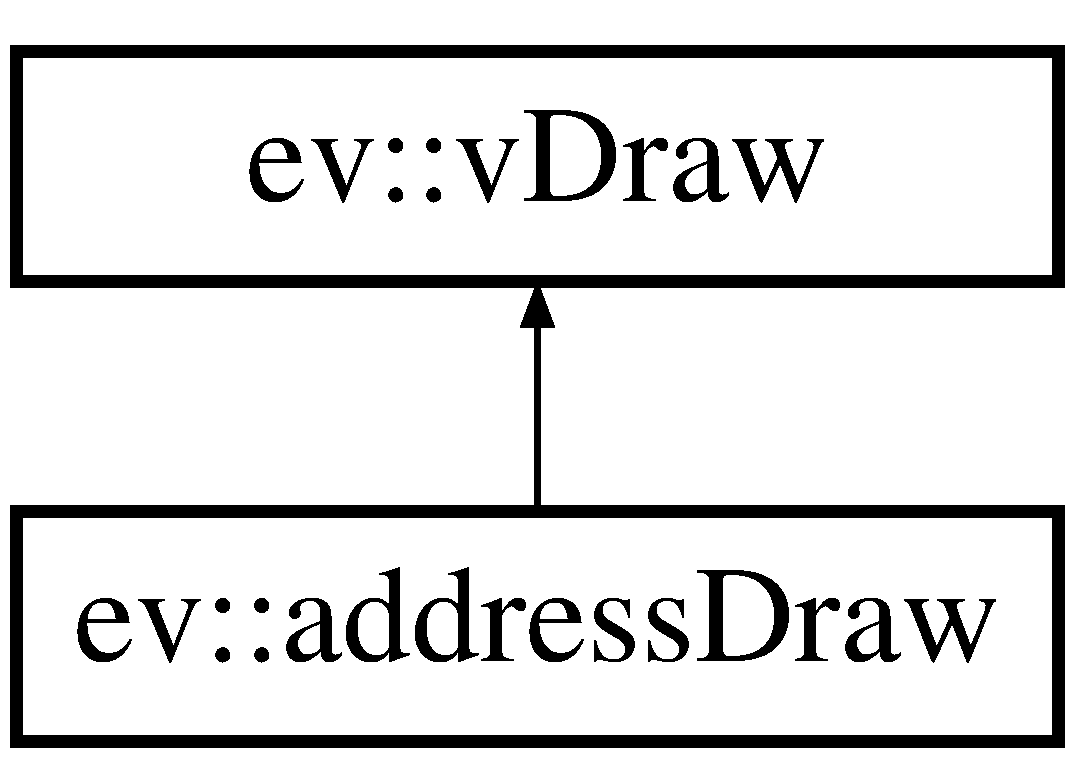
\includegraphics[height=2.000000cm]{classev_1_1addressDraw}
\end{center}
\end{figure}
\subsection*{Public Member Functions}
\begin{DoxyCompactItemize}
\item 
virtual void \hyperlink{classev_1_1addressDraw_a9ff5e558766f8b6cec2b11a60907b455}{draw} (cv\+::\+Mat \&image, const ev\+::v\+Queue \&e\+Set, int v\+Time)
\begin{DoxyCompactList}\small\item\em draw takes an image and overlays the new visualisation textures \end{DoxyCompactList}\item 
virtual std\+::string \hyperlink{classev_1_1addressDraw_a92e98d08d1fdbf47d7e0cb9fcf7a9937}{get\+Draw\+Type} ()
\begin{DoxyCompactList}\small\item\em get\+Tag returns the unique code for this drawing method. The arguments given on the command line must match this code exactly \end{DoxyCompactList}\item 
\mbox{\Hypertarget{classev_1_1addressDraw_a9bc65ede4756bf6a6bcbd10a085eb0cb}\label{classev_1_1addressDraw_a9bc65ede4756bf6a6bcbd10a085eb0cb}} 
virtual std\+::string {\bfseries get\+Event\+Type} ()
\end{DoxyCompactItemize}
\subsection*{Static Public Attributes}
\begin{DoxyCompactItemize}
\item 
\mbox{\Hypertarget{classev_1_1addressDraw_a224f9727090703d652a8e1ac793ca96e}\label{classev_1_1addressDraw_a224f9727090703d652a8e1ac793ca96e}} 
static const std\+::string {\bfseries drawtype} = \char`\"{}AE\char`\"{}
\end{DoxyCompactItemize}
\subsection*{Additional Inherited Members}


\subsection{Member Function Documentation}
\mbox{\Hypertarget{classev_1_1addressDraw_a9ff5e558766f8b6cec2b11a60907b455}\label{classev_1_1addressDraw_a9ff5e558766f8b6cec2b11a60907b455}} 
\index{ev\+::address\+Draw@{ev\+::address\+Draw}!draw@{draw}}
\index{draw@{draw}!ev\+::address\+Draw@{ev\+::address\+Draw}}
\subsubsection{\texorpdfstring{draw()}{draw()}}
{\footnotesize\ttfamily void ev\+::address\+Draw\+::draw (\begin{DoxyParamCaption}\item[{cv\+::\+Mat \&}]{canvas,  }\item[{const ev\+::v\+Queue \&}]{e\+Set,  }\item[{int}]{v\+Time }\end{DoxyParamCaption})\hspace{0.3cm}{\ttfamily [virtual]}}



draw takes an image and overlays the new visualisation textures 


\begin{DoxyParams}{Parameters}
{\em canvas} & is the image which may or may not yet exist \\
\hline
{\em e\+Set} & is the set of events which could possibly be drawn \\
\hline
\end{DoxyParams}


Implements \hyperlink{classev_1_1vDraw_af1eee5dcdf3b4cfee6a3024e5cd706f8}{ev\+::v\+Draw}.

\mbox{\Hypertarget{classev_1_1addressDraw_a92e98d08d1fdbf47d7e0cb9fcf7a9937}\label{classev_1_1addressDraw_a92e98d08d1fdbf47d7e0cb9fcf7a9937}} 
\index{ev\+::address\+Draw@{ev\+::address\+Draw}!get\+Draw\+Type@{get\+Draw\+Type}}
\index{get\+Draw\+Type@{get\+Draw\+Type}!ev\+::address\+Draw@{ev\+::address\+Draw}}
\subsubsection{\texorpdfstring{get\+Draw\+Type()}{getDrawType()}}
{\footnotesize\ttfamily std\+::string ev\+::address\+Draw\+::get\+Draw\+Type (\begin{DoxyParamCaption}{ }\end{DoxyParamCaption})\hspace{0.3cm}{\ttfamily [virtual]}}



get\+Tag returns the unique code for this drawing method. The arguments given on the command line must match this code exactly 

\begin{DoxyReturn}{Returns}
the tag code 
\end{DoxyReturn}


Implements \hyperlink{classev_1_1vDraw_ac01381befeffef2b930cbceb28b18a28}{ev\+::v\+Draw}.



The documentation for this class was generated from the following files\+:\begin{DoxyCompactItemize}
\item 
/mnt/d/projects/event-\/driven/lib/include/event-\/driven/v\+Draw.\+h\item 
/mnt/d/projects/event-\/driven/lib/src/v\+Draw\+\_\+basic.\+cpp\end{DoxyCompactItemize}

\hypertarget{classev_1_1AddressEvent}{}\section{ev\+:\+:Address\+Event Class Reference}
\label{classev_1_1AddressEvent}\index{ev\+::\+Address\+Event@{ev\+::\+Address\+Event}}


an event with a pixel location, camera number and polarity  




{\ttfamily \#include $<$v\+Codec.\+h$>$}

Inheritance diagram for ev\+:\+:Address\+Event\+:\begin{figure}[H]
\begin{center}
\leavevmode
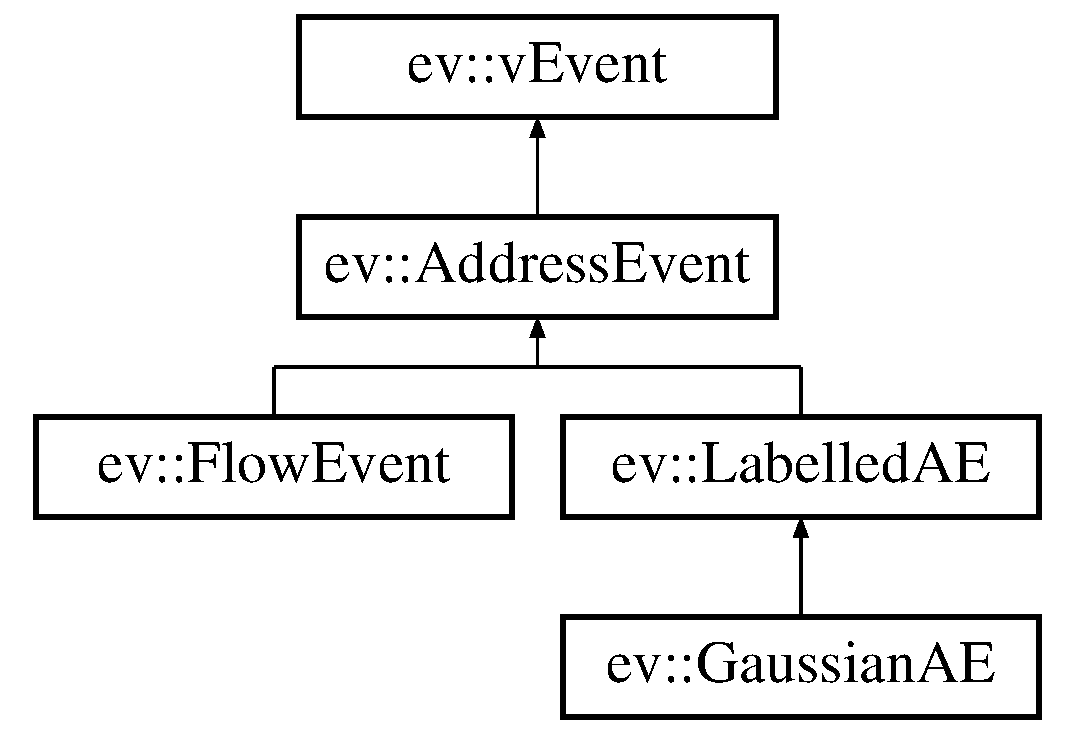
\includegraphics[height=4.000000cm]{classev_1_1AddressEvent}
\end{center}
\end{figure}
\subsection*{Public Member Functions}
\begin{DoxyCompactItemize}
\item 
\mbox{\Hypertarget{classev_1_1AddressEvent_a62e810ce50e155828957e61c99a165d2}\label{classev_1_1AddressEvent_a62e810ce50e155828957e61c99a165d2}} 
{\bfseries Address\+Event} (const \hyperlink{classev_1_1vEvent}{v\+Event} \&v)
\item 
\mbox{\Hypertarget{classev_1_1AddressEvent_a5072b43ca93fdcdf0294ecff78f3b424}\label{classev_1_1AddressEvent_a5072b43ca93fdcdf0294ecff78f3b424}} 
{\bfseries Address\+Event} (const \hyperlink{classev_1_1AddressEvent}{Address\+Event} \&v)
\item 
\mbox{\Hypertarget{classev_1_1AddressEvent_adabe75246de88f722d65b4994c7955eb}\label{classev_1_1AddressEvent_adabe75246de88f722d65b4994c7955eb}} 
virtual event {\bfseries clone} ()
\item 
\mbox{\Hypertarget{classev_1_1AddressEvent_a88fd7ed5398113959b148b3ff48dc9bb}\label{classev_1_1AddressEvent_a88fd7ed5398113959b148b3ff48dc9bb}} 
virtual void {\bfseries encode} (yarp\+::os\+::\+Bottle \&b) const
\item 
\mbox{\Hypertarget{classev_1_1AddressEvent_ab61870d54423584f9c1c5e48bf989df9}\label{classev_1_1AddressEvent_ab61870d54423584f9c1c5e48bf989df9}} 
virtual void {\bfseries encode} (std\+::vector$<$ int32\+\_\+t $>$ \&b, unsigned int \&pos) const
\item 
\mbox{\Hypertarget{classev_1_1AddressEvent_aadf6cc5f4681b4c4028ac2be4317ed55}\label{classev_1_1AddressEvent_aadf6cc5f4681b4c4028ac2be4317ed55}} 
virtual bool {\bfseries decode} (const yarp\+::os\+::\+Bottle \&packet, size\+\_\+t \&pos)
\item 
\mbox{\Hypertarget{classev_1_1AddressEvent_a0f898c7319ceb94bf6c5eb688ef1df46}\label{classev_1_1AddressEvent_a0f898c7319ceb94bf6c5eb688ef1df46}} 
virtual void {\bfseries decode} (const int32\+\_\+t $\ast$\&data)
\item 
\mbox{\Hypertarget{classev_1_1AddressEvent_a8defcdc4c7ab81cae0c608ef3d5c1dec}\label{classev_1_1AddressEvent_a8defcdc4c7ab81cae0c608ef3d5c1dec}} 
virtual yarp\+::os\+::\+Property {\bfseries get\+Content} () const
\item 
\mbox{\Hypertarget{classev_1_1AddressEvent_ab052f9d6d9ba89660e2e1c1e3dff07e9}\label{classev_1_1AddressEvent_ab052f9d6d9ba89660e2e1c1e3dff07e9}} 
virtual std\+::string {\bfseries get\+Type} () const
\item 
\mbox{\Hypertarget{classev_1_1AddressEvent_a4f0e15a8300d1018cbb813fa83aedb43}\label{classev_1_1AddressEvent_a4f0e15a8300d1018cbb813fa83aedb43}} 
virtual int {\bfseries get\+Channel} () const
\item 
\mbox{\Hypertarget{classev_1_1AddressEvent_a50e188b1c5702cab67a2175b81c32767}\label{classev_1_1AddressEvent_a50e188b1c5702cab67a2175b81c32767}} 
virtual void {\bfseries set\+Channel} (const int channel)
\end{DoxyCompactItemize}
\subsection*{Public Attributes}
\begin{DoxyCompactItemize}
\item 
\mbox{\Hypertarget{classev_1_1AddressEvent_a359b9c530269e582a058112a34a48383}\label{classev_1_1AddressEvent_a359b9c530269e582a058112a34a48383}} 
\begin{tabbing}
xx\=xx\=xx\=xx\=xx\=xx\=xx\=xx\=xx\=\kill
union \{\\
\>uint32\_t {\bfseries \_coded\_data}\\
\mbox{\Hypertarget{unionev_1_1AddressEvent_1_1_0D1_a51f7d79230871a81eca60e6fe852b2df}\label{unionev_1_1AddressEvent_1_1_0D1_a51f7d79230871a81eca60e6fe852b2df}} 
\>struct \{\\
\>\>unsigned int {\bfseries polarity}:1\\
\>\>unsigned int {\bfseries x}:9\\
\>\>unsigned int {\bfseries \_xfill}:2\\
\>\>unsigned int {\bfseries y}:8\\
\>\>unsigned int {\bfseries \_yfill}:2\\
\>\>unsigned int {\bfseries channel}:1\\
\>\>unsigned int {\bfseries type}:1\\
\>\>unsigned int {\bfseries skin}:1\\
\>\>unsigned int {\bfseries \_fill}:7\\
\>\} \\
\}; \\

\end{tabbing}\end{DoxyCompactItemize}
\subsection*{Static Public Attributes}
\begin{DoxyCompactItemize}
\item 
\mbox{\Hypertarget{classev_1_1AddressEvent_a9a2d3e863964a1247ae4203a4ad2c646}\label{classev_1_1AddressEvent_a9a2d3e863964a1247ae4203a4ad2c646}} 
static const std\+::string {\bfseries tag} = \char`\"{}AE\char`\"{}
\end{DoxyCompactItemize}


\subsection{Detailed Description}
an event with a pixel location, camera number and polarity 

The documentation for this class was generated from the following files\+:\begin{DoxyCompactItemize}
\item 
/mnt/d/projects/event-\/driven/lib/include/event-\/driven/v\+Codec.\+h\item 
/mnt/d/projects/event-\/driven/lib/src/codecs/codec\+\_\+\+Address\+Event.\+cpp\end{DoxyCompactItemize}

\hypertarget{classev_1_1benchmark}{}\section{ev\+:\+:benchmark Class Reference}
\label{classev_1_1benchmark}\index{ev\+::benchmark@{ev\+::benchmark}}
\subsection*{Public Member Functions}
\begin{DoxyCompactItemize}
\item 
\mbox{\Hypertarget{classev_1_1benchmark_a10722bcfcf5df8e34fc2f17e0247290f}\label{classev_1_1benchmark_a10722bcfcf5df8e34fc2f17e0247290f}} 
bool {\bfseries is\+Ready} ()
\item 
\mbox{\Hypertarget{classev_1_1benchmark_a23509b8f8895bafdb36e8bccfc14f82b}\label{classev_1_1benchmark_a23509b8f8895bafdb36e8bccfc14f82b}} 
double {\bfseries get\+Processor\+Usage} ()
\end{DoxyCompactItemize}


The documentation for this class was generated from the following files\+:\begin{DoxyCompactItemize}
\item 
/mnt/d/projects/event-\/driven/lib/include/event-\/driven/vts\+Helper.\+h\item 
/mnt/d/projects/event-\/driven/lib/src/vts\+Helper.\+cpp\end{DoxyCompactItemize}

\hypertarget{classev_1_1clusterDraw}{}\section{ev\+:\+:cluster\+Draw Class Reference}
\label{classev_1_1clusterDraw}\index{ev\+::cluster\+Draw@{ev\+::cluster\+Draw}}
Inheritance diagram for ev\+:\+:cluster\+Draw\+:\begin{figure}[H]
\begin{center}
\leavevmode
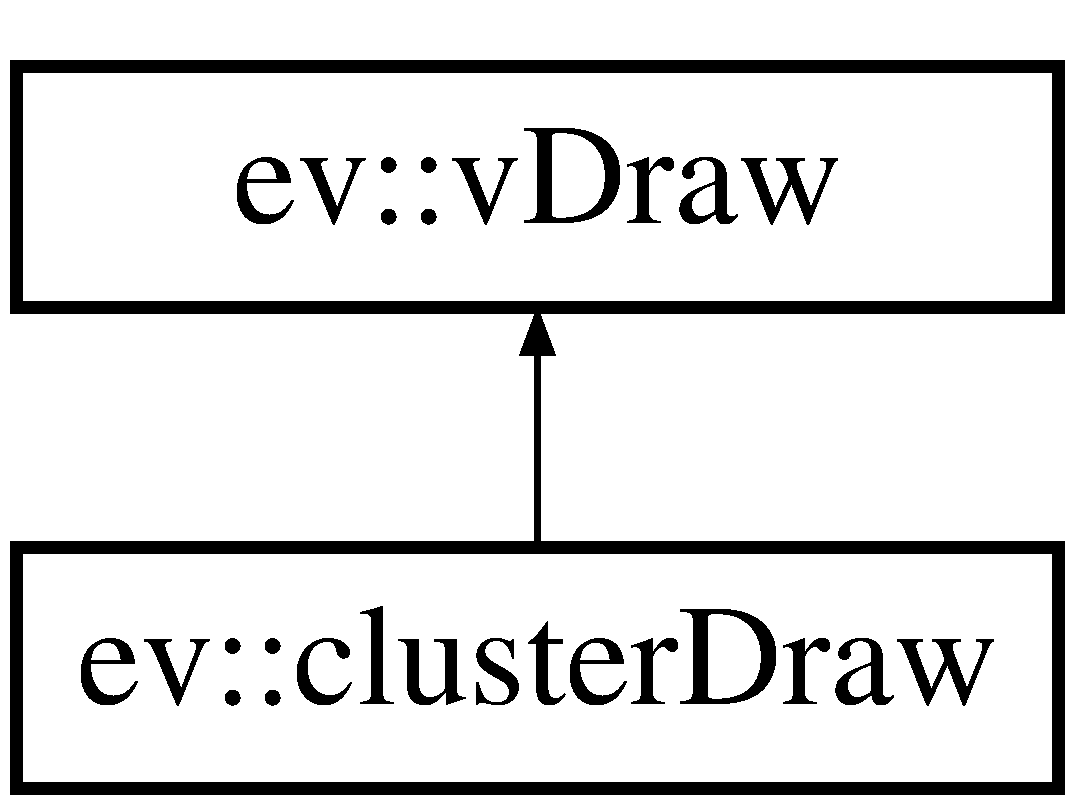
\includegraphics[height=2.000000cm]{classev_1_1clusterDraw}
\end{center}
\end{figure}
\subsection*{Public Member Functions}
\begin{DoxyCompactItemize}
\item 
virtual void \hyperlink{classev_1_1clusterDraw_aa70978bb98c7bde912eb03288f21cbb5}{draw} (cv\+::\+Mat \&image, const ev\+::v\+Queue \&e\+Set, int v\+Time)
\begin{DoxyCompactList}\small\item\em draw takes an image and overlays the new visualisation textures \end{DoxyCompactList}\item 
virtual std\+::string \hyperlink{classev_1_1clusterDraw_a21cd4ba2277ad5258b39d135e445b32f}{get\+Draw\+Type} ()
\begin{DoxyCompactList}\small\item\em get\+Tag returns the unique code for this drawing method. The arguments given on the command line must match this code exactly \end{DoxyCompactList}\item 
\mbox{\Hypertarget{classev_1_1clusterDraw_acfac944ed03a27cb408629fa2e9e44b7}\label{classev_1_1clusterDraw_acfac944ed03a27cb408629fa2e9e44b7}} 
virtual std\+::string {\bfseries get\+Event\+Type} ()
\end{DoxyCompactItemize}
\subsection*{Static Public Attributes}
\begin{DoxyCompactItemize}
\item 
\mbox{\Hypertarget{classev_1_1clusterDraw_ad498fb53993170b82b0116a43a3afd57}\label{classev_1_1clusterDraw_ad498fb53993170b82b0116a43a3afd57}} 
static const std\+::string {\bfseries drawtype} = \char`\"{}C\+LE\char`\"{}
\end{DoxyCompactItemize}
\subsection*{Protected Attributes}
\begin{DoxyCompactItemize}
\item 
\mbox{\Hypertarget{classev_1_1clusterDraw_ae6c0e0349720c63461e9a9124cef8e5e}\label{classev_1_1clusterDraw_ae6c0e0349720c63461e9a9124cef8e5e}} 
std\+::map$<$ int, ev\+::event$<$ \hyperlink{classev_1_1GaussianAE}{ev\+::\+Gaussian\+AE} $>$ $>$ {\bfseries persistance}
\item 
\mbox{\Hypertarget{classev_1_1clusterDraw_a7e4aa3579dc604914af2a5b21e35a0e6}\label{classev_1_1clusterDraw_a7e4aa3579dc604914af2a5b21e35a0e6}} 
int {\bfseries stagnant\+Count}
\end{DoxyCompactItemize}


\subsection{Member Function Documentation}
\mbox{\Hypertarget{classev_1_1clusterDraw_aa70978bb98c7bde912eb03288f21cbb5}\label{classev_1_1clusterDraw_aa70978bb98c7bde912eb03288f21cbb5}} 
\index{ev\+::cluster\+Draw@{ev\+::cluster\+Draw}!draw@{draw}}
\index{draw@{draw}!ev\+::cluster\+Draw@{ev\+::cluster\+Draw}}
\subsubsection{\texorpdfstring{draw()}{draw()}}
{\footnotesize\ttfamily void ev\+::cluster\+Draw\+::draw (\begin{DoxyParamCaption}\item[{cv\+::\+Mat \&}]{canvas,  }\item[{const ev\+::v\+Queue \&}]{e\+Set,  }\item[{int}]{v\+Time }\end{DoxyParamCaption})\hspace{0.3cm}{\ttfamily [virtual]}}



draw takes an image and overlays the new visualisation textures 


\begin{DoxyParams}{Parameters}
{\em canvas} & is the image which may or may not yet exist \\
\hline
{\em e\+Set} & is the set of events which could possibly be drawn \\
\hline
\end{DoxyParams}


Implements \hyperlink{classev_1_1vDraw_af1eee5dcdf3b4cfee6a3024e5cd706f8}{ev\+::v\+Draw}.

\mbox{\Hypertarget{classev_1_1clusterDraw_a21cd4ba2277ad5258b39d135e445b32f}\label{classev_1_1clusterDraw_a21cd4ba2277ad5258b39d135e445b32f}} 
\index{ev\+::cluster\+Draw@{ev\+::cluster\+Draw}!get\+Draw\+Type@{get\+Draw\+Type}}
\index{get\+Draw\+Type@{get\+Draw\+Type}!ev\+::cluster\+Draw@{ev\+::cluster\+Draw}}
\subsubsection{\texorpdfstring{get\+Draw\+Type()}{getDrawType()}}
{\footnotesize\ttfamily std\+::string ev\+::cluster\+Draw\+::get\+Draw\+Type (\begin{DoxyParamCaption}{ }\end{DoxyParamCaption})\hspace{0.3cm}{\ttfamily [virtual]}}



get\+Tag returns the unique code for this drawing method. The arguments given on the command line must match this code exactly 

\begin{DoxyReturn}{Returns}
the tag code 
\end{DoxyReturn}


Implements \hyperlink{classev_1_1vDraw_ac01381befeffef2b930cbceb28b18a28}{ev\+::v\+Draw}.



The documentation for this class was generated from the following files\+:\begin{DoxyCompactItemize}
\item 
/mnt/d/projects/event-\/driven/lib/include/event-\/driven/v\+Draw.\+h\item 
/mnt/d/projects/event-\/driven/lib/src/v\+Draw\+\_\+basic.\+cpp\end{DoxyCompactItemize}

\hypertarget{classev_1_1cochleaDraw}{}\section{ev\+:\+:cochlea\+Draw Class Reference}
\label{classev_1_1cochleaDraw}\index{ev\+::cochlea\+Draw@{ev\+::cochlea\+Draw}}
Inheritance diagram for ev\+:\+:cochlea\+Draw\+:\begin{figure}[H]
\begin{center}
\leavevmode
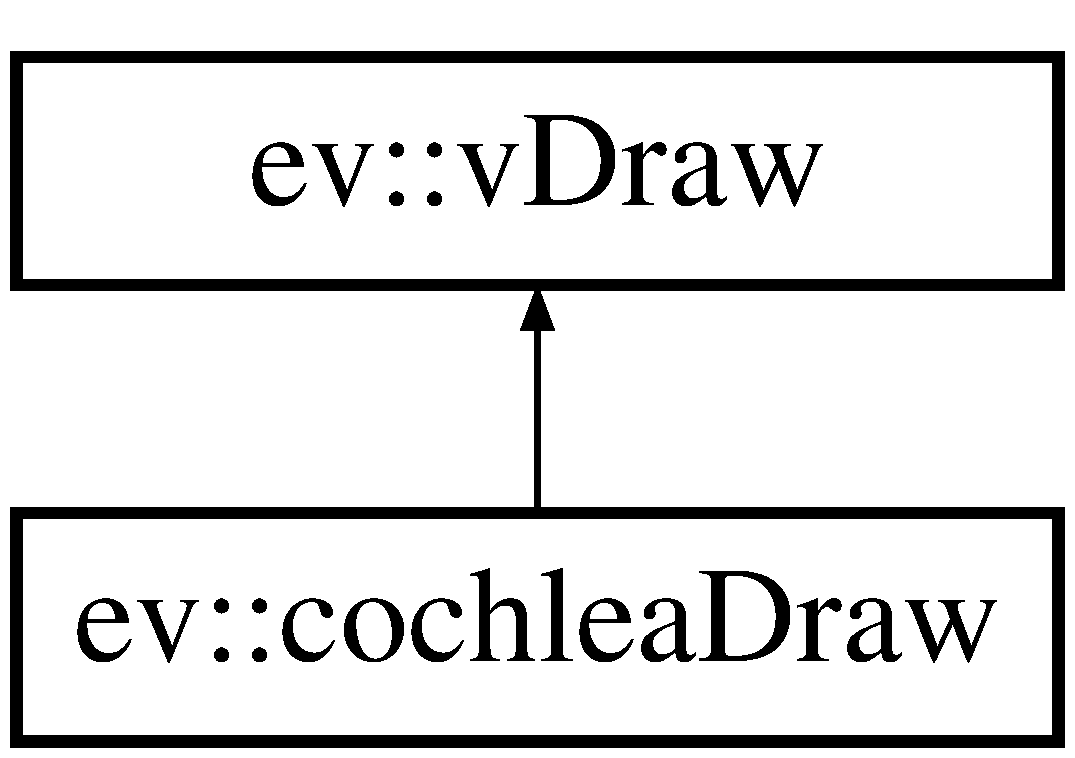
\includegraphics[height=2.000000cm]{classev_1_1cochleaDraw}
\end{center}
\end{figure}
\subsection*{Public Member Functions}
\begin{DoxyCompactItemize}
\item 
virtual void \hyperlink{classev_1_1cochleaDraw_a2b06c53991065506fcdaa9afec8282af}{draw} (cv\+::\+Mat \&image, const ev\+::v\+Queue \&e\+Set, int v\+Time)
\begin{DoxyCompactList}\small\item\em draw takes an image and overlays the new visualisation textures \end{DoxyCompactList}\item 
virtual std\+::string \hyperlink{classev_1_1cochleaDraw_a722aac2b6c1af1f6691721beb8a25325}{get\+Draw\+Type} ()
\begin{DoxyCompactList}\small\item\em get\+Tag returns the unique code for this drawing method. The arguments given on the command line must match this code exactly \end{DoxyCompactList}\item 
\mbox{\Hypertarget{classev_1_1cochleaDraw_afa164b9b693c4b0c41737c9ae35b2cef}\label{classev_1_1cochleaDraw_afa164b9b693c4b0c41737c9ae35b2cef}} 
virtual std\+::string {\bfseries get\+Event\+Type} ()
\end{DoxyCompactItemize}
\subsection*{Static Public Attributes}
\begin{DoxyCompactItemize}
\item 
\mbox{\Hypertarget{classev_1_1cochleaDraw_a649ade5bf1b9b8ba53b365d3103c76b9}\label{classev_1_1cochleaDraw_a649ade5bf1b9b8ba53b365d3103c76b9}} 
static const std\+::string {\bfseries drawtype} = \char`\"{}E\+AR\char`\"{}
\end{DoxyCompactItemize}
\subsection*{Additional Inherited Members}


\subsection{Member Function Documentation}
\mbox{\Hypertarget{classev_1_1cochleaDraw_a2b06c53991065506fcdaa9afec8282af}\label{classev_1_1cochleaDraw_a2b06c53991065506fcdaa9afec8282af}} 
\index{ev\+::cochlea\+Draw@{ev\+::cochlea\+Draw}!draw@{draw}}
\index{draw@{draw}!ev\+::cochlea\+Draw@{ev\+::cochlea\+Draw}}
\subsubsection{\texorpdfstring{draw()}{draw()}}
{\footnotesize\ttfamily void ev\+::cochlea\+Draw\+::draw (\begin{DoxyParamCaption}\item[{cv\+::\+Mat \&}]{canvas,  }\item[{const ev\+::v\+Queue \&}]{e\+Set,  }\item[{int}]{v\+Time }\end{DoxyParamCaption})\hspace{0.3cm}{\ttfamily [virtual]}}



draw takes an image and overlays the new visualisation textures 


\begin{DoxyParams}{Parameters}
{\em canvas} & is the image which may or may not yet exist \\
\hline
{\em e\+Set} & is the set of events which could possibly be drawn \\
\hline
\end{DoxyParams}


Implements \hyperlink{classev_1_1vDraw_af1eee5dcdf3b4cfee6a3024e5cd706f8}{ev\+::v\+Draw}.

\mbox{\Hypertarget{classev_1_1cochleaDraw_a722aac2b6c1af1f6691721beb8a25325}\label{classev_1_1cochleaDraw_a722aac2b6c1af1f6691721beb8a25325}} 
\index{ev\+::cochlea\+Draw@{ev\+::cochlea\+Draw}!get\+Draw\+Type@{get\+Draw\+Type}}
\index{get\+Draw\+Type@{get\+Draw\+Type}!ev\+::cochlea\+Draw@{ev\+::cochlea\+Draw}}
\subsubsection{\texorpdfstring{get\+Draw\+Type()}{getDrawType()}}
{\footnotesize\ttfamily std\+::string ev\+::cochlea\+Draw\+::get\+Draw\+Type (\begin{DoxyParamCaption}{ }\end{DoxyParamCaption})\hspace{0.3cm}{\ttfamily [virtual]}}



get\+Tag returns the unique code for this drawing method. The arguments given on the command line must match this code exactly 

\begin{DoxyReturn}{Returns}
the tag code 
\end{DoxyReturn}


Implements \hyperlink{classev_1_1vDraw_ac01381befeffef2b930cbceb28b18a28}{ev\+::v\+Draw}.



The documentation for this class was generated from the following files\+:\begin{DoxyCompactItemize}
\item 
/mnt/d/projects/event-\/driven/lib/include/event-\/driven/v\+Draw.\+h\item 
/mnt/d/projects/event-\/driven/lib/src/v\+Draw\+\_\+basic.\+cpp\end{DoxyCompactItemize}

\hypertarget{classev_1_1collectorPort}{}\section{ev\+:\+:collector\+Port Class Reference}
\label{classev_1_1collectorPort}\index{ev\+::collector\+Port@{ev\+::collector\+Port}}


an output port that can safely accept events from multiple threads and sends them at a fixed output rate.  




{\ttfamily \#include $<$v\+Collect\+Send.\+h$>$}

Inheritance diagram for ev\+:\+:collector\+Port\+:\begin{figure}[H]
\begin{center}
\leavevmode
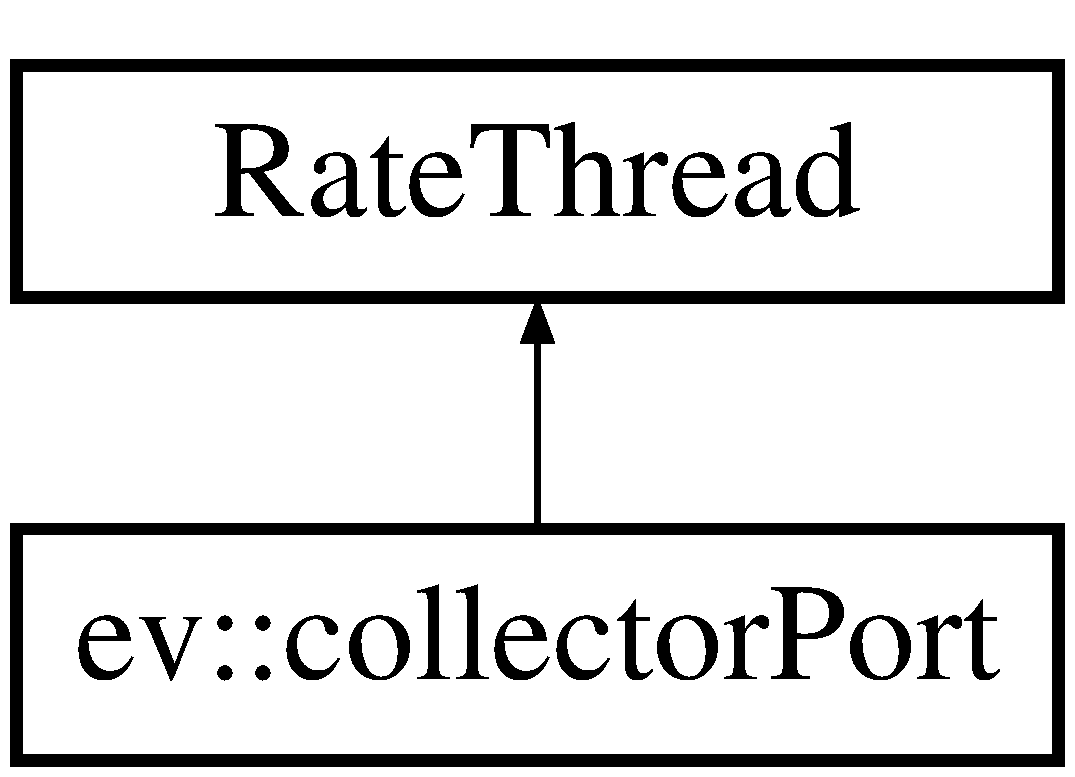
\includegraphics[height=2.000000cm]{classev_1_1collectorPort}
\end{center}
\end{figure}
\subsection*{Public Member Functions}
\begin{DoxyCompactItemize}
\item 
\mbox{\Hypertarget{classev_1_1collectorPort_ac7cd1de9c40bd46df66b67ae824bb258}\label{classev_1_1collectorPort_ac7cd1de9c40bd46df66b67ae824bb258}} 
\hyperlink{classev_1_1collectorPort_ac7cd1de9c40bd46df66b67ae824bb258}{collector\+Port} ()
\begin{DoxyCompactList}\small\item\em constructor \end{DoxyCompactList}\item 
\mbox{\Hypertarget{classev_1_1collectorPort_a164072ae38c4e115873c451984b8e7f4}\label{classev_1_1collectorPort_a164072ae38c4e115873c451984b8e7f4}} 
bool \hyperlink{classev_1_1collectorPort_a164072ae38c4e115873c451984b8e7f4}{open} (std\+::string name)
\begin{DoxyCompactList}\small\item\em open the output port \end{DoxyCompactList}\item 
\mbox{\Hypertarget{classev_1_1collectorPort_ab1d587f6b728b65b22df73bbe674607d}\label{classev_1_1collectorPort_ab1d587f6b728b65b22df73bbe674607d}} 
void \hyperlink{classev_1_1collectorPort_ab1d587f6b728b65b22df73bbe674607d}{pushevent} (event$<$$>$ v, yarp\+::os\+::\+Stamp y)
\begin{DoxyCompactList}\small\item\em add an event to be sent on next thread execution \end{DoxyCompactList}\item 
\mbox{\Hypertarget{classev_1_1collectorPort_a7ec227ae78ec71ca8867a20ae815ea7d}\label{classev_1_1collectorPort_a7ec227ae78ec71ca8867a20ae815ea7d}} 
void \hyperlink{classev_1_1collectorPort_a7ec227ae78ec71ca8867a20ae815ea7d}{run} ()
\begin{DoxyCompactList}\small\item\em on each call of the thread, all events that have been added are sent on the port in a \hyperlink{classev_1_1vBottle}{v\+Bottle}. If no events have been added, a \hyperlink{classev_1_1vBottle}{v\+Bottle} is not sent. \end{DoxyCompactList}\end{DoxyCompactItemize}


\subsection{Detailed Description}
an output port that can safely accept events from multiple threads and sends them at a fixed output rate. 

The documentation for this class was generated from the following file\+:\begin{DoxyCompactItemize}
\item 
/mnt/d/projects/event-\/driven/lib/include/event-\/driven/v\+Collect\+Send.\+h\end{DoxyCompactItemize}

\hypertarget{classexampleModule}{}\section{example\+Module Class Reference}
\label{classexampleModule}\index{example\+Module@{example\+Module}}
Inheritance diagram for example\+Module\+:\begin{figure}[H]
\begin{center}
\leavevmode
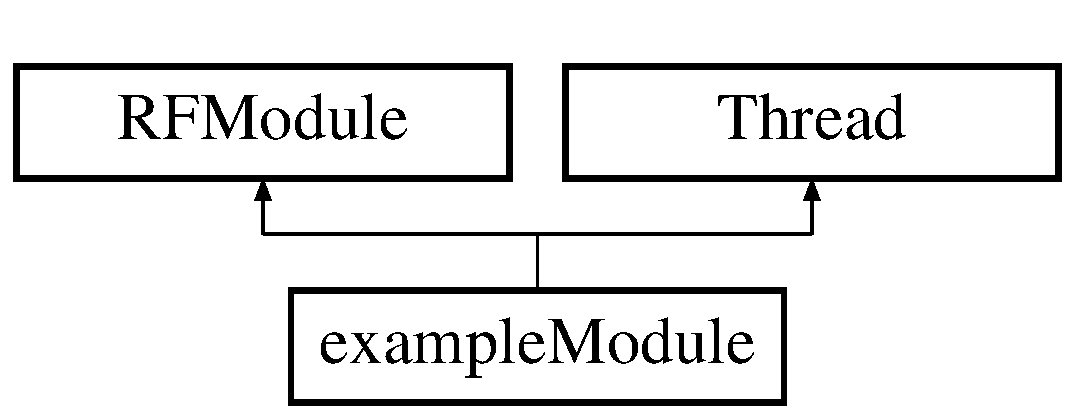
\includegraphics[height=2.000000cm]{classexampleModule}
\end{center}
\end{figure}
\subsection*{Public Member Functions}
\begin{DoxyCompactItemize}
\item 
\mbox{\Hypertarget{classexampleModule_ad4d614a75a36e54b416b95ce48e23809}\label{classexampleModule_ad4d614a75a36e54b416b95ce48e23809}} 
virtual bool {\bfseries configure} (yarp\+::os\+::\+Resource\+Finder \&rf)
\item 
\mbox{\Hypertarget{classexampleModule_a9316bf049434e746a26242f30226f0ff}\label{classexampleModule_a9316bf049434e746a26242f30226f0ff}} 
virtual double {\bfseries get\+Period} ()
\item 
\mbox{\Hypertarget{classexampleModule_af7f744b259d435200d1669d138d6c6cd}\label{classexampleModule_af7f744b259d435200d1669d138d6c6cd}} 
bool {\bfseries interrupt\+Module} ()
\item 
\mbox{\Hypertarget{classexampleModule_a5263e596f82ccaf25f39e41c399c23aa}\label{classexampleModule_a5263e596f82ccaf25f39e41c399c23aa}} 
void {\bfseries on\+Stop} ()
\item 
\mbox{\Hypertarget{classexampleModule_ae2b99b0679b122d2aeb53aa44f106f55}\label{classexampleModule_ae2b99b0679b122d2aeb53aa44f106f55}} 
virtual bool {\bfseries update\+Module} ()
\item 
\mbox{\Hypertarget{classexampleModule_a62c8579890452322481beb0f6aedb1a4}\label{classexampleModule_a62c8579890452322481beb0f6aedb1a4}} 
void {\bfseries run} ()
\end{DoxyCompactItemize}


The documentation for this class was generated from the following file\+:\begin{DoxyCompactItemize}
\item 
/mnt/d/projects/event-\/driven/documentation/example-\/module/example-\/module.\+cpp\end{DoxyCompactItemize}

\hypertarget{classev_1_1fixedSurface}{}\section{ev\+:\+:fixed\+Surface Class Reference}
\label{classev_1_1fixedSurface}\index{ev\+::fixed\+Surface@{ev\+::fixed\+Surface}}


a spatio-\/temporal surface storing only a fixed number of events  




{\ttfamily \#include $<$v\+Window\+\_\+adv.\+h$>$}

Inheritance diagram for ev\+:\+:fixed\+Surface\+:\begin{figure}[H]
\begin{center}
\leavevmode
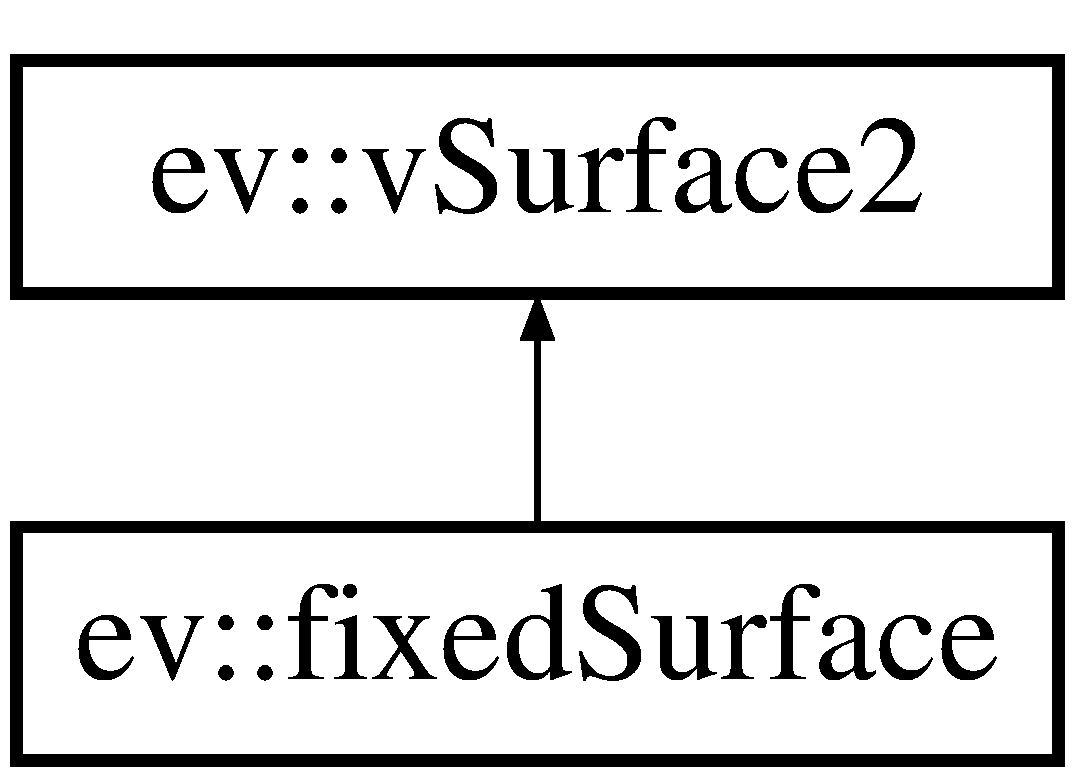
\includegraphics[height=2.000000cm]{classev_1_1fixedSurface}
\end{center}
\end{figure}
\subsection*{Public Member Functions}
\begin{DoxyCompactItemize}
\item 
\mbox{\Hypertarget{classev_1_1fixedSurface_adee898e7c65c9c8d41fd20530d9f10b0}\label{classev_1_1fixedSurface_adee898e7c65c9c8d41fd20530d9f10b0}} 
{\bfseries fixed\+Surface} (int qlength=2000, int \hyperlink{classev_1_1vSurface2_a1aa8027816352a15d5b9bf1f26f48e76}{width}=128, int height=128)
\item 
\mbox{\Hypertarget{classev_1_1fixedSurface_ace012acf57456f71d77fc7a349a915d7}\label{classev_1_1fixedSurface_ace012acf57456f71d77fc7a349a915d7}} 
virtual v\+Queue {\bfseries remove\+Events} (event$<$$>$ to\+Add)
\item 
\mbox{\Hypertarget{classev_1_1fixedSurface_a317c375340f308fda67c6da2074f0e0e}\label{classev_1_1fixedSurface_a317c375340f308fda67c6da2074f0e0e}} 
virtual void {\bfseries fast\+Remove\+Events} (event$<$$>$ to\+Add)
\item 
\mbox{\Hypertarget{classev_1_1fixedSurface_ac8249b63b5ada0491d6a6ff70b745488}\label{classev_1_1fixedSurface_ac8249b63b5ada0491d6a6ff70b745488}} 
void {\bfseries set\+Fixed\+Window\+Size} (int length)
\end{DoxyCompactItemize}
\subsection*{Additional Inherited Members}


\subsection{Detailed Description}
a spatio-\/temporal surface storing only a fixed number of events 

The documentation for this class was generated from the following files\+:\begin{DoxyCompactItemize}
\item 
/mnt/d/projects/event-\/driven/lib/include/event-\/driven/v\+Window\+\_\+adv.\+h\item 
/mnt/d/projects/event-\/driven/lib/src/v\+Window\+\_\+adv.\+cpp\end{DoxyCompactItemize}

\hypertarget{classev_1_1flowDraw}{}\section{ev\+:\+:flow\+Draw Class Reference}
\label{classev_1_1flowDraw}\index{ev\+::flow\+Draw@{ev\+::flow\+Draw}}
Inheritance diagram for ev\+:\+:flow\+Draw\+:\begin{figure}[H]
\begin{center}
\leavevmode
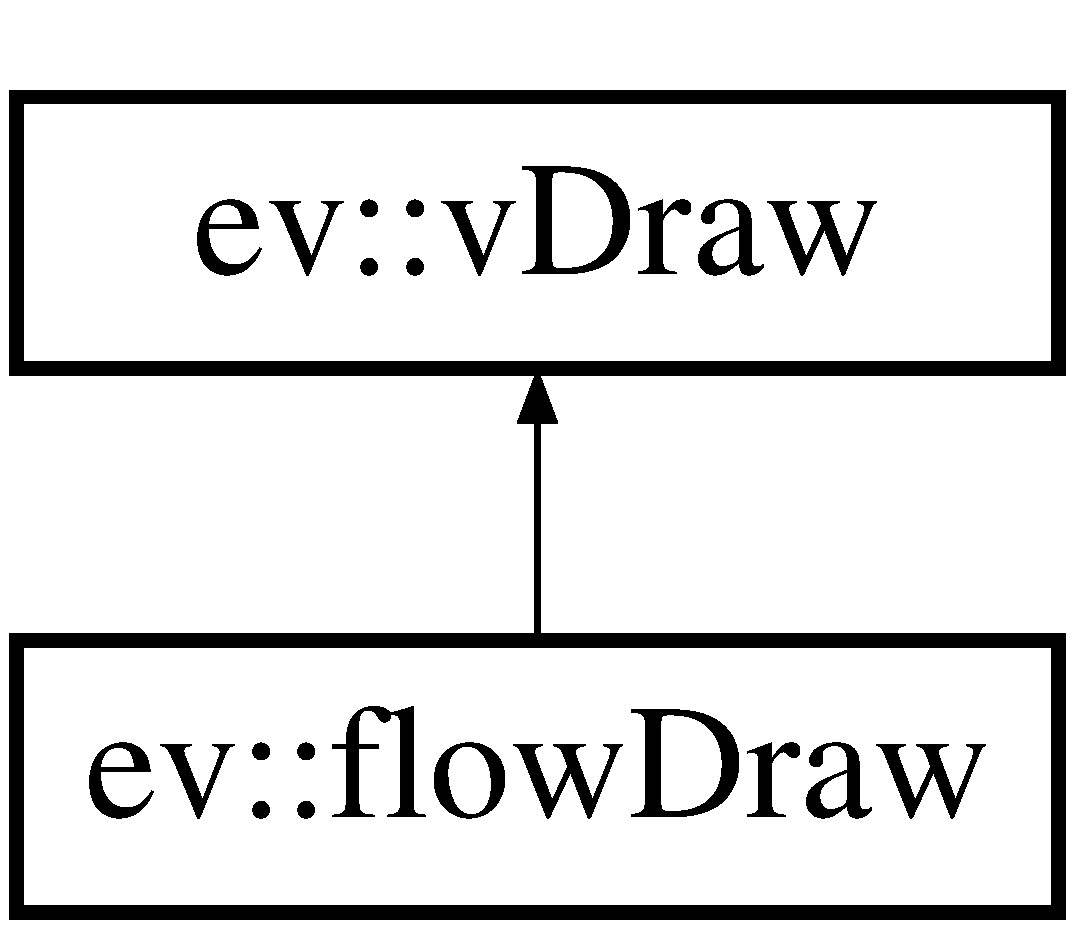
\includegraphics[height=2.000000cm]{classev_1_1flowDraw}
\end{center}
\end{figure}
\subsection*{Public Member Functions}
\begin{DoxyCompactItemize}
\item 
virtual void \hyperlink{classev_1_1flowDraw_a15d97ddaf93734a912be64fb60977ee2}{draw} (cv\+::\+Mat \&image, const ev\+::v\+Queue \&e\+Set, int v\+Time)
\begin{DoxyCompactList}\small\item\em draw takes an image and overlays the new visualisation textures \end{DoxyCompactList}\item 
virtual std\+::string \hyperlink{classev_1_1flowDraw_a6caf6d848d79407e62b7bf13c58d583e}{get\+Draw\+Type} ()
\begin{DoxyCompactList}\small\item\em get\+Tag returns the unique code for this drawing method. The arguments given on the command line must match this code exactly \end{DoxyCompactList}\item 
\mbox{\Hypertarget{classev_1_1flowDraw_ad70fa4b0401da0c426802fe185b3c1b8}\label{classev_1_1flowDraw_ad70fa4b0401da0c426802fe185b3c1b8}} 
virtual std\+::string {\bfseries get\+Event\+Type} ()
\end{DoxyCompactItemize}
\subsection*{Static Public Attributes}
\begin{DoxyCompactItemize}
\item 
\mbox{\Hypertarget{classev_1_1flowDraw_a6ff0f7b973f6dda5923e399b4abdcc3c}\label{classev_1_1flowDraw_a6ff0f7b973f6dda5923e399b4abdcc3c}} 
static const std\+::string {\bfseries drawtype} = \char`\"{}F\+L\+OW\char`\"{}
\end{DoxyCompactItemize}
\subsection*{Additional Inherited Members}


\subsection{Member Function Documentation}
\mbox{\Hypertarget{classev_1_1flowDraw_a15d97ddaf93734a912be64fb60977ee2}\label{classev_1_1flowDraw_a15d97ddaf93734a912be64fb60977ee2}} 
\index{ev\+::flow\+Draw@{ev\+::flow\+Draw}!draw@{draw}}
\index{draw@{draw}!ev\+::flow\+Draw@{ev\+::flow\+Draw}}
\subsubsection{\texorpdfstring{draw()}{draw()}}
{\footnotesize\ttfamily void ev\+::flow\+Draw\+::draw (\begin{DoxyParamCaption}\item[{cv\+::\+Mat \&}]{canvas,  }\item[{const ev\+::v\+Queue \&}]{e\+Set,  }\item[{int}]{v\+Time }\end{DoxyParamCaption})\hspace{0.3cm}{\ttfamily [virtual]}}



draw takes an image and overlays the new visualisation textures 


\begin{DoxyParams}{Parameters}
{\em canvas} & is the image which may or may not yet exist \\
\hline
{\em e\+Set} & is the set of events which could possibly be drawn \\
\hline
\end{DoxyParams}


Implements \hyperlink{classev_1_1vDraw_af1eee5dcdf3b4cfee6a3024e5cd706f8}{ev\+::v\+Draw}.

\mbox{\Hypertarget{classev_1_1flowDraw_a6caf6d848d79407e62b7bf13c58d583e}\label{classev_1_1flowDraw_a6caf6d848d79407e62b7bf13c58d583e}} 
\index{ev\+::flow\+Draw@{ev\+::flow\+Draw}!get\+Draw\+Type@{get\+Draw\+Type}}
\index{get\+Draw\+Type@{get\+Draw\+Type}!ev\+::flow\+Draw@{ev\+::flow\+Draw}}
\subsubsection{\texorpdfstring{get\+Draw\+Type()}{getDrawType()}}
{\footnotesize\ttfamily std\+::string ev\+::flow\+Draw\+::get\+Draw\+Type (\begin{DoxyParamCaption}{ }\end{DoxyParamCaption})\hspace{0.3cm}{\ttfamily [virtual]}}



get\+Tag returns the unique code for this drawing method. The arguments given on the command line must match this code exactly 

\begin{DoxyReturn}{Returns}
the tag code 
\end{DoxyReturn}


Implements \hyperlink{classev_1_1vDraw_ac01381befeffef2b930cbceb28b18a28}{ev\+::v\+Draw}.



The documentation for this class was generated from the following files\+:\begin{DoxyCompactItemize}
\item 
/mnt/d/projects/event-\/driven/lib/include/event-\/driven/v\+Draw.\+h\item 
/mnt/d/projects/event-\/driven/lib/src/v\+Draw\+\_\+basic.\+cpp\end{DoxyCompactItemize}

\hypertarget{classev_1_1FlowEvent}{}\section{ev\+:\+:Flow\+Event Class Reference}
\label{classev_1_1FlowEvent}\index{ev\+::\+Flow\+Event@{ev\+::\+Flow\+Event}}


an \hyperlink{classev_1_1AddressEvent}{Address\+Event} with a velocity in visual space  




{\ttfamily \#include $<$v\+Codec.\+h$>$}

Inheritance diagram for ev\+:\+:Flow\+Event\+:\begin{figure}[H]
\begin{center}
\leavevmode
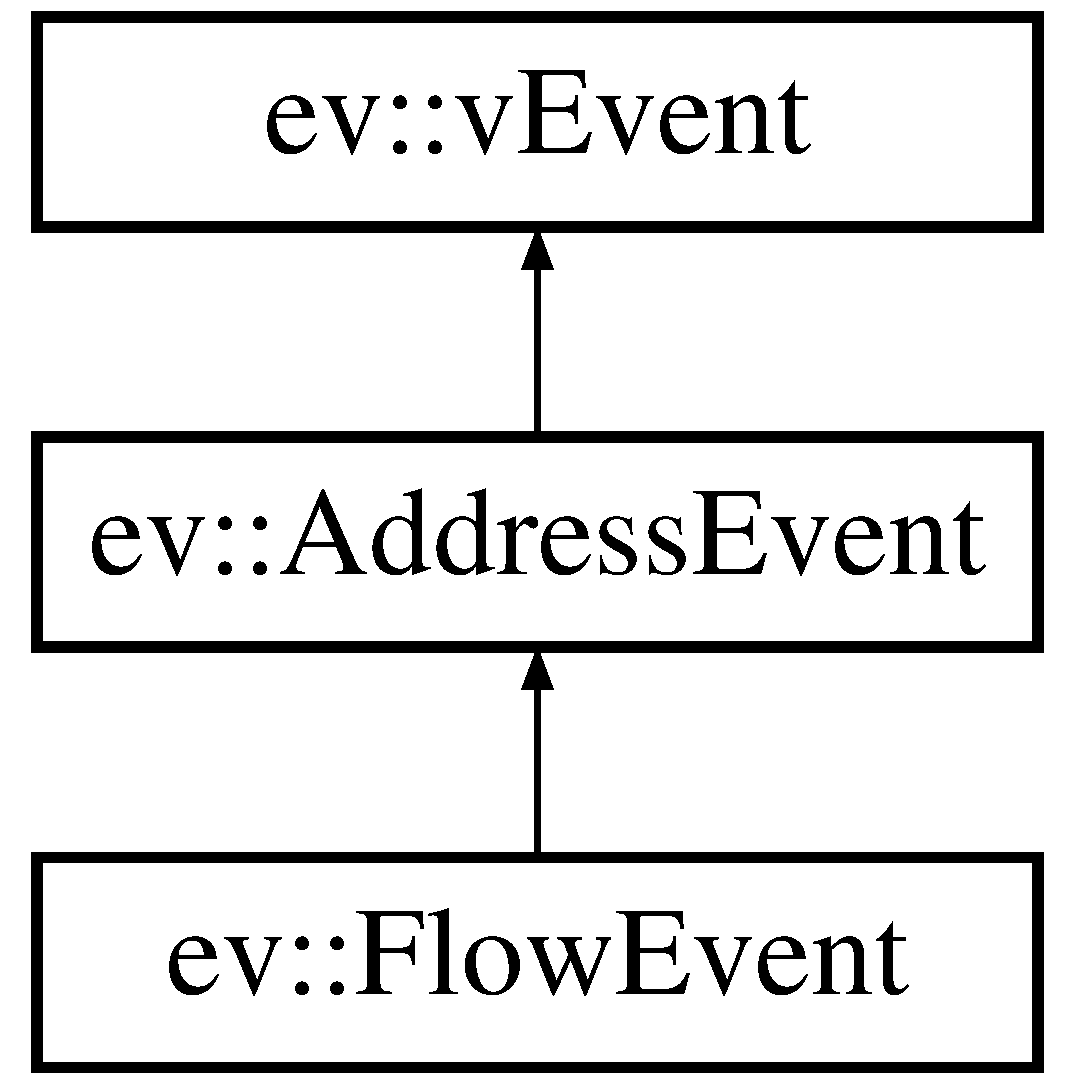
\includegraphics[height=3.000000cm]{classev_1_1FlowEvent}
\end{center}
\end{figure}
\subsection*{Public Member Functions}
\begin{DoxyCompactItemize}
\item 
\mbox{\Hypertarget{classev_1_1FlowEvent_aa268bbbeb75a7ec0634e7eff9bf9dda5}\label{classev_1_1FlowEvent_aa268bbbeb75a7ec0634e7eff9bf9dda5}} 
{\bfseries Flow\+Event} (const \hyperlink{classev_1_1vEvent}{v\+Event} \&v)
\item 
\mbox{\Hypertarget{classev_1_1FlowEvent_a0784e0ce0b0b1fb1d9c61f8134efa70b}\label{classev_1_1FlowEvent_a0784e0ce0b0b1fb1d9c61f8134efa70b}} 
{\bfseries Flow\+Event} (const \hyperlink{classev_1_1FlowEvent}{Flow\+Event} \&v)
\item 
\mbox{\Hypertarget{classev_1_1FlowEvent_a6a108ba6028ea69a9398745074d7300f}\label{classev_1_1FlowEvent_a6a108ba6028ea69a9398745074d7300f}} 
virtual event {\bfseries clone} ()
\item 
\mbox{\Hypertarget{classev_1_1FlowEvent_a5105689e47975ead26caf7b68b62463e}\label{classev_1_1FlowEvent_a5105689e47975ead26caf7b68b62463e}} 
virtual void {\bfseries encode} (yarp\+::os\+::\+Bottle \&b) const
\item 
\mbox{\Hypertarget{classev_1_1FlowEvent_a4861e688ba3175ab80f0e2cbd3cc477b}\label{classev_1_1FlowEvent_a4861e688ba3175ab80f0e2cbd3cc477b}} 
virtual void {\bfseries encode} (std\+::vector$<$ int32\+\_\+t $>$ \&b, unsigned int \&pos) const
\item 
\mbox{\Hypertarget{classev_1_1FlowEvent_a0c6e4d68d303d9cc4016959dc065c12a}\label{classev_1_1FlowEvent_a0c6e4d68d303d9cc4016959dc065c12a}} 
virtual bool {\bfseries decode} (const yarp\+::os\+::\+Bottle \&packet, size\+\_\+t \&pos)
\item 
\mbox{\Hypertarget{classev_1_1FlowEvent_af10d2b90b62f4c45dffc33abea193d09}\label{classev_1_1FlowEvent_af10d2b90b62f4c45dffc33abea193d09}} 
virtual void {\bfseries decode} (const int32\+\_\+t $\ast$\&data)
\item 
\mbox{\Hypertarget{classev_1_1FlowEvent_affda6cd024d5edc8d9d437d3194cc8c4}\label{classev_1_1FlowEvent_affda6cd024d5edc8d9d437d3194cc8c4}} 
virtual yarp\+::os\+::\+Property {\bfseries get\+Content} () const
\item 
\mbox{\Hypertarget{classev_1_1FlowEvent_ab2544edc7563366b97bf69c229b797fe}\label{classev_1_1FlowEvent_ab2544edc7563366b97bf69c229b797fe}} 
virtual std\+::string {\bfseries get\+Type} () const
\item 
\mbox{\Hypertarget{classev_1_1FlowEvent_a550ab5ead40a7107247a64ab83492002}\label{classev_1_1FlowEvent_a550ab5ead40a7107247a64ab83492002}} 
int {\bfseries get\+Death} () const
\end{DoxyCompactItemize}
\subsection*{Public Attributes}
\begin{DoxyCompactItemize}
\item 
\mbox{\Hypertarget{classev_1_1FlowEvent_a6f7cdf3ec22ead9e2faaebd4a213279f}\label{classev_1_1FlowEvent_a6f7cdf3ec22ead9e2faaebd4a213279f}} 
\begin{tabbing}
xx\=xx\=xx\=xx\=xx\=xx\=xx\=xx\=xx\=\kill
union \{\\
\>uint32\_t {\bfseries \_fei} \mbox{[}2\mbox{]}\\
\mbox{\Hypertarget{unionev_1_1FlowEvent_1_1_0D9_a174994f064562221bd6c96077d16eeb9}\label{unionev_1_1FlowEvent_1_1_0D9_a174994f064562221bd6c96077d16eeb9}} 
\>struct \{\\
\>\>float {\bfseries vx}\\
\>\>float {\bfseries vy}\\
\>\} \\
\}; \\

\end{tabbing}\end{DoxyCompactItemize}
\subsection*{Static Public Attributes}
\begin{DoxyCompactItemize}
\item 
\mbox{\Hypertarget{classev_1_1FlowEvent_a583ae9aaa6cbcbe1779eab526b5df1de}\label{classev_1_1FlowEvent_a583ae9aaa6cbcbe1779eab526b5df1de}} 
static const std\+::string {\bfseries tag} = \char`\"{}F\+L\+OW\char`\"{}
\end{DoxyCompactItemize}


\subsection{Detailed Description}
an \hyperlink{classev_1_1AddressEvent}{Address\+Event} with a velocity in visual space 

The documentation for this class was generated from the following files\+:\begin{DoxyCompactItemize}
\item 
/mnt/d/projects/event-\/driven/lib/include/event-\/driven/v\+Codec.\+h\item 
/mnt/d/projects/event-\/driven/lib/src/codecs/codec\+\_\+\+Flow\+Event.\+cpp\end{DoxyCompactItemize}

\hypertarget{classev_1_1GaussianAE}{}\section{ev\+:\+:Gaussian\+AE Class Reference}
\label{classev_1_1GaussianAE}\index{ev\+::\+Gaussian\+AE@{ev\+::\+Gaussian\+AE}}


a \hyperlink{classev_1_1LabelledAE}{Labelled\+AE} with parameters that define a 2D gaussian  




{\ttfamily \#include $<$v\+Codec.\+h$>$}

Inheritance diagram for ev\+:\+:Gaussian\+AE\+:\begin{figure}[H]
\begin{center}
\leavevmode
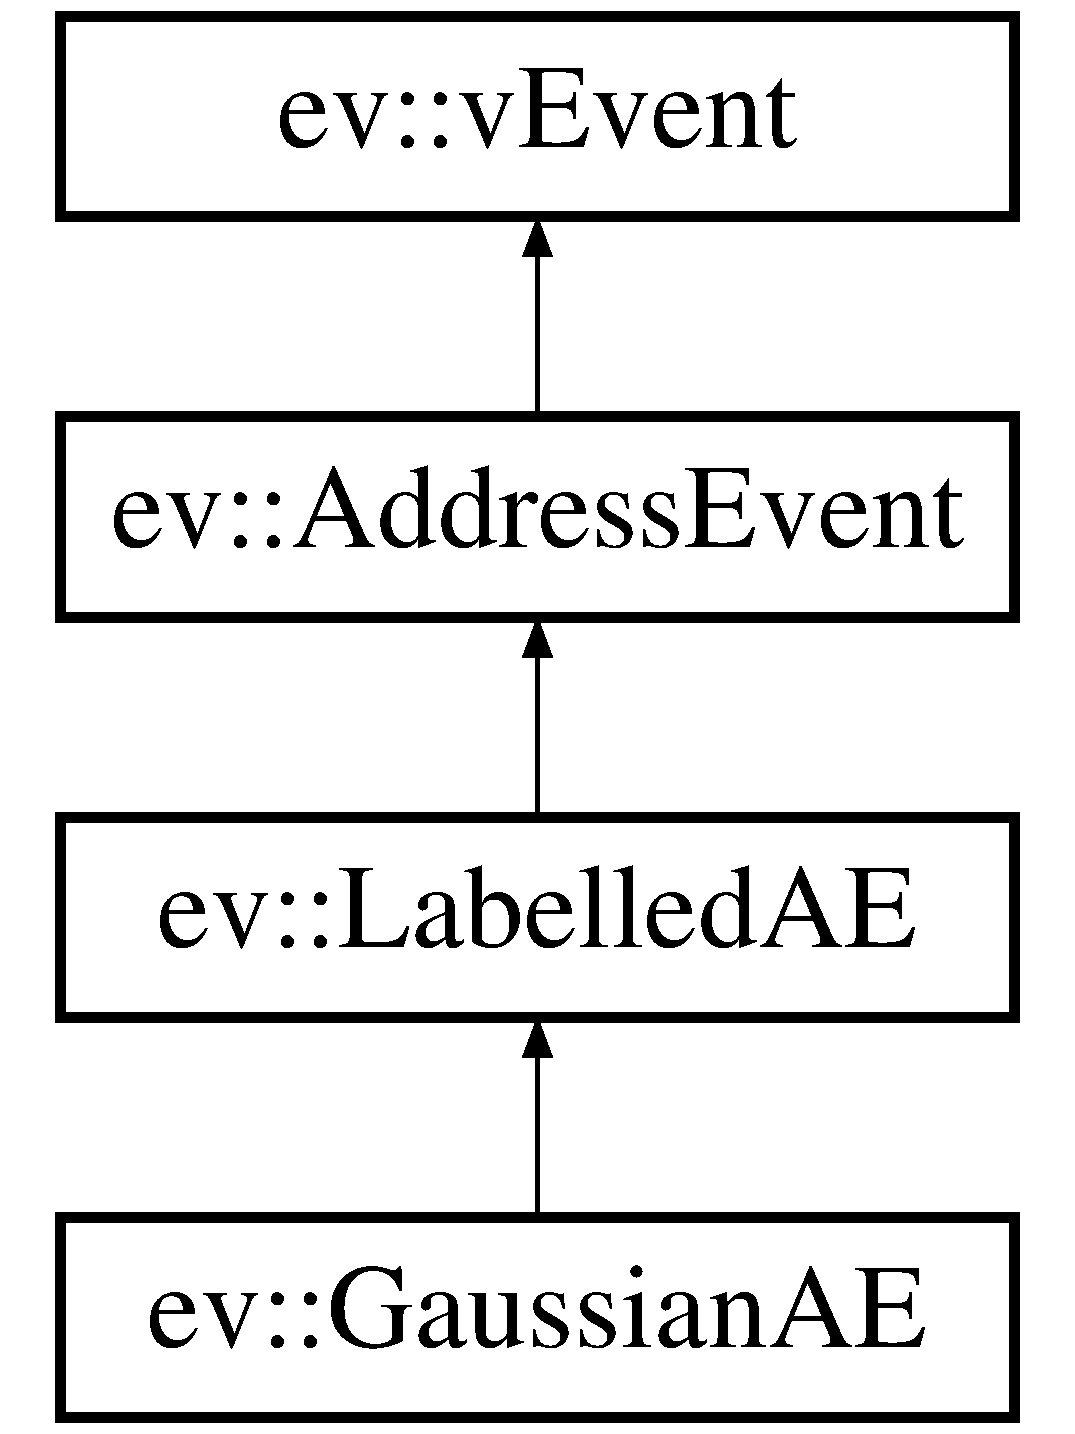
\includegraphics[height=4.000000cm]{classev_1_1GaussianAE}
\end{center}
\end{figure}
\subsection*{Public Member Functions}
\begin{DoxyCompactItemize}
\item 
\mbox{\Hypertarget{classev_1_1GaussianAE_abc9c34d68ad44ea743b565a6206e591f}\label{classev_1_1GaussianAE_abc9c34d68ad44ea743b565a6206e591f}} 
{\bfseries Gaussian\+AE} (const \hyperlink{classev_1_1vEvent}{v\+Event} \&v)
\item 
\mbox{\Hypertarget{classev_1_1GaussianAE_ac5934905f00cc08eb9c444f67e0ec6a2}\label{classev_1_1GaussianAE_ac5934905f00cc08eb9c444f67e0ec6a2}} 
{\bfseries Gaussian\+AE} (const \hyperlink{classev_1_1GaussianAE}{Gaussian\+AE} \&v)
\item 
\mbox{\Hypertarget{classev_1_1GaussianAE_aa9e649d9039d3e9348cea99352df77c5}\label{classev_1_1GaussianAE_aa9e649d9039d3e9348cea99352df77c5}} 
virtual event {\bfseries clone} ()
\item 
\mbox{\Hypertarget{classev_1_1GaussianAE_a8ac9f9d68e23134e64ab37215c4feadd}\label{classev_1_1GaussianAE_a8ac9f9d68e23134e64ab37215c4feadd}} 
virtual void {\bfseries encode} (yarp\+::os\+::\+Bottle \&b) const
\item 
\mbox{\Hypertarget{classev_1_1GaussianAE_a4f337114d2e9d3d142953525a6eb7418}\label{classev_1_1GaussianAE_a4f337114d2e9d3d142953525a6eb7418}} 
virtual void {\bfseries encode} (std\+::vector$<$ int32\+\_\+t $>$ \&b, unsigned int \&pos) const
\item 
\mbox{\Hypertarget{classev_1_1GaussianAE_a508515e443b7c3c5ffd1f3fd02ced00a}\label{classev_1_1GaussianAE_a508515e443b7c3c5ffd1f3fd02ced00a}} 
virtual bool {\bfseries decode} (const yarp\+::os\+::\+Bottle \&packet, size\+\_\+t \&pos)
\item 
\mbox{\Hypertarget{classev_1_1GaussianAE_aa24997795ded9df87a8013ca45bb4d20}\label{classev_1_1GaussianAE_aa24997795ded9df87a8013ca45bb4d20}} 
virtual void {\bfseries decode} (const int32\+\_\+t $\ast$\&data)
\item 
\mbox{\Hypertarget{classev_1_1GaussianAE_ad0738c9667722bbd4cc5cb786028dca6}\label{classev_1_1GaussianAE_ad0738c9667722bbd4cc5cb786028dca6}} 
virtual yarp\+::os\+::\+Property {\bfseries get\+Content} () const
\item 
\mbox{\Hypertarget{classev_1_1GaussianAE_acc5728386bc75bead01615c96ae4dab1}\label{classev_1_1GaussianAE_acc5728386bc75bead01615c96ae4dab1}} 
virtual std\+::string {\bfseries get\+Type} () const
\end{DoxyCompactItemize}
\subsection*{Public Attributes}
\begin{DoxyCompactItemize}
\item 
\mbox{\Hypertarget{classev_1_1GaussianAE_a13e0c15248195b159d6b672ea3596611}\label{classev_1_1GaussianAE_a13e0c15248195b159d6b672ea3596611}} 
\begin{tabbing}
xx\=xx\=xx\=xx\=xx\=xx\=xx\=xx\=xx\=\kill
union \{\\
\>uint32\_t {\bfseries \_gaei} \mbox{[}3\mbox{]}\\
\mbox{\Hypertarget{unionev_1_1GaussianAE_1_1_0D13_aebead89f411b9301f4fdb56ef30ba0c0}\label{unionev_1_1GaussianAE_1_1_0D13_aebead89f411b9301f4fdb56ef30ba0c0}} 
\>struct \{\\
\>\>float {\bfseries sigx}\\
\>\>float {\bfseries sigy}\\
\>\>float {\bfseries sigxy}\\
\>\} \\
\}; \\

\end{tabbing}\end{DoxyCompactItemize}
\subsection*{Static Public Attributes}
\begin{DoxyCompactItemize}
\item 
\mbox{\Hypertarget{classev_1_1GaussianAE_a6d0ea5de274ddd380b056d2ba8b019e2}\label{classev_1_1GaussianAE_a6d0ea5de274ddd380b056d2ba8b019e2}} 
static const std\+::string {\bfseries tag} = \char`\"{}G\+AE\char`\"{}
\end{DoxyCompactItemize}


\subsection{Detailed Description}
a \hyperlink{classev_1_1LabelledAE}{Labelled\+AE} with parameters that define a 2D gaussian 

The documentation for this class was generated from the following files\+:\begin{DoxyCompactItemize}
\item 
/mnt/d/projects/event-\/driven/lib/include/event-\/driven/v\+Codec.\+h\item 
/mnt/d/projects/event-\/driven/lib/src/codecs/codec\+\_\+\+Gaussian\+A\+E.\+cpp\end{DoxyCompactItemize}

\hypertarget{classev_1_1historicalSurface}{}\section{ev\+:\+:historical\+Surface Class Reference}
\label{classev_1_1historicalSurface}\index{ev\+::historical\+Surface@{ev\+::historical\+Surface}}


a surface that can be queried at any time in the past.  




{\ttfamily \#include $<$v\+Window\+\_\+adv.\+h$>$}

Inheritance diagram for ev\+:\+:historical\+Surface\+:\begin{figure}[H]
\begin{center}
\leavevmode
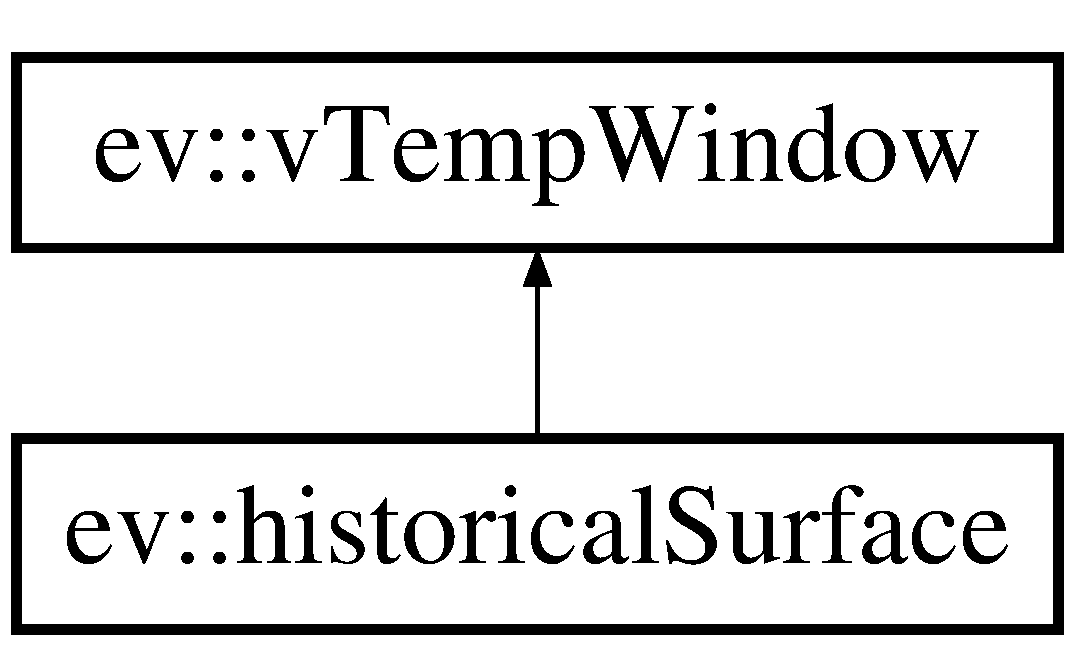
\includegraphics[height=2.000000cm]{classev_1_1historicalSurface}
\end{center}
\end{figure}
\subsection*{Public Member Functions}
\begin{DoxyCompactItemize}
\item 
\mbox{\Hypertarget{classev_1_1historicalSurface_adbe662bedcf6ee9c87f9b78d15c8ae85}\label{classev_1_1historicalSurface_adbe662bedcf6ee9c87f9b78d15c8ae85}} 
void {\bfseries initialise} (int height, int width)
\item 
\mbox{\Hypertarget{classev_1_1historicalSurface_a03476e5a9cff0d369fef76711c6ebea5}\label{classev_1_1historicalSurface_a03476e5a9cff0d369fef76711c6ebea5}} 
v\+Queue {\bfseries get\+Surface} (int query\+Time, int query\+Window)
\item 
\mbox{\Hypertarget{classev_1_1historicalSurface_a289a2d3cb116fb1cdb99d38b03d74dd0}\label{classev_1_1historicalSurface_a289a2d3cb116fb1cdb99d38b03d74dd0}} 
v\+Queue {\bfseries get\+Surface} (int query\+Time, int query\+Window, int d)
\item 
\mbox{\Hypertarget{classev_1_1historicalSurface_a10f0938bac2fc0b7a0f5624dfcd65f2f}\label{classev_1_1historicalSurface_a10f0938bac2fc0b7a0f5624dfcd65f2f}} 
v\+Queue {\bfseries get\+Surface} (int query\+Time, int query\+Window, int d, int x, int y)
\item 
\mbox{\Hypertarget{classev_1_1historicalSurface_a18830cb21753a190270bf03108c95f71}\label{classev_1_1historicalSurface_a18830cb21753a190270bf03108c95f71}} 
v\+Queue {\bfseries get\+Surface} (int query\+Time, int query\+Window, int xl, int xh, int yl, int yh)
\item 
\mbox{\Hypertarget{classev_1_1historicalSurface_ae423da2b112194abd11e837e7142a71d}\label{classev_1_1historicalSurface_ae423da2b112194abd11e837e7142a71d}} 
void {\bfseries get\+SurfaceN} (ev\+::v\+Queue \&qret, int query\+Time, int num\+Events, int d)
\item 
\mbox{\Hypertarget{classev_1_1historicalSurface_afa98f88d820fd48698a2470857440a81}\label{classev_1_1historicalSurface_afa98f88d820fd48698a2470857440a81}} 
void {\bfseries get\+SurfaceN} (ev\+::v\+Queue \&qret, int query\+Time, int num\+Events, int d, int x, int y)
\item 
\mbox{\Hypertarget{classev_1_1historicalSurface_a7d2fa665ed41226f22b90c11b3c2f00d}\label{classev_1_1historicalSurface_a7d2fa665ed41226f22b90c11b3c2f00d}} 
void {\bfseries get\+SurfaceN} (ev\+::v\+Queue \&qret, int query\+Time, int num\+Events, int xl, int xh, int yl, int yh)
\end{DoxyCompactItemize}
\subsection*{Additional Inherited Members}


\subsection{Detailed Description}
a surface that can be queried at any time in the past. 

The documentation for this class was generated from the following files\+:\begin{DoxyCompactItemize}
\item 
/mnt/d/projects/event-\/driven/lib/include/event-\/driven/v\+Window\+\_\+adv.\+h\item 
/mnt/d/projects/event-\/driven/lib/src/v\+Window\+\_\+adv.\+cpp\end{DoxyCompactItemize}

\hypertarget{classev_1_1hSurfThread}{}\section{ev\+:\+:h\+Surf\+Thread Class Reference}
\label{classev_1_1hSurfThread}\index{ev\+::h\+Surf\+Thread@{ev\+::h\+Surf\+Thread}}


asynchronously read events and push them in a \hyperlink{classev_1_1historicalSurface}{historical\+Surface}  




{\ttfamily \#include $<$v\+Surface\+Handler\+Th.\+h$>$}

Inheritance diagram for ev\+:\+:h\+Surf\+Thread\+:\begin{figure}[H]
\begin{center}
\leavevmode
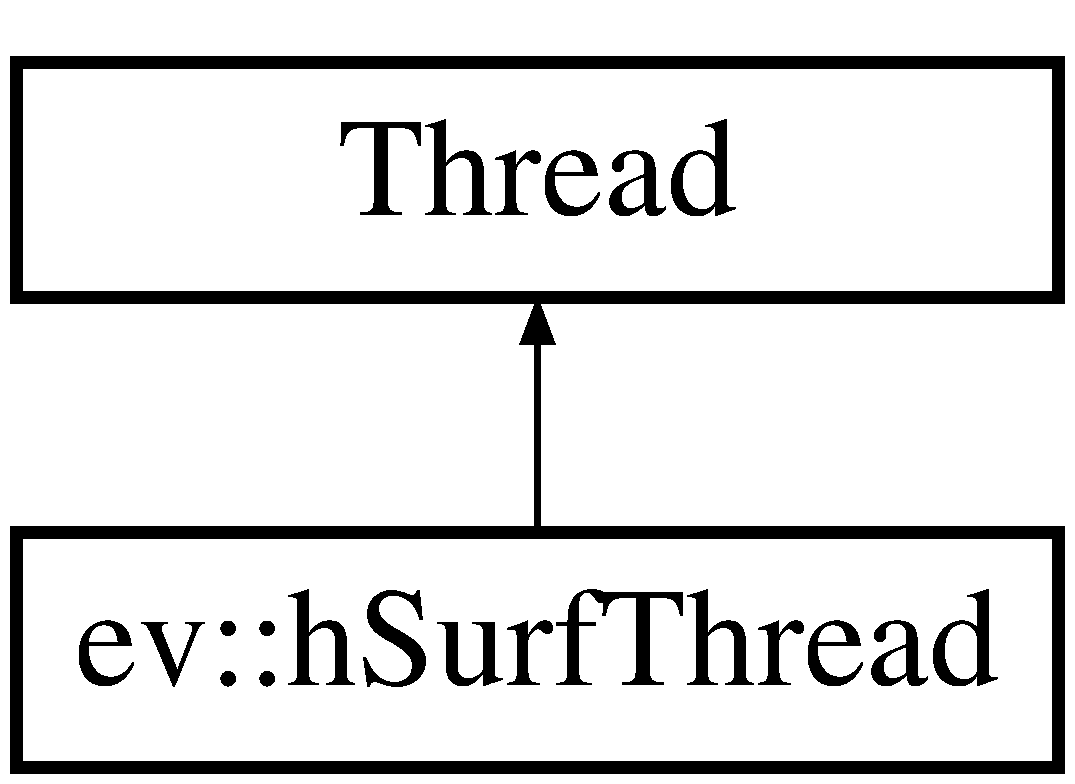
\includegraphics[height=2.000000cm]{classev_1_1hSurfThread}
\end{center}
\end{figure}
\subsection*{Public Member Functions}
\begin{DoxyCompactItemize}
\item 
\mbox{\Hypertarget{classev_1_1hSurfThread_a17acb3eb05f063ab81ab5128986ed7c8}\label{classev_1_1hSurfThread_a17acb3eb05f063ab81ab5128986ed7c8}} 
void {\bfseries configure} (int height, int width, double maxcpudelay)
\item 
\mbox{\Hypertarget{classev_1_1hSurfThread_afa2fc93ae2c64231e566738ebfddabf1}\label{classev_1_1hSurfThread_afa2fc93ae2c64231e566738ebfddabf1}} 
bool {\bfseries open} (std\+::string portname)
\item 
\mbox{\Hypertarget{classev_1_1hSurfThread_a7897b02f77738563c0d2fd5123dc4c51}\label{classev_1_1hSurfThread_a7897b02f77738563c0d2fd5123dc4c51}} 
void {\bfseries on\+Stop} ()
\item 
\mbox{\Hypertarget{classev_1_1hSurfThread_af4a0a8b35321419785dce1b94e43e5e3}\label{classev_1_1hSurfThread_af4a0a8b35321419785dce1b94e43e5e3}} 
void {\bfseries run} ()
\item 
\mbox{\Hypertarget{classev_1_1hSurfThread_a469e52e39fe123a6699171e504cf0e78}\label{classev_1_1hSurfThread_a469e52e39fe123a6699171e504cf0e78}} 
v\+Queue {\bfseries query\+R\+OI} (int channel, int num\+Evts, int r)
\item 
\mbox{\Hypertarget{classev_1_1hSurfThread_ada4a11e319f5f0122897e21d6411bb1a}\label{classev_1_1hSurfThread_ada4a11e319f5f0122897e21d6411bb1a}} 
v\+Queue {\bfseries query\+R\+OI} (int channel, unsigned int query\+Size, int x, int y, int r)
\item 
\mbox{\Hypertarget{classev_1_1hSurfThread_a89e485321978fdf785ba0e4e3b08a7ec}\label{classev_1_1hSurfThread_a89e485321978fdf785ba0e4e3b08a7ec}} 
v\+Queue {\bfseries query\+Window} (int channel, unsigned int query\+Size)
\item 
\mbox{\Hypertarget{classev_1_1hSurfThread_ae50c10e866f8692aae342d75e38369e7}\label{classev_1_1hSurfThread_ae50c10e866f8692aae342d75e38369e7}} 
double {\bfseries query\+Delay} (int channel=0)
\item 
\mbox{\Hypertarget{classev_1_1hSurfThread_a02f2a70c6f8147e70e1689520555c389}\label{classev_1_1hSurfThread_a02f2a70c6f8147e70e1689520555c389}} 
yarp\+::os\+::\+Stamp {\bfseries query\+Ystamp} ()
\item 
\mbox{\Hypertarget{classev_1_1hSurfThread_af5da61e8087f133f2202c873660779bc}\label{classev_1_1hSurfThread_af5da61e8087f133f2202c873660779bc}} 
int {\bfseries query\+Vstamp} (int channel=0)
\item 
\mbox{\Hypertarget{classev_1_1hSurfThread_a92089f336c6298e58440cee7f3b2eb07}\label{classev_1_1hSurfThread_a92089f336c6298e58440cee7f3b2eb07}} 
int {\bfseries query\+Q\+Delay} ()
\end{DoxyCompactItemize}


\subsection{Detailed Description}
asynchronously read events and push them in a \hyperlink{classev_1_1historicalSurface}{historical\+Surface} 

The documentation for this class was generated from the following file\+:\begin{DoxyCompactItemize}
\item 
/mnt/d/projects/event-\/driven/lib/include/event-\/driven/v\+Surface\+Handler\+Th.\+h\end{DoxyCompactItemize}

\hypertarget{classev_1_1imuDraw}{}\section{ev\+:\+:imu\+Draw Class Reference}
\label{classev_1_1imuDraw}\index{ev\+::imu\+Draw@{ev\+::imu\+Draw}}
Inheritance diagram for ev\+:\+:imu\+Draw\+:\begin{figure}[H]
\begin{center}
\leavevmode
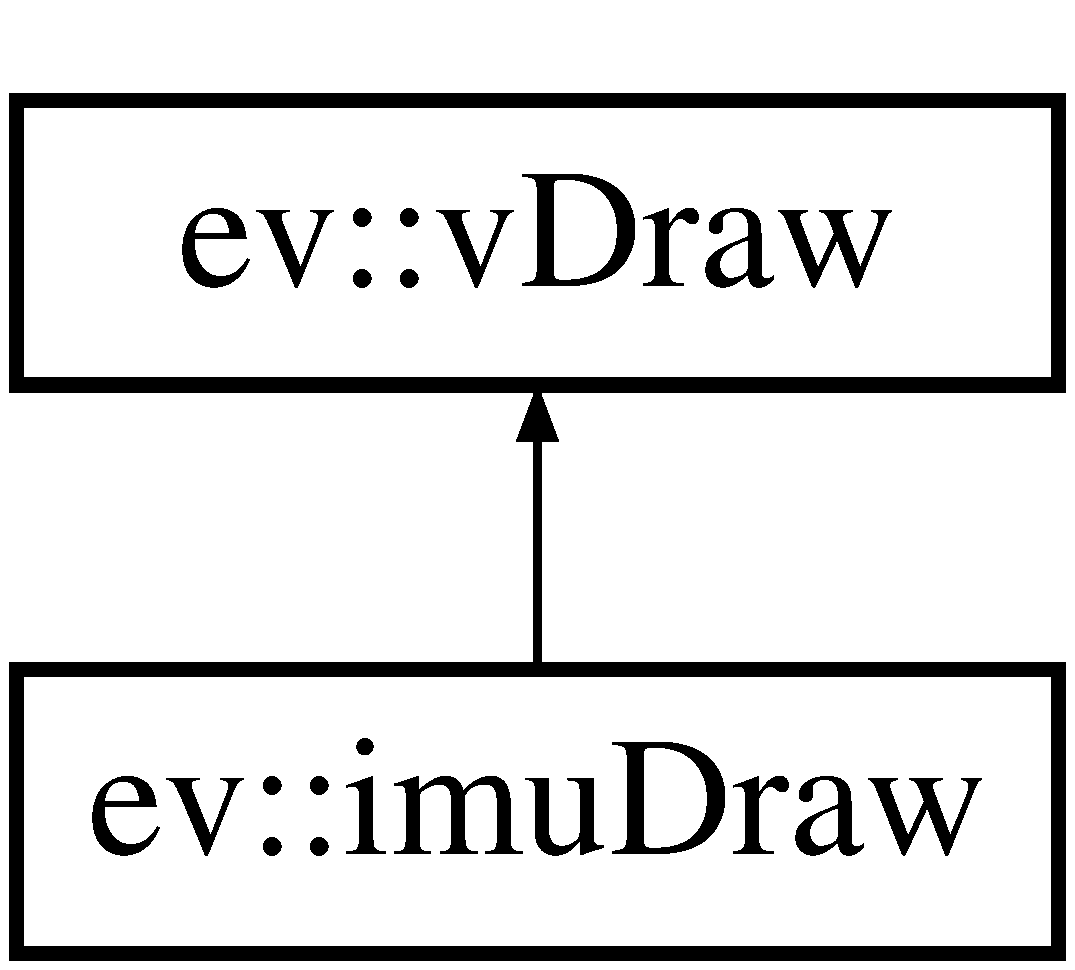
\includegraphics[height=2.000000cm]{classev_1_1imuDraw}
\end{center}
\end{figure}
\subsection*{Public Member Functions}
\begin{DoxyCompactItemize}
\item 
virtual void \hyperlink{classev_1_1imuDraw_addbaf0eff95fe6e791ca53c36218267e}{draw} (cv\+::\+Mat \&image, const ev\+::v\+Queue \&e\+Set, int v\+Time)
\begin{DoxyCompactList}\small\item\em draw takes an image and overlays the new visualisation textures \end{DoxyCompactList}\item 
virtual std\+::string \hyperlink{classev_1_1imuDraw_ab622b53cbe53421958cb7572919a0318}{get\+Draw\+Type} ()
\begin{DoxyCompactList}\small\item\em get\+Tag returns the unique code for this drawing method. The arguments given on the command line must match this code exactly \end{DoxyCompactList}\item 
\mbox{\Hypertarget{classev_1_1imuDraw_a21d47d10bbafe24e9633ec464d6fd060}\label{classev_1_1imuDraw_a21d47d10bbafe24e9633ec464d6fd060}} 
virtual std\+::string {\bfseries get\+Event\+Type} ()
\end{DoxyCompactItemize}
\subsection*{Static Public Attributes}
\begin{DoxyCompactItemize}
\item 
\mbox{\Hypertarget{classev_1_1imuDraw_a2447e11bc738f17ed6d46da1ad542ca0}\label{classev_1_1imuDraw_a2447e11bc738f17ed6d46da1ad542ca0}} 
static const std\+::string {\bfseries drawtype} = \char`\"{}I\+MU\char`\"{}
\end{DoxyCompactItemize}
\subsection*{Additional Inherited Members}


\subsection{Member Function Documentation}
\mbox{\Hypertarget{classev_1_1imuDraw_addbaf0eff95fe6e791ca53c36218267e}\label{classev_1_1imuDraw_addbaf0eff95fe6e791ca53c36218267e}} 
\index{ev\+::imu\+Draw@{ev\+::imu\+Draw}!draw@{draw}}
\index{draw@{draw}!ev\+::imu\+Draw@{ev\+::imu\+Draw}}
\subsubsection{\texorpdfstring{draw()}{draw()}}
{\footnotesize\ttfamily void ev\+::imu\+Draw\+::draw (\begin{DoxyParamCaption}\item[{cv\+::\+Mat \&}]{canvas,  }\item[{const ev\+::v\+Queue \&}]{e\+Set,  }\item[{int}]{v\+Time }\end{DoxyParamCaption})\hspace{0.3cm}{\ttfamily [virtual]}}



draw takes an image and overlays the new visualisation textures 


\begin{DoxyParams}{Parameters}
{\em canvas} & is the image which may or may not yet exist \\
\hline
{\em e\+Set} & is the set of events which could possibly be drawn \\
\hline
\end{DoxyParams}


Implements \hyperlink{classev_1_1vDraw_af1eee5dcdf3b4cfee6a3024e5cd706f8}{ev\+::v\+Draw}.

\mbox{\Hypertarget{classev_1_1imuDraw_ab622b53cbe53421958cb7572919a0318}\label{classev_1_1imuDraw_ab622b53cbe53421958cb7572919a0318}} 
\index{ev\+::imu\+Draw@{ev\+::imu\+Draw}!get\+Draw\+Type@{get\+Draw\+Type}}
\index{get\+Draw\+Type@{get\+Draw\+Type}!ev\+::imu\+Draw@{ev\+::imu\+Draw}}
\subsubsection{\texorpdfstring{get\+Draw\+Type()}{getDrawType()}}
{\footnotesize\ttfamily std\+::string ev\+::imu\+Draw\+::get\+Draw\+Type (\begin{DoxyParamCaption}{ }\end{DoxyParamCaption})\hspace{0.3cm}{\ttfamily [virtual]}}



get\+Tag returns the unique code for this drawing method. The arguments given on the command line must match this code exactly 

\begin{DoxyReturn}{Returns}
the tag code 
\end{DoxyReturn}


Implements \hyperlink{classev_1_1vDraw_ac01381befeffef2b930cbceb28b18a28}{ev\+::v\+Draw}.



The documentation for this class was generated from the following files\+:\begin{DoxyCompactItemize}
\item 
/mnt/d/projects/event-\/driven/lib/include/event-\/driven/v\+Draw.\+h\item 
/mnt/d/projects/event-\/driven/lib/src/v\+Draw\+\_\+basic.\+cpp\end{DoxyCompactItemize}

\hypertarget{classev_1_1IMUevent}{}\section{ev\+:\+:I\+M\+Uevent Class Reference}
\label{classev_1_1IMUevent}\index{ev\+::\+I\+M\+Uevent@{ev\+::\+I\+M\+Uevent}}


an event with a pixel location, camera number and polarity  




{\ttfamily \#include $<$v\+Codec.\+h$>$}

Inheritance diagram for ev\+:\+:I\+M\+Uevent\+:\begin{figure}[H]
\begin{center}
\leavevmode
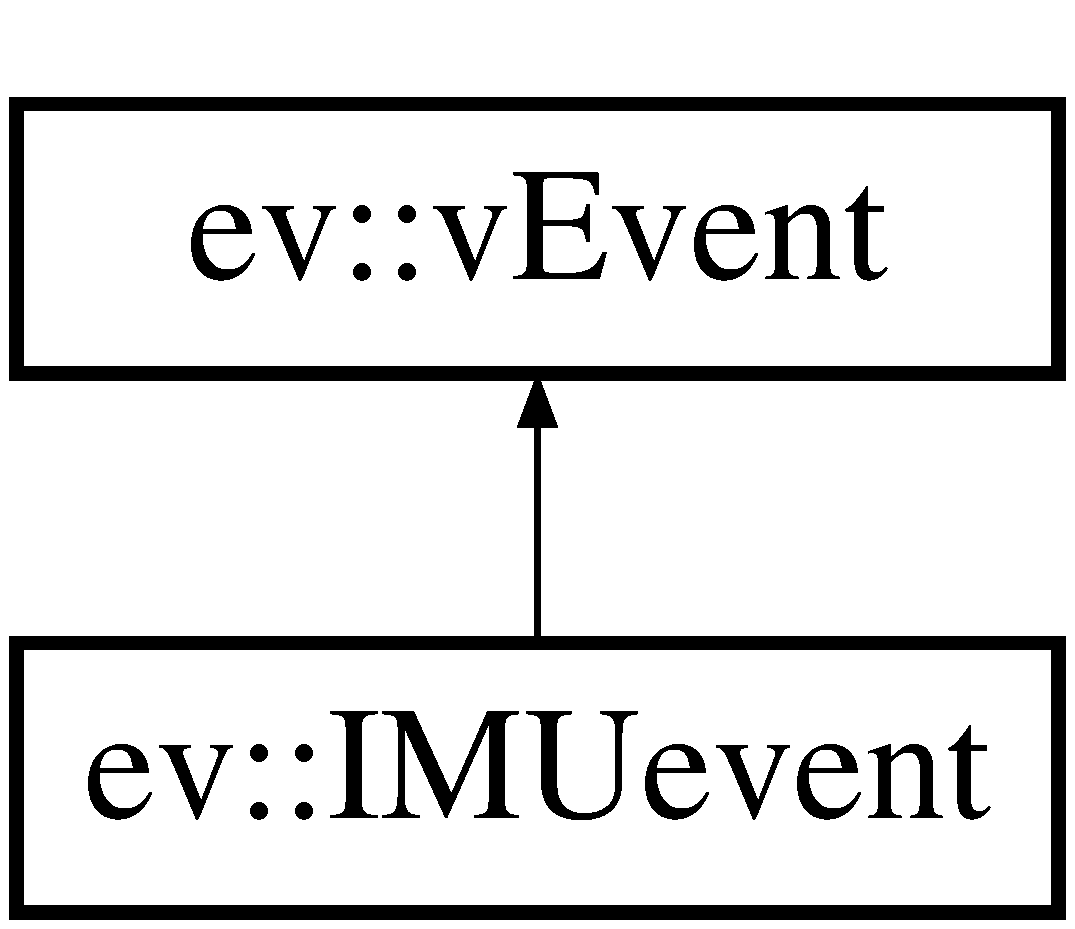
\includegraphics[height=2.000000cm]{classev_1_1IMUevent}
\end{center}
\end{figure}
\subsection*{Public Member Functions}
\begin{DoxyCompactItemize}
\item 
\mbox{\Hypertarget{classev_1_1IMUevent_aeafbaa4f2d7c17e29174ecfe3f285bfc}\label{classev_1_1IMUevent_aeafbaa4f2d7c17e29174ecfe3f285bfc}} 
{\bfseries I\+M\+Uevent} (const \hyperlink{classev_1_1vEvent}{v\+Event} \&v)
\item 
\mbox{\Hypertarget{classev_1_1IMUevent_a822d3d8bfd6dbcac987dc4eb1861d8d7}\label{classev_1_1IMUevent_a822d3d8bfd6dbcac987dc4eb1861d8d7}} 
{\bfseries I\+M\+Uevent} (const \hyperlink{classev_1_1IMUevent}{I\+M\+Uevent} \&v)
\item 
\mbox{\Hypertarget{classev_1_1IMUevent_a0dece317ec94e3f0ab1e40d50549e1c8}\label{classev_1_1IMUevent_a0dece317ec94e3f0ab1e40d50549e1c8}} 
virtual event {\bfseries clone} ()
\item 
\mbox{\Hypertarget{classev_1_1IMUevent_aff5831e99c4174bdd85689c26ce613ba}\label{classev_1_1IMUevent_aff5831e99c4174bdd85689c26ce613ba}} 
virtual void {\bfseries encode} (yarp\+::os\+::\+Bottle \&b) const
\item 
\mbox{\Hypertarget{classev_1_1IMUevent_a171f128d91d028698062060c3df4f632}\label{classev_1_1IMUevent_a171f128d91d028698062060c3df4f632}} 
virtual void {\bfseries encode} (std\+::vector$<$ int32\+\_\+t $>$ \&b, unsigned int \&pos) const
\item 
\mbox{\Hypertarget{classev_1_1IMUevent_a7fcb5f10ff8b36f9bd0f55cf50dd889d}\label{classev_1_1IMUevent_a7fcb5f10ff8b36f9bd0f55cf50dd889d}} 
virtual bool {\bfseries decode} (const yarp\+::os\+::\+Bottle \&packet, size\+\_\+t \&pos)
\item 
\mbox{\Hypertarget{classev_1_1IMUevent_a5c2c5342b24a5ed9cfb5047cb0c04a88}\label{classev_1_1IMUevent_a5c2c5342b24a5ed9cfb5047cb0c04a88}} 
virtual void {\bfseries decode} (const int32\+\_\+t $\ast$\&data)
\item 
\mbox{\Hypertarget{classev_1_1IMUevent_af4db138021c3a354726f00e1a0fad1c3}\label{classev_1_1IMUevent_af4db138021c3a354726f00e1a0fad1c3}} 
virtual yarp\+::os\+::\+Property {\bfseries get\+Content} () const
\item 
\mbox{\Hypertarget{classev_1_1IMUevent_a7d8c815714b7dea2aa7636aaddbd4ed4}\label{classev_1_1IMUevent_a7d8c815714b7dea2aa7636aaddbd4ed4}} 
virtual std\+::string {\bfseries get\+Type} () const
\item 
\mbox{\Hypertarget{classev_1_1IMUevent_a2faf0a821885f934f760b71f4053b670}\label{classev_1_1IMUevent_a2faf0a821885f934f760b71f4053b670}} 
virtual int {\bfseries get\+Channel} () const
\item 
\mbox{\Hypertarget{classev_1_1IMUevent_ae435c3d018265d56c3968bb2f1728995}\label{classev_1_1IMUevent_ae435c3d018265d56c3968bb2f1728995}} 
virtual void {\bfseries set\+Channel} (const int channel)
\end{DoxyCompactItemize}
\subsection*{Public Attributes}
\begin{DoxyCompactItemize}
\item 
\mbox{\Hypertarget{classev_1_1IMUevent_afb248b213266090a435ff4880b73f0de}\label{classev_1_1IMUevent_afb248b213266090a435ff4880b73f0de}} 
\begin{tabbing}
xx\=xx\=xx\=xx\=xx\=xx\=xx\=xx\=xx\=\kill
union \{\\
\>uint32\_t {\bfseries \_coded\_data}\\
\mbox{\Hypertarget{unionev_1_1IMUevent_1_1_0D17_a89bbdc2184dc700fff35e8caeead3527}\label{unionev_1_1IMUevent_1_1_0D17_a89bbdc2184dc700fff35e8caeead3527}} 
\>struct \{\\
\>\>int {\bfseries value}:16\\
\>\>unsigned int {\bfseries sensor}:4\\
\>\>unsigned int {\bfseries \_r1}:2\\
\>\>unsigned int {\bfseries channel}:1\\
\>\>unsigned int {\bfseries type}:1\\
\>\>unsigned int {\bfseries \_r2}:8\\
\>\} \\
\}; \\

\end{tabbing}\end{DoxyCompactItemize}
\subsection*{Static Public Attributes}
\begin{DoxyCompactItemize}
\item 
\mbox{\Hypertarget{classev_1_1IMUevent_a12ea90ffb6df46ef808eeed4df65fdf1}\label{classev_1_1IMUevent_a12ea90ffb6df46ef808eeed4df65fdf1}} 
static const std\+::string {\bfseries tag} = \char`\"{}I\+M\+US\char`\"{}
\item 
\mbox{\Hypertarget{classev_1_1IMUevent_a95583a57a83bd5fb5363d9ee7085a050}\label{classev_1_1IMUevent_a95583a57a83bd5fb5363d9ee7085a050}} 
static const unsigned int {\bfseries \+\_\+max\+\_\+value} = 32768
\end{DoxyCompactItemize}


\subsection{Detailed Description}
an event with a pixel location, camera number and polarity 

The documentation for this class was generated from the following files\+:\begin{DoxyCompactItemize}
\item 
/mnt/d/projects/event-\/driven/lib/include/event-\/driven/v\+Codec.\+h\item 
/mnt/d/projects/event-\/driven/lib/src/codecs/codec\+\_\+\+I\+M\+U\+Event.\+cpp\end{DoxyCompactItemize}

\hypertarget{classev_1_1interestDraw}{}\section{ev\+:\+:interest\+Draw Class Reference}
\label{classev_1_1interestDraw}\index{ev\+::interest\+Draw@{ev\+::interest\+Draw}}
Inheritance diagram for ev\+:\+:interest\+Draw\+:\begin{figure}[H]
\begin{center}
\leavevmode
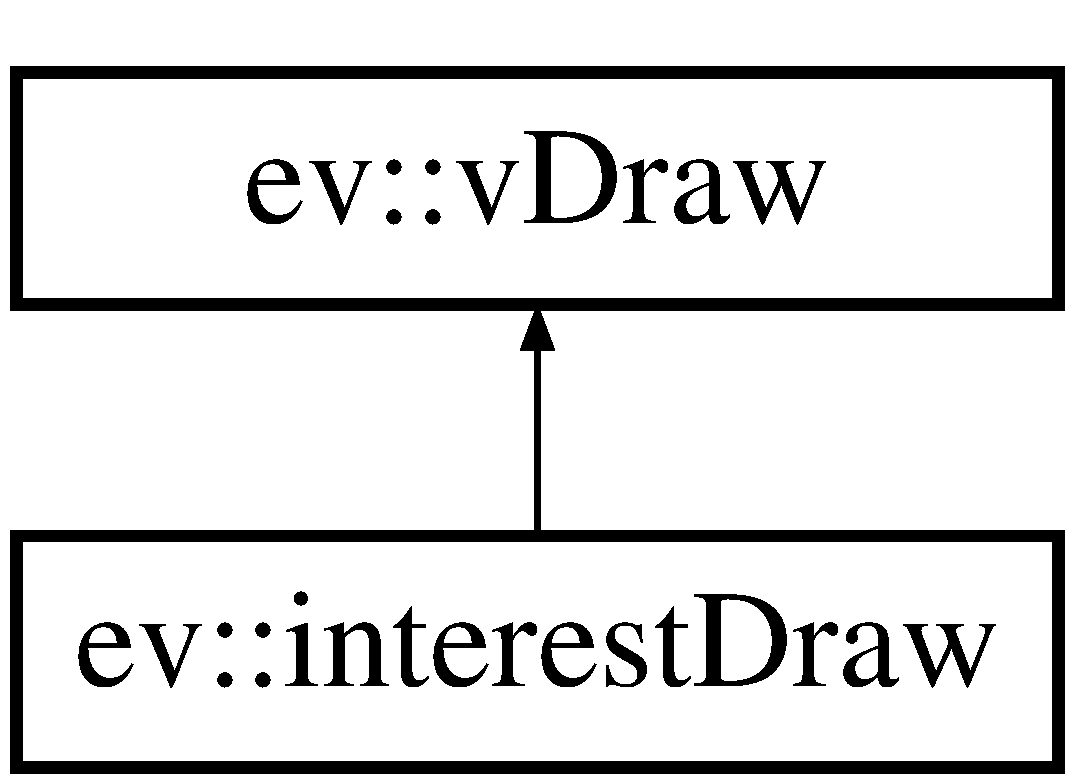
\includegraphics[height=2.000000cm]{classev_1_1interestDraw}
\end{center}
\end{figure}
\subsection*{Public Member Functions}
\begin{DoxyCompactItemize}
\item 
virtual void \hyperlink{classev_1_1interestDraw_aeca2c7248d34d6817e853aad6a254380}{draw} (cv\+::\+Mat \&image, const ev\+::v\+Queue \&e\+Set, int v\+Time)
\begin{DoxyCompactList}\small\item\em draw takes an image and overlays the new visualisation textures \end{DoxyCompactList}\item 
virtual std\+::string \hyperlink{classev_1_1interestDraw_a97dbea009b993f0d8f4b6967b2b241ad}{get\+Draw\+Type} ()
\begin{DoxyCompactList}\small\item\em get\+Tag returns the unique code for this drawing method. The arguments given on the command line must match this code exactly \end{DoxyCompactList}\item 
\mbox{\Hypertarget{classev_1_1interestDraw_a3338d66355cfdfd6c9c2b8c0ae221dff}\label{classev_1_1interestDraw_a3338d66355cfdfd6c9c2b8c0ae221dff}} 
virtual std\+::string {\bfseries get\+Event\+Type} ()
\end{DoxyCompactItemize}
\subsection*{Static Public Attributes}
\begin{DoxyCompactItemize}
\item 
\mbox{\Hypertarget{classev_1_1interestDraw_a24696c1d91d3c7866461e64e18128213}\label{classev_1_1interestDraw_a24696c1d91d3c7866461e64e18128213}} 
static const std\+::string {\bfseries drawtype} = \char`\"{}AE-\/I\+NT\char`\"{}
\end{DoxyCompactItemize}
\subsection*{Additional Inherited Members}


\subsection{Member Function Documentation}
\mbox{\Hypertarget{classev_1_1interestDraw_aeca2c7248d34d6817e853aad6a254380}\label{classev_1_1interestDraw_aeca2c7248d34d6817e853aad6a254380}} 
\index{ev\+::interest\+Draw@{ev\+::interest\+Draw}!draw@{draw}}
\index{draw@{draw}!ev\+::interest\+Draw@{ev\+::interest\+Draw}}
\subsubsection{\texorpdfstring{draw()}{draw()}}
{\footnotesize\ttfamily void ev\+::interest\+Draw\+::draw (\begin{DoxyParamCaption}\item[{cv\+::\+Mat \&}]{canvas,  }\item[{const ev\+::v\+Queue \&}]{e\+Set,  }\item[{int}]{v\+Time }\end{DoxyParamCaption})\hspace{0.3cm}{\ttfamily [virtual]}}



draw takes an image and overlays the new visualisation textures 


\begin{DoxyParams}{Parameters}
{\em canvas} & is the image which may or may not yet exist \\
\hline
{\em e\+Set} & is the set of events which could possibly be drawn \\
\hline
\end{DoxyParams}


Implements \hyperlink{classev_1_1vDraw_af1eee5dcdf3b4cfee6a3024e5cd706f8}{ev\+::v\+Draw}.

\mbox{\Hypertarget{classev_1_1interestDraw_a97dbea009b993f0d8f4b6967b2b241ad}\label{classev_1_1interestDraw_a97dbea009b993f0d8f4b6967b2b241ad}} 
\index{ev\+::interest\+Draw@{ev\+::interest\+Draw}!get\+Draw\+Type@{get\+Draw\+Type}}
\index{get\+Draw\+Type@{get\+Draw\+Type}!ev\+::interest\+Draw@{ev\+::interest\+Draw}}
\subsubsection{\texorpdfstring{get\+Draw\+Type()}{getDrawType()}}
{\footnotesize\ttfamily std\+::string ev\+::interest\+Draw\+::get\+Draw\+Type (\begin{DoxyParamCaption}{ }\end{DoxyParamCaption})\hspace{0.3cm}{\ttfamily [virtual]}}



get\+Tag returns the unique code for this drawing method. The arguments given on the command line must match this code exactly 

\begin{DoxyReturn}{Returns}
the tag code 
\end{DoxyReturn}


Implements \hyperlink{classev_1_1vDraw_ac01381befeffef2b930cbceb28b18a28}{ev\+::v\+Draw}.



The documentation for this class was generated from the following files\+:\begin{DoxyCompactItemize}
\item 
/mnt/d/projects/event-\/driven/lib/include/event-\/driven/v\+Draw.\+h\item 
/mnt/d/projects/event-\/driven/lib/src/v\+Draw\+\_\+basic.\+cpp\end{DoxyCompactItemize}

\hypertarget{classev_1_1isoDraw}{}\section{ev\+:\+:iso\+Draw Class Reference}
\label{classev_1_1isoDraw}\index{ev\+::iso\+Draw@{ev\+::iso\+Draw}}
Inheritance diagram for ev\+:\+:iso\+Draw\+:\begin{figure}[H]
\begin{center}
\leavevmode
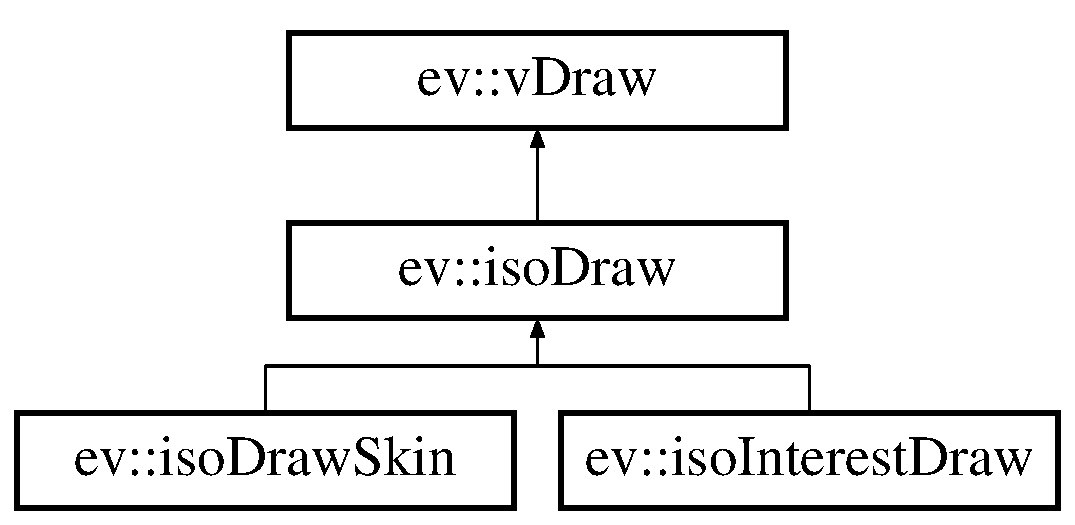
\includegraphics[height=3.000000cm]{classev_1_1isoDraw}
\end{center}
\end{figure}
\subsection*{Public Member Functions}
\begin{DoxyCompactItemize}
\item 
\mbox{\Hypertarget{classev_1_1isoDraw_a8a59ea1dc5d3ceba63edc7812b57cc8b}\label{classev_1_1isoDraw_a8a59ea1dc5d3ceba63edc7812b57cc8b}} 
void {\bfseries initialise} ()
\item 
virtual void \hyperlink{classev_1_1isoDraw_ad481b618ae2d08664481ffc4b3c4dd95}{draw} (cv\+::\+Mat \&image, const ev\+::v\+Queue \&e\+Set, int v\+Time)
\begin{DoxyCompactList}\small\item\em draw takes an image and overlays the new visualisation textures \end{DoxyCompactList}\item 
virtual std\+::string \hyperlink{classev_1_1isoDraw_abd32cc393e5489ee97b5a8b94e6dd88d}{get\+Draw\+Type} ()
\begin{DoxyCompactList}\small\item\em get\+Tag returns the unique code for this drawing method. The arguments given on the command line must match this code exactly \end{DoxyCompactList}\item 
\mbox{\Hypertarget{classev_1_1isoDraw_a65bb091100e7f29b9268d9163af675d9}\label{classev_1_1isoDraw_a65bb091100e7f29b9268d9163af675d9}} 
virtual std\+::string {\bfseries get\+Event\+Type} ()
\end{DoxyCompactItemize}
\subsection*{Static Public Attributes}
\begin{DoxyCompactItemize}
\item 
\mbox{\Hypertarget{classev_1_1isoDraw_af2ab4661d476d7fb42f3208165f42e0c}\label{classev_1_1isoDraw_af2ab4661d476d7fb42f3208165f42e0c}} 
static const std\+::string {\bfseries drawtype} = \char`\"{}I\+SO\char`\"{}
\end{DoxyCompactItemize}
\subsection*{Protected Member Functions}
\begin{DoxyCompactItemize}
\item 
\mbox{\Hypertarget{classev_1_1isoDraw_a9e4a4d519846970a5d0f12af596a7188}\label{classev_1_1isoDraw_a9e4a4d519846970a5d0f12af596a7188}} 
void {\bfseries pttr} (int \&x, int \&y, int \&z)
\end{DoxyCompactItemize}
\subsection*{Protected Attributes}
\begin{DoxyCompactItemize}
\item 
\mbox{\Hypertarget{classev_1_1isoDraw_aa2e02ca38ca08436fed9710f16a68cc0}\label{classev_1_1isoDraw_aa2e02ca38ca08436fed9710f16a68cc0}} 
double {\bfseries thetaY}
\item 
\mbox{\Hypertarget{classev_1_1isoDraw_a84f3c0bfdeeaa5d87e34bb2b515c8f68}\label{classev_1_1isoDraw_a84f3c0bfdeeaa5d87e34bb2b515c8f68}} 
double {\bfseries thetaX}
\item 
\mbox{\Hypertarget{classev_1_1isoDraw_a7bd0a4b981347fd910ef6b1105a1e44c}\label{classev_1_1isoDraw_a7bd0a4b981347fd910ef6b1105a1e44c}} 
double {\bfseries CY}
\item 
\mbox{\Hypertarget{classev_1_1isoDraw_a8bc247333b8bf395ef587da07e91e6c1}\label{classev_1_1isoDraw_a8bc247333b8bf395ef587da07e91e6c1}} 
double {\bfseries SY}
\item 
\mbox{\Hypertarget{classev_1_1isoDraw_a04de977fa3e40414ef08261bbce7d625}\label{classev_1_1isoDraw_a04de977fa3e40414ef08261bbce7d625}} 
double {\bfseries CX}
\item 
\mbox{\Hypertarget{classev_1_1isoDraw_a7bb0a3450b029f16162c3b2384fdcdbb}\label{classev_1_1isoDraw_a7bb0a3450b029f16162c3b2384fdcdbb}} 
double {\bfseries SX}
\item 
\mbox{\Hypertarget{classev_1_1isoDraw_a581e58c379835002d7118d07b051b825}\label{classev_1_1isoDraw_a581e58c379835002d7118d07b051b825}} 
double {\bfseries ts\+\_\+to\+\_\+axis}
\item 
\mbox{\Hypertarget{classev_1_1isoDraw_a817091f39e3c95e92064527c22e239f1}\label{classev_1_1isoDraw_a817091f39e3c95e92064527c22e239f1}} 
int {\bfseries Zlimit}
\item 
\mbox{\Hypertarget{classev_1_1isoDraw_a19bb2e090dffb88145fbd976064a1438}\label{classev_1_1isoDraw_a19bb2e090dffb88145fbd976064a1438}} 
int {\bfseries imagewidth}
\item 
\mbox{\Hypertarget{classev_1_1isoDraw_a7ee831adfe4c3dc13718b158a6e53ae8}\label{classev_1_1isoDraw_a7ee831adfe4c3dc13718b158a6e53ae8}} 
int {\bfseries imageheight}
\item 
\mbox{\Hypertarget{classev_1_1isoDraw_ac105029057405105a559f119b6a794db}\label{classev_1_1isoDraw_ac105029057405105a559f119b6a794db}} 
int {\bfseries imagexshift}
\item 
\mbox{\Hypertarget{classev_1_1isoDraw_a250c4a31d28b85f4151d7a92b02fc0d3}\label{classev_1_1isoDraw_a250c4a31d28b85f4151d7a92b02fc0d3}} 
int {\bfseries imageyshift}
\item 
\mbox{\Hypertarget{classev_1_1isoDraw_ae1d11e5f0c8bf377b8c90474aa9705b6}\label{classev_1_1isoDraw_ae1d11e5f0c8bf377b8c90474aa9705b6}} 
cv\+::\+Mat {\bfseries baseimage}
\end{DoxyCompactItemize}


\subsection{Member Function Documentation}
\mbox{\Hypertarget{classev_1_1isoDraw_ad481b618ae2d08664481ffc4b3c4dd95}\label{classev_1_1isoDraw_ad481b618ae2d08664481ffc4b3c4dd95}} 
\index{ev\+::iso\+Draw@{ev\+::iso\+Draw}!draw@{draw}}
\index{draw@{draw}!ev\+::iso\+Draw@{ev\+::iso\+Draw}}
\subsubsection{\texorpdfstring{draw()}{draw()}}
{\footnotesize\ttfamily void ev\+::iso\+Draw\+::draw (\begin{DoxyParamCaption}\item[{cv\+::\+Mat \&}]{canvas,  }\item[{const ev\+::v\+Queue \&}]{e\+Set,  }\item[{int}]{v\+Time }\end{DoxyParamCaption})\hspace{0.3cm}{\ttfamily [virtual]}}



draw takes an image and overlays the new visualisation textures 


\begin{DoxyParams}{Parameters}
{\em canvas} & is the image which may or may not yet exist \\
\hline
{\em e\+Set} & is the set of events which could possibly be drawn \\
\hline
\end{DoxyParams}


Implements \hyperlink{classev_1_1vDraw_af1eee5dcdf3b4cfee6a3024e5cd706f8}{ev\+::v\+Draw}.



Reimplemented in \hyperlink{classev_1_1isoDrawSkin_a2d4ed05b06bea443974f5b07a4d69374}{ev\+::iso\+Draw\+Skin}, and \hyperlink{classev_1_1isoInterestDraw_a3276f946c09d4cd0009f8379ea24d409}{ev\+::iso\+Interest\+Draw}.

\mbox{\Hypertarget{classev_1_1isoDraw_abd32cc393e5489ee97b5a8b94e6dd88d}\label{classev_1_1isoDraw_abd32cc393e5489ee97b5a8b94e6dd88d}} 
\index{ev\+::iso\+Draw@{ev\+::iso\+Draw}!get\+Draw\+Type@{get\+Draw\+Type}}
\index{get\+Draw\+Type@{get\+Draw\+Type}!ev\+::iso\+Draw@{ev\+::iso\+Draw}}
\subsubsection{\texorpdfstring{get\+Draw\+Type()}{getDrawType()}}
{\footnotesize\ttfamily std\+::string ev\+::iso\+Draw\+::get\+Draw\+Type (\begin{DoxyParamCaption}{ }\end{DoxyParamCaption})\hspace{0.3cm}{\ttfamily [virtual]}}



get\+Tag returns the unique code for this drawing method. The arguments given on the command line must match this code exactly 

\begin{DoxyReturn}{Returns}
the tag code 
\end{DoxyReturn}


Implements \hyperlink{classev_1_1vDraw_ac01381befeffef2b930cbceb28b18a28}{ev\+::v\+Draw}.



Reimplemented in \hyperlink{classev_1_1isoDrawSkin_a9f1bce77ba050a37dfe151e2246779bc}{ev\+::iso\+Draw\+Skin}, and \hyperlink{classev_1_1isoInterestDraw_a93b2142d5652f725e21d34fedde103df}{ev\+::iso\+Interest\+Draw}.



The documentation for this class was generated from the following files\+:\begin{DoxyCompactItemize}
\item 
/mnt/d/projects/event-\/driven/lib/include/event-\/driven/v\+Draw.\+h\item 
/mnt/d/projects/event-\/driven/lib/src/v\+Draw\+\_\+\+I\+S\+O.\+cpp\end{DoxyCompactItemize}

\hypertarget{classev_1_1isoDrawSkin}{}\section{ev\+:\+:iso\+Draw\+Skin Class Reference}
\label{classev_1_1isoDrawSkin}\index{ev\+::iso\+Draw\+Skin@{ev\+::iso\+Draw\+Skin}}
Inheritance diagram for ev\+:\+:iso\+Draw\+Skin\+:\begin{figure}[H]
\begin{center}
\leavevmode
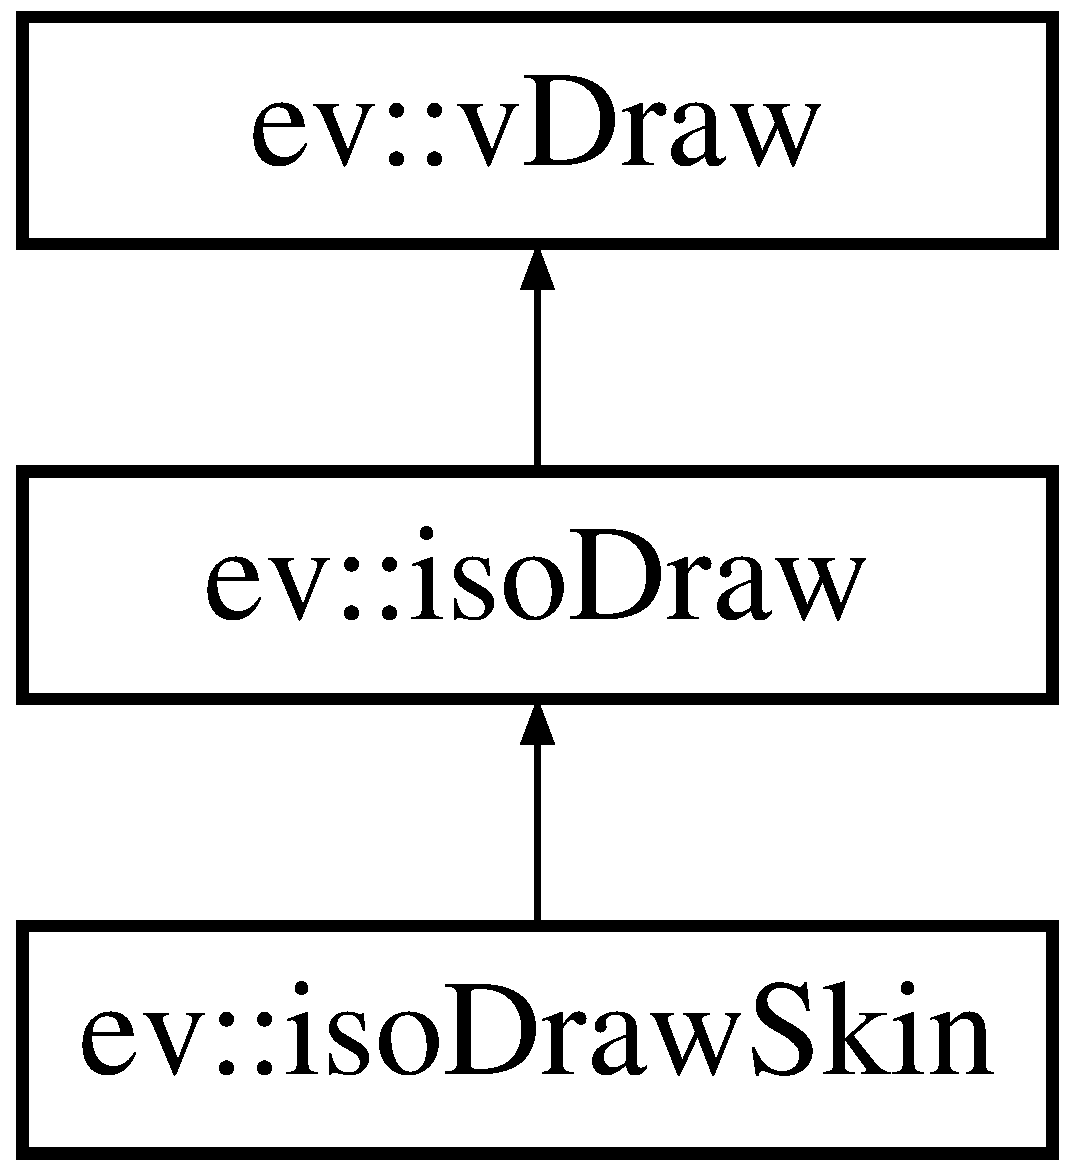
\includegraphics[height=3.000000cm]{classev_1_1isoDrawSkin}
\end{center}
\end{figure}
\subsection*{Public Member Functions}
\begin{DoxyCompactItemize}
\item 
\mbox{\Hypertarget{classev_1_1isoDrawSkin_a529da5b85b8c7e304baef5aa9e6a9d7b}\label{classev_1_1isoDrawSkin_a529da5b85b8c7e304baef5aa9e6a9d7b}} 
void {\bfseries initialise} ()
\item 
virtual void \hyperlink{classev_1_1isoDrawSkin_a2d4ed05b06bea443974f5b07a4d69374}{draw} (cv\+::\+Mat \&image, const ev\+::v\+Queue \&e\+Set, int v\+Time)
\begin{DoxyCompactList}\small\item\em draw takes an image and overlays the new visualisation textures \end{DoxyCompactList}\item 
virtual std\+::string \hyperlink{classev_1_1isoDrawSkin_a9f1bce77ba050a37dfe151e2246779bc}{get\+Draw\+Type} ()
\begin{DoxyCompactList}\small\item\em get\+Tag returns the unique code for this drawing method. The arguments given on the command line must match this code exactly \end{DoxyCompactList}\item 
\mbox{\Hypertarget{classev_1_1isoDrawSkin_acb0ea9dac4dbb4e3802646cab7239c16}\label{classev_1_1isoDrawSkin_acb0ea9dac4dbb4e3802646cab7239c16}} 
virtual std\+::string {\bfseries get\+Event\+Type} ()
\end{DoxyCompactItemize}
\subsection*{Static Public Attributes}
\begin{DoxyCompactItemize}
\item 
\mbox{\Hypertarget{classev_1_1isoDrawSkin_a3e5828dce741f4b4d329159cecc11093}\label{classev_1_1isoDrawSkin_a3e5828dce741f4b4d329159cecc11093}} 
static const std\+::string {\bfseries drawtype} = \char`\"{}I\+S\+O\+S\+K\+IN\char`\"{}
\end{DoxyCompactItemize}
\subsection*{Additional Inherited Members}


\subsection{Member Function Documentation}
\mbox{\Hypertarget{classev_1_1isoDrawSkin_a2d4ed05b06bea443974f5b07a4d69374}\label{classev_1_1isoDrawSkin_a2d4ed05b06bea443974f5b07a4d69374}} 
\index{ev\+::iso\+Draw\+Skin@{ev\+::iso\+Draw\+Skin}!draw@{draw}}
\index{draw@{draw}!ev\+::iso\+Draw\+Skin@{ev\+::iso\+Draw\+Skin}}
\subsubsection{\texorpdfstring{draw()}{draw()}}
{\footnotesize\ttfamily void ev\+::iso\+Draw\+Skin\+::draw (\begin{DoxyParamCaption}\item[{cv\+::\+Mat \&}]{canvas,  }\item[{const ev\+::v\+Queue \&}]{e\+Set,  }\item[{int}]{v\+Time }\end{DoxyParamCaption})\hspace{0.3cm}{\ttfamily [virtual]}}



draw takes an image and overlays the new visualisation textures 


\begin{DoxyParams}{Parameters}
{\em canvas} & is the image which may or may not yet exist \\
\hline
{\em e\+Set} & is the set of events which could possibly be drawn \\
\hline
\end{DoxyParams}


Reimplemented from \hyperlink{classev_1_1isoDraw_ad481b618ae2d08664481ffc4b3c4dd95}{ev\+::iso\+Draw}.

\mbox{\Hypertarget{classev_1_1isoDrawSkin_a9f1bce77ba050a37dfe151e2246779bc}\label{classev_1_1isoDrawSkin_a9f1bce77ba050a37dfe151e2246779bc}} 
\index{ev\+::iso\+Draw\+Skin@{ev\+::iso\+Draw\+Skin}!get\+Draw\+Type@{get\+Draw\+Type}}
\index{get\+Draw\+Type@{get\+Draw\+Type}!ev\+::iso\+Draw\+Skin@{ev\+::iso\+Draw\+Skin}}
\subsubsection{\texorpdfstring{get\+Draw\+Type()}{getDrawType()}}
{\footnotesize\ttfamily std\+::string ev\+::iso\+Draw\+Skin\+::get\+Draw\+Type (\begin{DoxyParamCaption}{ }\end{DoxyParamCaption})\hspace{0.3cm}{\ttfamily [virtual]}}



get\+Tag returns the unique code for this drawing method. The arguments given on the command line must match this code exactly 

\begin{DoxyReturn}{Returns}
the tag code 
\end{DoxyReturn}


Reimplemented from \hyperlink{classev_1_1isoDraw_abd32cc393e5489ee97b5a8b94e6dd88d}{ev\+::iso\+Draw}.



The documentation for this class was generated from the following files\+:\begin{DoxyCompactItemize}
\item 
/mnt/d/projects/event-\/driven/lib/include/event-\/driven/v\+Draw\+Skin.\+h\item 
/mnt/d/projects/event-\/driven/lib/src/v\+Draw\+\_\+skin.\+cpp\end{DoxyCompactItemize}

\hypertarget{classev_1_1isoInterestDraw}{}\section{ev\+:\+:iso\+Interest\+Draw Class Reference}
\label{classev_1_1isoInterestDraw}\index{ev\+::iso\+Interest\+Draw@{ev\+::iso\+Interest\+Draw}}
Inheritance diagram for ev\+:\+:iso\+Interest\+Draw\+:\begin{figure}[H]
\begin{center}
\leavevmode
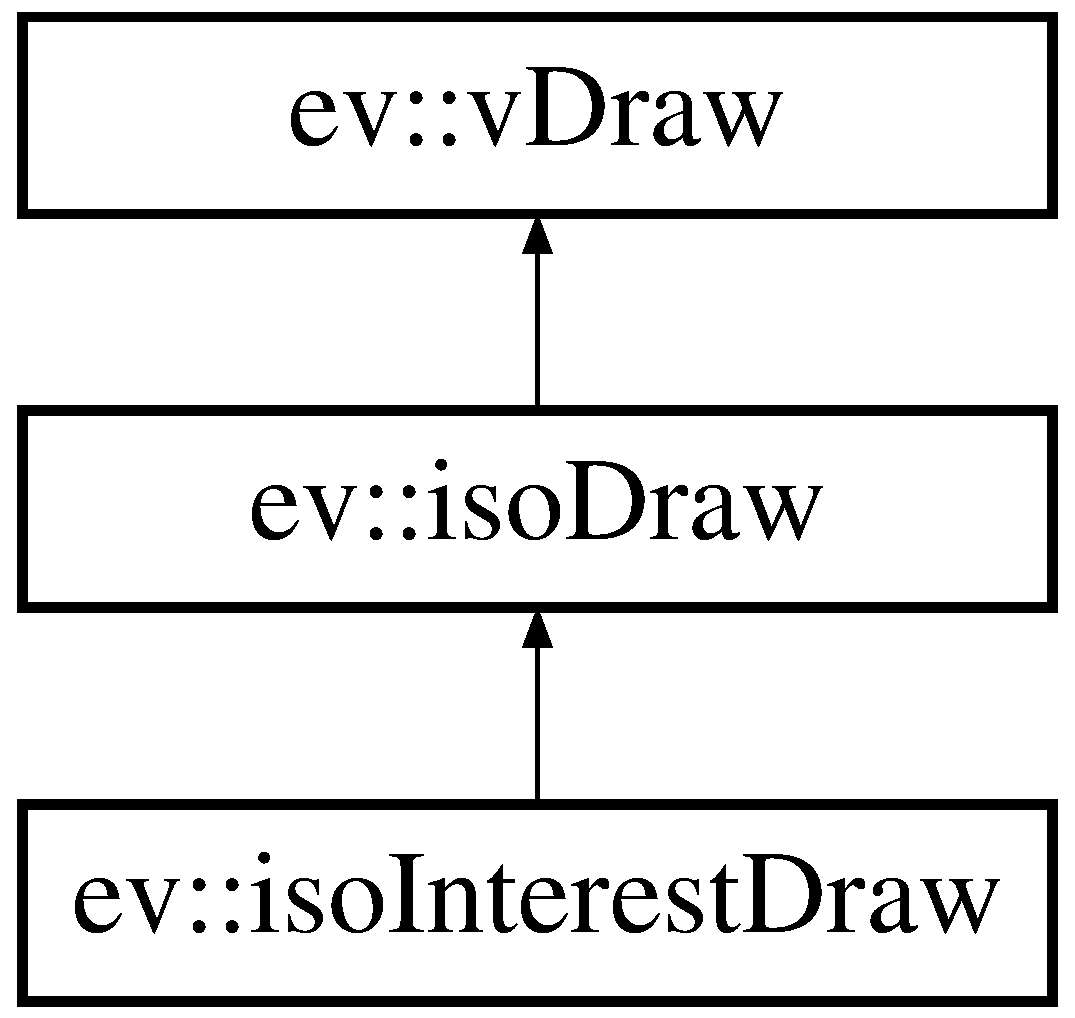
\includegraphics[height=3.000000cm]{classev_1_1isoInterestDraw}
\end{center}
\end{figure}
\subsection*{Public Member Functions}
\begin{DoxyCompactItemize}
\item 
virtual void \hyperlink{classev_1_1isoInterestDraw_a3276f946c09d4cd0009f8379ea24d409}{draw} (cv\+::\+Mat \&image, const ev\+::v\+Queue \&e\+Set, int v\+Time)
\begin{DoxyCompactList}\small\item\em draw takes an image and overlays the new visualisation textures \end{DoxyCompactList}\item 
virtual std\+::string \hyperlink{classev_1_1isoInterestDraw_a93b2142d5652f725e21d34fedde103df}{get\+Draw\+Type} ()
\begin{DoxyCompactList}\small\item\em get\+Tag returns the unique code for this drawing method. The arguments given on the command line must match this code exactly \end{DoxyCompactList}\item 
\mbox{\Hypertarget{classev_1_1isoInterestDraw_afda0762c6c3679fdd541a1df1e1fc704}\label{classev_1_1isoInterestDraw_afda0762c6c3679fdd541a1df1e1fc704}} 
virtual std\+::string {\bfseries get\+Event\+Type} ()
\end{DoxyCompactItemize}
\subsection*{Static Public Attributes}
\begin{DoxyCompactItemize}
\item 
\mbox{\Hypertarget{classev_1_1isoInterestDraw_ae416884ea2511db026669634be61d0ff}\label{classev_1_1isoInterestDraw_ae416884ea2511db026669634be61d0ff}} 
static const std\+::string {\bfseries drawtype} = \char`\"{}I\+SO-\/I\+NT\char`\"{}
\end{DoxyCompactItemize}
\subsection*{Additional Inherited Members}


\subsection{Member Function Documentation}
\mbox{\Hypertarget{classev_1_1isoInterestDraw_a3276f946c09d4cd0009f8379ea24d409}\label{classev_1_1isoInterestDraw_a3276f946c09d4cd0009f8379ea24d409}} 
\index{ev\+::iso\+Interest\+Draw@{ev\+::iso\+Interest\+Draw}!draw@{draw}}
\index{draw@{draw}!ev\+::iso\+Interest\+Draw@{ev\+::iso\+Interest\+Draw}}
\subsubsection{\texorpdfstring{draw()}{draw()}}
{\footnotesize\ttfamily void ev\+::iso\+Interest\+Draw\+::draw (\begin{DoxyParamCaption}\item[{cv\+::\+Mat \&}]{canvas,  }\item[{const ev\+::v\+Queue \&}]{e\+Set,  }\item[{int}]{v\+Time }\end{DoxyParamCaption})\hspace{0.3cm}{\ttfamily [virtual]}}



draw takes an image and overlays the new visualisation textures 


\begin{DoxyParams}{Parameters}
{\em canvas} & is the image which may or may not yet exist \\
\hline
{\em e\+Set} & is the set of events which could possibly be drawn \\
\hline
\end{DoxyParams}


Reimplemented from \hyperlink{classev_1_1isoDraw_ad481b618ae2d08664481ffc4b3c4dd95}{ev\+::iso\+Draw}.

\mbox{\Hypertarget{classev_1_1isoInterestDraw_a93b2142d5652f725e21d34fedde103df}\label{classev_1_1isoInterestDraw_a93b2142d5652f725e21d34fedde103df}} 
\index{ev\+::iso\+Interest\+Draw@{ev\+::iso\+Interest\+Draw}!get\+Draw\+Type@{get\+Draw\+Type}}
\index{get\+Draw\+Type@{get\+Draw\+Type}!ev\+::iso\+Interest\+Draw@{ev\+::iso\+Interest\+Draw}}
\subsubsection{\texorpdfstring{get\+Draw\+Type()}{getDrawType()}}
{\footnotesize\ttfamily std\+::string ev\+::iso\+Interest\+Draw\+::get\+Draw\+Type (\begin{DoxyParamCaption}{ }\end{DoxyParamCaption})\hspace{0.3cm}{\ttfamily [virtual]}}



get\+Tag returns the unique code for this drawing method. The arguments given on the command line must match this code exactly 

\begin{DoxyReturn}{Returns}
the tag code 
\end{DoxyReturn}


Reimplemented from \hyperlink{classev_1_1isoDraw_abd32cc393e5489ee97b5a8b94e6dd88d}{ev\+::iso\+Draw}.



The documentation for this class was generated from the following files\+:\begin{DoxyCompactItemize}
\item 
/mnt/d/projects/event-\/driven/lib/include/event-\/driven/v\+Draw.\+h\item 
/mnt/d/projects/event-\/driven/lib/src/v\+Draw\+\_\+\+I\+S\+O.\+cpp\end{DoxyCompactItemize}

\hypertarget{classev_1_1LabelledAE}{}\section{ev\+:\+:Labelled\+AE Class Reference}
\label{classev_1_1LabelledAE}\index{ev\+::\+Labelled\+AE@{ev\+::\+Labelled\+AE}}


an \hyperlink{classev_1_1AddressEvent}{Address\+Event} with an ID or class label  




{\ttfamily \#include $<$v\+Codec.\+h$>$}

Inheritance diagram for ev\+:\+:Labelled\+AE\+:\begin{figure}[H]
\begin{center}
\leavevmode
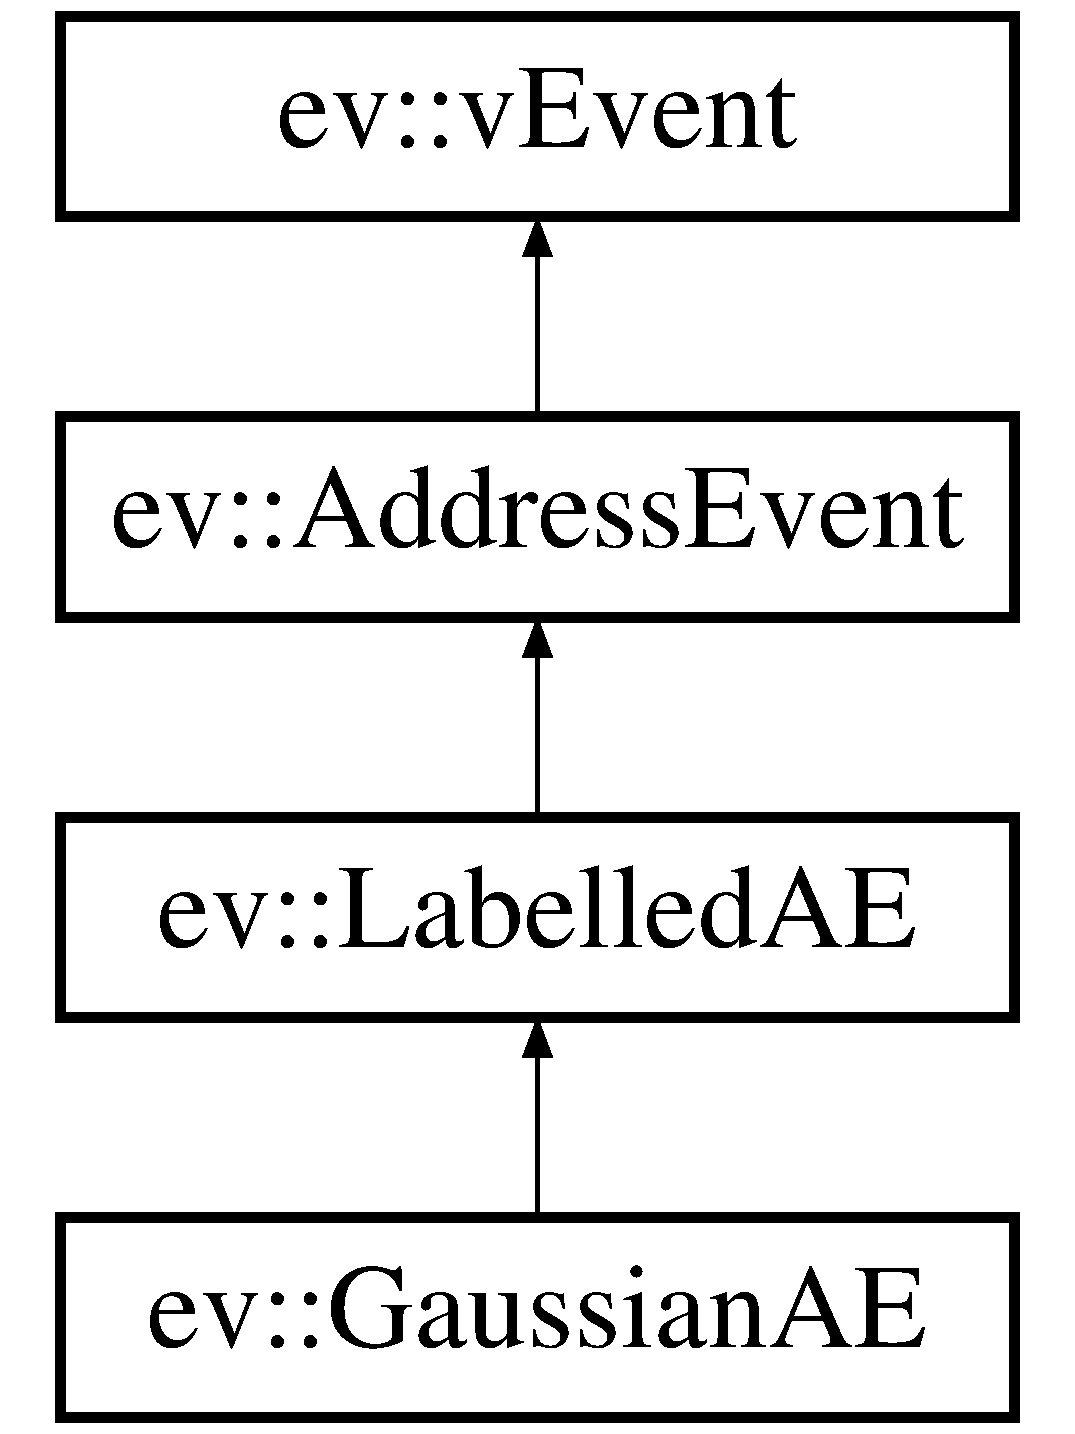
\includegraphics[height=4.000000cm]{classev_1_1LabelledAE}
\end{center}
\end{figure}
\subsection*{Public Member Functions}
\begin{DoxyCompactItemize}
\item 
\mbox{\Hypertarget{classev_1_1LabelledAE_ad9d765e87dbd81bddf3b58b7ba0f1b8a}\label{classev_1_1LabelledAE_ad9d765e87dbd81bddf3b58b7ba0f1b8a}} 
{\bfseries Labelled\+AE} (const \hyperlink{classev_1_1vEvent}{v\+Event} \&v)
\item 
\mbox{\Hypertarget{classev_1_1LabelledAE_aeca0ead752908e7c7f22aeb69b4f7e3a}\label{classev_1_1LabelledAE_aeca0ead752908e7c7f22aeb69b4f7e3a}} 
{\bfseries Labelled\+AE} (const \hyperlink{classev_1_1LabelledAE}{Labelled\+AE} \&v)
\item 
\mbox{\Hypertarget{classev_1_1LabelledAE_aad6de4f38547d2b586c333de1c247ccf}\label{classev_1_1LabelledAE_aad6de4f38547d2b586c333de1c247ccf}} 
virtual event {\bfseries clone} ()
\item 
\mbox{\Hypertarget{classev_1_1LabelledAE_a94139f3efa3348321c1abe7d83ecbec1}\label{classev_1_1LabelledAE_a94139f3efa3348321c1abe7d83ecbec1}} 
virtual void {\bfseries encode} (yarp\+::os\+::\+Bottle \&b) const
\item 
\mbox{\Hypertarget{classev_1_1LabelledAE_aaf4853cdd0109920cd5390c6fb003d9d}\label{classev_1_1LabelledAE_aaf4853cdd0109920cd5390c6fb003d9d}} 
virtual void {\bfseries encode} (std\+::vector$<$ int32\+\_\+t $>$ \&b, unsigned int \&pos) const
\item 
\mbox{\Hypertarget{classev_1_1LabelledAE_a6eb8dc1ac3a95d4fef78185d39f3fb94}\label{classev_1_1LabelledAE_a6eb8dc1ac3a95d4fef78185d39f3fb94}} 
virtual bool {\bfseries decode} (const yarp\+::os\+::\+Bottle \&packet, size\+\_\+t \&pos)
\item 
\mbox{\Hypertarget{classev_1_1LabelledAE_ab29b196e5174f6de031f8dcba3810027}\label{classev_1_1LabelledAE_ab29b196e5174f6de031f8dcba3810027}} 
virtual void {\bfseries decode} (const int32\+\_\+t $\ast$\&data)
\item 
\mbox{\Hypertarget{classev_1_1LabelledAE_a4e802e80cc0d6171372352dcad220dbd}\label{classev_1_1LabelledAE_a4e802e80cc0d6171372352dcad220dbd}} 
virtual yarp\+::os\+::\+Property {\bfseries get\+Content} () const
\item 
\mbox{\Hypertarget{classev_1_1LabelledAE_afd87d52a4b0f54994713be9c99b5b139}\label{classev_1_1LabelledAE_afd87d52a4b0f54994713be9c99b5b139}} 
virtual std\+::string {\bfseries get\+Type} () const
\end{DoxyCompactItemize}
\subsection*{Public Attributes}
\begin{DoxyCompactItemize}
\item 
\mbox{\Hypertarget{classev_1_1LabelledAE_a59a295976cdf867006deea22d7cf1942}\label{classev_1_1LabelledAE_a59a295976cdf867006deea22d7cf1942}} 
int {\bfseries ID}
\end{DoxyCompactItemize}
\subsection*{Static Public Attributes}
\begin{DoxyCompactItemize}
\item 
\mbox{\Hypertarget{classev_1_1LabelledAE_a825f9f0819046248ce7f6d0af4871cec}\label{classev_1_1LabelledAE_a825f9f0819046248ce7f6d0af4871cec}} 
static const std\+::string {\bfseries tag} = \char`\"{}L\+AE\char`\"{}
\end{DoxyCompactItemize}


\subsection{Detailed Description}
an \hyperlink{classev_1_1AddressEvent}{Address\+Event} with an ID or class label 

The documentation for this class was generated from the following files\+:\begin{DoxyCompactItemize}
\item 
/mnt/d/projects/event-\/driven/lib/include/event-\/driven/v\+Codec.\+h\item 
/mnt/d/projects/event-\/driven/lib/src/codecs/codec\+\_\+\+Labelled\+A\+E.\+cpp\end{DoxyCompactItemize}

\hypertarget{classev_1_1Left__hand}{}\section{ev\+:\+:Left\+\_\+hand Class Reference}
\label{classev_1_1Left__hand}\index{ev\+::\+Left\+\_\+hand@{ev\+::\+Left\+\_\+hand}}
Inheritance diagram for ev\+:\+:Left\+\_\+hand\+:\begin{figure}[H]
\begin{center}
\leavevmode
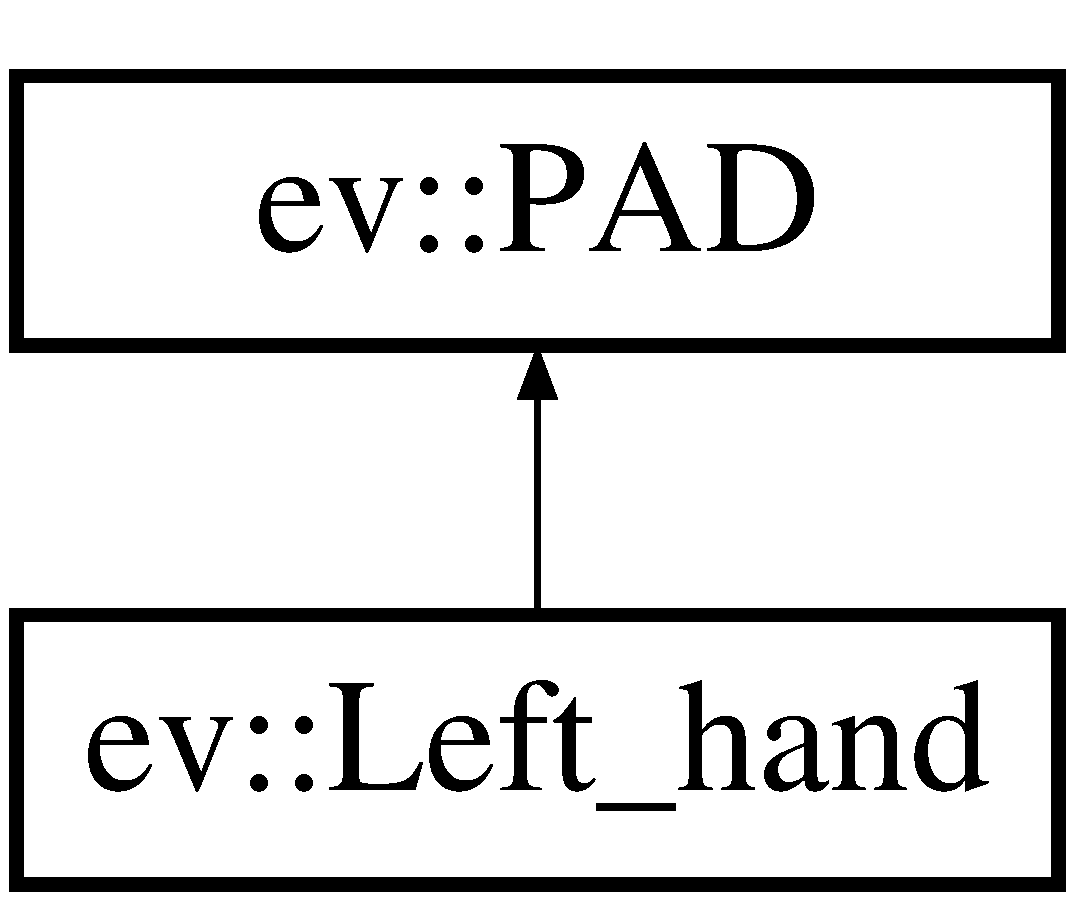
\includegraphics[height=2.000000cm]{classev_1_1Left__hand}
\end{center}
\end{figure}
\subsection*{Public Member Functions}
\begin{DoxyCompactItemize}
\item 
\mbox{\Hypertarget{classev_1_1Left__hand_aa0736fa85986f013a2e968f60553f217}\label{classev_1_1Left__hand_aa0736fa85986f013a2e968f60553f217}} 
{\bfseries Left\+\_\+hand} (int shift)
\item 
\mbox{\Hypertarget{classev_1_1Left__hand_a47162abd5620f6b2ed6fabce7a8b6060}\label{classev_1_1Left__hand_a47162abd5620f6b2ed6fabce7a8b6060}} 
void {\bfseries init\+Representative\+Taxels} (std\+::vector$<$ int $>$ taxel\+Map)
\item 
\mbox{\Hypertarget{classev_1_1Left__hand_af7d9dd729c57fa62aab4d6160e2f8f98}\label{classev_1_1Left__hand_af7d9dd729c57fa62aab4d6160e2f8f98}} 
int $\ast$ {\bfseries get\+ID} (const int index) const
\item 
\mbox{\Hypertarget{classev_1_1Left__hand_af270d362a64976a3a3c2df68af747a30}\label{classev_1_1Left__hand_af270d362a64976a3a3c2df68af747a30}} 
std\+::tuple$<$ double, double $>$ {\bfseries make\+Map} (int index) const
\end{DoxyCompactItemize}
\subsection*{Additional Inherited Members}


The documentation for this class was generated from the following file\+:\begin{DoxyCompactItemize}
\item 
/mnt/d/projects/event-\/driven/lib/include/event-\/driven/v\+Draw\+Skin.\+h\end{DoxyCompactItemize}

\hypertarget{classev_1_1lifetimeSurface}{}\section{ev\+:\+:lifetime\+Surface Class Reference}
\label{classev_1_1lifetimeSurface}\index{ev\+::lifetime\+Surface@{ev\+::lifetime\+Surface}}


a spatio-\/temporal surface storing events for a \char`\"{}lifetime\char`\"{} given by the inverse of velocity  




{\ttfamily \#include $<$v\+Window\+\_\+adv.\+h$>$}

Inheritance diagram for ev\+:\+:lifetime\+Surface\+:\begin{figure}[H]
\begin{center}
\leavevmode
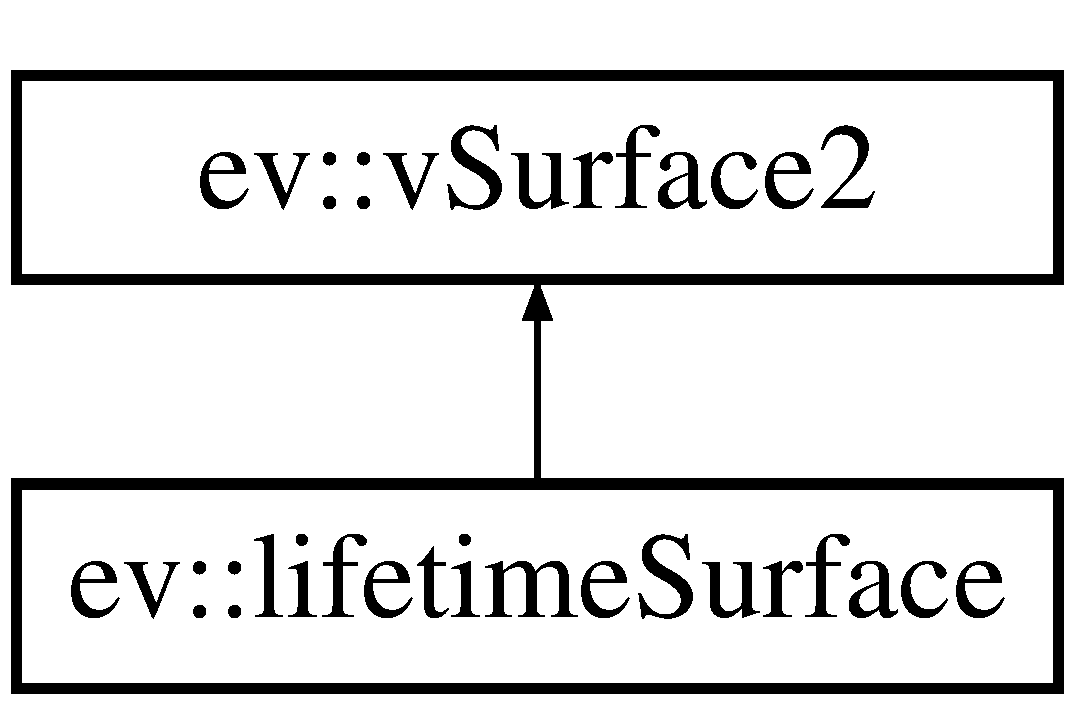
\includegraphics[height=2.000000cm]{classev_1_1lifetimeSurface}
\end{center}
\end{figure}
\subsection*{Public Member Functions}
\begin{DoxyCompactItemize}
\item 
\mbox{\Hypertarget{classev_1_1lifetimeSurface_a8276286d48b5baf2829268333f99b482}\label{classev_1_1lifetimeSurface_a8276286d48b5baf2829268333f99b482}} 
{\bfseries lifetime\+Surface} (int \hyperlink{classev_1_1vSurface2_a1aa8027816352a15d5b9bf1f26f48e76}{width}=128, int height=128)
\item 
virtual v\+Queue \hyperlink{classev_1_1lifetimeSurface_a8fce037a13281c0e46c7d660e0ea2275}{add\+Event} (event$<$$>$ to\+Add)
\begin{DoxyCompactList}\small\item\em add\+Event adds an event to the window. Also checks for expired events. \end{DoxyCompactList}\item 
\mbox{\Hypertarget{classev_1_1lifetimeSurface_a86fde904d007b5b1e5f52351bfab0b17}\label{classev_1_1lifetimeSurface_a86fde904d007b5b1e5f52351bfab0b17}} 
virtual v\+Queue {\bfseries remove\+Events} (event$<$$>$ to\+Add)
\item 
\mbox{\Hypertarget{classev_1_1lifetimeSurface_a5502828fe59c4394588acb6ffa06d445}\label{classev_1_1lifetimeSurface_a5502828fe59c4394588acb6ffa06d445}} 
virtual void {\bfseries fast\+Remove\+Events} (event$<$$>$ to\+Add)
\end{DoxyCompactItemize}
\subsection*{Additional Inherited Members}


\subsection{Detailed Description}
a spatio-\/temporal surface storing events for a \char`\"{}lifetime\char`\"{} given by the inverse of velocity 

\subsection{Member Function Documentation}
\mbox{\Hypertarget{classev_1_1lifetimeSurface_a8fce037a13281c0e46c7d660e0ea2275}\label{classev_1_1lifetimeSurface_a8fce037a13281c0e46c7d660e0ea2275}} 
\index{ev\+::lifetime\+Surface@{ev\+::lifetime\+Surface}!add\+Event@{add\+Event}}
\index{add\+Event@{add\+Event}!ev\+::lifetime\+Surface@{ev\+::lifetime\+Surface}}
\subsubsection{\texorpdfstring{add\+Event()}{addEvent()}}
{\footnotesize\ttfamily v\+Queue ev\+::lifetime\+Surface\+::add\+Event (\begin{DoxyParamCaption}\item[{event$<$$>$}]{v }\end{DoxyParamCaption})\hspace{0.3cm}{\ttfamily [virtual]}}



add\+Event adds an event to the window. Also checks for expired events. 


\begin{DoxyParams}{Parameters}
{\em event} & the event to add \\
\hline
\end{DoxyParams}


Reimplemented from \hyperlink{classev_1_1vSurface2_a6dee662976048b73d7b19e45871352da}{ev\+::v\+Surface2}.



The documentation for this class was generated from the following files\+:\begin{DoxyCompactItemize}
\item 
/mnt/d/projects/event-\/driven/lib/include/event-\/driven/v\+Window\+\_\+adv.\+h\item 
/mnt/d/projects/event-\/driven/lib/src/v\+Window\+\_\+adv.\+cpp\end{DoxyCompactItemize}

\hypertarget{classev_1_1loadMap}{}\section{ev\+:\+:load\+Map Class Reference}
\label{classev_1_1loadMap}\index{ev\+::load\+Map@{ev\+::load\+Map}}
\subsection*{Public Member Functions}
\begin{DoxyCompactItemize}
\item 
\mbox{\Hypertarget{classev_1_1loadMap_a098c0c61861210b6b3c4090f21b332e7}\label{classev_1_1loadMap_a098c0c61861210b6b3c4090f21b332e7}} 
void {\bfseries initialise} (std\+::string bodypart)
\end{DoxyCompactItemize}
\subsection*{Public Attributes}
\begin{DoxyCompactItemize}
\item 
\mbox{\Hypertarget{classev_1_1loadMap_a20d2b8bb1d0911574a906c0e43740b04}\label{classev_1_1loadMap_a20d2b8bb1d0911574a906c0e43740b04}} 
std\+::map$<$ int, std\+::tuple$<$ double, double $>$ $>$ {\bfseries pos} \{\}
\item 
\mbox{\Hypertarget{classev_1_1loadMap_aa08bacf603bd8996c10dd297fb2f0f1c}\label{classev_1_1loadMap_aa08bacf603bd8996c10dd297fb2f0f1c}} 
int {\bfseries xoffset}
\item 
\mbox{\Hypertarget{classev_1_1loadMap_a79e696c26e0a6428ce03270daef22f5d}\label{classev_1_1loadMap_a79e696c26e0a6428ce03270daef22f5d}} 
int {\bfseries yoffset}
\item 
\mbox{\Hypertarget{classev_1_1loadMap_a57681d7ce3522f2b8a10e466fb575e0f}\label{classev_1_1loadMap_a57681d7ce3522f2b8a10e466fb575e0f}} 
int {\bfseries scaling}
\item 
\mbox{\Hypertarget{classev_1_1loadMap_aef687a2418d6552d8524f69b2a8ce573}\label{classev_1_1loadMap_aef687a2418d6552d8524f69b2a8ce573}} 
int {\bfseries radius}
\item 
\mbox{\Hypertarget{classev_1_1loadMap_ab1f79cba70449cd5da4015a4ef4133d3}\label{classev_1_1loadMap_ab1f79cba70449cd5da4015a4ef4133d3}} 
int {\bfseries noise}
\item 
\mbox{\Hypertarget{classev_1_1loadMap_ad23b62a02b133aa935e30e6c5e75abf7}\label{classev_1_1loadMap_ad23b62a02b133aa935e30e6c5e75abf7}} 
int {\bfseries max\+\_\+value}
\end{DoxyCompactItemize}


The documentation for this class was generated from the following file\+:\begin{DoxyCompactItemize}
\item 
/mnt/d/projects/event-\/driven/lib/include/event-\/driven/v\+Draw\+Skin.\+h\end{DoxyCompactItemize}

\hypertarget{classev_1_1PAD}{}\section{ev\+:\+:P\+AD Class Reference}
\label{classev_1_1PAD}\index{ev\+::\+P\+AD@{ev\+::\+P\+AD}}
Inheritance diagram for ev\+:\+:P\+AD\+:\begin{figure}[H]
\begin{center}
\leavevmode
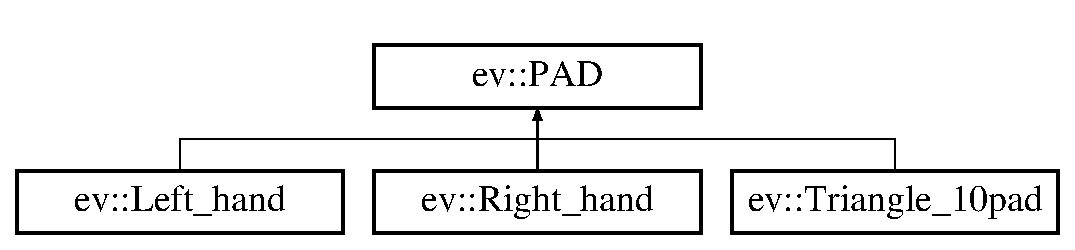
\includegraphics[height=2.000000cm]{classev_1_1PAD}
\end{center}
\end{figure}
\subsection*{Public Member Functions}
\begin{DoxyCompactItemize}
\item 
\mbox{\Hypertarget{classev_1_1PAD_a97c7228c2d197211aba3697c12971396}\label{classev_1_1PAD_a97c7228c2d197211aba3697c12971396}} 
virtual void {\bfseries init\+Representative\+Taxels} (std\+::vector$<$ int $>$ taxel\+Map)=0
\item 
\mbox{\Hypertarget{classev_1_1PAD_a46ca58b885f3508c0d2ca78694cc96cf}\label{classev_1_1PAD_a46ca58b885f3508c0d2ca78694cc96cf}} 
virtual int $\ast$ {\bfseries get\+ID} (const int index) const =0
\item 
\mbox{\Hypertarget{classev_1_1PAD_a2e2d128551f76ad51a9f77b25a6710f4}\label{classev_1_1PAD_a2e2d128551f76ad51a9f77b25a6710f4}} 
virtual std\+::tuple$<$ double, double $>$ {\bfseries make\+Map} (int ID) const =0
\item 
\mbox{\Hypertarget{classev_1_1PAD_adb5f0d48ea06f4edda3d3f7cc3e104bc}\label{classev_1_1PAD_adb5f0d48ea06f4edda3d3f7cc3e104bc}} 
void {\bfseries get\+\_\+data} (int id, double x, double y, double orientation, double gain, int mirror, int layout\+Num)
\end{DoxyCompactItemize}
\subsection*{Public Attributes}
\begin{DoxyCompactItemize}
\item 
\mbox{\Hypertarget{classev_1_1PAD_a9091308d3c2f3f098b784891c4439216}\label{classev_1_1PAD_a9091308d3c2f3f098b784891c4439216}} 
int {\bfseries xoffset} \{0\}
\item 
\mbox{\Hypertarget{classev_1_1PAD_a817c926d6b55ff09b84f6757310d5d82}\label{classev_1_1PAD_a817c926d6b55ff09b84f6757310d5d82}} 
int {\bfseries yoffset} \{0\}
\item 
\mbox{\Hypertarget{classev_1_1PAD_a0aef1dfdf94d229d889abef277800b42}\label{classev_1_1PAD_a0aef1dfdf94d229d889abef277800b42}} 
int {\bfseries scaling} \{4\}
\item 
\mbox{\Hypertarget{classev_1_1PAD_ade492e537a0159cb47c07d9da53694a1}\label{classev_1_1PAD_ade492e537a0159cb47c07d9da53694a1}} 
int {\bfseries radius} \{6\}
\item 
\mbox{\Hypertarget{classev_1_1PAD_aed64657855e265d0fca71102bb716768}\label{classev_1_1PAD_aed64657855e265d0fca71102bb716768}} 
int {\bfseries noise} \{2500\}
\item 
\mbox{\Hypertarget{classev_1_1PAD_a4c080b39fe66cb40d0975ac38e3f749f}\label{classev_1_1PAD_a4c080b39fe66cb40d0975ac38e3f749f}} 
int {\bfseries max\+\_\+value} \{15000\}
\item 
\mbox{\Hypertarget{classev_1_1PAD_a0bd154850385c9eeb5b3e67a66963ece}\label{classev_1_1PAD_a0bd154850385c9eeb5b3e67a66963ece}} 
std\+::map$<$ int, std\+::list$<$ unsigned int $>$ $>$ {\bfseries repr2\+Taxel\+List}
\end{DoxyCompactItemize}
\subsection*{Protected Member Functions}
\begin{DoxyCompactItemize}
\item 
\mbox{\Hypertarget{classev_1_1PAD_ae24c2e7c4e1a805fe18ba89806e032ad}\label{classev_1_1PAD_ae24c2e7c4e1a805fe18ba89806e032ad}} 
std\+::list$<$ unsigned int $>$ {\bfseries vectorof\+Int\+Equalto} (const std\+::vector$<$ int $>$ vec, const int val)
\end{DoxyCompactItemize}
\subsection*{Protected Attributes}
\begin{DoxyCompactItemize}
\item 
\mbox{\Hypertarget{classev_1_1PAD_a337eaa97ea7673ac50a85ca45b3b9f4c}\label{classev_1_1PAD_a337eaa97ea7673ac50a85ca45b3b9f4c}} 
const double {\bfseries D\+E\+G2\+R\+AD} =M\+\_\+\+PI/180.\+0
\item 
\mbox{\Hypertarget{classev_1_1PAD_aa1ef226653e839ac1a5087770cc2be7f}\label{classev_1_1PAD_aa1ef226653e839ac1a5087770cc2be7f}} 
int {\bfseries n\+Taxels}
\item 
\mbox{\Hypertarget{classev_1_1PAD_ae3afe0ce63f749f004f2a33f6f3e34d7}\label{classev_1_1PAD_ae3afe0ce63f749f004f2a33f6f3e34d7}} 
double $\ast$ {\bfseries dX} \{nullptr\}
\item 
\mbox{\Hypertarget{classev_1_1PAD_ae2c6e5d2357e40c73a48e22bd9c558a2}\label{classev_1_1PAD_ae2c6e5d2357e40c73a48e22bd9c558a2}} 
double $\ast$ {\bfseries dY} \{nullptr\}
\item 
\mbox{\Hypertarget{classev_1_1PAD_af9ca2f32dd78d1242658aa49a99b7998}\label{classev_1_1PAD_af9ca2f32dd78d1242658aa49a99b7998}} 
std\+::map$<$ int, std\+::vector$<$ double $>$ $>$ {\bfseries data}
\end{DoxyCompactItemize}


The documentation for this class was generated from the following file\+:\begin{DoxyCompactItemize}
\item 
/mnt/d/projects/event-\/driven/lib/include/event-\/driven/v\+Draw\+Skin.\+h\end{DoxyCompactItemize}

\hypertarget{classev_1_1queueAllocator}{}\section{ev\+:\+:queue\+Allocator Class Reference}
\label{classev_1_1queueAllocator}\index{ev\+::queue\+Allocator@{ev\+::queue\+Allocator}}


an asynchronous reading port that accepts v\+Bottles and decodes them  




{\ttfamily \#include $<$v\+Surface\+Handler\+Th.\+h$>$}

Inheritance diagram for ev\+:\+:queue\+Allocator\+:\begin{figure}[H]
\begin{center}
\leavevmode
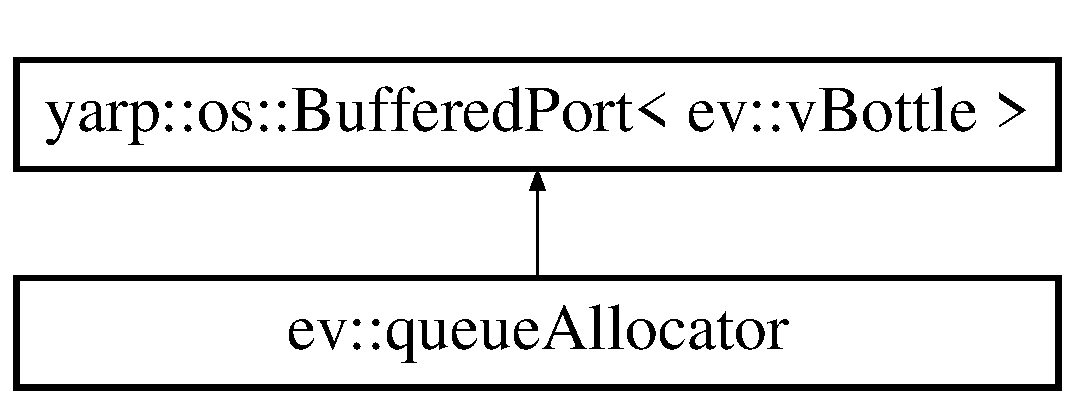
\includegraphics[height=2.000000cm]{classev_1_1queueAllocator}
\end{center}
\end{figure}
\subsection*{Public Member Functions}
\begin{DoxyCompactItemize}
\item 
\mbox{\Hypertarget{classev_1_1queueAllocator_aecc5317205f3d9d5d753dfefcb2d3228}\label{classev_1_1queueAllocator_aecc5317205f3d9d5d753dfefcb2d3228}} 
\hyperlink{classev_1_1queueAllocator_aecc5317205f3d9d5d753dfefcb2d3228}{queue\+Allocator} ()
\begin{DoxyCompactList}\small\item\em constructor \end{DoxyCompactList}\item 
\mbox{\Hypertarget{classev_1_1queueAllocator_a30954e25aa82ffd21aa513987a36bb40}\label{classev_1_1queueAllocator_a30954e25aa82ffd21aa513987a36bb40}} 
\hyperlink{classev_1_1queueAllocator_a30954e25aa82ffd21aa513987a36bb40}{$\sim$queue\+Allocator} ()
\begin{DoxyCompactList}\small\item\em desctructor \end{DoxyCompactList}\item 
\mbox{\Hypertarget{classev_1_1queueAllocator_a12ae388a8d2deb71ca5b927c3eb0a860}\label{classev_1_1queueAllocator_a12ae388a8d2deb71ca5b927c3eb0a860}} 
void \hyperlink{classev_1_1queueAllocator_a12ae388a8d2deb71ca5b927c3eb0a860}{on\+Read} (\hyperlink{classev_1_1vBottle}{ev\+::v\+Bottle} \&inputbottle)
\begin{DoxyCompactList}\small\item\em the callback decodes the incoming \hyperlink{classev_1_1vBottle}{v\+Bottle} and adds it to the list of received v\+Bottles. The yarp, and event timestamps are updated. \end{DoxyCompactList}\item 
\mbox{\Hypertarget{classev_1_1queueAllocator_aa7d2e90c0cb859b798da083eb01b486a}\label{classev_1_1queueAllocator_aa7d2e90c0cb859b798da083eb01b486a}} 
ev\+::v\+Queue $\ast$ \hyperlink{classev_1_1queueAllocator_aa7d2e90c0cb859b798da083eb01b486a}{read} (yarp\+::os\+::\+Stamp \&yarpstamp)
\begin{DoxyCompactList}\small\item\em ask for a pointer to the next v\+Queue. Blocks if no data is ready. \end{DoxyCompactList}\item 
\mbox{\Hypertarget{classev_1_1queueAllocator_a1a914bc39f534dc50a7eb2ba846753bf}\label{classev_1_1queueAllocator_a1a914bc39f534dc50a7eb2ba846753bf}} 
void \hyperlink{classev_1_1queueAllocator_a1a914bc39f534dc50a7eb2ba846753bf}{scrapQ} ()
\begin{DoxyCompactList}\small\item\em remove the most recently read v\+Queue from the list and deallocate the memory \end{DoxyCompactList}\item 
\mbox{\Hypertarget{classev_1_1queueAllocator_af6ca03ee35af1cf7dd5e2d8d8141e704}\label{classev_1_1queueAllocator_af6ca03ee35af1cf7dd5e2d8d8141e704}} 
void \hyperlink{classev_1_1queueAllocator_af6ca03ee35af1cf7dd5e2d8d8141e704}{set\+Q\+Limit} (unsigned int number\+\_\+of\+\_\+qs)
\begin{DoxyCompactList}\small\item\em set the maximum number of qs that can be stored in the buffer. A value of 0 keeps all qs. \end{DoxyCompactList}\item 
\mbox{\Hypertarget{classev_1_1queueAllocator_aa3ab79f1da7f2930811ab980347b0305}\label{classev_1_1queueAllocator_aa3ab79f1da7f2930811ab980347b0305}} 
void \hyperlink{classev_1_1queueAllocator_aa3ab79f1da7f2930811ab980347b0305}{release\+Data\+Lock} ()
\begin{DoxyCompactList}\small\item\em un\+Blocks the blocking call in get\+NextQ. Useful to ensure a graceful shutdown. No guarantee the return of get\+NextQ will be valid. \end{DoxyCompactList}\item 
\mbox{\Hypertarget{classev_1_1queueAllocator_adb785d0d33ba16522f8846da35c7ebab}\label{classev_1_1queueAllocator_adb785d0d33ba16522f8846da35c7ebab}} 
int \hyperlink{classev_1_1queueAllocator_adb785d0d33ba16522f8846da35c7ebab}{queryunprocessed} ()
\begin{DoxyCompactList}\small\item\em ask for the number of v\+Queues currently allocated. \end{DoxyCompactList}\item 
\mbox{\Hypertarget{classev_1_1queueAllocator_a557861a4f3730b4d8da7895173c6986a}\label{classev_1_1queueAllocator_a557861a4f3730b4d8da7895173c6986a}} 
unsigned int \hyperlink{classev_1_1queueAllocator_a557861a4f3730b4d8da7895173c6986a}{query\+DelayN} ()
\begin{DoxyCompactList}\small\item\em ask for the number of events in all v\+Queues. \end{DoxyCompactList}\item 
\mbox{\Hypertarget{classev_1_1queueAllocator_a439a2729d5474986977e26e63a9edf03}\label{classev_1_1queueAllocator_a439a2729d5474986977e26e63a9edf03}} 
double \hyperlink{classev_1_1queueAllocator_a439a2729d5474986977e26e63a9edf03}{query\+DelayT} ()
\begin{DoxyCompactList}\small\item\em ask for the total time spanned by all v\+Queues. \end{DoxyCompactList}\item 
\mbox{\Hypertarget{classev_1_1queueAllocator_a39005a8e9337279debe435ae26c7d6fd}\label{classev_1_1queueAllocator_a39005a8e9337279debe435ae26c7d6fd}} 
double \hyperlink{classev_1_1queueAllocator_a39005a8e9337279debe435ae26c7d6fd}{query\+Rate} ()
\begin{DoxyCompactList}\small\item\em ask for the high precision event rate \end{DoxyCompactList}\item 
\mbox{\Hypertarget{classev_1_1queueAllocator_a10282570a776a59efd302bb336109748}\label{classev_1_1queueAllocator_a10282570a776a59efd302bb336109748}} 
std\+::string {\bfseries delay\+Stat\+String} ()
\end{DoxyCompactItemize}


\subsection{Detailed Description}
an asynchronous reading port that accepts v\+Bottles and decodes them 

The documentation for this class was generated from the following file\+:\begin{DoxyCompactItemize}
\item 
/mnt/d/projects/event-\/driven/lib/include/event-\/driven/v\+Surface\+Handler\+Th.\+h\end{DoxyCompactItemize}

\hypertarget{classev_1_1rasterDraw}{}\section{ev\+:\+:raster\+Draw Class Reference}
\label{classev_1_1rasterDraw}\index{ev\+::raster\+Draw@{ev\+::raster\+Draw}}
Inheritance diagram for ev\+:\+:raster\+Draw\+:\begin{figure}[H]
\begin{center}
\leavevmode
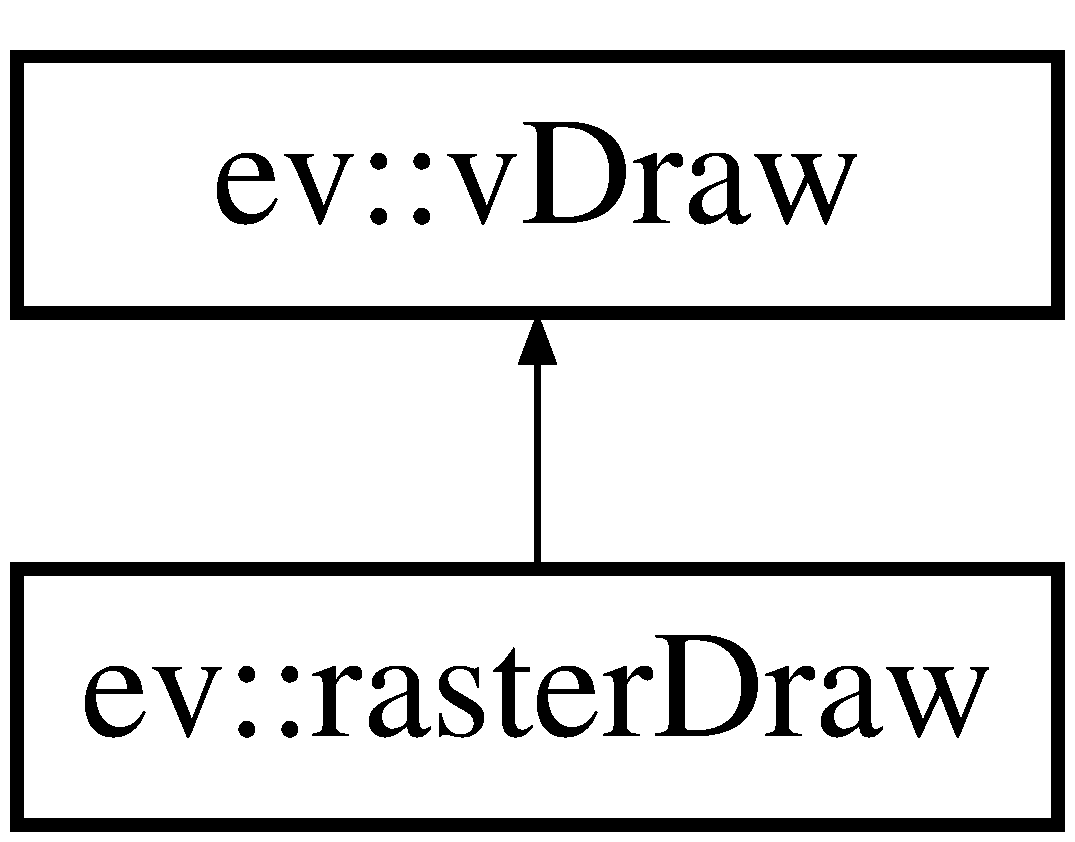
\includegraphics[height=2.000000cm]{classev_1_1rasterDraw}
\end{center}
\end{figure}
\subsection*{Public Member Functions}
\begin{DoxyCompactItemize}
\item 
\mbox{\Hypertarget{classev_1_1rasterDraw_a7b1e9d355a0c8ea0affd2fd70e77f408}\label{classev_1_1rasterDraw_a7b1e9d355a0c8ea0affd2fd70e77f408}} 
virtual void {\bfseries initialise} ()
\item 
virtual void \hyperlink{classev_1_1rasterDraw_a0cc698fe53b645a8a1ed8cdb40c8b7a9}{draw} (cv\+::\+Mat \&image, const ev\+::v\+Queue \&e\+Set, int v\+Time)
\begin{DoxyCompactList}\small\item\em draw takes an image and overlays the new visualisation textures \end{DoxyCompactList}\item 
virtual std\+::string \hyperlink{classev_1_1rasterDraw_a687569e3beafa6aa9e73e3eeaad64d59}{get\+Draw\+Type} ()
\begin{DoxyCompactList}\small\item\em get\+Tag returns the unique code for this drawing method. The arguments given on the command line must match this code exactly \end{DoxyCompactList}\item 
\mbox{\Hypertarget{classev_1_1rasterDraw_a669ab1be35fbe7f32d172380dc78553a}\label{classev_1_1rasterDraw_a669ab1be35fbe7f32d172380dc78553a}} 
virtual std\+::string {\bfseries get\+Event\+Type} ()
\end{DoxyCompactItemize}
\subsection*{Static Public Attributes}
\begin{DoxyCompactItemize}
\item 
\mbox{\Hypertarget{classev_1_1rasterDraw_a06c45585c1be282ee35e4905a9c8e9e9}\label{classev_1_1rasterDraw_a06c45585c1be282ee35e4905a9c8e9e9}} 
static const std\+::string {\bfseries drawtype} = \char`\"{}R\+A\+S\+T\+ER\char`\"{}
\end{DoxyCompactItemize}
\subsection*{Protected Attributes}
\begin{DoxyCompactItemize}
\item 
\mbox{\Hypertarget{classev_1_1rasterDraw_a5514c37ed65ebed9c8214be62e7d57ad}\label{classev_1_1rasterDraw_a5514c37ed65ebed9c8214be62e7d57ad}} 
float {\bfseries time\+\_\+scaler}
\item 
\mbox{\Hypertarget{classev_1_1rasterDraw_a87ff52dc9731f95dad3873573fcd8681}\label{classev_1_1rasterDraw_a87ff52dc9731f95dad3873573fcd8681}} 
unsigned int {\bfseries num\+\_\+neurons}
\end{DoxyCompactItemize}


\subsection{Member Function Documentation}
\mbox{\Hypertarget{classev_1_1rasterDraw_a0cc698fe53b645a8a1ed8cdb40c8b7a9}\label{classev_1_1rasterDraw_a0cc698fe53b645a8a1ed8cdb40c8b7a9}} 
\index{ev\+::raster\+Draw@{ev\+::raster\+Draw}!draw@{draw}}
\index{draw@{draw}!ev\+::raster\+Draw@{ev\+::raster\+Draw}}
\subsubsection{\texorpdfstring{draw()}{draw()}}
{\footnotesize\ttfamily void ev\+::raster\+Draw\+::draw (\begin{DoxyParamCaption}\item[{cv\+::\+Mat \&}]{canvas,  }\item[{const ev\+::v\+Queue \&}]{e\+Set,  }\item[{int}]{v\+Time }\end{DoxyParamCaption})\hspace{0.3cm}{\ttfamily [virtual]}}



draw takes an image and overlays the new visualisation textures 


\begin{DoxyParams}{Parameters}
{\em canvas} & is the image which may or may not yet exist \\
\hline
{\em e\+Set} & is the set of events which could possibly be drawn \\
\hline
\end{DoxyParams}


Implements \hyperlink{classev_1_1vDraw_af1eee5dcdf3b4cfee6a3024e5cd706f8}{ev\+::v\+Draw}.

\mbox{\Hypertarget{classev_1_1rasterDraw_a687569e3beafa6aa9e73e3eeaad64d59}\label{classev_1_1rasterDraw_a687569e3beafa6aa9e73e3eeaad64d59}} 
\index{ev\+::raster\+Draw@{ev\+::raster\+Draw}!get\+Draw\+Type@{get\+Draw\+Type}}
\index{get\+Draw\+Type@{get\+Draw\+Type}!ev\+::raster\+Draw@{ev\+::raster\+Draw}}
\subsubsection{\texorpdfstring{get\+Draw\+Type()}{getDrawType()}}
{\footnotesize\ttfamily std\+::string ev\+::raster\+Draw\+::get\+Draw\+Type (\begin{DoxyParamCaption}{ }\end{DoxyParamCaption})\hspace{0.3cm}{\ttfamily [virtual]}}



get\+Tag returns the unique code for this drawing method. The arguments given on the command line must match this code exactly 

\begin{DoxyReturn}{Returns}
the tag code 
\end{DoxyReturn}


Implements \hyperlink{classev_1_1vDraw_ac01381befeffef2b930cbceb28b18a28}{ev\+::v\+Draw}.



The documentation for this class was generated from the following files\+:\begin{DoxyCompactItemize}
\item 
/mnt/d/projects/event-\/driven/lib/include/event-\/driven/v\+Draw.\+h\item 
/mnt/d/projects/event-\/driven/lib/src/v\+Draw\+\_\+basic.\+cpp\end{DoxyCompactItemize}

\hypertarget{structev_1_1resolution}{}\section{ev\+:\+:resolution Struct Reference}
\label{structev_1_1resolution}\index{ev\+::resolution@{ev\+::resolution}}


an efficient structure for storing sensor resolution  




{\ttfamily \#include $<$vts\+Helper.\+h$>$}

\subsection*{Public Attributes}
\begin{DoxyCompactItemize}
\item 
\mbox{\Hypertarget{structev_1_1resolution_af63d9f023bf48b5170fbde6fac1fa60d}\label{structev_1_1resolution_af63d9f023bf48b5170fbde6fac1fa60d}} 
unsigned int {\bfseries width}\+:10
\item 
\mbox{\Hypertarget{structev_1_1resolution_ae9919e691ce05e1bbbf281dd79102ddb}\label{structev_1_1resolution_ae9919e691ce05e1bbbf281dd79102ddb}} 
unsigned int {\bfseries height}\+:10
\end{DoxyCompactItemize}


\subsection{Detailed Description}
an efficient structure for storing sensor resolution 

The documentation for this struct was generated from the following file\+:\begin{DoxyCompactItemize}
\item 
/mnt/d/projects/event-\/driven/lib/include/event-\/driven/vts\+Helper.\+h\end{DoxyCompactItemize}

\hypertarget{classev_1_1Right__hand}{}\section{ev\+:\+:Right\+\_\+hand Class Reference}
\label{classev_1_1Right__hand}\index{ev\+::\+Right\+\_\+hand@{ev\+::\+Right\+\_\+hand}}
Inheritance diagram for ev\+:\+:Right\+\_\+hand\+:\begin{figure}[H]
\begin{center}
\leavevmode
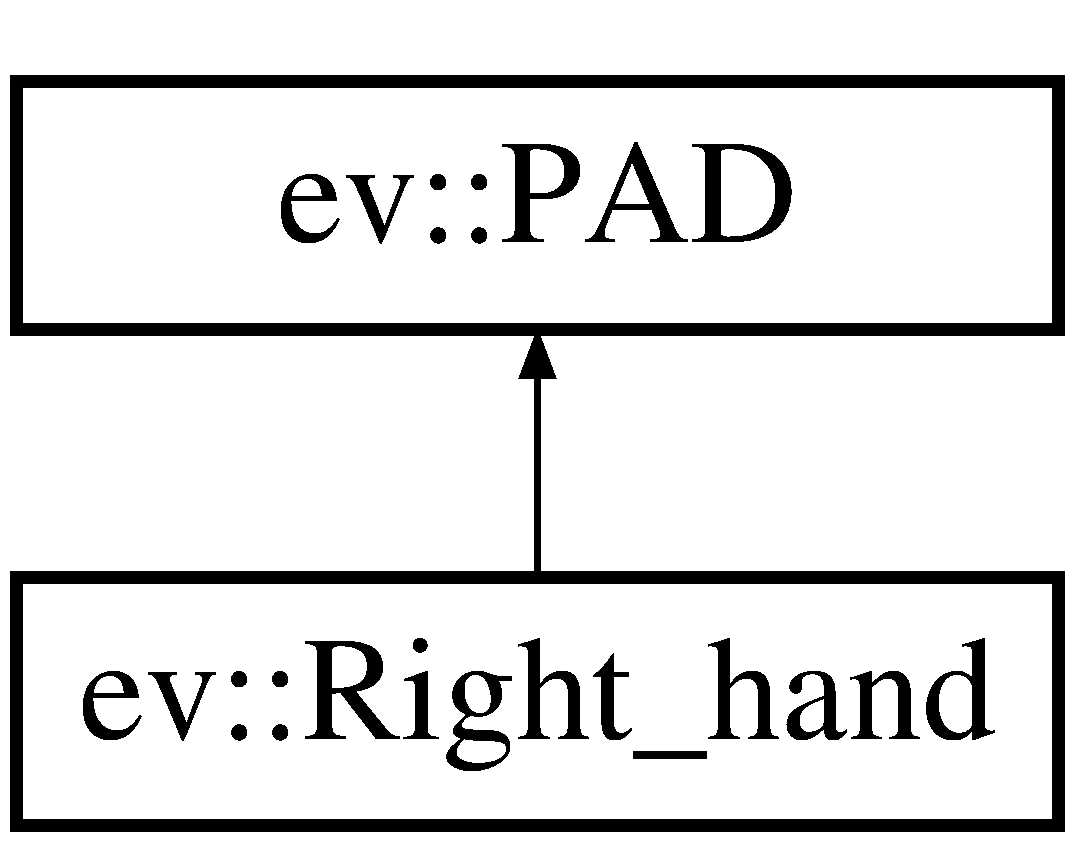
\includegraphics[height=2.000000cm]{classev_1_1Right__hand}
\end{center}
\end{figure}
\subsection*{Public Member Functions}
\begin{DoxyCompactItemize}
\item 
\mbox{\Hypertarget{classev_1_1Right__hand_ad26ab3cda248556854bf8d9073a449f7}\label{classev_1_1Right__hand_ad26ab3cda248556854bf8d9073a449f7}} 
{\bfseries Right\+\_\+hand} (int shift)
\item 
\mbox{\Hypertarget{classev_1_1Right__hand_a1c7c2dcfede67120e03eadb52b387e24}\label{classev_1_1Right__hand_a1c7c2dcfede67120e03eadb52b387e24}} 
void {\bfseries init\+Representative\+Taxels} (std\+::vector$<$ int $>$ taxel\+Map)
\item 
\mbox{\Hypertarget{classev_1_1Right__hand_a6d314e7bccd20139b5da3cf1dcf0bcc3}\label{classev_1_1Right__hand_a6d314e7bccd20139b5da3cf1dcf0bcc3}} 
int $\ast$ {\bfseries get\+ID} (const int index) const
\item 
\mbox{\Hypertarget{classev_1_1Right__hand_a1ccafa91c2d982046beeb757be83b7ad}\label{classev_1_1Right__hand_a1ccafa91c2d982046beeb757be83b7ad}} 
std\+::tuple$<$ double, double $>$ {\bfseries make\+Map} (int index) const
\end{DoxyCompactItemize}
\subsection*{Additional Inherited Members}


The documentation for this class was generated from the following file\+:\begin{DoxyCompactItemize}
\item 
/mnt/d/projects/event-\/driven/lib/include/event-\/driven/v\+Draw\+Skin.\+h\end{DoxyCompactItemize}

\hypertarget{classev_1_1skinDraw}{}\section{ev\+:\+:skin\+Draw Class Reference}
\label{classev_1_1skinDraw}\index{ev\+::skin\+Draw@{ev\+::skin\+Draw}}
Inheritance diagram for ev\+:\+:skin\+Draw\+:\begin{figure}[H]
\begin{center}
\leavevmode
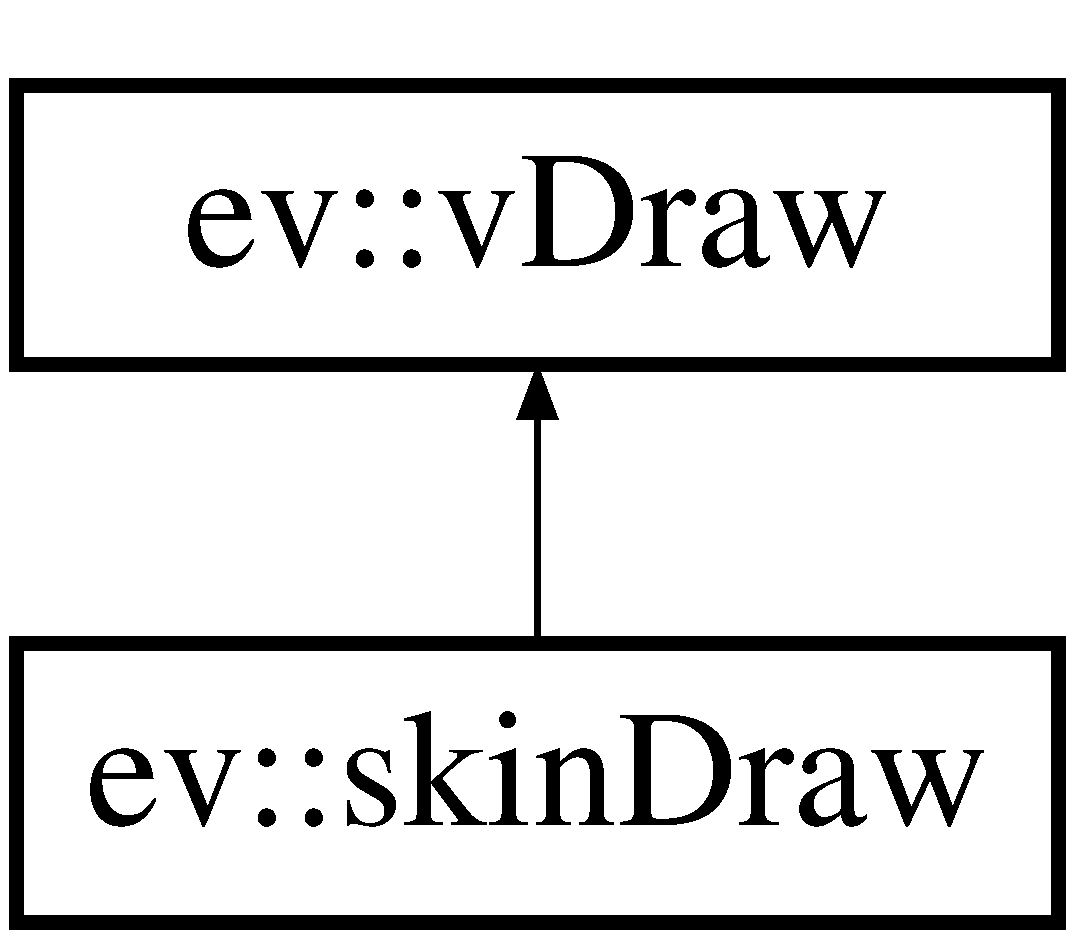
\includegraphics[height=2.000000cm]{classev_1_1skinDraw}
\end{center}
\end{figure}
\subsection*{Public Member Functions}
\begin{DoxyCompactItemize}
\item 
\mbox{\Hypertarget{classev_1_1skinDraw_ad3d3dab23e10ceafc546720fddab60e1}\label{classev_1_1skinDraw_ad3d3dab23e10ceafc546720fddab60e1}} 
void {\bfseries initialise} ()
\item 
\mbox{\Hypertarget{classev_1_1skinDraw_a0203a5fa2e0d18785c96f1d8bcacbdfd}\label{classev_1_1skinDraw_a0203a5fa2e0d18785c96f1d8bcacbdfd}} 
virtual void {\bfseries reset\+Image} (cv\+::\+Mat \&image)
\item 
virtual void \hyperlink{classev_1_1skinDraw_a4cbf578dd04c6a634c8959fea7295060}{draw} (cv\+::\+Mat \&image, const ev\+::v\+Queue \&e\+Set, int v\+Time)
\begin{DoxyCompactList}\small\item\em draw takes an image and overlays the new visualisation textures \end{DoxyCompactList}\item 
virtual std\+::string \hyperlink{classev_1_1skinDraw_a7015a083dffe5c055808c20b9372bce4}{get\+Draw\+Type} ()
\begin{DoxyCompactList}\small\item\em get\+Tag returns the unique code for this drawing method. The arguments given on the command line must match this code exactly \end{DoxyCompactList}\item 
\mbox{\Hypertarget{classev_1_1skinDraw_aa054c667234061c84ebcd94368bb5939}\label{classev_1_1skinDraw_aa054c667234061c84ebcd94368bb5939}} 
virtual std\+::string {\bfseries get\+Event\+Type} ()
\end{DoxyCompactItemize}
\subsection*{Static Public Attributes}
\begin{DoxyCompactItemize}
\item 
\mbox{\Hypertarget{classev_1_1skinDraw_a95970aec26d3174050d36bb4f15d5413}\label{classev_1_1skinDraw_a95970aec26d3174050d36bb4f15d5413}} 
static const std\+::string {\bfseries drawtype} = \char`\"{}S\+K\+IN\char`\"{}
\end{DoxyCompactItemize}
\subsection*{Additional Inherited Members}


\subsection{Member Function Documentation}
\mbox{\Hypertarget{classev_1_1skinDraw_a4cbf578dd04c6a634c8959fea7295060}\label{classev_1_1skinDraw_a4cbf578dd04c6a634c8959fea7295060}} 
\index{ev\+::skin\+Draw@{ev\+::skin\+Draw}!draw@{draw}}
\index{draw@{draw}!ev\+::skin\+Draw@{ev\+::skin\+Draw}}
\subsubsection{\texorpdfstring{draw()}{draw()}}
{\footnotesize\ttfamily void ev\+::skin\+Draw\+::draw (\begin{DoxyParamCaption}\item[{cv\+::\+Mat \&}]{canvas,  }\item[{const ev\+::v\+Queue \&}]{e\+Set,  }\item[{int}]{v\+Time }\end{DoxyParamCaption})\hspace{0.3cm}{\ttfamily [virtual]}}



draw takes an image and overlays the new visualisation textures 


\begin{DoxyParams}{Parameters}
{\em canvas} & is the image which may or may not yet exist \\
\hline
{\em e\+Set} & is the set of events which could possibly be drawn \\
\hline
\end{DoxyParams}


Implements \hyperlink{classev_1_1vDraw_af1eee5dcdf3b4cfee6a3024e5cd706f8}{ev\+::v\+Draw}.

\mbox{\Hypertarget{classev_1_1skinDraw_a7015a083dffe5c055808c20b9372bce4}\label{classev_1_1skinDraw_a7015a083dffe5c055808c20b9372bce4}} 
\index{ev\+::skin\+Draw@{ev\+::skin\+Draw}!get\+Draw\+Type@{get\+Draw\+Type}}
\index{get\+Draw\+Type@{get\+Draw\+Type}!ev\+::skin\+Draw@{ev\+::skin\+Draw}}
\subsubsection{\texorpdfstring{get\+Draw\+Type()}{getDrawType()}}
{\footnotesize\ttfamily std\+::string ev\+::skin\+Draw\+::get\+Draw\+Type (\begin{DoxyParamCaption}{ }\end{DoxyParamCaption})\hspace{0.3cm}{\ttfamily [virtual]}}



get\+Tag returns the unique code for this drawing method. The arguments given on the command line must match this code exactly 

\begin{DoxyReturn}{Returns}
the tag code 
\end{DoxyReturn}


Implements \hyperlink{classev_1_1vDraw_ac01381befeffef2b930cbceb28b18a28}{ev\+::v\+Draw}.



The documentation for this class was generated from the following files\+:\begin{DoxyCompactItemize}
\item 
/mnt/d/projects/event-\/driven/lib/include/event-\/driven/v\+Draw\+Skin.\+h\item 
/mnt/d/projects/event-\/driven/lib/src/v\+Draw\+\_\+skin.\+cpp\end{DoxyCompactItemize}

\hypertarget{classev_1_1SkinEvent}{}\section{ev\+:\+:Skin\+Event Class Reference}
\label{classev_1_1SkinEvent}\index{ev\+::\+Skin\+Event@{ev\+::\+Skin\+Event}}


an event with a taxel location, body-\/part and polarity  




{\ttfamily \#include $<$v\+Codec.\+h$>$}

Inheritance diagram for ev\+:\+:Skin\+Event\+:\begin{figure}[H]
\begin{center}
\leavevmode
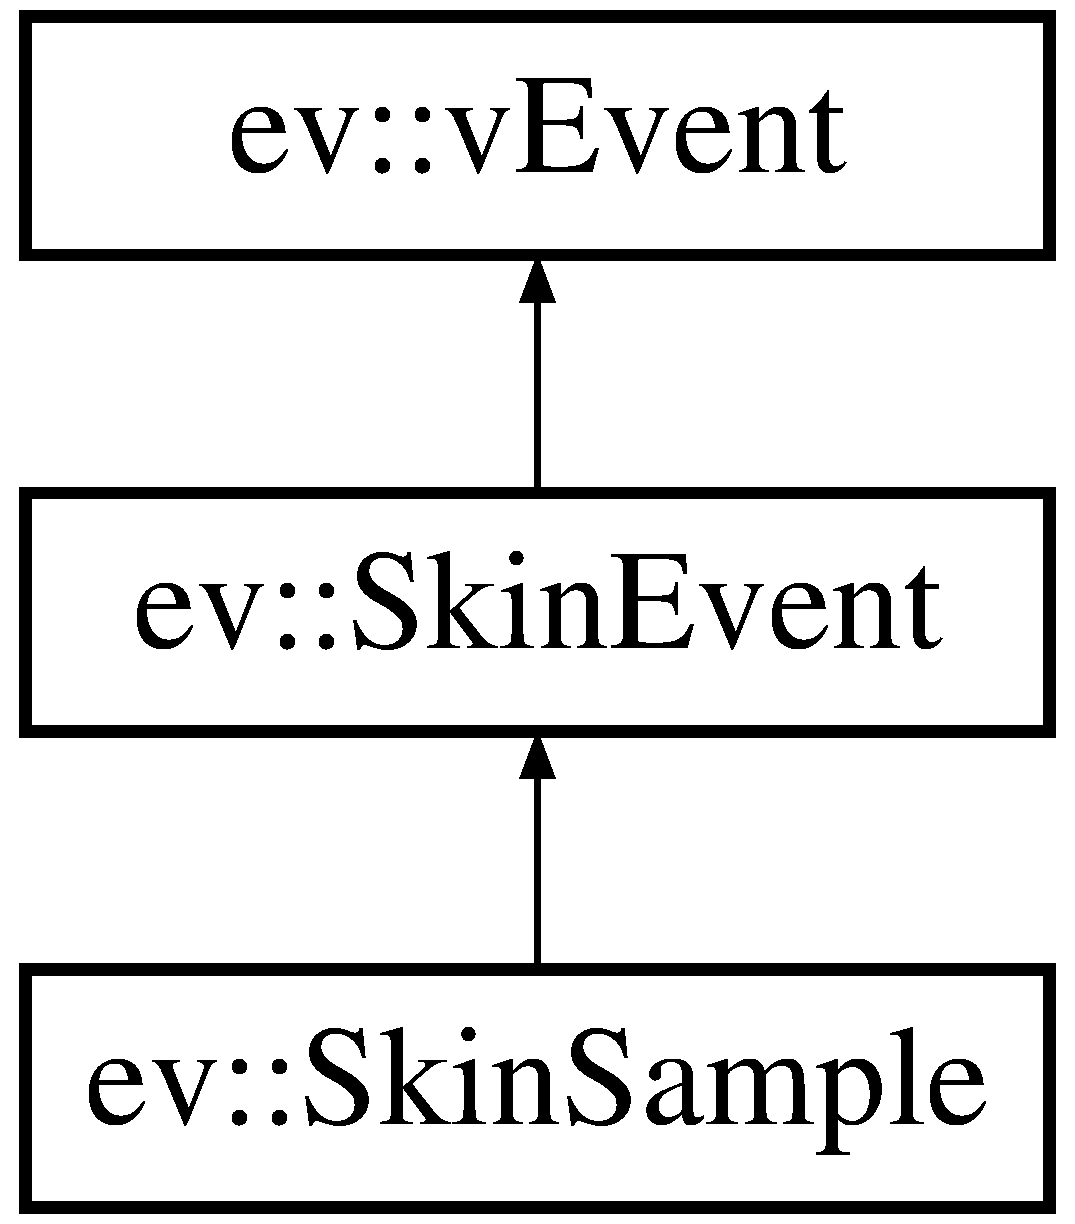
\includegraphics[height=3.000000cm]{classev_1_1SkinEvent}
\end{center}
\end{figure}
\subsection*{Public Member Functions}
\begin{DoxyCompactItemize}
\item 
\mbox{\Hypertarget{classev_1_1SkinEvent_a8921fcb24d5b22cbb4640cc78d37eb6b}\label{classev_1_1SkinEvent_a8921fcb24d5b22cbb4640cc78d37eb6b}} 
{\bfseries Skin\+Event} (const \hyperlink{classev_1_1vEvent}{v\+Event} \&v)
\item 
\mbox{\Hypertarget{classev_1_1SkinEvent_a8e8554c5d291013c572eb93723f95138}\label{classev_1_1SkinEvent_a8e8554c5d291013c572eb93723f95138}} 
{\bfseries Skin\+Event} (const \hyperlink{classev_1_1SkinEvent}{Skin\+Event} \&v)
\item 
\mbox{\Hypertarget{classev_1_1SkinEvent_a3571bc8aba54704e0f2835ab0f0a71b0}\label{classev_1_1SkinEvent_a3571bc8aba54704e0f2835ab0f0a71b0}} 
virtual event {\bfseries clone} ()
\item 
\mbox{\Hypertarget{classev_1_1SkinEvent_a5996a03de9a5711704365084ca13c410}\label{classev_1_1SkinEvent_a5996a03de9a5711704365084ca13c410}} 
virtual void {\bfseries encode} (yarp\+::os\+::\+Bottle \&b) const
\item 
\mbox{\Hypertarget{classev_1_1SkinEvent_aaaafe7c85dc5439da54a9924ee6e669e}\label{classev_1_1SkinEvent_aaaafe7c85dc5439da54a9924ee6e669e}} 
virtual void {\bfseries encode} (std\+::vector$<$ int32\+\_\+t $>$ \&b, unsigned int \&pos) const
\item 
\mbox{\Hypertarget{classev_1_1SkinEvent_a8708aa78b532d8518bd194095930c915}\label{classev_1_1SkinEvent_a8708aa78b532d8518bd194095930c915}} 
virtual bool {\bfseries decode} (const yarp\+::os\+::\+Bottle \&packet, size\+\_\+t \&pos)
\item 
\mbox{\Hypertarget{classev_1_1SkinEvent_a52c6901440f63cb00914c343ab7a4eb2}\label{classev_1_1SkinEvent_a52c6901440f63cb00914c343ab7a4eb2}} 
virtual void {\bfseries decode} (const int32\+\_\+t $\ast$\&data)
\item 
\mbox{\Hypertarget{classev_1_1SkinEvent_a0441e22892786d232040ab275da33ae4}\label{classev_1_1SkinEvent_a0441e22892786d232040ab275da33ae4}} 
virtual yarp\+::os\+::\+Property {\bfseries get\+Content} () const
\item 
\mbox{\Hypertarget{classev_1_1SkinEvent_ab38d415129fd823bb99190c1711c4038}\label{classev_1_1SkinEvent_ab38d415129fd823bb99190c1711c4038}} 
virtual std\+::string {\bfseries get\+Type} () const
\end{DoxyCompactItemize}
\subsection*{Public Attributes}
\begin{DoxyCompactItemize}
\item 
\mbox{\Hypertarget{classev_1_1SkinEvent_afb407a5519d25f22eb740e6ea63e59b9}\label{classev_1_1SkinEvent_afb407a5519d25f22eb740e6ea63e59b9}} 
\begin{tabbing}
xx\=xx\=xx\=xx\=xx\=xx\=xx\=xx\=xx\=\kill
union \{\\
\>uint32\_t {\bfseries \_skei}\\
\mbox{\Hypertarget{unionev_1_1SkinEvent_1_1_0D5_a8200e9dff378e05d18f6e37dd77ab9a0}\label{unionev_1_1SkinEvent_1_1_0D5_a8200e9dff378e05d18f6e37dd77ab9a0}} 
\>struct \{\\
\>\>unsigned int {\bfseries polarity}:1\\
\>\>unsigned int {\bfseries taxel}:10\\
\>\>unsigned int {\bfseries \_reserved1}:2\\
\>\>unsigned int {\bfseries cross\_base}:1\\
\>\>unsigned int {\bfseries \_sample}:1\\
\>\>unsigned int {\bfseries \_error}:1\\
\>\>unsigned int {\bfseries body\_part}:3\\
\>\>unsigned int {\bfseries \_reserved2}:3\\
\>\>unsigned int {\bfseries side}:1\\
\>\>unsigned int {\bfseries type}:1\\
\>\>unsigned int {\bfseries skin}:1\\
\>\} \\
\}; \\

\end{tabbing}\end{DoxyCompactItemize}
\subsection*{Static Public Attributes}
\begin{DoxyCompactItemize}
\item 
\mbox{\Hypertarget{classev_1_1SkinEvent_a04891c06417b71a75dc0d4d377301aa5}\label{classev_1_1SkinEvent_a04891c06417b71a75dc0d4d377301aa5}} 
static const std\+::string {\bfseries tag} = \char`\"{}S\+KE\char`\"{}
\end{DoxyCompactItemize}


\subsection{Detailed Description}
an event with a taxel location, body-\/part and polarity 

The documentation for this class was generated from the following files\+:\begin{DoxyCompactItemize}
\item 
/mnt/d/projects/event-\/driven/lib/include/event-\/driven/v\+Codec.\+h\item 
/mnt/d/projects/event-\/driven/lib/src/codecs/codec\+\_\+\+Skin\+Event.\+cpp\end{DoxyCompactItemize}

\hypertarget{classev_1_1SkinSample}{}\section{ev\+:\+:Skin\+Sample Class Reference}
\label{classev_1_1SkinSample}\index{ev\+::\+Skin\+Sample@{ev\+::\+Skin\+Sample}}


an event with a taxel location, body-\/part and polarity  




{\ttfamily \#include $<$v\+Codec.\+h$>$}

Inheritance diagram for ev\+:\+:Skin\+Sample\+:\begin{figure}[H]
\begin{center}
\leavevmode
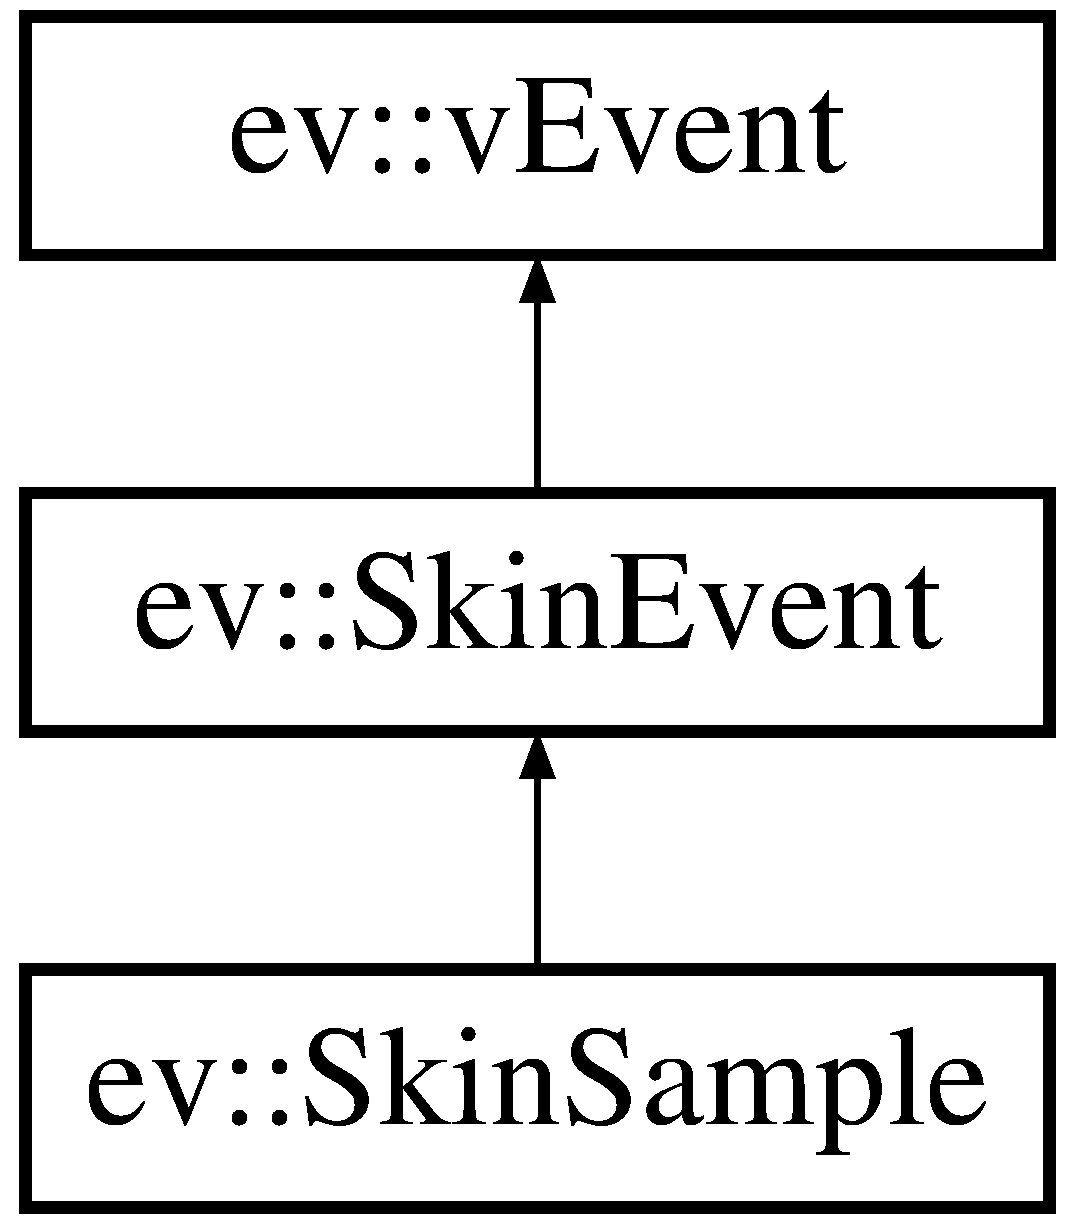
\includegraphics[height=3.000000cm]{classev_1_1SkinSample}
\end{center}
\end{figure}
\subsection*{Public Member Functions}
\begin{DoxyCompactItemize}
\item 
\mbox{\Hypertarget{classev_1_1SkinSample_a86431fb3cf157ed4bdf4945800d6a322}\label{classev_1_1SkinSample_a86431fb3cf157ed4bdf4945800d6a322}} 
{\bfseries Skin\+Sample} (const \hyperlink{classev_1_1vEvent}{v\+Event} \&v)
\item 
\mbox{\Hypertarget{classev_1_1SkinSample_af786fa6b5a90decbeea3e07463de1fc6}\label{classev_1_1SkinSample_af786fa6b5a90decbeea3e07463de1fc6}} 
{\bfseries Skin\+Sample} (const \hyperlink{classev_1_1SkinSample}{Skin\+Sample} \&v)
\item 
\mbox{\Hypertarget{classev_1_1SkinSample_ab3a5efb43e33bd9d850d453528f14a2d}\label{classev_1_1SkinSample_ab3a5efb43e33bd9d850d453528f14a2d}} 
virtual event {\bfseries clone} ()
\item 
\mbox{\Hypertarget{classev_1_1SkinSample_a92eceaf22956154e9542666fddca3033}\label{classev_1_1SkinSample_a92eceaf22956154e9542666fddca3033}} 
virtual void {\bfseries encode} (yarp\+::os\+::\+Bottle \&b) const
\item 
\mbox{\Hypertarget{classev_1_1SkinSample_a289c3ea0ff427774ca9b8130c4baa582}\label{classev_1_1SkinSample_a289c3ea0ff427774ca9b8130c4baa582}} 
virtual void {\bfseries encode} (std\+::vector$<$ int32\+\_\+t $>$ \&b, unsigned int \&pos) const
\item 
\mbox{\Hypertarget{classev_1_1SkinSample_aa20e0f7f80901929b4e62d35ea31b154}\label{classev_1_1SkinSample_aa20e0f7f80901929b4e62d35ea31b154}} 
virtual bool {\bfseries decode} (const yarp\+::os\+::\+Bottle \&packet, size\+\_\+t \&pos)
\item 
\mbox{\Hypertarget{classev_1_1SkinSample_a68e23ad4982187ceb71c7da352a5d176}\label{classev_1_1SkinSample_a68e23ad4982187ceb71c7da352a5d176}} 
virtual void {\bfseries decode} (const int32\+\_\+t $\ast$\&data)
\item 
\mbox{\Hypertarget{classev_1_1SkinSample_a7217f41079feb258f2d7fe7b78343d0e}\label{classev_1_1SkinSample_a7217f41079feb258f2d7fe7b78343d0e}} 
virtual yarp\+::os\+::\+Property {\bfseries get\+Content} () const
\item 
\mbox{\Hypertarget{classev_1_1SkinSample_a155fa0df968551153daf45139a38c5a5}\label{classev_1_1SkinSample_a155fa0df968551153daf45139a38c5a5}} 
virtual std\+::string {\bfseries get\+Type} () const
\end{DoxyCompactItemize}
\subsection*{Public Attributes}
\begin{DoxyCompactItemize}
\item 
\mbox{\Hypertarget{classev_1_1SkinSample_ac1f3f8035d23ba4450b1e852f3422825}\label{classev_1_1SkinSample_ac1f3f8035d23ba4450b1e852f3422825}} 
unsigned int {\bfseries \+\_\+ts}\+:31
\item 
\mbox{\Hypertarget{classev_1_1SkinSample_a23534f3787cad7c9d1c8c2ba8bf5bbf4}\label{classev_1_1SkinSample_a23534f3787cad7c9d1c8c2ba8bf5bbf4}} 
unsigned int {\bfseries value}\+:16
\end{DoxyCompactItemize}
\subsection*{Static Public Attributes}
\begin{DoxyCompactItemize}
\item 
\mbox{\Hypertarget{classev_1_1SkinSample_a40d0036de84cc8071b85157fccb2db54}\label{classev_1_1SkinSample_a40d0036de84cc8071b85157fccb2db54}} 
static const std\+::string {\bfseries tag} = \char`\"{}S\+KS\char`\"{}
\end{DoxyCompactItemize}


\subsection{Detailed Description}
an event with a taxel location, body-\/part and polarity 

The documentation for this class was generated from the following files\+:\begin{DoxyCompactItemize}
\item 
/mnt/d/projects/event-\/driven/lib/include/event-\/driven/v\+Codec.\+h\item 
/mnt/d/projects/event-\/driven/lib/src/codecs/codec\+\_\+\+Skin\+Sample.\+cpp\end{DoxyCompactItemize}

\hypertarget{classev_1_1skinsampleDraw}{}\section{ev\+:\+:skinsample\+Draw Class Reference}
\label{classev_1_1skinsampleDraw}\index{ev\+::skinsample\+Draw@{ev\+::skinsample\+Draw}}
Inheritance diagram for ev\+:\+:skinsample\+Draw\+:\begin{figure}[H]
\begin{center}
\leavevmode
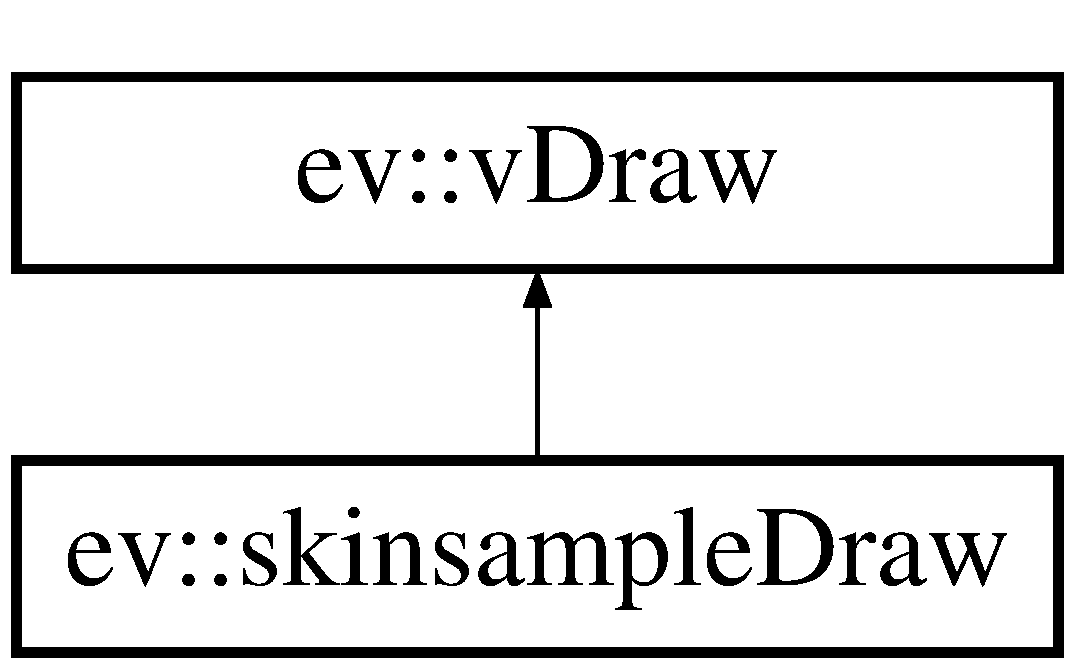
\includegraphics[height=2.000000cm]{classev_1_1skinsampleDraw}
\end{center}
\end{figure}
\subsection*{Public Member Functions}
\begin{DoxyCompactItemize}
\item 
\mbox{\Hypertarget{classev_1_1skinsampleDraw_a1ea80b10daa9076585204aa3e30613c1}\label{classev_1_1skinsampleDraw_a1ea80b10daa9076585204aa3e30613c1}} 
void {\bfseries initialise} ()
\item 
\mbox{\Hypertarget{classev_1_1skinsampleDraw_a0cf801e4cf816bb9c6ab4a2eb16dfe44}\label{classev_1_1skinsampleDraw_a0cf801e4cf816bb9c6ab4a2eb16dfe44}} 
virtual void {\bfseries reset\+Image} (cv\+::\+Mat \&image)
\item 
virtual void \hyperlink{classev_1_1skinsampleDraw_a1c2492038e7fe94fe88d2286ac18f2c6}{draw} (cv\+::\+Mat \&image, const ev\+::v\+Queue \&e\+Set, int v\+Time)
\begin{DoxyCompactList}\small\item\em draw takes an image and overlays the new visualisation textures \end{DoxyCompactList}\item 
virtual std\+::string \hyperlink{classev_1_1skinsampleDraw_a32064d959f2c127d25a9fa6773384850}{get\+Draw\+Type} ()
\begin{DoxyCompactList}\small\item\em get\+Tag returns the unique code for this drawing method. The arguments given on the command line must match this code exactly \end{DoxyCompactList}\item 
\mbox{\Hypertarget{classev_1_1skinsampleDraw_a7b7075fd4bf79d11456df8dc9b5c42a5}\label{classev_1_1skinsampleDraw_a7b7075fd4bf79d11456df8dc9b5c42a5}} 
virtual std\+::string {\bfseries get\+Event\+Type} ()
\end{DoxyCompactItemize}
\subsection*{Static Public Attributes}
\begin{DoxyCompactItemize}
\item 
\mbox{\Hypertarget{classev_1_1skinsampleDraw_a1519aa476ab6326a0c509b6100c2df5c}\label{classev_1_1skinsampleDraw_a1519aa476ab6326a0c509b6100c2df5c}} 
static const std\+::string {\bfseries drawtype} = \char`\"{}S\+A\+M\+P\+LE\char`\"{}
\end{DoxyCompactItemize}
\subsection*{Additional Inherited Members}


\subsection{Member Function Documentation}
\mbox{\Hypertarget{classev_1_1skinsampleDraw_a1c2492038e7fe94fe88d2286ac18f2c6}\label{classev_1_1skinsampleDraw_a1c2492038e7fe94fe88d2286ac18f2c6}} 
\index{ev\+::skinsample\+Draw@{ev\+::skinsample\+Draw}!draw@{draw}}
\index{draw@{draw}!ev\+::skinsample\+Draw@{ev\+::skinsample\+Draw}}
\subsubsection{\texorpdfstring{draw()}{draw()}}
{\footnotesize\ttfamily void ev\+::skinsample\+Draw\+::draw (\begin{DoxyParamCaption}\item[{cv\+::\+Mat \&}]{canvas,  }\item[{const ev\+::v\+Queue \&}]{e\+Set,  }\item[{int}]{v\+Time }\end{DoxyParamCaption})\hspace{0.3cm}{\ttfamily [virtual]}}



draw takes an image and overlays the new visualisation textures 


\begin{DoxyParams}{Parameters}
{\em canvas} & is the image which may or may not yet exist \\
\hline
{\em e\+Set} & is the set of events which could possibly be drawn \\
\hline
\end{DoxyParams}


Implements \hyperlink{classev_1_1vDraw_af1eee5dcdf3b4cfee6a3024e5cd706f8}{ev\+::v\+Draw}.

\mbox{\Hypertarget{classev_1_1skinsampleDraw_a32064d959f2c127d25a9fa6773384850}\label{classev_1_1skinsampleDraw_a32064d959f2c127d25a9fa6773384850}} 
\index{ev\+::skinsample\+Draw@{ev\+::skinsample\+Draw}!get\+Draw\+Type@{get\+Draw\+Type}}
\index{get\+Draw\+Type@{get\+Draw\+Type}!ev\+::skinsample\+Draw@{ev\+::skinsample\+Draw}}
\subsubsection{\texorpdfstring{get\+Draw\+Type()}{getDrawType()}}
{\footnotesize\ttfamily std\+::string ev\+::skinsample\+Draw\+::get\+Draw\+Type (\begin{DoxyParamCaption}{ }\end{DoxyParamCaption})\hspace{0.3cm}{\ttfamily [virtual]}}



get\+Tag returns the unique code for this drawing method. The arguments given on the command line must match this code exactly 

\begin{DoxyReturn}{Returns}
the tag code 
\end{DoxyReturn}


Implements \hyperlink{classev_1_1vDraw_ac01381befeffef2b930cbceb28b18a28}{ev\+::v\+Draw}.



The documentation for this class was generated from the following files\+:\begin{DoxyCompactItemize}
\item 
/mnt/d/projects/event-\/driven/lib/include/event-\/driven/v\+Draw\+Skin.\+h\item 
/mnt/d/projects/event-\/driven/lib/src/v\+Draw\+\_\+skin.\+cpp\end{DoxyCompactItemize}

\hypertarget{classev_1_1surfaceThread}{}\section{ev\+:\+:surface\+Thread Class Reference}
\label{classev_1_1surfaceThread}\index{ev\+::surface\+Thread@{ev\+::surface\+Thread}}


asynchronously read events and push them in a \hyperlink{classev_1_1vSurface}{v\+Surface}  




{\ttfamily \#include $<$v\+Surface\+Handler\+Th.\+h$>$}

Inheritance diagram for ev\+:\+:surface\+Thread\+:\begin{figure}[H]
\begin{center}
\leavevmode
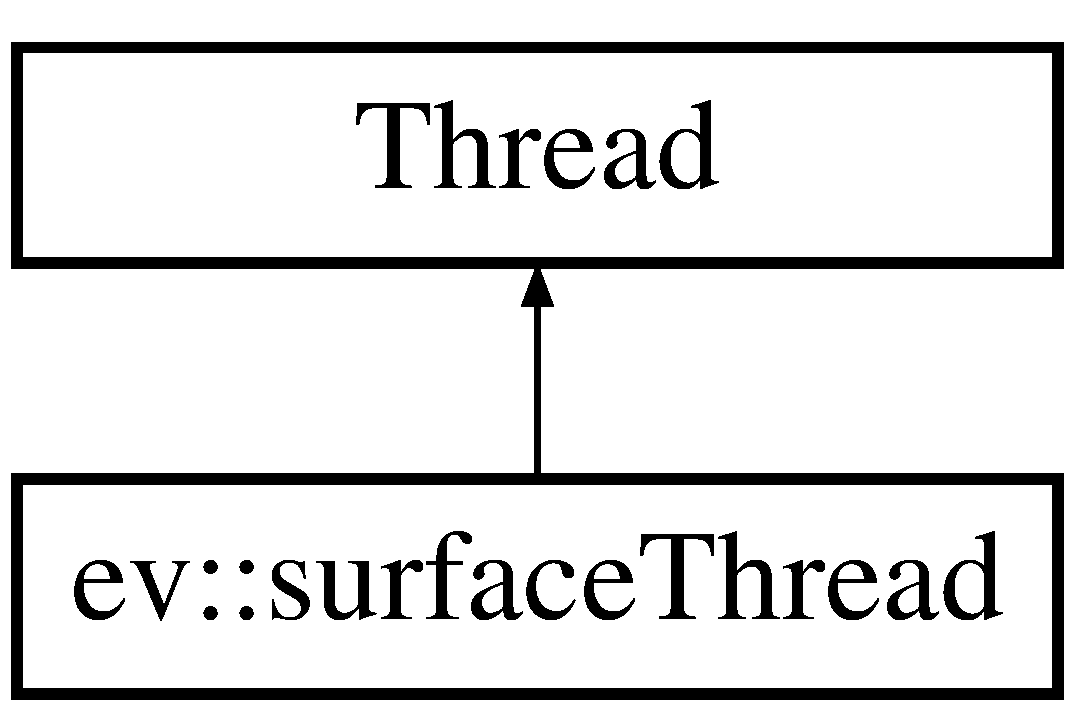
\includegraphics[height=2.000000cm]{classev_1_1surfaceThread}
\end{center}
\end{figure}
\subsection*{Public Member Functions}
\begin{DoxyCompactItemize}
\item 
\mbox{\Hypertarget{classev_1_1surfaceThread_a17d8e5af5b6617d91631fe3565e7ec21}\label{classev_1_1surfaceThread_a17d8e5af5b6617d91631fe3565e7ec21}} 
void {\bfseries configure} (int height, int width)
\item 
\mbox{\Hypertarget{classev_1_1surfaceThread_a8fbb7a7f67aeb8766ee1d222550306c9}\label{classev_1_1surfaceThread_a8fbb7a7f67aeb8766ee1d222550306c9}} 
bool {\bfseries open} (std\+::string portname)
\item 
\mbox{\Hypertarget{classev_1_1surfaceThread_a65d324c3c3d8f699412f4fa1eb5aff62}\label{classev_1_1surfaceThread_a65d324c3c3d8f699412f4fa1eb5aff62}} 
void {\bfseries on\+Stop} ()
\item 
\mbox{\Hypertarget{classev_1_1surfaceThread_a04b53ae45896e77a84db501ddfc956cf}\label{classev_1_1surfaceThread_a04b53ae45896e77a84db501ddfc956cf}} 
void {\bfseries run} ()
\item 
\mbox{\Hypertarget{classev_1_1surfaceThread_a04b8a2e62c4910346bdfc2ae9c82371b}\label{classev_1_1surfaceThread_a04b8a2e62c4910346bdfc2ae9c82371b}} 
yarp\+::os\+::\+Stamp {\bfseries query\+R\+OI} (ev\+::v\+Queue \&fillq, int c, unsigned int t, int x, int y, int r)
\item 
\mbox{\Hypertarget{classev_1_1surfaceThread_ad552b309bca76006c5e8adc07fdcbb6a}\label{classev_1_1surfaceThread_ad552b309bca76006c5e8adc07fdcbb6a}} 
yarp\+::os\+::\+Stamp {\bfseries query\+Window} (ev\+::v\+Queue \&fillq, int c, unsigned int t)
\item 
\mbox{\Hypertarget{classev_1_1surfaceThread_a763bb2d669fdc772316f074fd43c82d8}\label{classev_1_1surfaceThread_a763bb2d669fdc772316f074fd43c82d8}} 
unsigned int {\bfseries query\+V\+Time} ()
\end{DoxyCompactItemize}


\subsection{Detailed Description}
asynchronously read events and push them in a \hyperlink{classev_1_1vSurface}{v\+Surface} 

The documentation for this class was generated from the following file\+:\begin{DoxyCompactItemize}
\item 
/mnt/d/projects/event-\/driven/lib/include/event-\/driven/v\+Surface\+Handler\+Th.\+h\end{DoxyCompactItemize}

\hypertarget{classev_1_1syncvstreams}{}\section{ev\+:\+:syncvstreams Class Reference}
\label{classev_1_1syncvstreams}\index{ev\+::syncvstreams@{ev\+::syncvstreams}}


automatically accept multiple event types from different ports (e.\+g. as in the v\+Framer)  




{\ttfamily \#include $<$v\+Surface\+Handler\+Th.\+h$>$}

\subsection*{Public Member Functions}
\begin{DoxyCompactItemize}
\item 
\mbox{\Hypertarget{classev_1_1syncvstreams_acc652540f64e92a0528e25932ff51d8f}\label{classev_1_1syncvstreams_acc652540f64e92a0528e25932ff51d8f}} 
bool {\bfseries open} (std\+::string module\+Name, std\+::string event\+Type)
\item 
\mbox{\Hypertarget{classev_1_1syncvstreams_a347bea90f23cf334667bb3e4b7bcf7a0}\label{classev_1_1syncvstreams_a347bea90f23cf334667bb3e4b7bcf7a0}} 
v\+Queue {\bfseries query\+Window} (std\+::string v\+Type, int channel)
\item 
\mbox{\Hypertarget{classev_1_1syncvstreams_a04f3e59f95d0749a6ceff9d7e426fb5d}\label{classev_1_1syncvstreams_a04f3e59f95d0749a6ceff9d7e426fb5d}} 
void {\bfseries update\+Stamps} ()
\item 
\mbox{\Hypertarget{classev_1_1syncvstreams_ae4bdb73e97024c7399d8a105bdc8425a}\label{classev_1_1syncvstreams_ae4bdb73e97024c7399d8a105bdc8425a}} 
void {\bfseries close} ()
\item 
\mbox{\Hypertarget{classev_1_1syncvstreams_a61e65f054ee803198d3e642df2bc1024}\label{classev_1_1syncvstreams_a61e65f054ee803198d3e642df2bc1024}} 
yarp\+::os\+::\+Stamp {\bfseries getystamp} ()
\item 
\mbox{\Hypertarget{classev_1_1syncvstreams_a8846f86bb2794a7b6117c4f9d9c9fa65}\label{classev_1_1syncvstreams_a8846f86bb2794a7b6117c4f9d9c9fa65}} 
int {\bfseries getvstamp} ()
\item 
\mbox{\Hypertarget{classev_1_1syncvstreams_a83d0eb380a6a8eda16f35b45a7773da6}\label{classev_1_1syncvstreams_a83d0eb380a6a8eda16f35b45a7773da6}} 
void {\bfseries set\+Strict\+Update\+Period} (int period)
\item 
\mbox{\Hypertarget{classev_1_1syncvstreams_adff155da0d9cf739725127c446b1e575}\label{classev_1_1syncvstreams_adff155da0d9cf739725127c446b1e575}} 
bool {\bfseries has\+Updated} ()
\item 
\mbox{\Hypertarget{classev_1_1syncvstreams_a481bbbc4b4a0b4d7721e630da92de71c}\label{classev_1_1syncvstreams_a481bbbc4b4a0b4d7721e630da92de71c}} 
unsigned int {\bfseries query\+Max\+Unproced} ()
\item 
\mbox{\Hypertarget{classev_1_1syncvstreams_a40bb750373f2b6d406e57bbd70bc40b1}\label{classev_1_1syncvstreams_a40bb750373f2b6d406e57bbd70bc40b1}} 
std\+::string {\bfseries delay\+Stats} ()
\end{DoxyCompactItemize}


\subsection{Detailed Description}
automatically accept multiple event types from different ports (e.\+g. as in the v\+Framer) 

The documentation for this class was generated from the following file\+:\begin{DoxyCompactItemize}
\item 
/mnt/d/projects/event-\/driven/lib/include/event-\/driven/v\+Surface\+Handler\+Th.\+h\end{DoxyCompactItemize}

\hypertarget{classev_1_1taxeleventDraw}{}\section{ev\+:\+:taxelevent\+Draw Class Reference}
\label{classev_1_1taxeleventDraw}\index{ev\+::taxelevent\+Draw@{ev\+::taxelevent\+Draw}}
Inheritance diagram for ev\+:\+:taxelevent\+Draw\+:\begin{figure}[H]
\begin{center}
\leavevmode
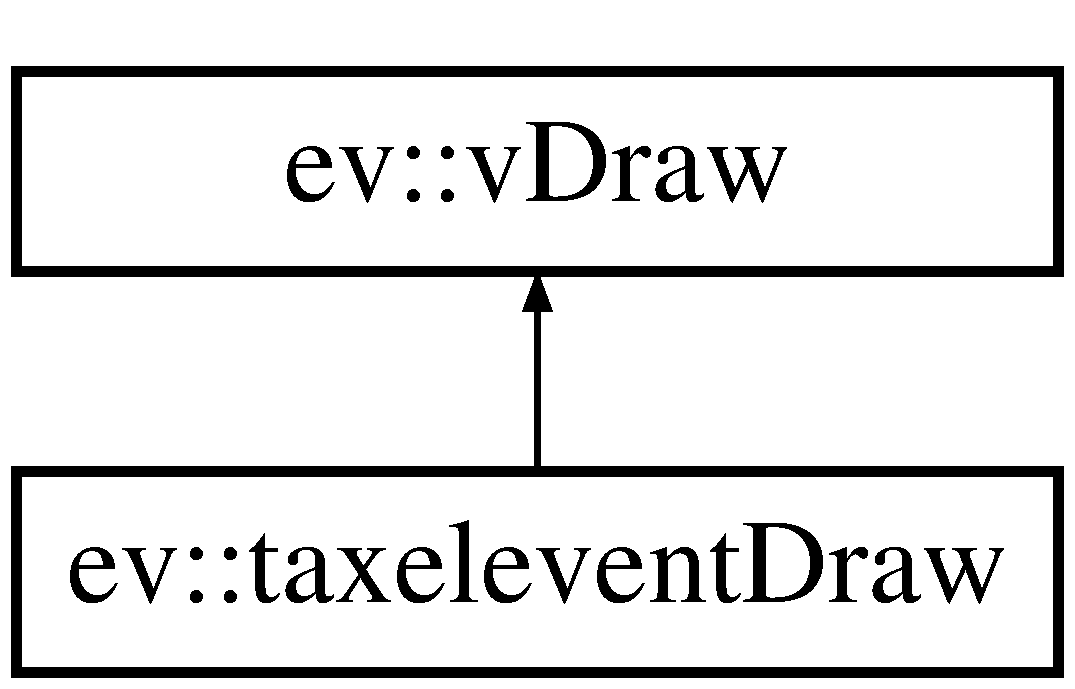
\includegraphics[height=2.000000cm]{classev_1_1taxeleventDraw}
\end{center}
\end{figure}
\subsection*{Public Member Functions}
\begin{DoxyCompactItemize}
\item 
\mbox{\Hypertarget{classev_1_1taxeleventDraw_a0d36f9cfb5b25f484a673a5b4e87212d}\label{classev_1_1taxeleventDraw_a0d36f9cfb5b25f484a673a5b4e87212d}} 
virtual void {\bfseries reset\+Image} (cv\+::\+Mat \&image)
\item 
\mbox{\Hypertarget{classev_1_1taxeleventDraw_a1f3b8b62fcb02639932f776b4bb99bd1}\label{classev_1_1taxeleventDraw_a1f3b8b62fcb02639932f776b4bb99bd1}} 
void {\bfseries initialise} ()
\item 
virtual void \hyperlink{classev_1_1taxeleventDraw_ad2ff0348ee1b362e3c50508ffefdf9d1}{draw} (cv\+::\+Mat \&image, const ev\+::v\+Queue \&e\+Set, int v\+Time)
\begin{DoxyCompactList}\small\item\em draw takes an image and overlays the new visualisation textures \end{DoxyCompactList}\item 
virtual std\+::string \hyperlink{classev_1_1taxeleventDraw_a474b409ea48a97749caaf172f5fd467a}{get\+Draw\+Type} ()
\begin{DoxyCompactList}\small\item\em get\+Tag returns the unique code for this drawing method. The arguments given on the command line must match this code exactly \end{DoxyCompactList}\item 
\mbox{\Hypertarget{classev_1_1taxeleventDraw_ae3f6ee8378f0f99c653b6ed648fdf88c}\label{classev_1_1taxeleventDraw_ae3f6ee8378f0f99c653b6ed648fdf88c}} 
virtual std\+::string {\bfseries get\+Event\+Type} ()
\end{DoxyCompactItemize}
\subsection*{Static Public Attributes}
\begin{DoxyCompactItemize}
\item 
\mbox{\Hypertarget{classev_1_1taxeleventDraw_af7df65142d28c9a698b33622ded9169c}\label{classev_1_1taxeleventDraw_af7df65142d28c9a698b33622ded9169c}} 
static const std\+::string {\bfseries drawtype} = \char`\"{}T\+A\+X\+E\+L\+\_\+\+E\+V\+E\+NT\char`\"{}
\end{DoxyCompactItemize}
\subsection*{Additional Inherited Members}


\subsection{Member Function Documentation}
\mbox{\Hypertarget{classev_1_1taxeleventDraw_ad2ff0348ee1b362e3c50508ffefdf9d1}\label{classev_1_1taxeleventDraw_ad2ff0348ee1b362e3c50508ffefdf9d1}} 
\index{ev\+::taxelevent\+Draw@{ev\+::taxelevent\+Draw}!draw@{draw}}
\index{draw@{draw}!ev\+::taxelevent\+Draw@{ev\+::taxelevent\+Draw}}
\subsubsection{\texorpdfstring{draw()}{draw()}}
{\footnotesize\ttfamily void ev\+::taxelevent\+Draw\+::draw (\begin{DoxyParamCaption}\item[{cv\+::\+Mat \&}]{canvas,  }\item[{const ev\+::v\+Queue \&}]{e\+Set,  }\item[{int}]{v\+Time }\end{DoxyParamCaption})\hspace{0.3cm}{\ttfamily [virtual]}}



draw takes an image and overlays the new visualisation textures 


\begin{DoxyParams}{Parameters}
{\em canvas} & is the image which may or may not yet exist \\
\hline
{\em e\+Set} & is the set of events which could possibly be drawn \\
\hline
\end{DoxyParams}


Implements \hyperlink{classev_1_1vDraw_af1eee5dcdf3b4cfee6a3024e5cd706f8}{ev\+::v\+Draw}.

\mbox{\Hypertarget{classev_1_1taxeleventDraw_a474b409ea48a97749caaf172f5fd467a}\label{classev_1_1taxeleventDraw_a474b409ea48a97749caaf172f5fd467a}} 
\index{ev\+::taxelevent\+Draw@{ev\+::taxelevent\+Draw}!get\+Draw\+Type@{get\+Draw\+Type}}
\index{get\+Draw\+Type@{get\+Draw\+Type}!ev\+::taxelevent\+Draw@{ev\+::taxelevent\+Draw}}
\subsubsection{\texorpdfstring{get\+Draw\+Type()}{getDrawType()}}
{\footnotesize\ttfamily std\+::string ev\+::taxelevent\+Draw\+::get\+Draw\+Type (\begin{DoxyParamCaption}{ }\end{DoxyParamCaption})\hspace{0.3cm}{\ttfamily [virtual]}}



get\+Tag returns the unique code for this drawing method. The arguments given on the command line must match this code exactly 

\begin{DoxyReturn}{Returns}
the tag code 
\end{DoxyReturn}


Implements \hyperlink{classev_1_1vDraw_ac01381befeffef2b930cbceb28b18a28}{ev\+::v\+Draw}.



The documentation for this class was generated from the following files\+:\begin{DoxyCompactItemize}
\item 
/mnt/d/projects/event-\/driven/lib/include/event-\/driven/v\+Draw\+Skin.\+h\item 
/mnt/d/projects/event-\/driven/lib/src/v\+Draw\+\_\+skin.\+cpp\end{DoxyCompactItemize}

\hypertarget{classev_1_1taxelsampleDraw}{}\section{ev\+:\+:taxelsample\+Draw Class Reference}
\label{classev_1_1taxelsampleDraw}\index{ev\+::taxelsample\+Draw@{ev\+::taxelsample\+Draw}}
Inheritance diagram for ev\+:\+:taxelsample\+Draw\+:\begin{figure}[H]
\begin{center}
\leavevmode
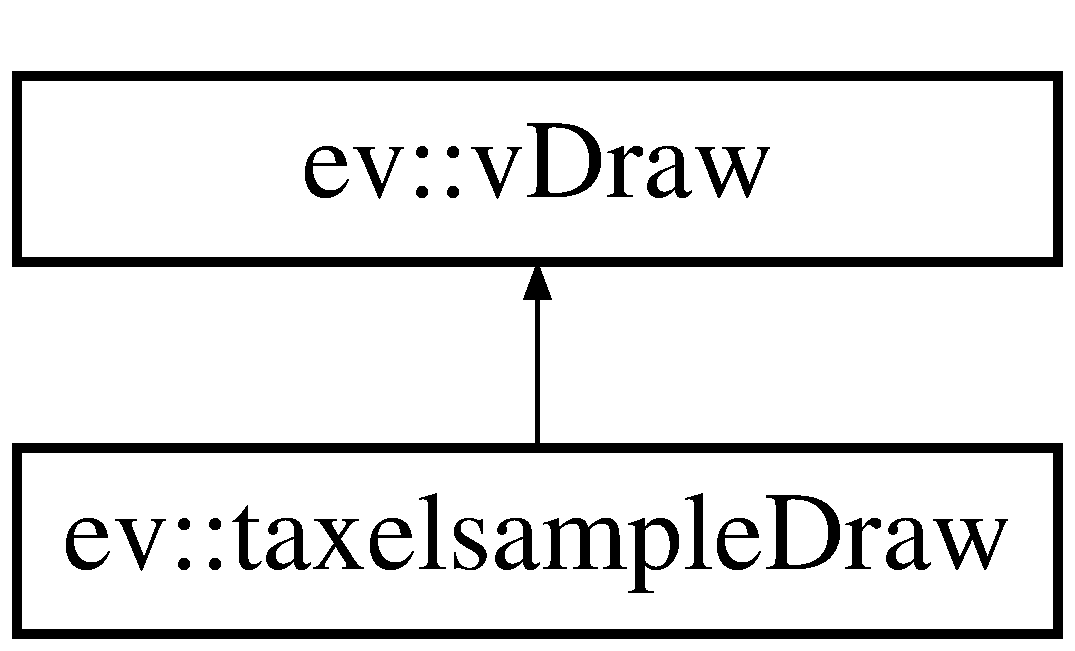
\includegraphics[height=2.000000cm]{classev_1_1taxelsampleDraw}
\end{center}
\end{figure}
\subsection*{Public Member Functions}
\begin{DoxyCompactItemize}
\item 
\mbox{\Hypertarget{classev_1_1taxelsampleDraw_ae3b414d9cc7894b504683f0af8059d89}\label{classev_1_1taxelsampleDraw_ae3b414d9cc7894b504683f0af8059d89}} 
void {\bfseries reset\+Image} (cv\+::\+Mat \&image)
\item 
\mbox{\Hypertarget{classev_1_1taxelsampleDraw_a9d69dcd342df4005f86966f18b8b31c4}\label{classev_1_1taxelsampleDraw_a9d69dcd342df4005f86966f18b8b31c4}} 
void {\bfseries initialise} ()
\item 
virtual void \hyperlink{classev_1_1taxelsampleDraw_a43e40e8cfc4ed342f8d616eb9ddecf0a}{draw} (cv\+::\+Mat \&image, const ev\+::v\+Queue \&e\+Set, int v\+Time)
\begin{DoxyCompactList}\small\item\em draw takes an image and overlays the new visualisation textures \end{DoxyCompactList}\item 
virtual std\+::string \hyperlink{classev_1_1taxelsampleDraw_a7bf19e7de1e4851b5567308e95334942}{get\+Draw\+Type} ()
\begin{DoxyCompactList}\small\item\em get\+Tag returns the unique code for this drawing method. The arguments given on the command line must match this code exactly \end{DoxyCompactList}\item 
\mbox{\Hypertarget{classev_1_1taxelsampleDraw_ac02cc2de0555b249d6a0df31f7954140}\label{classev_1_1taxelsampleDraw_ac02cc2de0555b249d6a0df31f7954140}} 
virtual std\+::string {\bfseries get\+Event\+Type} ()
\end{DoxyCompactItemize}
\subsection*{Static Public Attributes}
\begin{DoxyCompactItemize}
\item 
\mbox{\Hypertarget{classev_1_1taxelsampleDraw_a461de248c8eee82c8f2a88a24a919992}\label{classev_1_1taxelsampleDraw_a461de248c8eee82c8f2a88a24a919992}} 
static const std\+::string {\bfseries drawtype} = \char`\"{}T\+A\+X\+E\+L\+\_\+\+S\+A\+M\+P\+LE\char`\"{}
\end{DoxyCompactItemize}
\subsection*{Additional Inherited Members}


\subsection{Member Function Documentation}
\mbox{\Hypertarget{classev_1_1taxelsampleDraw_a43e40e8cfc4ed342f8d616eb9ddecf0a}\label{classev_1_1taxelsampleDraw_a43e40e8cfc4ed342f8d616eb9ddecf0a}} 
\index{ev\+::taxelsample\+Draw@{ev\+::taxelsample\+Draw}!draw@{draw}}
\index{draw@{draw}!ev\+::taxelsample\+Draw@{ev\+::taxelsample\+Draw}}
\subsubsection{\texorpdfstring{draw()}{draw()}}
{\footnotesize\ttfamily void ev\+::taxelsample\+Draw\+::draw (\begin{DoxyParamCaption}\item[{cv\+::\+Mat \&}]{canvas,  }\item[{const ev\+::v\+Queue \&}]{e\+Set,  }\item[{int}]{v\+Time }\end{DoxyParamCaption})\hspace{0.3cm}{\ttfamily [virtual]}}



draw takes an image and overlays the new visualisation textures 


\begin{DoxyParams}{Parameters}
{\em canvas} & is the image which may or may not yet exist \\
\hline
{\em e\+Set} & is the set of events which could possibly be drawn \\
\hline
\end{DoxyParams}


Implements \hyperlink{classev_1_1vDraw_af1eee5dcdf3b4cfee6a3024e5cd706f8}{ev\+::v\+Draw}.

\mbox{\Hypertarget{classev_1_1taxelsampleDraw_a7bf19e7de1e4851b5567308e95334942}\label{classev_1_1taxelsampleDraw_a7bf19e7de1e4851b5567308e95334942}} 
\index{ev\+::taxelsample\+Draw@{ev\+::taxelsample\+Draw}!get\+Draw\+Type@{get\+Draw\+Type}}
\index{get\+Draw\+Type@{get\+Draw\+Type}!ev\+::taxelsample\+Draw@{ev\+::taxelsample\+Draw}}
\subsubsection{\texorpdfstring{get\+Draw\+Type()}{getDrawType()}}
{\footnotesize\ttfamily std\+::string ev\+::taxelsample\+Draw\+::get\+Draw\+Type (\begin{DoxyParamCaption}{ }\end{DoxyParamCaption})\hspace{0.3cm}{\ttfamily [virtual]}}



get\+Tag returns the unique code for this drawing method. The arguments given on the command line must match this code exactly 

\begin{DoxyReturn}{Returns}
the tag code 
\end{DoxyReturn}


Implements \hyperlink{classev_1_1vDraw_ac01381befeffef2b930cbceb28b18a28}{ev\+::v\+Draw}.



The documentation for this class was generated from the following files\+:\begin{DoxyCompactItemize}
\item 
/mnt/d/projects/event-\/driven/lib/include/event-\/driven/v\+Draw\+Skin.\+h\item 
/mnt/d/projects/event-\/driven/lib/src/v\+Draw\+\_\+skin.\+cpp\end{DoxyCompactItemize}

\hypertarget{classev_1_1temporalSurface}{}\section{ev\+:\+:temporal\+Surface Class Reference}
\label{classev_1_1temporalSurface}\index{ev\+::temporal\+Surface@{ev\+::temporal\+Surface}}


a spatio-\/temporal surface storing events for a limited time  




{\ttfamily \#include $<$v\+Window\+\_\+adv.\+h$>$}

Inheritance diagram for ev\+:\+:temporal\+Surface\+:\begin{figure}[H]
\begin{center}
\leavevmode
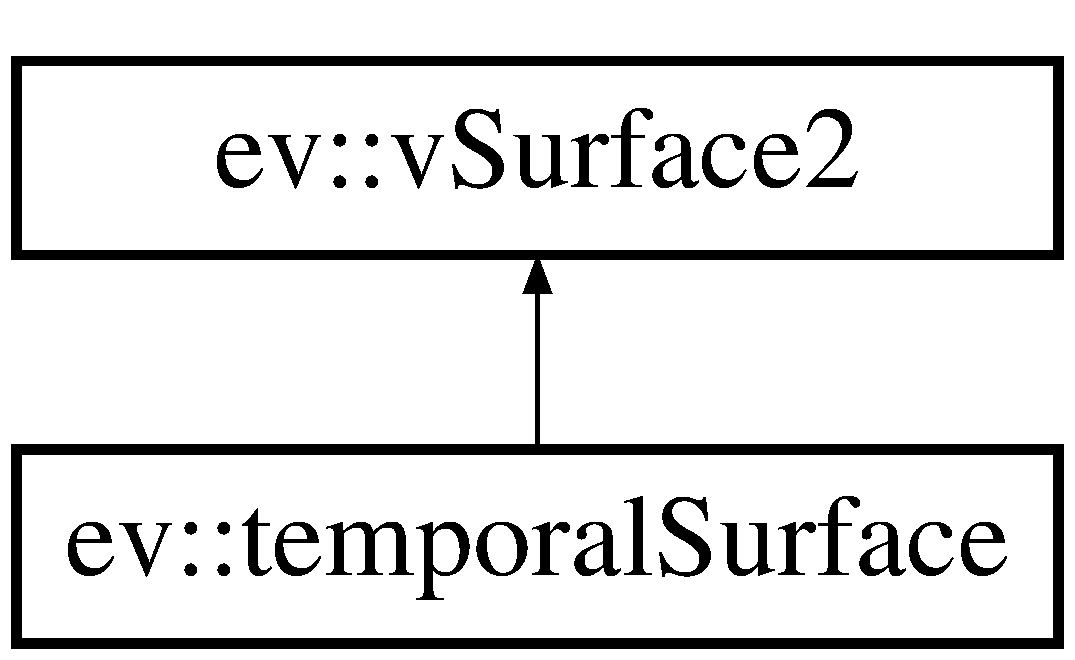
\includegraphics[height=2.000000cm]{classev_1_1temporalSurface}
\end{center}
\end{figure}
\subsection*{Public Member Functions}
\begin{DoxyCompactItemize}
\item 
\mbox{\Hypertarget{classev_1_1temporalSurface_a5fe8e1a5c4011ab466a42855e286d3c8}\label{classev_1_1temporalSurface_a5fe8e1a5c4011ab466a42855e286d3c8}} 
{\bfseries temporal\+Surface} (int \hyperlink{classev_1_1vSurface2_a1aa8027816352a15d5b9bf1f26f48e76}{width}=128, int height=128, int duration=2.\+0 $\ast$\hyperlink{classev_1_1vtsHelper_afa2dd46ae7113668bc6ebea88ab8fa11}{vts\+Helper\+::vtsscaler})
\item 
\mbox{\Hypertarget{classev_1_1temporalSurface_a358c548e6727aa89d908e61ad948b1ca}\label{classev_1_1temporalSurface_a358c548e6727aa89d908e61ad948b1ca}} 
virtual v\+Queue {\bfseries remove\+Events} (event$<$$>$ to\+Add)
\item 
\mbox{\Hypertarget{classev_1_1temporalSurface_a78a9bb93145915a90a5105bab812bb65}\label{classev_1_1temporalSurface_a78a9bb93145915a90a5105bab812bb65}} 
virtual void {\bfseries fast\+Remove\+Events} (event$<$$>$ to\+Add)
\item 
\mbox{\Hypertarget{classev_1_1temporalSurface_a35d4b67c18393961fa833d330a040e80}\label{classev_1_1temporalSurface_a35d4b67c18393961fa833d330a040e80}} 
void {\bfseries set\+Temporal\+Size} (int duration)
\end{DoxyCompactItemize}
\subsection*{Additional Inherited Members}


\subsection{Detailed Description}
a spatio-\/temporal surface storing events for a limited time 

The documentation for this class was generated from the following files\+:\begin{DoxyCompactItemize}
\item 
/mnt/d/projects/event-\/driven/lib/include/event-\/driven/v\+Window\+\_\+adv.\+h\item 
/mnt/d/projects/event-\/driven/lib/src/v\+Window\+\_\+adv.\+cpp\end{DoxyCompactItemize}

\hypertarget{classev_1_1Triangle__10pad}{}\section{ev\+:\+:Triangle\+\_\+10pad Class Reference}
\label{classev_1_1Triangle__10pad}\index{ev\+::\+Triangle\+\_\+10pad@{ev\+::\+Triangle\+\_\+10pad}}
Inheritance diagram for ev\+:\+:Triangle\+\_\+10pad\+:\begin{figure}[H]
\begin{center}
\leavevmode
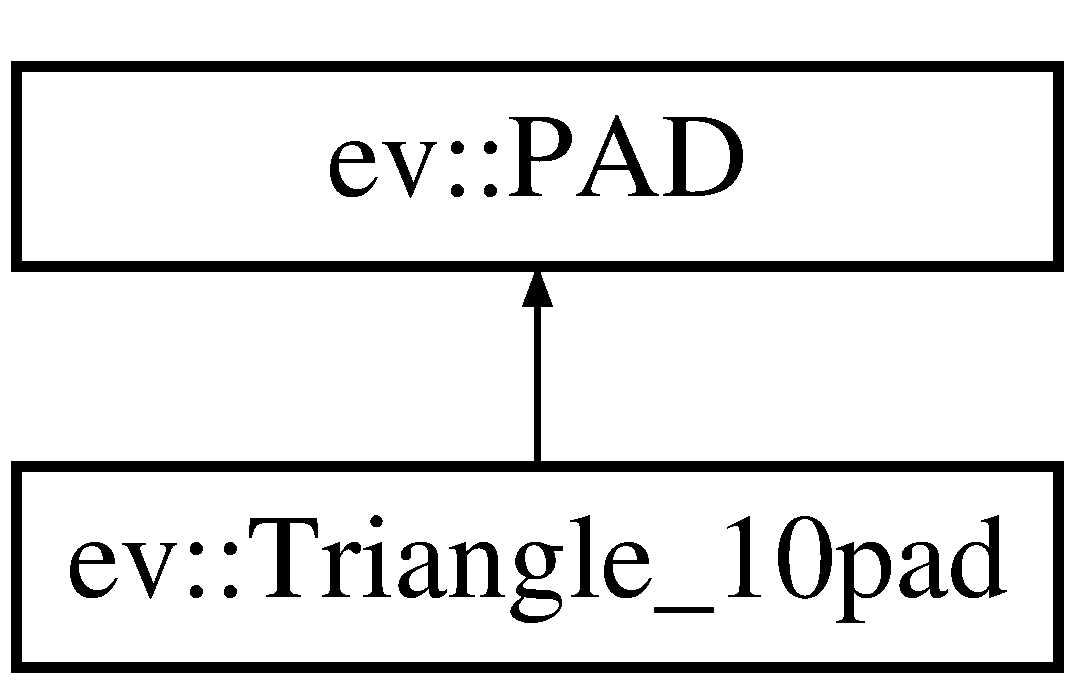
\includegraphics[height=2.000000cm]{classev_1_1Triangle__10pad}
\end{center}
\end{figure}
\subsection*{Public Member Functions}
\begin{DoxyCompactItemize}
\item 
\mbox{\Hypertarget{classev_1_1Triangle__10pad_a6b93724fa95d5c505ba997b661288d82}\label{classev_1_1Triangle__10pad_a6b93724fa95d5c505ba997b661288d82}} 
void {\bfseries init\+Representative\+Taxels} (std\+::vector$<$ int $>$ taxel\+Map)
\item 
\mbox{\Hypertarget{classev_1_1Triangle__10pad_a2da9dce32afeea094937a67d0585be9d}\label{classev_1_1Triangle__10pad_a2da9dce32afeea094937a67d0585be9d}} 
std\+::tuple$<$ double, double $>$ {\bfseries make\+Map} (int index) const
\end{DoxyCompactItemize}
\subsection*{Additional Inherited Members}


The documentation for this class was generated from the following file\+:\begin{DoxyCompactItemize}
\item 
/mnt/d/projects/event-\/driven/lib/include/event-\/driven/v\+Draw\+Skin.\+h\end{DoxyCompactItemize}

\hypertarget{classev_1_1tWinThread}{}\section{ev\+:\+:t\+Win\+Thread Class Reference}
\label{classev_1_1tWinThread}\index{ev\+::t\+Win\+Thread@{ev\+::t\+Win\+Thread}}


automatically accept events from a port and push them into a \hyperlink{classev_1_1vTempWindow}{v\+Temp\+Window}  




{\ttfamily \#include $<$v\+Surface\+Handler\+Th.\+h$>$}

Inheritance diagram for ev\+:\+:t\+Win\+Thread\+:\begin{figure}[H]
\begin{center}
\leavevmode
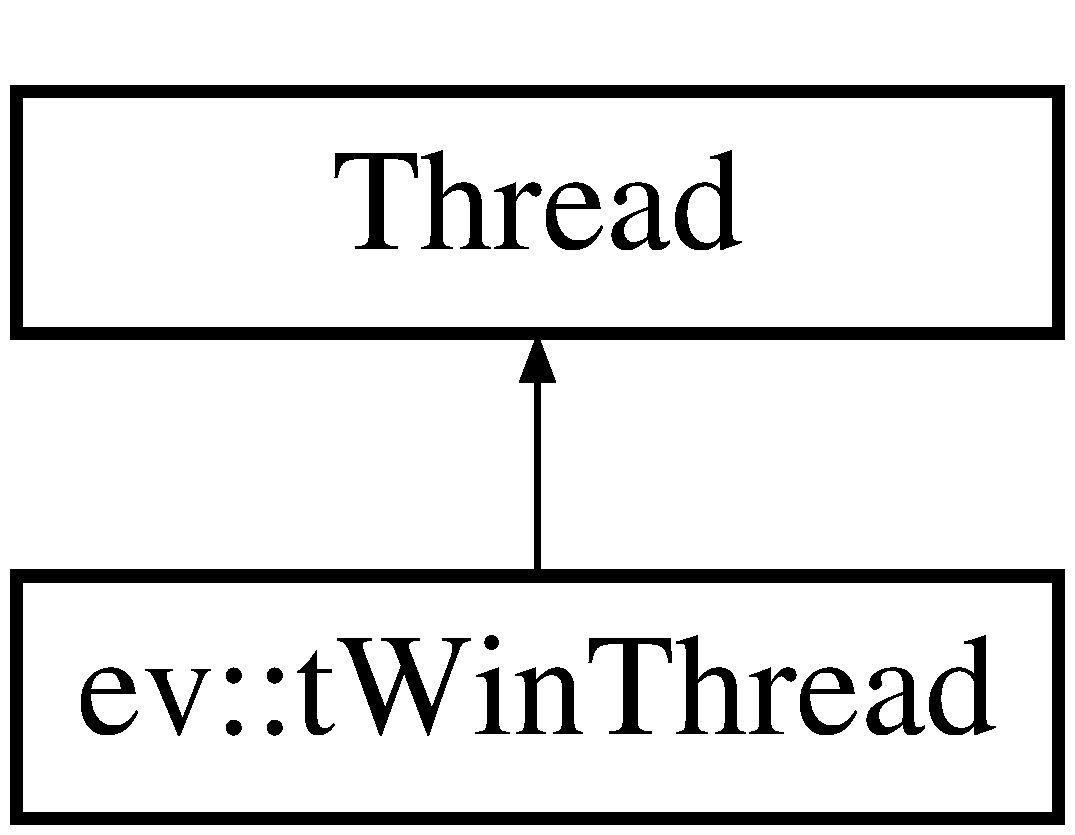
\includegraphics[height=2.000000cm]{classev_1_1tWinThread}
\end{center}
\end{figure}
\subsection*{Public Member Functions}
\begin{DoxyCompactItemize}
\item 
\mbox{\Hypertarget{classev_1_1tWinThread_a1edd593d8901ca970a51bfeb09181234}\label{classev_1_1tWinThread_a1edd593d8901ca970a51bfeb09181234}} 
bool {\bfseries open} (std\+::string portname, int period=0)
\item 
\mbox{\Hypertarget{classev_1_1tWinThread_ab12b04cd804ac7f6d2f6a199bb2078a8}\label{classev_1_1tWinThread_ab12b04cd804ac7f6d2f6a199bb2078a8}} 
void {\bfseries on\+Stop} ()
\item 
\mbox{\Hypertarget{classev_1_1tWinThread_a6992dcf7884d08d7296e4489ef264959}\label{classev_1_1tWinThread_a6992dcf7884d08d7296e4489ef264959}} 
void {\bfseries run} ()
\item 
\mbox{\Hypertarget{classev_1_1tWinThread_a6937e3d587982b4ecbc8e776c89b5ea1}\label{classev_1_1tWinThread_a6937e3d587982b4ecbc8e776c89b5ea1}} 
v\+Queue {\bfseries query\+Window} (int channel)
\item 
\mbox{\Hypertarget{classev_1_1tWinThread_a346e943bc1a1e06210deb6da26fa18f6}\label{classev_1_1tWinThread_a346e943bc1a1e06210deb6da26fa18f6}} 
void {\bfseries query\+Stamps} (yarp\+::os\+::\+Stamp \&y\+Stamp, int \&v\+Stamp)
\item 
\mbox{\Hypertarget{classev_1_1tWinThread_a4121006bf6750fb8b5d2e2844479b39f}\label{classev_1_1tWinThread_a4121006bf6750fb8b5d2e2844479b39f}} 
bool {\bfseries query\+Updated} ()
\item 
\mbox{\Hypertarget{classev_1_1tWinThread_ab3f171e6997f7e7e68abf536afa97c17}\label{classev_1_1tWinThread_ab3f171e6997f7e7e68abf536afa97c17}} 
unsigned int {\bfseries query\+Unprocd} ()
\item 
\mbox{\Hypertarget{classev_1_1tWinThread_acb5f610d1fe4e6eef43cae31c0ea0f8e}\label{classev_1_1tWinThread_acb5f610d1fe4e6eef43cae31c0ea0f8e}} 
std\+::string {\bfseries read\+Delay\+Stats} ()
\end{DoxyCompactItemize}


\subsection{Detailed Description}
automatically accept events from a port and push them into a \hyperlink{classev_1_1vTempWindow}{v\+Temp\+Window} 

The documentation for this class was generated from the following file\+:\begin{DoxyCompactItemize}
\item 
/mnt/d/projects/event-\/driven/lib/include/event-\/driven/v\+Surface\+Handler\+Th.\+h\end{DoxyCompactItemize}

\hypertarget{classev_1_1vBottle}{}\section{ev\+:\+:v\+Bottle Class Reference}
\label{classev_1_1vBottle}\index{ev\+::v\+Bottle@{ev\+::v\+Bottle}}


yarp\+::os\+::\+Bottle wrapper for sending events through the yarp system with ensuring compatibility with yarpdatadumper and yarpdataplayer  




{\ttfamily \#include $<$v\+Bottle.\+h$>$}

Inheritance diagram for ev\+:\+:v\+Bottle\+:\begin{figure}[H]
\begin{center}
\leavevmode
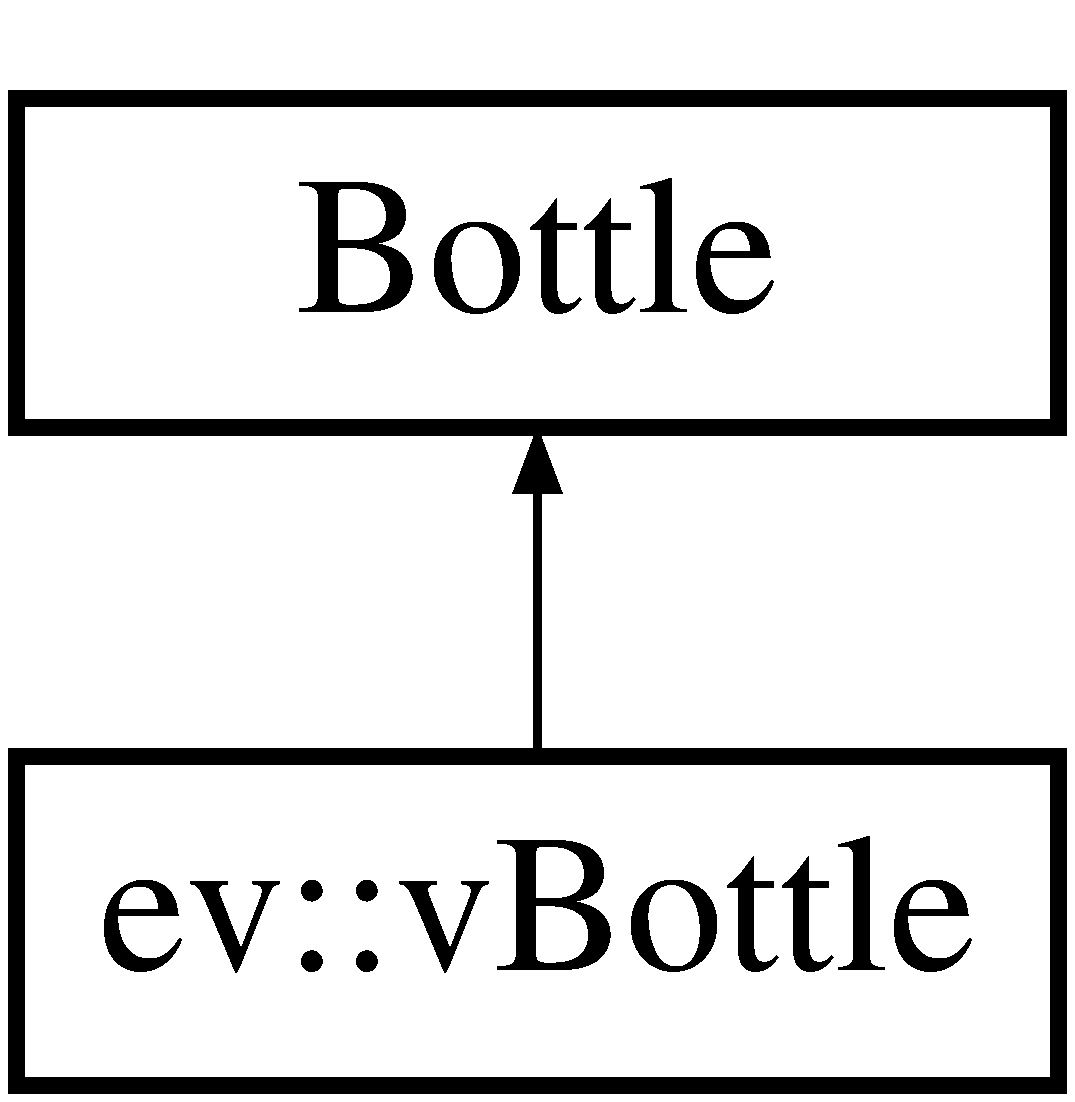
\includegraphics[height=2.000000cm]{classev_1_1vBottle}
\end{center}
\end{figure}
\subsection*{Public Member Functions}
\begin{DoxyCompactItemize}
\item 
\mbox{\Hypertarget{classev_1_1vBottle_afb002196d4fa9bd19af48be74327cb17}\label{classev_1_1vBottle_afb002196d4fa9bd19af48be74327cb17}} 
\hyperlink{classev_1_1vBottle_afb002196d4fa9bd19af48be74327cb17}{v\+Bottle} ()
\begin{DoxyCompactList}\small\item\em default constructor \end{DoxyCompactList}\item 
\mbox{\Hypertarget{classev_1_1vBottle_a5b17f0b46d9260ab255f38382b4b7268}\label{classev_1_1vBottle_a5b17f0b46d9260ab255f38382b4b7268}} 
void \hyperlink{classev_1_1vBottle_a5b17f0b46d9260ab255f38382b4b7268}{add\+Event} (event$<$$>$ e)
\begin{DoxyCompactList}\small\item\em add a single event to the \hyperlink{classev_1_1vBottle}{v\+Bottle} \end{DoxyCompactList}\item 
\mbox{\Hypertarget{classev_1_1vBottle_a0c78e6f9ef839038d71486f6a8a6294a}\label{classev_1_1vBottle_a0c78e6f9ef839038d71486f6a8a6294a}} 
void \hyperlink{classev_1_1vBottle_a0c78e6f9ef839038d71486f6a8a6294a}{append} (\hyperlink{classev_1_1vBottle}{v\+Bottle} \&eb)
\begin{DoxyCompactList}\small\item\em add all the contents of a \hyperlink{classev_1_1vBottle}{v\+Bottle} to the current \hyperlink{classev_1_1vBottle}{v\+Bottle} \end{DoxyCompactList}\item 
\mbox{\Hypertarget{classev_1_1vBottle_a9ef66f613e1bbf196c515e7d8b0416df}\label{classev_1_1vBottle_a9ef66f613e1bbf196c515e7d8b0416df}} 
{\footnotesize template$<$class T $>$ }\\void \hyperlink{classev_1_1vBottle_a9ef66f613e1bbf196c515e7d8b0416df}{append} (\hyperlink{classev_1_1vBottle}{v\+Bottle} \&eb)
\begin{DoxyCompactList}\small\item\em append \end{DoxyCompactList}\item 
\mbox{\Hypertarget{classev_1_1vBottle_a86302277c279a1b02d92f8e12afe6a2c}\label{classev_1_1vBottle_a86302277c279a1b02d92f8e12afe6a2c}} 
{\footnotesize template$<$class T $>$ }\\v\+Queue \hyperlink{classev_1_1vBottle_a86302277c279a1b02d92f8e12afe6a2c}{get} ()
\begin{DoxyCompactList}\small\item\em decode a single event-\/type into a v\+Queue from the \hyperlink{classev_1_1vBottle}{v\+Bottle} \end{DoxyCompactList}\item 
\mbox{\Hypertarget{classev_1_1vBottle_a65bf90aec03b80dee45bf834efe3fbfc}\label{classev_1_1vBottle_a65bf90aec03b80dee45bf834efe3fbfc}} 
{\footnotesize template$<$class T $>$ }\\void \hyperlink{classev_1_1vBottle_a65bf90aec03b80dee45bf834efe3fbfc}{addtoendof} (v\+Queue \&q)
\begin{DoxyCompactList}\small\item\em add a specific event-\/type from the \hyperlink{classev_1_1vBottle}{v\+Bottle} to the end of a v\+Queue \end{DoxyCompactList}\item 
\mbox{\Hypertarget{classev_1_1vBottle_a27569b9aaa7eb1ff9135d435b841c2de}\label{classev_1_1vBottle_a27569b9aaa7eb1ff9135d435b841c2de}} 
{\footnotesize template$<$class T $>$ }\\v\+Queue \hyperlink{classev_1_1vBottle_a27569b9aaa7eb1ff9135d435b841c2de}{get\+Sorted} ()
\begin{DoxyCompactList}\small\item\em get a specific event-\/type and ensure they are in correct temporal order \end{DoxyCompactList}\item 
\mbox{\Hypertarget{classev_1_1vBottle_af2abadf41f73c455dd451e34e9ba3376}\label{classev_1_1vBottle_af2abadf41f73c455dd451e34e9ba3376}} 
v\+Queue \hyperlink{classev_1_1vBottle_af2abadf41f73c455dd451e34e9ba3376}{get\+All} ()
\begin{DoxyCompactList}\small\item\em decode all events into a v\+Queue \end{DoxyCompactList}\item 
\mbox{\Hypertarget{classev_1_1vBottle_a273cfda65fed58bcf19cedf6652948d9}\label{classev_1_1vBottle_a273cfda65fed58bcf19cedf6652948d9}} 
v\+Queue \hyperlink{classev_1_1vBottle_a273cfda65fed58bcf19cedf6652948d9}{get\+All\+Sorted} ()
\begin{DoxyCompactList}\small\item\em decode all events into a v\+Queue and ensure they are in correct temporal order \end{DoxyCompactList}\end{DoxyCompactItemize}


\subsection{Detailed Description}
yarp\+::os\+::\+Bottle wrapper for sending events through the yarp system with ensuring compatibility with yarpdatadumper and yarpdataplayer 

The documentation for this class was generated from the following file\+:\begin{DoxyCompactItemize}
\item 
/mnt/d/projects/event-\/driven/lib/include/event-\/driven/v\+Bottle.\+h\end{DoxyCompactItemize}

\hypertarget{classev_1_1vBottleMimic}{}\section{ev\+:\+:v\+Bottle\+Mimic Class Reference}
\label{classev_1_1vBottleMimic}\index{ev\+::v\+Bottle\+Mimic@{ev\+::v\+Bottle\+Mimic}}


a \hyperlink{classev_1_1vBottle}{v\+Bottle} that avoids memory allocation where possible and can be correctly decoded when read from a receiving port. Only works with a single event-\/type.  




{\ttfamily \#include $<$v\+Bottle.\+h$>$}

Inheritance diagram for ev\+:\+:v\+Bottle\+Mimic\+:\begin{figure}[H]
\begin{center}
\leavevmode
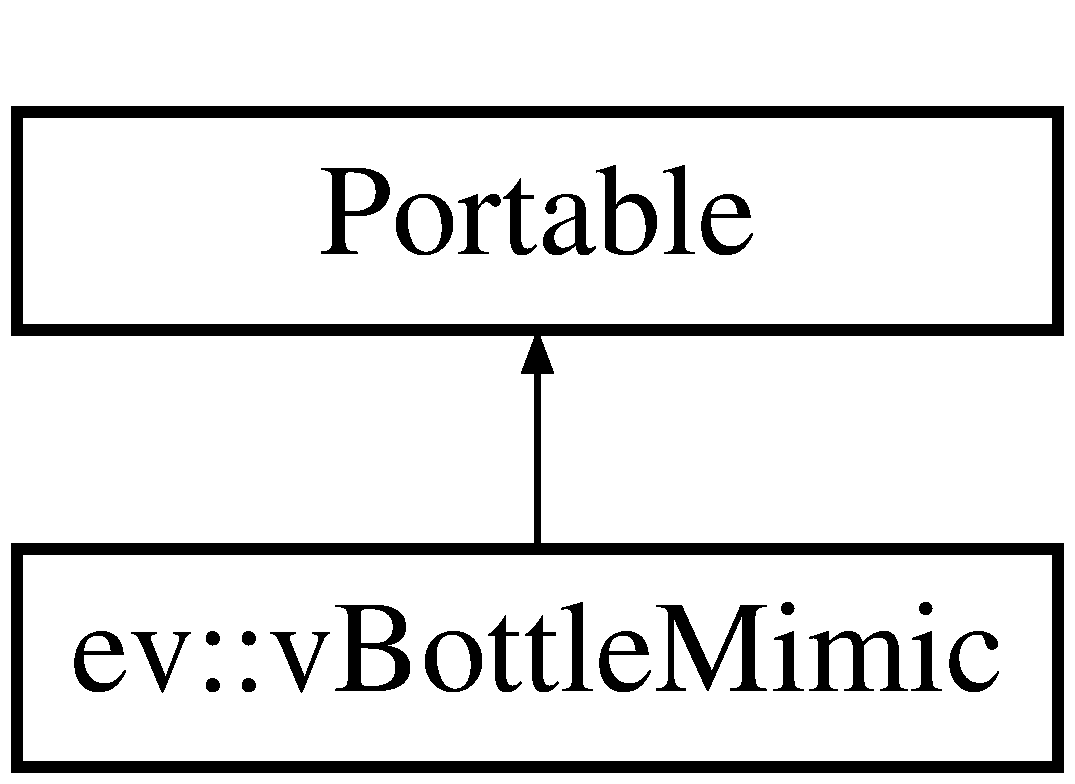
\includegraphics[height=2.000000cm]{classev_1_1vBottleMimic}
\end{center}
\end{figure}
\subsection*{Public Member Functions}
\begin{DoxyCompactItemize}
\item 
\mbox{\Hypertarget{classev_1_1vBottleMimic_ae7a95df35d75378e949ceff50d169ddf}\label{classev_1_1vBottleMimic_ae7a95df35d75378e949ceff50d169ddf}} 
\hyperlink{classev_1_1vBottleMimic_ae7a95df35d75378e949ceff50d169ddf}{v\+Bottle\+Mimic} ()
\begin{DoxyCompactList}\small\item\em instantiate the correct headers for a Bottle \end{DoxyCompactList}\item 
\mbox{\Hypertarget{classev_1_1vBottleMimic_ac3e34609dfb06ed5c10509741751c053}\label{classev_1_1vBottleMimic_ac3e34609dfb06ed5c10509741751c053}} 
void \hyperlink{classev_1_1vBottleMimic_ac3e34609dfb06ed5c10509741751c053}{set\+External\+Data} (const char $\ast$datablock, unsigned int datalength)
\begin{DoxyCompactList}\small\item\em for data already allocated in contiguous space. Just send this data on a port without memory reallocation. \end{DoxyCompactList}\item 
\mbox{\Hypertarget{classev_1_1vBottleMimic_ae32460f8fb474c394171f783d9e4aba1}\label{classev_1_1vBottleMimic_ae32460f8fb474c394171f783d9e4aba1}} 
void \hyperlink{classev_1_1vBottleMimic_ae32460f8fb474c394171f783d9e4aba1}{set\+Internal\+Data} (const v\+Queue \&q)
\begin{DoxyCompactList}\small\item\em send an entire v\+Queue. The queue is encoded and allocated into a single contiguous memory space. Faster than a standard \hyperlink{classev_1_1vBottle}{v\+Bottle}. \end{DoxyCompactList}\item 
\mbox{\Hypertarget{classev_1_1vBottleMimic_ac0f5995820702df0aea2ede33d65cace}\label{classev_1_1vBottleMimic_ac0f5995820702df0aea2ede33d65cace}} 
void \hyperlink{classev_1_1vBottleMimic_ac0f5995820702df0aea2ede33d65cace}{set\+Header} (std\+::string eventtype)
\begin{DoxyCompactList}\small\item\em set the type of event that this \hyperlink{classev_1_1vBottleMimic}{v\+Bottle\+Mimic} will send \end{DoxyCompactList}\item 
\mbox{\Hypertarget{classev_1_1vBottleMimic_a5c7ead7b0484b9abe99e922196c074ff}\label{classev_1_1vBottleMimic_a5c7ead7b0484b9abe99e922196c074ff}} 
virtual bool \hyperlink{classev_1_1vBottleMimic_a5c7ead7b0484b9abe99e922196c074ff}{read} (yarp\+::os\+::\+Connection\+Reader \&connection)
\begin{DoxyCompactList}\small\item\em does nothing as this is a write-\/only port. \end{DoxyCompactList}\item 
\mbox{\Hypertarget{classev_1_1vBottleMimic_a70d7add0350d3254f6867a3dd7f6c50b}\label{classev_1_1vBottleMimic_a70d7add0350d3254f6867a3dd7f6c50b}} 
virtual bool \hyperlink{classev_1_1vBottleMimic_a70d7add0350d3254f6867a3dd7f6c50b}{write} (yarp\+::os\+::\+Connection\+Writer \&connection) const
\begin{DoxyCompactList}\small\item\em write the data on the connection. \end{DoxyCompactList}\end{DoxyCompactItemize}


\subsection{Detailed Description}
a \hyperlink{classev_1_1vBottle}{v\+Bottle} that avoids memory allocation where possible and can be correctly decoded when read from a receiving port. Only works with a single event-\/type. 

The documentation for this class was generated from the following file\+:\begin{DoxyCompactItemize}
\item 
/mnt/d/projects/event-\/driven/lib/include/event-\/driven/v\+Bottle.\+h\end{DoxyCompactItemize}

\hypertarget{classev_1_1vDraw}{}\section{ev\+:\+:v\+Draw Class Reference}
\label{classev_1_1vDraw}\index{ev\+::v\+Draw@{ev\+::v\+Draw}}


The \hyperlink{classev_1_1vDraw}{v\+Draw} class is the base class from which all v\+Drawers should inherit. It contains the draw and get\+Tag functions which must be overloaded, and the sensor size for reference.  




{\ttfamily \#include $<$v\+Draw.\+h$>$}

Inheritance diagram for ev\+:\+:v\+Draw\+:\begin{figure}[H]
\begin{center}
\leavevmode
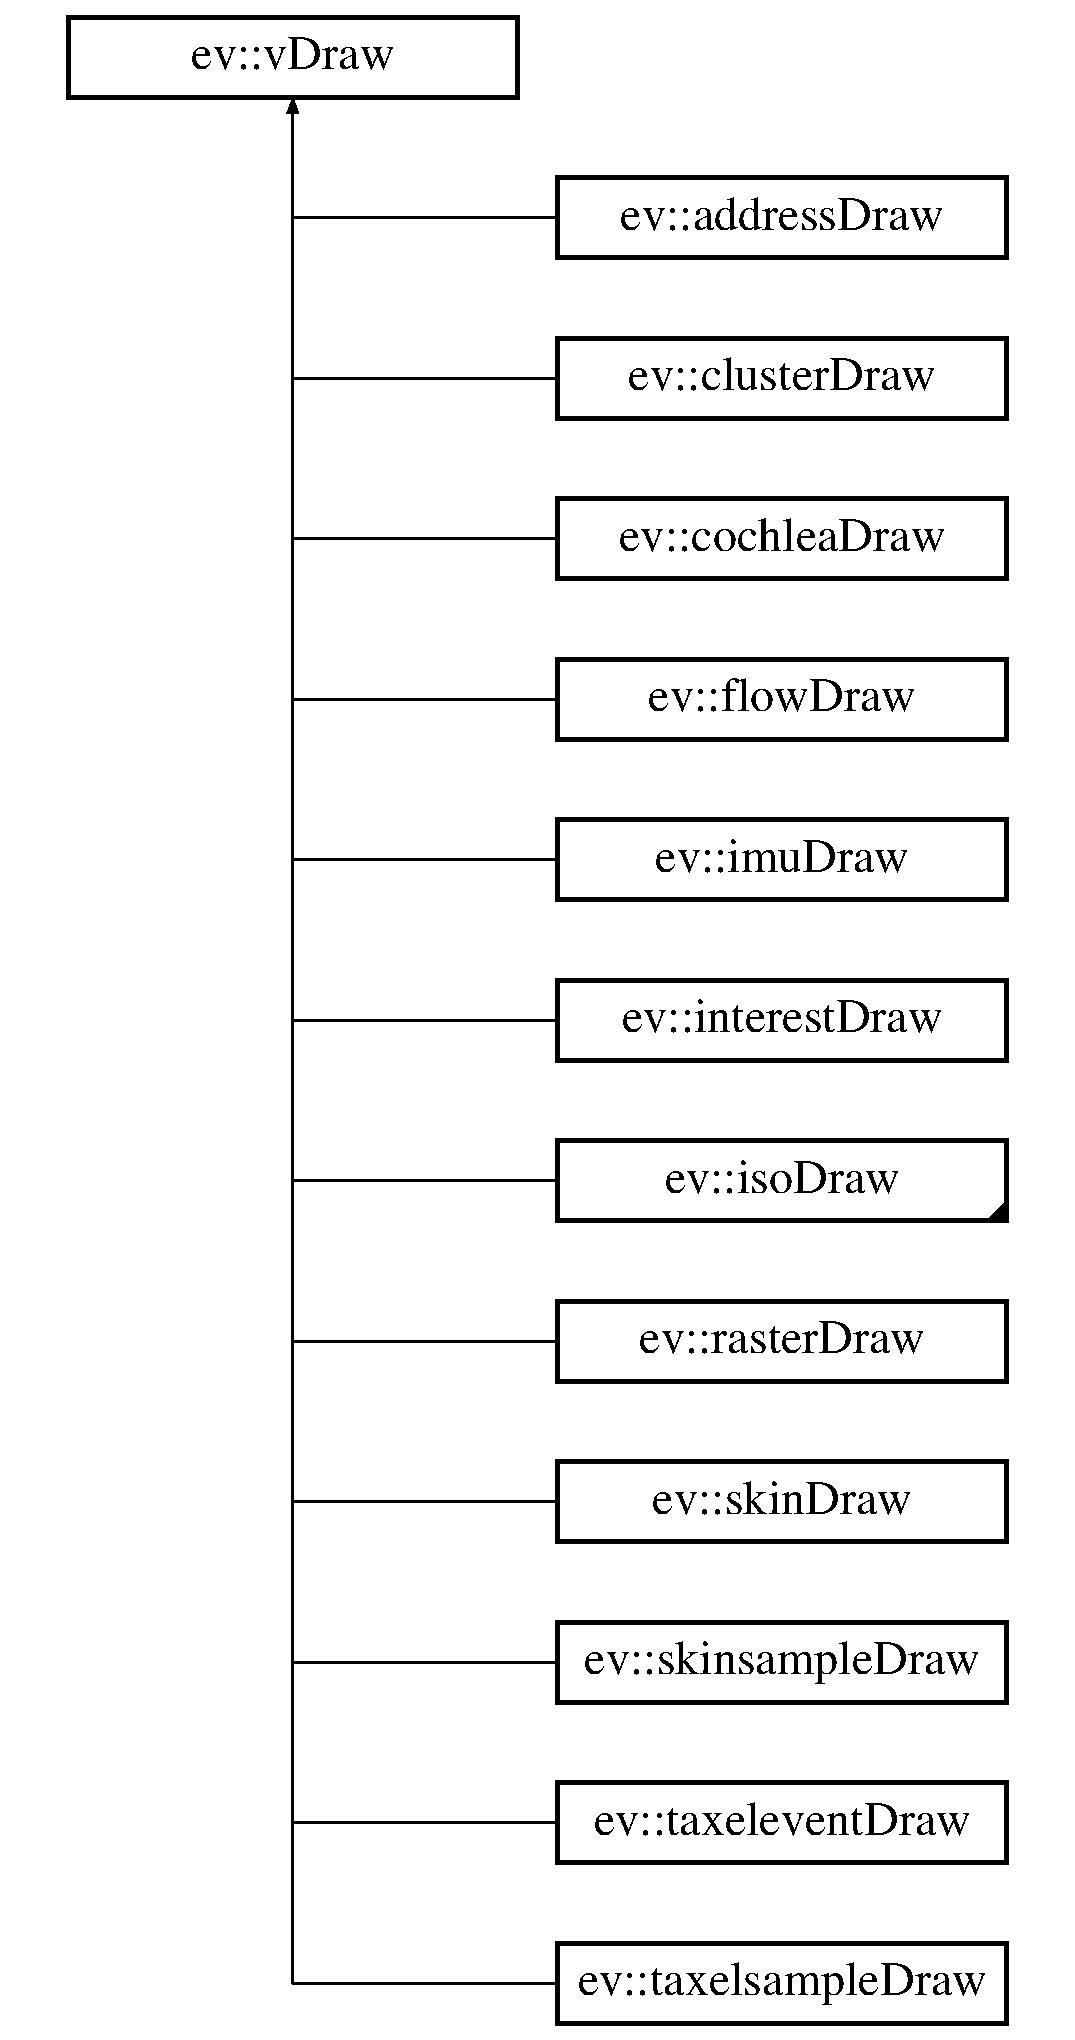
\includegraphics[height=12.000000cm]{classev_1_1vDraw}
\end{center}
\end{figure}
\subsection*{Public Member Functions}
\begin{DoxyCompactItemize}
\item 
void \hyperlink{classev_1_1vDraw_a0362710d8ca805d19b013818660bc867}{set\+Retina\+Limits} (int Xlimit, int Ylimit)
\begin{DoxyCompactList}\small\item\em set\+Limits sets the maximum possible values of the position of events that could be drawn (mostly governed by the sensor size). \end{DoxyCompactList}\item 
\mbox{\Hypertarget{classev_1_1vDraw_a67241ea174704ad575646713fc045b17}\label{classev_1_1vDraw_a67241ea174704ad575646713fc045b17}} 
void {\bfseries set\+Temporal\+Limits} (unsigned int display\+\_\+window, unsigned int max\+\_\+window)
\item 
\mbox{\Hypertarget{classev_1_1vDraw_a82a972ba5dd41bcaaffa2565bd400e89}\label{classev_1_1vDraw_a82a972ba5dd41bcaaffa2565bd400e89}} 
void {\bfseries set\+Flip} (bool flip)
\item 
\mbox{\Hypertarget{classev_1_1vDraw_ad4370892e94e8dafcc763addf50bd164}\label{classev_1_1vDraw_ad4370892e94e8dafcc763addf50bd164}} 
virtual void {\bfseries initialise} ()
\item 
\mbox{\Hypertarget{classev_1_1vDraw_a98e3b5b7114c777f4e02351b86cc7d75}\label{classev_1_1vDraw_a98e3b5b7114c777f4e02351b86cc7d75}} 
virtual void {\bfseries reset\+Image} (cv\+::\+Mat \&image)
\item 
virtual void \hyperlink{classev_1_1vDraw_af1eee5dcdf3b4cfee6a3024e5cd706f8}{draw} (cv\+::\+Mat \&canvas, const ev\+::v\+Queue \&e\+Set, int v\+Time)=0
\begin{DoxyCompactList}\small\item\em draw takes an image and overlays the new visualisation textures \end{DoxyCompactList}\item 
virtual std\+::string \hyperlink{classev_1_1vDraw_ac01381befeffef2b930cbceb28b18a28}{get\+Draw\+Type} ()=0
\begin{DoxyCompactList}\small\item\em get\+Tag returns the unique code for this drawing method. The arguments given on the command line must match this code exactly \end{DoxyCompactList}\item 
\mbox{\Hypertarget{classev_1_1vDraw_a0f9ef3a3f08b34cc0952c16329181d75}\label{classev_1_1vDraw_a0f9ef3a3f08b34cc0952c16329181d75}} 
virtual std\+::string {\bfseries get\+Event\+Type} ()=0
\end{DoxyCompactItemize}
\subsection*{Protected Attributes}
\begin{DoxyCompactItemize}
\item 
\mbox{\Hypertarget{classev_1_1vDraw_abb01af9562deeee5c654819da8f8ed48}\label{classev_1_1vDraw_abb01af9562deeee5c654819da8f8ed48}} 
int {\bfseries Xlimit}
\item 
\mbox{\Hypertarget{classev_1_1vDraw_ac8576f64274527917d90b3bd366d30cb}\label{classev_1_1vDraw_ac8576f64274527917d90b3bd366d30cb}} 
int {\bfseries Ylimit}
\item 
\mbox{\Hypertarget{classev_1_1vDraw_a1b39d618b4b05ae1af7c1f244ade51fc}\label{classev_1_1vDraw_a1b39d618b4b05ae1af7c1f244ade51fc}} 
unsigned int {\bfseries display\+\_\+window}
\item 
\mbox{\Hypertarget{classev_1_1vDraw_a3f0d8becb738e2c5b8f1035de3a68ec4}\label{classev_1_1vDraw_a3f0d8becb738e2c5b8f1035de3a68ec4}} 
unsigned int {\bfseries max\+\_\+window}
\item 
\mbox{\Hypertarget{classev_1_1vDraw_a35a10630b77794a8275e5fa1ba211c28}\label{classev_1_1vDraw_a35a10630b77794a8275e5fa1ba211c28}} 
bool {\bfseries flip}
\item 
\mbox{\Hypertarget{classev_1_1vDraw_ae6064a6b7d3e7ceac8c25023f65df312}\label{classev_1_1vDraw_ae6064a6b7d3e7ceac8c25023f65df312}} 
cv\+::\+Vec3b {\bfseries aqua} \{151, 174, 6\}
\item 
\mbox{\Hypertarget{classev_1_1vDraw_a70ac397a8d4cbea13fc6935bf1b15ef5}\label{classev_1_1vDraw_a70ac397a8d4cbea13fc6935bf1b15ef5}} 
cv\+::\+Vec3b {\bfseries violet} \{180, 10, 155\}
\item 
\mbox{\Hypertarget{classev_1_1vDraw_a1076d8ade59f536f331a32c4f01741cc}\label{classev_1_1vDraw_a1076d8ade59f536f331a32c4f01741cc}} 
cv\+::\+Vec3b {\bfseries orange} \{9, 111, 255\}
\item 
\mbox{\Hypertarget{classev_1_1vDraw_a89d68710f6031add1a4fc1b152b49a73}\label{classev_1_1vDraw_a89d68710f6031add1a4fc1b152b49a73}} 
cv\+::\+Vec3b {\bfseries lime} \{9, 250, 222\}
\item 
\mbox{\Hypertarget{classev_1_1vDraw_aa6e44598c13ee4f84d40b85416d5d5a7}\label{classev_1_1vDraw_aa6e44598c13ee4f84d40b85416d5d5a7}} 
cv\+::\+Vec3b {\bfseries white} \{255, 255, 255\}
\item 
\mbox{\Hypertarget{classev_1_1vDraw_a7b5f1fc47b30fed175f258447adc8cc4}\label{classev_1_1vDraw_a7b5f1fc47b30fed175f258447adc8cc4}} 
cv\+::\+Vec3b {\bfseries black} \{0, 0, 0\}
\item 
\mbox{\Hypertarget{classev_1_1vDraw_a00d2b2e84b9ea5bf0ee3a04cd613d22a}\label{classev_1_1vDraw_a00d2b2e84b9ea5bf0ee3a04cd613d22a}} 
cv\+::\+Vec3b {\bfseries red} \{0, 0, 255\}
\end{DoxyCompactItemize}


\subsection{Detailed Description}
The \hyperlink{classev_1_1vDraw}{v\+Draw} class is the base class from which all v\+Drawers should inherit. It contains the draw and get\+Tag functions which must be overloaded, and the sensor size for reference. 

\subsection{Member Function Documentation}
\mbox{\Hypertarget{classev_1_1vDraw_af1eee5dcdf3b4cfee6a3024e5cd706f8}\label{classev_1_1vDraw_af1eee5dcdf3b4cfee6a3024e5cd706f8}} 
\index{ev\+::v\+Draw@{ev\+::v\+Draw}!draw@{draw}}
\index{draw@{draw}!ev\+::v\+Draw@{ev\+::v\+Draw}}
\subsubsection{\texorpdfstring{draw()}{draw()}}
{\footnotesize\ttfamily virtual void ev\+::v\+Draw\+::draw (\begin{DoxyParamCaption}\item[{cv\+::\+Mat \&}]{canvas,  }\item[{const ev\+::v\+Queue \&}]{e\+Set,  }\item[{int}]{v\+Time }\end{DoxyParamCaption})\hspace{0.3cm}{\ttfamily [pure virtual]}}



draw takes an image and overlays the new visualisation textures 


\begin{DoxyParams}{Parameters}
{\em canvas} & is the image which may or may not yet exist \\
\hline
{\em e\+Set} & is the set of events which could possibly be drawn \\
\hline
\end{DoxyParams}


Implemented in \hyperlink{classev_1_1taxeleventDraw_ad2ff0348ee1b362e3c50508ffefdf9d1}{ev\+::taxelevent\+Draw}, \hyperlink{classev_1_1taxelsampleDraw_a43e40e8cfc4ed342f8d616eb9ddecf0a}{ev\+::taxelsample\+Draw}, \hyperlink{classev_1_1skinsampleDraw_a1c2492038e7fe94fe88d2286ac18f2c6}{ev\+::skinsample\+Draw}, \hyperlink{classev_1_1skinDraw_a4cbf578dd04c6a634c8959fea7295060}{ev\+::skin\+Draw}, \hyperlink{classev_1_1isoDrawSkin_a2d4ed05b06bea443974f5b07a4d69374}{ev\+::iso\+Draw\+Skin}, \hyperlink{classev_1_1isoInterestDraw_a3276f946c09d4cd0009f8379ea24d409}{ev\+::iso\+Interest\+Draw}, \hyperlink{classev_1_1clusterDraw_aa70978bb98c7bde912eb03288f21cbb5}{ev\+::cluster\+Draw}, \hyperlink{classev_1_1interestDraw_aeca2c7248d34d6817e853aad6a254380}{ev\+::interest\+Draw}, \hyperlink{classev_1_1flowDraw_a15d97ddaf93734a912be64fb60977ee2}{ev\+::flow\+Draw}, \hyperlink{classev_1_1cochleaDraw_a2b06c53991065506fcdaa9afec8282af}{ev\+::cochlea\+Draw}, \hyperlink{classev_1_1rasterDraw_a0cc698fe53b645a8a1ed8cdb40c8b7a9}{ev\+::raster\+Draw}, \hyperlink{classev_1_1imuDraw_addbaf0eff95fe6e791ca53c36218267e}{ev\+::imu\+Draw}, \hyperlink{classev_1_1addressDraw_a9ff5e558766f8b6cec2b11a60907b455}{ev\+::address\+Draw}, and \hyperlink{classev_1_1isoDraw_ad481b618ae2d08664481ffc4b3c4dd95}{ev\+::iso\+Draw}.

\mbox{\Hypertarget{classev_1_1vDraw_ac01381befeffef2b930cbceb28b18a28}\label{classev_1_1vDraw_ac01381befeffef2b930cbceb28b18a28}} 
\index{ev\+::v\+Draw@{ev\+::v\+Draw}!get\+Draw\+Type@{get\+Draw\+Type}}
\index{get\+Draw\+Type@{get\+Draw\+Type}!ev\+::v\+Draw@{ev\+::v\+Draw}}
\subsubsection{\texorpdfstring{get\+Draw\+Type()}{getDrawType()}}
{\footnotesize\ttfamily virtual std\+::string ev\+::v\+Draw\+::get\+Draw\+Type (\begin{DoxyParamCaption}{ }\end{DoxyParamCaption})\hspace{0.3cm}{\ttfamily [pure virtual]}}



get\+Tag returns the unique code for this drawing method. The arguments given on the command line must match this code exactly 

\begin{DoxyReturn}{Returns}
the tag code 
\end{DoxyReturn}


Implemented in \hyperlink{classev_1_1taxeleventDraw_a474b409ea48a97749caaf172f5fd467a}{ev\+::taxelevent\+Draw}, \hyperlink{classev_1_1taxelsampleDraw_a7bf19e7de1e4851b5567308e95334942}{ev\+::taxelsample\+Draw}, \hyperlink{classev_1_1skinsampleDraw_a32064d959f2c127d25a9fa6773384850}{ev\+::skinsample\+Draw}, \hyperlink{classev_1_1skinDraw_a7015a083dffe5c055808c20b9372bce4}{ev\+::skin\+Draw}, \hyperlink{classev_1_1isoDrawSkin_a9f1bce77ba050a37dfe151e2246779bc}{ev\+::iso\+Draw\+Skin}, \hyperlink{classev_1_1isoInterestDraw_a93b2142d5652f725e21d34fedde103df}{ev\+::iso\+Interest\+Draw}, \hyperlink{classev_1_1clusterDraw_a21cd4ba2277ad5258b39d135e445b32f}{ev\+::cluster\+Draw}, \hyperlink{classev_1_1interestDraw_a97dbea009b993f0d8f4b6967b2b241ad}{ev\+::interest\+Draw}, \hyperlink{classev_1_1flowDraw_a6caf6d848d79407e62b7bf13c58d583e}{ev\+::flow\+Draw}, \hyperlink{classev_1_1cochleaDraw_a722aac2b6c1af1f6691721beb8a25325}{ev\+::cochlea\+Draw}, \hyperlink{classev_1_1rasterDraw_a687569e3beafa6aa9e73e3eeaad64d59}{ev\+::raster\+Draw}, \hyperlink{classev_1_1imuDraw_ab622b53cbe53421958cb7572919a0318}{ev\+::imu\+Draw}, \hyperlink{classev_1_1addressDraw_a92e98d08d1fdbf47d7e0cb9fcf7a9937}{ev\+::address\+Draw}, and \hyperlink{classev_1_1isoDraw_abd32cc393e5489ee97b5a8b94e6dd88d}{ev\+::iso\+Draw}.

\mbox{\Hypertarget{classev_1_1vDraw_a0362710d8ca805d19b013818660bc867}\label{classev_1_1vDraw_a0362710d8ca805d19b013818660bc867}} 
\index{ev\+::v\+Draw@{ev\+::v\+Draw}!set\+Retina\+Limits@{set\+Retina\+Limits}}
\index{set\+Retina\+Limits@{set\+Retina\+Limits}!ev\+::v\+Draw@{ev\+::v\+Draw}}
\subsubsection{\texorpdfstring{set\+Retina\+Limits()}{setRetinaLimits()}}
{\footnotesize\ttfamily void ev\+::v\+Draw\+::set\+Retina\+Limits (\begin{DoxyParamCaption}\item[{int}]{Xlimit,  }\item[{int}]{Ylimit }\end{DoxyParamCaption})\hspace{0.3cm}{\ttfamily [inline]}}



set\+Limits sets the maximum possible values of the position of events that could be drawn (mostly governed by the sensor size). 


\begin{DoxyParams}{Parameters}
{\em Xlimit} & is the maximum x value (width) \\
\hline
{\em Ylimit} & is the maximium y value (height) \\
\hline
\end{DoxyParams}


The documentation for this class was generated from the following file\+:\begin{DoxyCompactItemize}
\item 
/mnt/d/projects/event-\/driven/lib/include/event-\/driven/v\+Draw.\+h\end{DoxyCompactItemize}

\hypertarget{classev_1_1vEdge}{}\section{ev\+:\+:v\+Edge Class Reference}
\label{classev_1_1vEdge}\index{ev\+::v\+Edge@{ev\+::v\+Edge}}


a spatio-\/temporal surface storing events along edges as given by plane fitting  




{\ttfamily \#include $<$v\+Window\+\_\+adv.\+h$>$}

Inheritance diagram for ev\+:\+:v\+Edge\+:\begin{figure}[H]
\begin{center}
\leavevmode
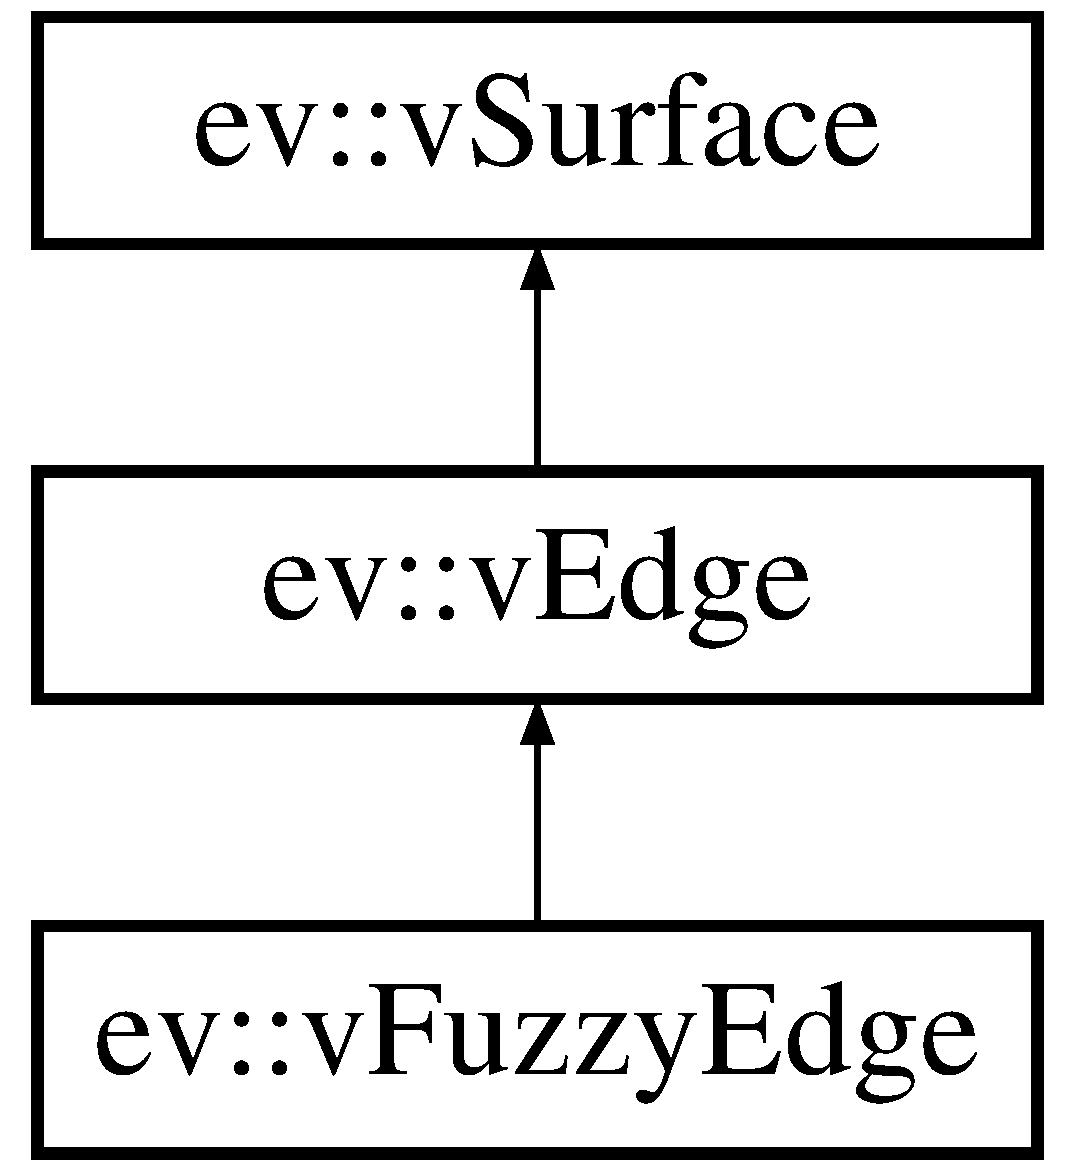
\includegraphics[height=3.000000cm]{classev_1_1vEdge}
\end{center}
\end{figure}
\subsection*{Public Member Functions}
\begin{DoxyCompactItemize}
\item 
\mbox{\Hypertarget{classev_1_1vEdge_a3bbccb1784adbb0543a22e6e1a805be5}\label{classev_1_1vEdge_a3bbccb1784adbb0543a22e6e1a805be5}} 
{\bfseries v\+Edge} (int width=128, int height=128)
\item 
\mbox{\Hypertarget{classev_1_1vEdge_a04bc02981fe09b9cc0615a471a4d1594}\label{classev_1_1vEdge_a04bc02981fe09b9cc0615a471a4d1594}} 
v\+Queue {\bfseries add\+Event\+To\+Edge} (event$<$ \hyperlink{classev_1_1AddressEvent}{Address\+Event} $>$ v)
\item 
\mbox{\Hypertarget{classev_1_1vEdge_a8add033e36c36c4145d932d8e210750a}\label{classev_1_1vEdge_a8add033e36c36c4145d932d8e210750a}} 
void {\bfseries set\+Thickness} (int pixels)
\item 
\mbox{\Hypertarget{classev_1_1vEdge_a7e0dd1c7f362d79a0cef3298caa74f8a}\label{classev_1_1vEdge_a7e0dd1c7f362d79a0cef3298caa74f8a}} 
void {\bfseries track} (bool track\+Count=true)
\item 
\mbox{\Hypertarget{classev_1_1vEdge_a569d6c449ae172b608c0049e9e391e50}\label{classev_1_1vEdge_a569d6c449ae172b608c0049e9e391e50}} 
virtual const v\+Queue {\bfseries get\+Surf} (int xl, int xh, int yl, int yh)
\end{DoxyCompactItemize}
\subsection*{Additional Inherited Members}


\subsection{Detailed Description}
a spatio-\/temporal surface storing events along edges as given by plane fitting 

The documentation for this class was generated from the following files\+:\begin{DoxyCompactItemize}
\item 
/mnt/d/projects/event-\/driven/lib/include/event-\/driven/v\+Window\+\_\+adv.\+h\item 
/mnt/d/projects/event-\/driven/lib/src/v\+Window\+\_\+adv.\+cpp\end{DoxyCompactItemize}

\hypertarget{classev_1_1vEvent}{}\section{ev\+:\+:v\+Event Class Reference}
\label{classev_1_1vEvent}\index{ev\+::v\+Event@{ev\+::v\+Event}}


base event class which defines the time the event occurs  




{\ttfamily \#include $<$v\+Codec.\+h$>$}

Inheritance diagram for ev\+:\+:v\+Event\+:\begin{figure}[H]
\begin{center}
\leavevmode
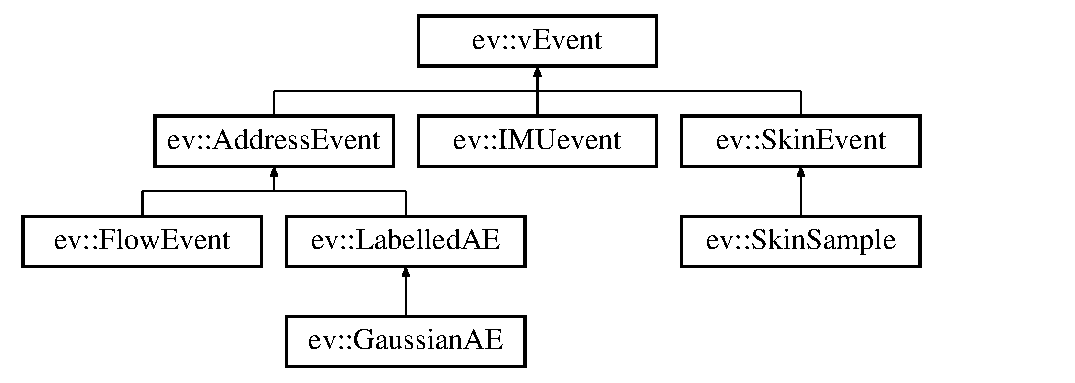
\includegraphics[height=4.000000cm]{classev_1_1vEvent}
\end{center}
\end{figure}
\subsection*{Public Member Functions}
\begin{DoxyCompactItemize}
\item 
\mbox{\Hypertarget{classev_1_1vEvent_a44f88f43a5c6b5aa6d93001a11f9309b}\label{classev_1_1vEvent_a44f88f43a5c6b5aa6d93001a11f9309b}} 
virtual event {\bfseries clone} ()
\item 
\mbox{\Hypertarget{classev_1_1vEvent_a1c817535c284d50449df9a12e085933b}\label{classev_1_1vEvent_a1c817535c284d50449df9a12e085933b}} 
virtual void {\bfseries encode} (yarp\+::os\+::\+Bottle \&b) const
\item 
\mbox{\Hypertarget{classev_1_1vEvent_a59f6e08e4faa7ae72aa8449a15340f29}\label{classev_1_1vEvent_a59f6e08e4faa7ae72aa8449a15340f29}} 
virtual void {\bfseries encode} (std\+::vector$<$ int32\+\_\+t $>$ \&b, unsigned int \&pos) const
\item 
\mbox{\Hypertarget{classev_1_1vEvent_a86e3212efa43423bff4c2bf25434066f}\label{classev_1_1vEvent_a86e3212efa43423bff4c2bf25434066f}} 
virtual bool {\bfseries decode} (const yarp\+::os\+::\+Bottle \&packet, size\+\_\+t \&pos)
\item 
\mbox{\Hypertarget{classev_1_1vEvent_a889831584c53a9d14b1a68dfbccf5a6a}\label{classev_1_1vEvent_a889831584c53a9d14b1a68dfbccf5a6a}} 
virtual void {\bfseries decode} (const int32\+\_\+t $\ast$\&data)
\item 
\mbox{\Hypertarget{classev_1_1vEvent_a02fb3afb67cf6ff38fa63d1ce8ef12a3}\label{classev_1_1vEvent_a02fb3afb67cf6ff38fa63d1ce8ef12a3}} 
virtual yarp\+::os\+::\+Property {\bfseries get\+Content} () const
\item 
\mbox{\Hypertarget{classev_1_1vEvent_aeb99e71fbb8e8aa21e911de146768aba}\label{classev_1_1vEvent_aeb99e71fbb8e8aa21e911de146768aba}} 
virtual std\+::string {\bfseries get\+Type} () const
\item 
\mbox{\Hypertarget{classev_1_1vEvent_aa427d1e35f2b762f39820b113377d30c}\label{classev_1_1vEvent_aa427d1e35f2b762f39820b113377d30c}} 
virtual int {\bfseries get\+Channel} () const
\item 
\mbox{\Hypertarget{classev_1_1vEvent_a2cf5bf1d01ad2757a82b6e07d7e2a5da}\label{classev_1_1vEvent_a2cf5bf1d01ad2757a82b6e07d7e2a5da}} 
virtual void {\bfseries set\+Channel} ()
\end{DoxyCompactItemize}
\subsection*{Public Attributes}
\begin{DoxyCompactItemize}
\item 
\mbox{\Hypertarget{classev_1_1vEvent_ad4e003653fa59b37682addefce835490}\label{classev_1_1vEvent_ad4e003653fa59b37682addefce835490}} 
unsigned int {\bfseries stamp}\+:31
\end{DoxyCompactItemize}
\subsection*{Static Public Attributes}
\begin{DoxyCompactItemize}
\item 
\mbox{\Hypertarget{classev_1_1vEvent_a54bcc0830c5993b56f1f47e23df1de8e}\label{classev_1_1vEvent_a54bcc0830c5993b56f1f47e23df1de8e}} 
static const std\+::string {\bfseries tag} = \char`\"{}TS\char`\"{}
\end{DoxyCompactItemize}


\subsection{Detailed Description}
base event class which defines the time the event occurs 

The documentation for this class was generated from the following files\+:\begin{DoxyCompactItemize}
\item 
/mnt/d/projects/event-\/driven/lib/include/event-\/driven/v\+Codec.\+h\item 
/mnt/d/projects/event-\/driven/lib/src/codecs/codec\+\_\+v\+Event.\+cpp\end{DoxyCompactItemize}

\hypertarget{classev_1_1vFuzzyEdge}{}\section{ev\+:\+:v\+Fuzzy\+Edge Class Reference}
\label{classev_1_1vFuzzyEdge}\index{ev\+::v\+Fuzzy\+Edge@{ev\+::v\+Fuzzy\+Edge}}


a \hyperlink{classev_1_1vEdge}{v\+Edge} structure that keeps events given a \char`\"{}fuzzy\char`\"{} scoring system  




{\ttfamily \#include $<$v\+Window\+\_\+adv.\+h$>$}

Inheritance diagram for ev\+:\+:v\+Fuzzy\+Edge\+:\begin{figure}[H]
\begin{center}
\leavevmode
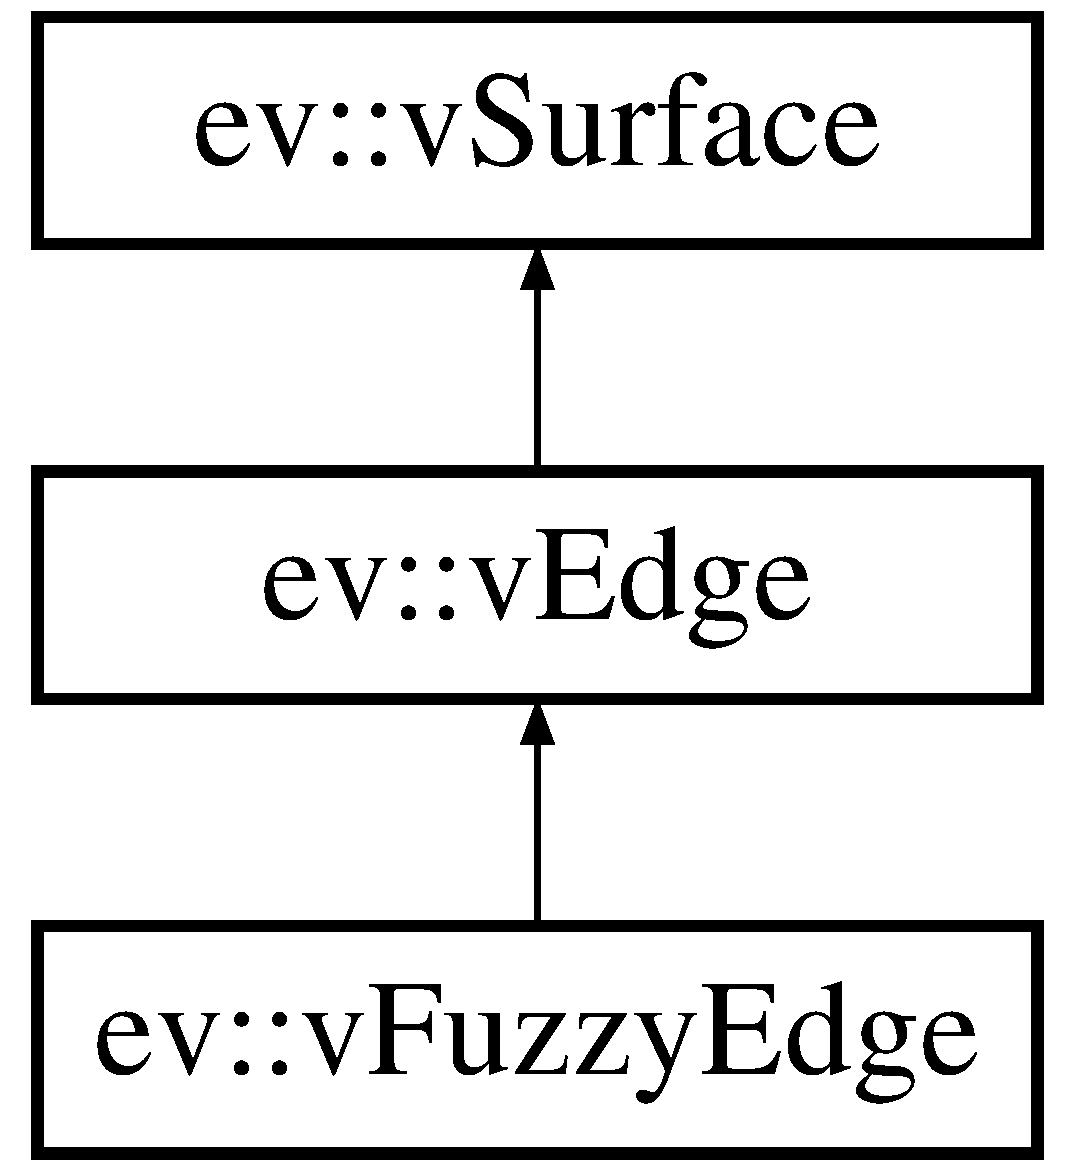
\includegraphics[height=3.000000cm]{classev_1_1vFuzzyEdge}
\end{center}
\end{figure}
\subsection*{Public Member Functions}
\begin{DoxyCompactItemize}
\item 
\mbox{\Hypertarget{classev_1_1vFuzzyEdge_a4fa6e20618a528a591baf2f098cace53}\label{classev_1_1vFuzzyEdge_a4fa6e20618a528a591baf2f098cace53}} 
{\bfseries v\+Fuzzy\+Edge} (int width=128, int height=128, double delta=0.\+4)
\item 
\mbox{\Hypertarget{classev_1_1vFuzzyEdge_a61803b783119945df5c130c12d99e9c2}\label{classev_1_1vFuzzyEdge_a61803b783119945df5c130c12d99e9c2}} 
v\+Queue {\bfseries add\+Event\+To\+Edge} (event$<$ \hyperlink{classev_1_1AddressEvent}{Address\+Event} $>$ event)
\item 
\mbox{\Hypertarget{classev_1_1vFuzzyEdge_a335aeb48314d3e2068a55ee0a6958643}\label{classev_1_1vFuzzyEdge_a335aeb48314d3e2068a55ee0a6958643}} 
virtual const v\+Queue {\bfseries get\+S\+U\+RF} (int xl, int xh, int yl, int yh)
\end{DoxyCompactItemize}
\subsection*{Additional Inherited Members}


\subsection{Detailed Description}
a \hyperlink{classev_1_1vEdge}{v\+Edge} structure that keeps events given a \char`\"{}fuzzy\char`\"{} scoring system 

The documentation for this class was generated from the following files\+:\begin{DoxyCompactItemize}
\item 
/mnt/d/projects/event-\/driven/lib/include/event-\/driven/v\+Window\+\_\+adv.\+h\item 
/mnt/d/projects/event-\/driven/lib/src/v\+Window\+\_\+adv.\+cpp\end{DoxyCompactItemize}

\hypertarget{classev_1_1vIPT}{}\section{ev\+:\+:v\+I\+PT Class Reference}
\label{classev_1_1vIPT}\index{ev\+::v\+I\+PT@{ev\+::v\+I\+PT}}
\subsection*{Public Member Functions}
\begin{DoxyCompactItemize}
\item 
\mbox{\Hypertarget{classev_1_1vIPT_a3ba2129509fc6405990cd138ebabde0d}\label{classev_1_1vIPT_a3ba2129509fc6405990cd138ebabde0d}} 
void {\bfseries set\+Projected\+Image\+Size} (int height, int width)
\item 
\mbox{\Hypertarget{classev_1_1vIPT_a0e2d87532a04fd0ba19464133d7df292}\label{classev_1_1vIPT_a0e2d87532a04fd0ba19464133d7df292}} 
bool {\bfseries configure} (const std\+::string calib\+Context, const std\+::string calib\+File, int size\+\_\+scaler=2)
\item 
\mbox{\Hypertarget{classev_1_1vIPT_ab946ef3a96b37185ce14b578641673ad}\label{classev_1_1vIPT_ab946ef3a96b37185ce14b578641673ad}} 
bool {\bfseries show\+Map\+Projections} (double seconds=0)
\item 
\mbox{\Hypertarget{classev_1_1vIPT_a15a9b59129f7dc5d56f2164a33853bb4}\label{classev_1_1vIPT_a15a9b59129f7dc5d56f2164a33853bb4}} 
void {\bfseries show\+Mono\+Projections} (int cam, double seconds)
\item 
\mbox{\Hypertarget{classev_1_1vIPT_ab607f86eec5f5147d5940293c298ac87}\label{classev_1_1vIPT_ab607f86eec5f5147d5940293c298ac87}} 
bool {\bfseries sparse\+Forward\+Transform} (int cam, int \&y, int \&x)
\item 
\mbox{\Hypertarget{classev_1_1vIPT_af75a5bb46e8a8c17146a00cd38530c83}\label{classev_1_1vIPT_af75a5bb46e8a8c17146a00cd38530c83}} 
bool {\bfseries sparse\+Reverse\+Transform} (int cam, int \&y, int \&x)
\item 
\mbox{\Hypertarget{classev_1_1vIPT_a70d19f6494aba2f6a16f057cd53ca659}\label{classev_1_1vIPT_a70d19f6494aba2f6a16f057cd53ca659}} 
bool {\bfseries sparse\+Project\+Cam0\+To\+Cam1} (int \&y, int \&x)
\item 
\mbox{\Hypertarget{classev_1_1vIPT_a8d87fce16f963ac875c65cc21643ada5}\label{classev_1_1vIPT_a8d87fce16f963ac875c65cc21643ada5}} 
bool {\bfseries sparse\+Project\+Cam1\+To\+Cam0} (int \&y, int \&x)
\item 
\mbox{\Hypertarget{classev_1_1vIPT_aeea8f19d5e518a6f5c4b183ac9b77f8d}\label{classev_1_1vIPT_aeea8f19d5e518a6f5c4b183ac9b77f8d}} 
bool {\bfseries dense\+Forward\+Transform} (int cam, cv\+::\+Mat \&m)
\item 
\mbox{\Hypertarget{classev_1_1vIPT_aa783cdb93de9493965ee07a66aade258}\label{classev_1_1vIPT_aa783cdb93de9493965ee07a66aade258}} 
bool {\bfseries dense\+Reverse\+Transform} (int cam, cv\+::\+Mat \&m)
\item 
\mbox{\Hypertarget{classev_1_1vIPT_ace6abc6a89c59e3b330abac1d02703f1}\label{classev_1_1vIPT_ace6abc6a89c59e3b330abac1d02703f1}} 
bool {\bfseries dense\+Project\+Cam0\+To\+Cam1} (cv\+::\+Mat \&m)
\item 
\mbox{\Hypertarget{classev_1_1vIPT_ae17ef6d577f0aab01ac19bbe39046bf9}\label{classev_1_1vIPT_ae17ef6d577f0aab01ac19bbe39046bf9}} 
bool {\bfseries dense\+Project\+Cam1\+To\+Cam0} (cv\+::\+Mat \&m)
\end{DoxyCompactItemize}


The documentation for this class was generated from the following files\+:\begin{DoxyCompactItemize}
\item 
/mnt/d/projects/event-\/driven/lib/include/event-\/driven/v\+I\+P\+T.\+h\item 
/mnt/d/projects/event-\/driven/lib/src/v\+I\+P\+T.\+cpp\end{DoxyCompactItemize}

\hypertarget{classev_1_1vNoiseFilter}{}\section{ev\+:\+:v\+Noise\+Filter Class Reference}
\label{classev_1_1vNoiseFilter}\index{ev\+::v\+Noise\+Filter@{ev\+::v\+Noise\+Filter}}


an efficient event-\/based salt and pepper filter  




{\ttfamily \#include $<$v\+Filters.\+h$>$}

\subsection*{Public Member Functions}
\begin{DoxyCompactItemize}
\item 
\mbox{\Hypertarget{classev_1_1vNoiseFilter_a762260be3ee9eb0923fe08f906da975f}\label{classev_1_1vNoiseFilter_a762260be3ee9eb0923fe08f906da975f}} 
\hyperlink{classev_1_1vNoiseFilter_a762260be3ee9eb0923fe08f906da975f}{v\+Noise\+Filter} ()
\begin{DoxyCompactList}\small\item\em constructor \end{DoxyCompactList}\item 
\mbox{\Hypertarget{classev_1_1vNoiseFilter_a9bdcff0c39c0c0d88c763050ba69cf19}\label{classev_1_1vNoiseFilter_a9bdcff0c39c0c0d88c763050ba69cf19}} 
void \hyperlink{classev_1_1vNoiseFilter_a9bdcff0c39c0c0d88c763050ba69cf19}{initialise} (unsigned int width, unsigned int height)
\begin{DoxyCompactList}\small\item\em initialise the sensor size and the filter parameters. \end{DoxyCompactList}\item 
\mbox{\Hypertarget{classev_1_1vNoiseFilter_a9038e484f9ad53c9cf9c59f4f76a567d}\label{classev_1_1vNoiseFilter_a9038e484f9ad53c9cf9c59f4f76a567d}} 
void {\bfseries use\+\_\+temporal\+\_\+filter} (int t\+\_\+param)
\item 
\mbox{\Hypertarget{classev_1_1vNoiseFilter_a667c37cc198f5410b071bab22117dd2e}\label{classev_1_1vNoiseFilter_a667c37cc198f5410b071bab22117dd2e}} 
void {\bfseries use\+\_\+spatial\+\_\+filter} (int t\+\_\+param, unsigned int s\+\_\+param)
\item 
bool \hyperlink{classev_1_1vNoiseFilter_a8aa612fbfc163398c600853329768892}{check} (int x, int y, int p, int ts)
\begin{DoxyCompactList}\small\item\em classifies the event as noise or signal \end{DoxyCompactList}\end{DoxyCompactItemize}


\subsection{Detailed Description}
an efficient event-\/based salt and pepper filter 

\subsection{Member Function Documentation}
\mbox{\Hypertarget{classev_1_1vNoiseFilter_a8aa612fbfc163398c600853329768892}\label{classev_1_1vNoiseFilter_a8aa612fbfc163398c600853329768892}} 
\index{ev\+::v\+Noise\+Filter@{ev\+::v\+Noise\+Filter}!check@{check}}
\index{check@{check}!ev\+::v\+Noise\+Filter@{ev\+::v\+Noise\+Filter}}
\subsubsection{\texorpdfstring{check()}{check()}}
{\footnotesize\ttfamily bool ev\+::v\+Noise\+Filter\+::check (\begin{DoxyParamCaption}\item[{int}]{x,  }\item[{int}]{y,  }\item[{int}]{p,  }\item[{int}]{ts }\end{DoxyParamCaption})\hspace{0.3cm}{\ttfamily [inline]}}



classifies the event as noise or signal 

\begin{DoxyReturn}{Returns}
false if the event is noise 
\end{DoxyReturn}


The documentation for this class was generated from the following file\+:\begin{DoxyCompactItemize}
\item 
/mnt/d/projects/event-\/driven/lib/include/event-\/driven/v\+Filters.\+h\end{DoxyCompactItemize}

\hypertarget{classev_1_1vPortableInterface}{}\section{ev\+:\+:v\+Portable\+Interface Class Reference}
\label{classev_1_1vPortableInterface}\index{ev\+::v\+Portable\+Interface@{ev\+::v\+Portable\+Interface}}
Inheritance diagram for ev\+:\+:v\+Portable\+Interface\+:\begin{figure}[H]
\begin{center}
\leavevmode
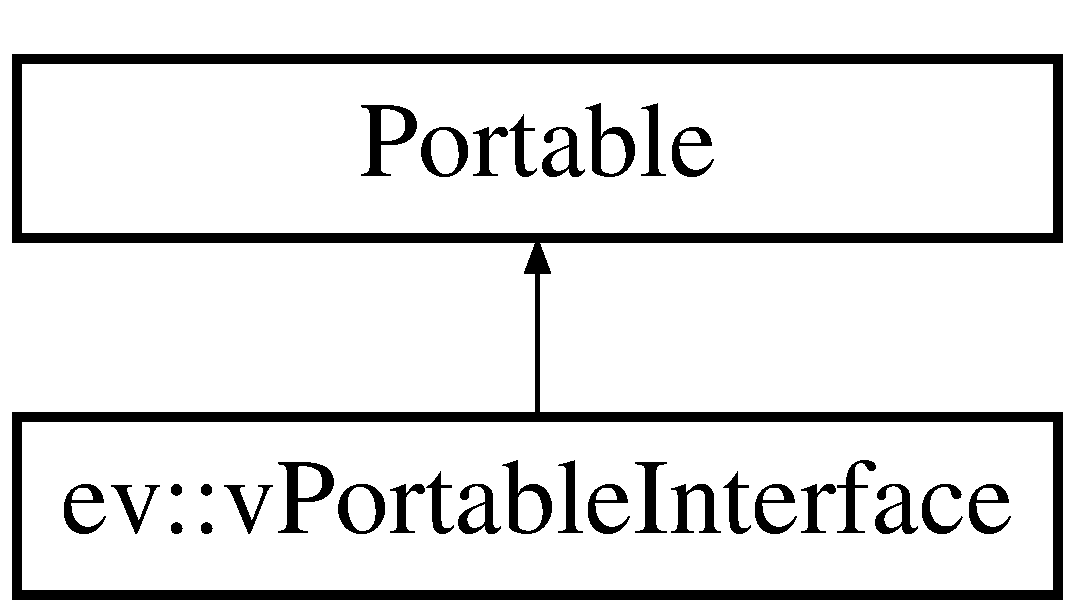
\includegraphics[height=2.000000cm]{classev_1_1vPortableInterface}
\end{center}
\end{figure}
\subsection*{Public Member Functions}
\begin{DoxyCompactItemize}
\item 
\mbox{\Hypertarget{classev_1_1vPortableInterface_a4746190970eab382c61c2711c5b40636}\label{classev_1_1vPortableInterface_a4746190970eab382c61c2711c5b40636}} 
\hyperlink{classev_1_1vPortableInterface_a4746190970eab382c61c2711c5b40636}{v\+Portable\+Interface} ()
\begin{DoxyCompactList}\small\item\em instantiate the correct headers for a Bottle \end{DoxyCompactList}\item 
\mbox{\Hypertarget{classev_1_1vPortableInterface_a4a8a2784b91e6f9e0e17ee1aee847f5d}\label{classev_1_1vPortableInterface_a4a8a2784b91e6f9e0e17ee1aee847f5d}} 
void \hyperlink{classev_1_1vPortableInterface_a4a8a2784b91e6f9e0e17ee1aee847f5d}{set\+Header} (std\+::string eventtype)
\begin{DoxyCompactList}\small\item\em set the type of event that this \hyperlink{classev_1_1vBottleMimic}{v\+Bottle\+Mimic} will send \end{DoxyCompactList}\item 
\mbox{\Hypertarget{classev_1_1vPortableInterface_aa2a6980456b48a29e92d126de656276e}\label{classev_1_1vPortableInterface_aa2a6980456b48a29e92d126de656276e}} 
void \hyperlink{classev_1_1vPortableInterface_aa2a6980456b48a29e92d126de656276e}{set\+External\+Data} (const char $\ast$datablock, unsigned int datalength)
\begin{DoxyCompactList}\small\item\em for data already allocated in contiguous space. Just send this data on a port without memory reallocation. \end{DoxyCompactList}\item 
\mbox{\Hypertarget{classev_1_1vPortableInterface_ad2dd57b8ef653984b5a52522cfddaea9}\label{classev_1_1vPortableInterface_ad2dd57b8ef653984b5a52522cfddaea9}} 
void \hyperlink{classev_1_1vPortableInterface_ad2dd57b8ef653984b5a52522cfddaea9}{set\+Internal\+Data} (const v\+Queue \&q)
\begin{DoxyCompactList}\small\item\em send an entire v\+Queue. The queue is encoded and allocated into a single contiguous memory space. Faster than a standard \hyperlink{classev_1_1vBottle}{v\+Bottle}. \end{DoxyCompactList}\item 
\mbox{\Hypertarget{classev_1_1vPortableInterface_aabd7db2eee7f3d39fe6e87023fc39ed2}\label{classev_1_1vPortableInterface_aabd7db2eee7f3d39fe6e87023fc39ed2}} 
{\footnotesize template$<$typename T $>$ }\\void \hyperlink{classev_1_1vPortableInterface_aabd7db2eee7f3d39fe6e87023fc39ed2}{set\+Internal\+Data} (const std\+::deque$<$ T $>$ \&q)
\begin{DoxyCompactList}\small\item\em send an entire v\+Queue. The queue is encoded and allocated into a single contiguous memory space. Faster than a standard \hyperlink{classev_1_1vBottle}{v\+Bottle}. \end{DoxyCompactList}\item 
\mbox{\Hypertarget{classev_1_1vPortableInterface_a86eb64481d56c34f3848d27e5cc654f0}\label{classev_1_1vPortableInterface_a86eb64481d56c34f3848d27e5cc654f0}} 
{\footnotesize template$<$typename T $>$ }\\void {\bfseries set\+Internal\+Data} (const std\+::vector$<$ T $>$ \&q)
\item 
\mbox{\Hypertarget{classev_1_1vPortableInterface_a1483ddacc49ebce50fa482cb87227ce5}\label{classev_1_1vPortableInterface_a1483ddacc49ebce50fa482cb87227ce5}} 
void {\bfseries set\+Internal\+Data} (const deque$<$ int32\+\_\+t $>$ \&q)
\item 
\mbox{\Hypertarget{classev_1_1vPortableInterface_aef6ef668c89f85168f34c7e0c05a6ced}\label{classev_1_1vPortableInterface_aef6ef668c89f85168f34c7e0c05a6ced}} 
bool \hyperlink{classev_1_1vPortableInterface_aef6ef668c89f85168f34c7e0c05a6ced}{write} (yarp\+::os\+::\+Connection\+Writer \&connection) const
\begin{DoxyCompactList}\small\item\em write the data on the connection. \end{DoxyCompactList}\item 
\mbox{\Hypertarget{classev_1_1vPortableInterface_ab402795dcf4ab5ca872b5a099197a2e4}\label{classev_1_1vPortableInterface_ab402795dcf4ab5ca872b5a099197a2e4}} 
bool \hyperlink{classev_1_1vPortableInterface_ab402795dcf4ab5ca872b5a099197a2e4}{read} (yarp\+::os\+::\+Connection\+Reader \&connection)
\begin{DoxyCompactList}\small\item\em does nothing as this is a write-\/only port. \end{DoxyCompactList}\item 
\mbox{\Hypertarget{classev_1_1vPortableInterface_ac7cd04f6a05e64ec4abe1f9322437315}\label{classev_1_1vPortableInterface_ac7cd04f6a05e64ec4abe1f9322437315}} 
bool {\bfseries decode\+Packet} (v\+Queue \&read\+\_\+q)
\item 
\mbox{\Hypertarget{classev_1_1vPortableInterface_abe80d47ae0323e6245b0e7a2aa0aac78}\label{classev_1_1vPortableInterface_abe80d47ae0323e6245b0e7a2aa0aac78}} 
{\footnotesize template$<$typename T $>$ }\\bool {\bfseries decode\+Packet} (vector$<$ T $>$ \&read\+\_\+q)
\item 
\mbox{\Hypertarget{classev_1_1vPortableInterface_acac49767e0f87e2be5185d373f629097}\label{classev_1_1vPortableInterface_acac49767e0f87e2be5185d373f629097}} 
bool {\bfseries decode\+Packet} (vector$<$ int32\+\_\+t $>$ \&read\+\_\+q)
\end{DoxyCompactItemize}
\subsection*{Public Attributes}
\begin{DoxyCompactItemize}
\item 
\mbox{\Hypertarget{classev_1_1vPortableInterface_ae8efe8cb3e40fc651d359073e6f53396}\label{classev_1_1vPortableInterface_ae8efe8cb3e40fc651d359073e6f53396}} 
vector$<$ int32\+\_\+t $>$ {\bfseries internaldata}
\end{DoxyCompactItemize}
\subsection*{Protected Attributes}
\begin{DoxyCompactItemize}
\item 
\mbox{\Hypertarget{classev_1_1vPortableInterface_aa6963fbd9f86d0c12b1cec3f50154039}\label{classev_1_1vPortableInterface_aa6963fbd9f86d0c12b1cec3f50154039}} 
vector$<$ int32\+\_\+t $>$ {\bfseries header1}
\item 
\mbox{\Hypertarget{classev_1_1vPortableInterface_aacd6a1f6ca7e75d8b56fb00bdab93115}\label{classev_1_1vPortableInterface_aacd6a1f6ca7e75d8b56fb00bdab93115}} 
string {\bfseries header2}
\item 
\mbox{\Hypertarget{classev_1_1vPortableInterface_a4c8644690c45885728ccded09831b907}\label{classev_1_1vPortableInterface_a4c8644690c45885728ccded09831b907}} 
vector$<$ int32\+\_\+t $>$ {\bfseries header3}
\item 
\mbox{\Hypertarget{classev_1_1vPortableInterface_a4e3377c27147a1dd9364a9c01a9433a3}\label{classev_1_1vPortableInterface_a4e3377c27147a1dd9364a9c01a9433a3}} 
const char $\ast$ {\bfseries datablock}
\item 
\mbox{\Hypertarget{classev_1_1vPortableInterface_afb56f5c3c78e2029796cc8e3633c7fb1}\label{classev_1_1vPortableInterface_afb56f5c3c78e2029796cc8e3633c7fb1}} 
unsigned int {\bfseries datalength}
\item 
\mbox{\Hypertarget{classev_1_1vPortableInterface_a74417dedd31327a04fcb03f9c5362651}\label{classev_1_1vPortableInterface_a74417dedd31327a04fcb03f9c5362651}} 
string {\bfseries event\+\_\+type}
\item 
\mbox{\Hypertarget{classev_1_1vPortableInterface_a9f1790f33d34109839ad9845dffb6e77}\label{classev_1_1vPortableInterface_a9f1790f33d34109839ad9845dffb6e77}} 
unsigned int {\bfseries ints\+\_\+to\+\_\+read}
\item 
\mbox{\Hypertarget{classev_1_1vPortableInterface_a66759f62e93cdb2e6b82595f486de0ca}\label{classev_1_1vPortableInterface_a66759f62e93cdb2e6b82595f486de0ca}} 
unsigned int {\bfseries element\+I\+N\+TS}
\item 
\mbox{\Hypertarget{classev_1_1vPortableInterface_a1aff2a4a19957a3d28c9981506f65128}\label{classev_1_1vPortableInterface_a1aff2a4a19957a3d28c9981506f65128}} 
unsigned int {\bfseries element\+B\+Y\+T\+ES}
\end{DoxyCompactItemize}


The documentation for this class was generated from the following file\+:\begin{DoxyCompactItemize}
\item 
/mnt/d/projects/event-\/driven/lib/include/event-\/driven/v\+Port.\+h\end{DoxyCompactItemize}

\hypertarget{classev_1_1vReadPort}{}\section{ev\+:\+:v\+Read\+Port$<$ T $>$ Class Template Reference}
\label{classev_1_1vReadPort}\index{ev\+::v\+Read\+Port$<$ T $>$@{ev\+::v\+Read\+Port$<$ T $>$}}
Inheritance diagram for ev\+:\+:v\+Read\+Port$<$ T $>$\+:\begin{figure}[H]
\begin{center}
\leavevmode
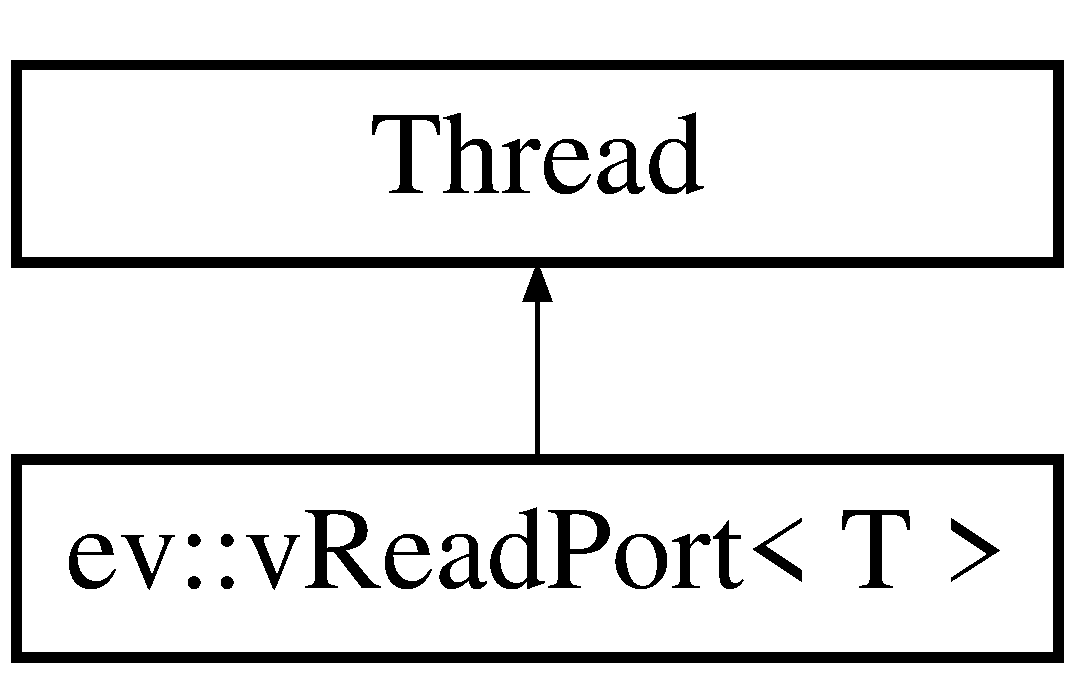
\includegraphics[height=2.000000cm]{classev_1_1vReadPort}
\end{center}
\end{figure}
\subsection*{Public Member Functions}
\begin{DoxyCompactItemize}
\item 
\mbox{\Hypertarget{classev_1_1vReadPort_a8c559db85d642d2779d2ea02acf75bc9}\label{classev_1_1vReadPort_a8c559db85d642d2779d2ea02acf75bc9}} 
\hyperlink{classev_1_1vReadPort_a8c559db85d642d2779d2ea02acf75bc9}{v\+Read\+Port} ()
\begin{DoxyCompactList}\small\item\em constructor \end{DoxyCompactList}\item 
\mbox{\Hypertarget{classev_1_1vReadPort_a7ce21badb00708a6914d8620bf17c797}\label{classev_1_1vReadPort_a7ce21badb00708a6914d8620bf17c797}} 
\hyperlink{classev_1_1vReadPort_a7ce21badb00708a6914d8620bf17c797}{$\sim$v\+Read\+Port} ()
\begin{DoxyCompactList}\small\item\em desctructor \end{DoxyCompactList}\item 
\mbox{\Hypertarget{classev_1_1vReadPort_a73b4f47c06fac76af81d14a704b35fe4}\label{classev_1_1vReadPort_a73b4f47c06fac76af81d14a704b35fe4}} 
bool {\bfseries open} (std\+::string name)
\item 
\mbox{\Hypertarget{classev_1_1vReadPort_a3458fb297eee91f29aa6d719876181b7}\label{classev_1_1vReadPort_a3458fb297eee91f29aa6d719876181b7}} 
void {\bfseries interrupt} ()
\item 
\mbox{\Hypertarget{classev_1_1vReadPort_ab7356731a6a6818d52f77de0aff5e423}\label{classev_1_1vReadPort_ab7356731a6a6818d52f77de0aff5e423}} 
void {\bfseries resume} ()
\item 
\mbox{\Hypertarget{classev_1_1vReadPort_adcdefc13d430033e876351bd383866bc}\label{classev_1_1vReadPort_adcdefc13d430033e876351bd383866bc}} 
void {\bfseries close} ()
\item 
\mbox{\Hypertarget{classev_1_1vReadPort_a1ff6550f46135f4d0a4e08436d90fa26}\label{classev_1_1vReadPort_a1ff6550f46135f4d0a4e08436d90fa26}} 
void {\bfseries on\+Stop} ()
\item 
\mbox{\Hypertarget{classev_1_1vReadPort_a383d2b1d3f896fce2fa352f76fe2fefb}\label{classev_1_1vReadPort_a383d2b1d3f896fce2fa352f76fe2fefb}} 
void {\bfseries run} ()
\item 
\mbox{\Hypertarget{classev_1_1vReadPort_a2c6aabe520b140ff5c6bc5f8231cadd5}\label{classev_1_1vReadPort_a2c6aabe520b140ff5c6bc5f8231cadd5}} 
const T $\ast$ \hyperlink{classev_1_1vReadPort_a2c6aabe520b140ff5c6bc5f8231cadd5}{read} (yarp\+::os\+::\+Stamp \&yarpstamp, bool wait=true)
\begin{DoxyCompactList}\small\item\em ask for a pointer to the next v\+Queue. if wait is true Blocks if no data is ready. \end{DoxyCompactList}\item 
\mbox{\Hypertarget{classev_1_1vReadPort_a1f8d56c7a4ec77f622c448c46c65afd8}\label{classev_1_1vReadPort_a1f8d56c7a4ec77f622c448c46c65afd8}} 
void \hyperlink{classev_1_1vReadPort_a1f8d56c7a4ec77f622c448c46c65afd8}{set\+Q\+Limit} (unsigned int number\+\_\+of\+\_\+qs)
\begin{DoxyCompactList}\small\item\em set the maximum number of qs that can be stored in the buffer. A value of 0 keeps all qs. \end{DoxyCompactList}\item 
\mbox{\Hypertarget{classev_1_1vReadPort_ab451342e9bc479c3db4a937ce41f7795}\label{classev_1_1vReadPort_ab451342e9bc479c3db4a937ce41f7795}} 
void \hyperlink{classev_1_1vReadPort_ab451342e9bc479c3db4a937ce41f7795}{release\+Data\+Lock} ()
\begin{DoxyCompactList}\small\item\em un\+Blocks the blocking call in get\+NextQ. Useful to ensure a graceful shutdown. No guarantee the return of get\+NextQ will be valid. \end{DoxyCompactList}\item 
\mbox{\Hypertarget{classev_1_1vReadPort_a43a2b8ca3db8938e8200072de2957ef8}\label{classev_1_1vReadPort_a43a2b8ca3db8938e8200072de2957ef8}} 
unsigned int \hyperlink{classev_1_1vReadPort_a43a2b8ca3db8938e8200072de2957ef8}{queryunprocessed} ()
\begin{DoxyCompactList}\small\item\em ask for the number of v\+Queues currently allocated. \end{DoxyCompactList}\item 
\mbox{\Hypertarget{classev_1_1vReadPort_a61466cf1cfcd794c5735c8bcc43dd8b5}\label{classev_1_1vReadPort_a61466cf1cfcd794c5735c8bcc43dd8b5}} 
unsigned int \hyperlink{classev_1_1vReadPort_a61466cf1cfcd794c5735c8bcc43dd8b5}{query\+DelayN} ()
\begin{DoxyCompactList}\small\item\em ask for the number of events in all v\+Queues. \end{DoxyCompactList}\item 
\mbox{\Hypertarget{classev_1_1vReadPort_ab84604a7b938a15a67c7db82d1bc82ac}\label{classev_1_1vReadPort_ab84604a7b938a15a67c7db82d1bc82ac}} 
double \hyperlink{classev_1_1vReadPort_ab84604a7b938a15a67c7db82d1bc82ac}{query\+DelayT} ()
\begin{DoxyCompactList}\small\item\em ask for the total time spanned by all v\+Queues. \end{DoxyCompactList}\item 
\mbox{\Hypertarget{classev_1_1vReadPort_af78cee18124aa9f6729aed6b8de529a5}\label{classev_1_1vReadPort_af78cee18124aa9f6729aed6b8de529a5}} 
double \hyperlink{classev_1_1vReadPort_af78cee18124aa9f6729aed6b8de529a5}{query\+Rate} ()
\begin{DoxyCompactList}\small\item\em ask for the high precision event rate \end{DoxyCompactList}\item 
\mbox{\Hypertarget{classev_1_1vReadPort_abfafe13fd97b9a2f86b0c16f9f77f640}\label{classev_1_1vReadPort_abfafe13fd97b9a2f86b0c16f9f77f640}} 
std\+::string {\bfseries delay\+Stat\+String} ()
\item 
\mbox{\Hypertarget{classev_1_1vReadPort_a174e9ccf70d44d4230822b7558873630}\label{classev_1_1vReadPort_a174e9ccf70d44d4230822b7558873630}} 
void {\bfseries set\+Reporter} (Port\+Report \&reporter)
\end{DoxyCompactItemize}
\subsection*{Protected Attributes}
\begin{DoxyCompactItemize}
\item 
\mbox{\Hypertarget{classev_1_1vReadPort_a7d2052a556597fb452648acfc9c69c7c}\label{classev_1_1vReadPort_a7d2052a556597fb452648acfc9c69c7c}} 
\hyperlink{classev_1_1vPortableInterface}{v\+Portable\+Interface} {\bfseries internal\+\_\+storage}
\item 
\mbox{\Hypertarget{classev_1_1vReadPort_af7dc70719d3d3b747410cac249375cd1}\label{classev_1_1vReadPort_af7dc70719d3d3b747410cac249375cd1}} 
Port {\bfseries port}
\item 
\mbox{\Hypertarget{classev_1_1vReadPort_a16253ae31557093d1678bcf7b9907208}\label{classev_1_1vReadPort_a16253ae31557093d1678bcf7b9907208}} 
T $\ast$ {\bfseries working\+\_\+queue}
\item 
\mbox{\Hypertarget{classev_1_1vReadPort_a0a644757f74909b9ffc65cdf573c62a9}\label{classev_1_1vReadPort_a0a644757f74909b9ffc65cdf573c62a9}} 
deque$<$ T $\ast$$>$ {\bfseries qq}
\item 
\mbox{\Hypertarget{classev_1_1vReadPort_a1f90047aed50cbf8b76e0b75e2330eb1}\label{classev_1_1vReadPort_a1f90047aed50cbf8b76e0b75e2330eb1}} 
deque$<$ Stamp $>$ {\bfseries sq}
\item 
\mbox{\Hypertarget{classev_1_1vReadPort_a550f6ee0b8c13aa3f9a4e0e030896cff}\label{classev_1_1vReadPort_a550f6ee0b8c13aa3f9a4e0e030896cff}} 
deque$<$ int $>$ {\bfseries t\+\_\+q}
\item 
\mbox{\Hypertarget{classev_1_1vReadPort_ad71bb0a275e553468d7bedf1949dd2d1}\label{classev_1_1vReadPort_ad71bb0a275e553468d7bedf1949dd2d1}} 
deque$<$ int $>$ {\bfseries n\+\_\+q}
\item 
\mbox{\Hypertarget{classev_1_1vReadPort_a35bb3489d3fa7fe86c0ef7b563305976}\label{classev_1_1vReadPort_a35bb3489d3fa7fe86c0ef7b563305976}} 
Mutex {\bfseries m}
\item 
\mbox{\Hypertarget{classev_1_1vReadPort_a1481febbd2f80b1874090aea1365e9dd}\label{classev_1_1vReadPort_a1481febbd2f80b1874090aea1365e9dd}} 
Mutex {\bfseries read\+\_\+mutex}
\item 
\mbox{\Hypertarget{classev_1_1vReadPort_afbcd0f47ccdafcedc57a2f23d104a145}\label{classev_1_1vReadPort_afbcd0f47ccdafcedc57a2f23d104a145}} 
Semaphore {\bfseries dataavailable}
\item 
\mbox{\Hypertarget{classev_1_1vReadPort_a35f6fe719860861eaaf9b2ebc30ac99e}\label{classev_1_1vReadPort_a35f6fe719860861eaaf9b2ebc30ac99e}} 
unsigned int {\bfseries qlimit}
\item 
\mbox{\Hypertarget{classev_1_1vReadPort_acdcf63464771194e87d0fdd8226361a0}\label{classev_1_1vReadPort_acdcf63464771194e87d0fdd8226361a0}} 
unsigned int {\bfseries unprocdqs}
\item 
\mbox{\Hypertarget{classev_1_1vReadPort_af6ce0d204c3fc755b32a31cdcc3b55b0}\label{classev_1_1vReadPort_af6ce0d204c3fc755b32a31cdcc3b55b0}} 
unsigned int {\bfseries delay\+\_\+nv}
\item 
\mbox{\Hypertarget{classev_1_1vReadPort_a440488d899ba95a07ec610616ffc9cd2}\label{classev_1_1vReadPort_a440488d899ba95a07ec610616ffc9cd2}} 
long unsigned int {\bfseries delay\+\_\+t}
\item 
\mbox{\Hypertarget{classev_1_1vReadPort_a9888128c255eaf3cc2d528590b8bf12f}\label{classev_1_1vReadPort_a9888128c255eaf3cc2d528590b8bf12f}} 
double {\bfseries event\+\_\+rate}
\item 
\mbox{\Hypertarget{classev_1_1vReadPort_a6c737cc37c6a88eeaf01c62d82c40d3a}\label{classev_1_1vReadPort_a6c737cc37c6a88eeaf01c62d82c40d3a}} 
int {\bfseries p\+\_\+time}
\end{DoxyCompactItemize}


The documentation for this class was generated from the following file\+:\begin{DoxyCompactItemize}
\item 
/mnt/d/projects/event-\/driven/lib/include/event-\/driven/v\+Port.\+h\end{DoxyCompactItemize}

\hypertarget{classev_1_1vSurface}{}\section{ev\+:\+:v\+Surface Class Reference}
\label{classev_1_1vSurface}\index{ev\+::v\+Surface@{ev\+::v\+Surface}}


The v\+Window class holds a list of events for a period of time as specified. Event expiry is checked each time new events are added and expired events are removed. At any point in time a copy of the current list of events can be requested.  




{\ttfamily \#include $<$v\+Window\+\_\+basic.\+h$>$}

Inheritance diagram for ev\+:\+:v\+Surface\+:\begin{figure}[H]
\begin{center}
\leavevmode
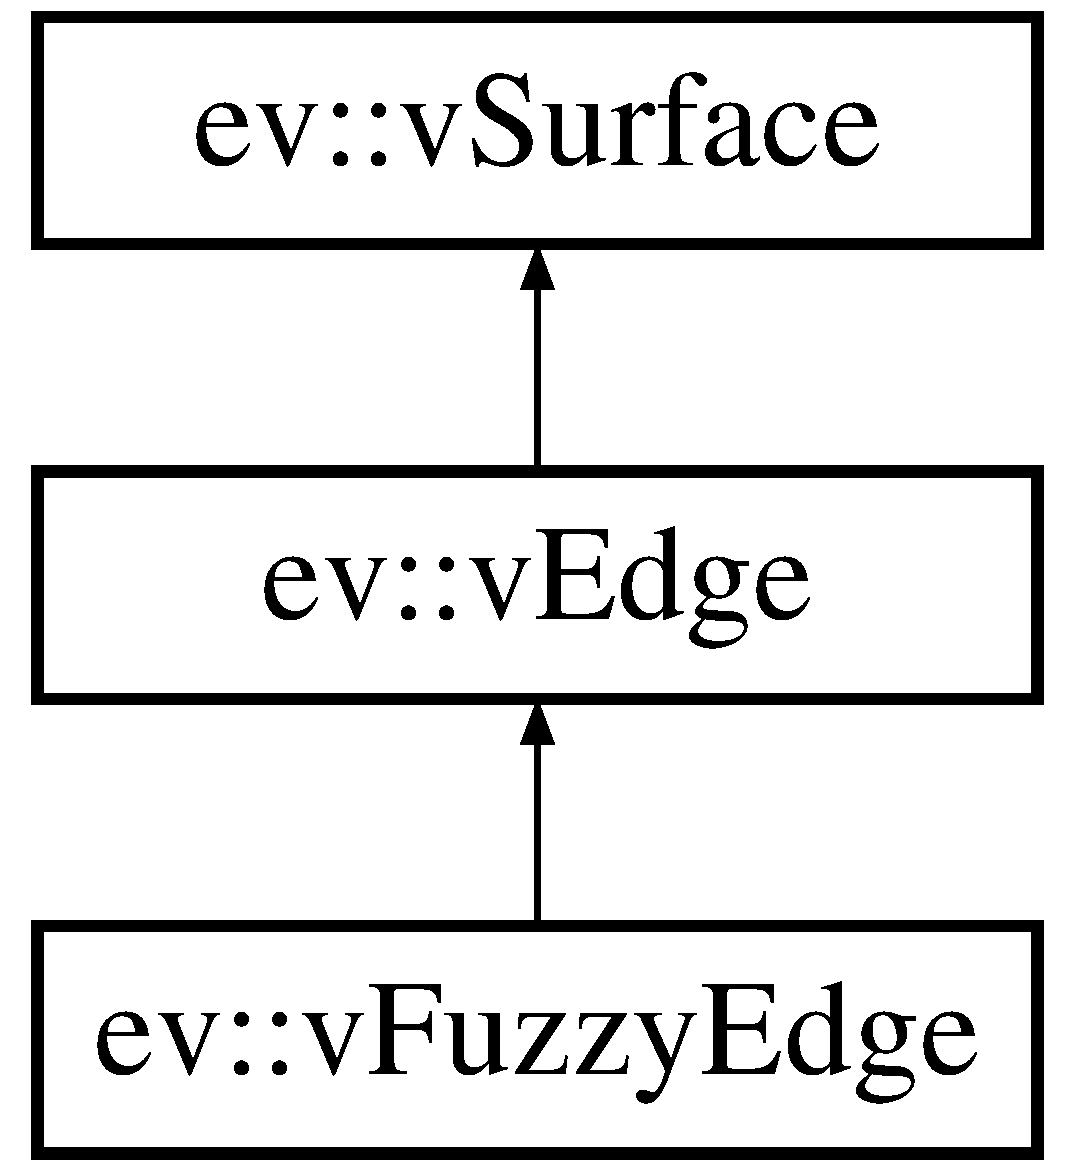
\includegraphics[height=3.000000cm]{classev_1_1vSurface}
\end{center}
\end{figure}
\subsection*{Public Member Functions}
\begin{DoxyCompactItemize}
\item 
\hyperlink{classev_1_1vSurface_afb642ce656aee165c54a2238474599c0}{v\+Surface} (int width=128, int height=128)
\begin{DoxyCompactList}\small\item\em v\+Window constructor \end{DoxyCompactList}\item 
\mbox{\Hypertarget{classev_1_1vSurface_a592c1c79ff294f34e28503d7c7278b8f}\label{classev_1_1vSurface_a592c1c79ff294f34e28503d7c7278b8f}} 
{\bfseries v\+Surface} (const \hyperlink{classev_1_1vSurface}{v\+Surface} \&)
\item 
\mbox{\Hypertarget{classev_1_1vSurface_af779bb51b4c9f748a0cd38117cf5e1f9}\label{classev_1_1vSurface_af779bb51b4c9f748a0cd38117cf5e1f9}} 
\hyperlink{classev_1_1vSurface}{v\+Surface} {\bfseries operator=} (const \hyperlink{classev_1_1vSurface}{v\+Surface} \&)
\item 
event$<$ \hyperlink{classev_1_1AddressEvent}{AE} $>$ \hyperlink{classev_1_1vSurface_a60d2f3d18c68d18678040cfabf6d35ea}{add\+Event} (event$<$ \hyperlink{classev_1_1AddressEvent}{AE} $>$ v)
\begin{DoxyCompactList}\small\item\em add\+Event adds an event to the window. Also checks for expired events. \end{DoxyCompactList}\item 
event$<$ \hyperlink{classev_1_1AddressEvent}{AE} $>$ \hyperlink{classev_1_1vSurface_a523c84d62fa48db30913dee7e694b895}{get\+Most\+Recent} ()
\begin{DoxyCompactList}\small\item\em get\+Most\+Recent \end{DoxyCompactList}\item 
\mbox{\Hypertarget{classev_1_1vSurface_aa90e7d977149ee42dff7a2735b367a2b}\label{classev_1_1vSurface_aa90e7d977149ee42dff7a2735b367a2b}} 
int {\bfseries get\+Event\+Count} ()
\item 
\mbox{\Hypertarget{classev_1_1vSurface_a222eadfa9d900d22148d1ffb0bb68661}\label{classev_1_1vSurface_a222eadfa9d900d22148d1ffb0bb68661}} 
void {\bfseries clear} ()
\item 
\mbox{\Hypertarget{classev_1_1vSurface_a2beddf5b5ffdbe12c1592ef8c1c742ab}\label{classev_1_1vSurface_a2beddf5b5ffdbe12c1592ef8c1c742ab}} 
const v\+Queue {\bfseries get\+Surf} (int d)
\item 
\mbox{\Hypertarget{classev_1_1vSurface_af6565b2434916ebc73820fb870e6f9a9}\label{classev_1_1vSurface_af6565b2434916ebc73820fb870e6f9a9}} 
const v\+Queue {\bfseries get\+Surf} (int x, int y, int d)
\item 
\mbox{\Hypertarget{classev_1_1vSurface_ae27682a1a876ef2c3b8c37c63c5a531c}\label{classev_1_1vSurface_ae27682a1a876ef2c3b8c37c63c5a531c}} 
virtual const v\+Queue {\bfseries get\+Surf} (int xl, int xh, int yl, int yh)
\end{DoxyCompactItemize}
\subsection*{Protected Attributes}
\begin{DoxyCompactItemize}
\item 
\mbox{\Hypertarget{classev_1_1vSurface_a157b4d26be73a1de42b0a043f12cf984}\label{classev_1_1vSurface_a157b4d26be73a1de42b0a043f12cf984}} 
std\+::vector$<$ std\+::vector$<$ event$<$ \hyperlink{classev_1_1AddressEvent}{AE} $>$ $>$ $>$ \hyperlink{classev_1_1vSurface_a157b4d26be73a1de42b0a043f12cf984}{spatial}
\begin{DoxyCompactList}\small\item\em for quick spatial accessing and surfacing \end{DoxyCompactList}\item 
\mbox{\Hypertarget{classev_1_1vSurface_a7ba9be674dbe03302b56306b987cff62}\label{classev_1_1vSurface_a7ba9be674dbe03302b56306b987cff62}} 
\hyperlink{structev_1_1resolution}{resolution} {\bfseries res}
\item 
\mbox{\Hypertarget{classev_1_1vSurface_a64339e84abccbb0099e0236fa4339647}\label{classev_1_1vSurface_a64339e84abccbb0099e0236fa4339647}} 
event$<$ \hyperlink{classev_1_1AddressEvent}{AE} $>$ {\bfseries most\+Recent}
\item 
\mbox{\Hypertarget{classev_1_1vSurface_a2b6a8d84a626b8dce15597807da598fb}\label{classev_1_1vSurface_a2b6a8d84a626b8dce15597807da598fb}} 
int {\bfseries event\+Count}
\end{DoxyCompactItemize}


\subsection{Detailed Description}
The v\+Window class holds a list of events for a period of time as specified. Event expiry is checked each time new events are added and expired events are removed. At any point in time a copy of the current list of events can be requested. 

\subsection{Constructor \& Destructor Documentation}
\mbox{\Hypertarget{classev_1_1vSurface_afb642ce656aee165c54a2238474599c0}\label{classev_1_1vSurface_afb642ce656aee165c54a2238474599c0}} 
\index{ev\+::v\+Surface@{ev\+::v\+Surface}!v\+Surface@{v\+Surface}}
\index{v\+Surface@{v\+Surface}!ev\+::v\+Surface@{ev\+::v\+Surface}}
\subsubsection{\texorpdfstring{v\+Surface()}{vSurface()}}
{\footnotesize\ttfamily ev\+::v\+Surface\+::v\+Surface (\begin{DoxyParamCaption}\item[{int}]{width = {\ttfamily 128},  }\item[{int}]{height = {\ttfamily 128} }\end{DoxyParamCaption})}



v\+Window constructor 


\begin{DoxyParams}{Parameters}
{\em window\+Size} & optional time to store events (in us) \\
\hline
\end{DoxyParams}


\subsection{Member Function Documentation}
\mbox{\Hypertarget{classev_1_1vSurface_a60d2f3d18c68d18678040cfabf6d35ea}\label{classev_1_1vSurface_a60d2f3d18c68d18678040cfabf6d35ea}} 
\index{ev\+::v\+Surface@{ev\+::v\+Surface}!add\+Event@{add\+Event}}
\index{add\+Event@{add\+Event}!ev\+::v\+Surface@{ev\+::v\+Surface}}
\subsubsection{\texorpdfstring{add\+Event()}{addEvent()}}
{\footnotesize\ttfamily event$<$ \hyperlink{classev_1_1AddressEvent}{AE} $>$ ev\+::v\+Surface\+::add\+Event (\begin{DoxyParamCaption}\item[{event$<$ \hyperlink{classev_1_1AddressEvent}{AE} $>$}]{v }\end{DoxyParamCaption})}



add\+Event adds an event to the window. Also checks for expired events. 


\begin{DoxyParams}{Parameters}
{\em event} & the event to add \\
\hline
\end{DoxyParams}
\mbox{\Hypertarget{classev_1_1vSurface_a523c84d62fa48db30913dee7e694b895}\label{classev_1_1vSurface_a523c84d62fa48db30913dee7e694b895}} 
\index{ev\+::v\+Surface@{ev\+::v\+Surface}!get\+Most\+Recent@{get\+Most\+Recent}}
\index{get\+Most\+Recent@{get\+Most\+Recent}!ev\+::v\+Surface@{ev\+::v\+Surface}}
\subsubsection{\texorpdfstring{get\+Most\+Recent()}{getMostRecent()}}
{\footnotesize\ttfamily event$<$ \hyperlink{classev_1_1AddressEvent}{AE} $>$ ev\+::v\+Surface\+::get\+Most\+Recent (\begin{DoxyParamCaption}{ }\end{DoxyParamCaption})}



get\+Most\+Recent 

\begin{DoxyReturn}{Returns}

\end{DoxyReturn}


The documentation for this class was generated from the following files\+:\begin{DoxyCompactItemize}
\item 
/mnt/d/projects/event-\/driven/lib/include/event-\/driven/v\+Window\+\_\+basic.\+h\item 
/mnt/d/projects/event-\/driven/lib/src/v\+Window\+\_\+basic.\+cpp\end{DoxyCompactItemize}

\hypertarget{classev_1_1vSurface2}{}\section{ev\+:\+:v\+Surface2 Class Reference}
\label{classev_1_1vSurface2}\index{ev\+::v\+Surface2@{ev\+::v\+Surface2}}


a spatial-\/temporal surface storage data structure  




{\ttfamily \#include $<$v\+Window\+\_\+adv.\+h$>$}

Inheritance diagram for ev\+:\+:v\+Surface2\+:\begin{figure}[H]
\begin{center}
\leavevmode
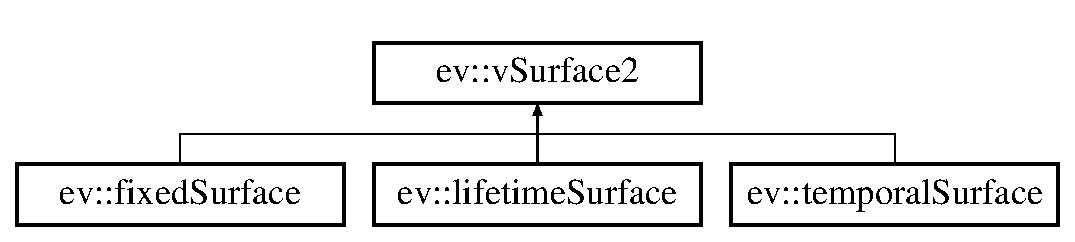
\includegraphics[height=2.000000cm]{classev_1_1vSurface2}
\end{center}
\end{figure}
\subsection*{Public Member Functions}
\begin{DoxyCompactItemize}
\item 
\hyperlink{classev_1_1vSurface2_ada6aeb852479aa111b1f5ad32ac1286b}{v\+Surface2} (int \hyperlink{classev_1_1vSurface2_a1aa8027816352a15d5b9bf1f26f48e76}{width}=128, int height=128)
\begin{DoxyCompactList}\small\item\em v\+Window constructor \end{DoxyCompactList}\item 
virtual v\+Queue \hyperlink{classev_1_1vSurface2_a6dee662976048b73d7b19e45871352da}{add\+Event} (event$<$$>$ v)
\begin{DoxyCompactList}\small\item\em add\+Event adds an event to the window. Also checks for expired events. \end{DoxyCompactList}\item 
\mbox{\Hypertarget{classev_1_1vSurface2_a311f0fb7297ee4a070755308e9271398}\label{classev_1_1vSurface2_a311f0fb7297ee4a070755308e9271398}} 
void {\bfseries fast\+Add\+Event} (event$<$$>$ v, bool only\+Add=false)
\item 
\mbox{\Hypertarget{classev_1_1vSurface2_af35870c14a5c94dc7522bdfcf76df2cb}\label{classev_1_1vSurface2_af35870c14a5c94dc7522bdfcf76df2cb}} 
virtual v\+Queue {\bfseries remove\+Events} (event$<$$>$ to\+Add)=0
\item 
\mbox{\Hypertarget{classev_1_1vSurface2_a956e6ab8f419554958961fbbca68029b}\label{classev_1_1vSurface2_a956e6ab8f419554958961fbbca68029b}} 
virtual void {\bfseries fast\+Remove\+Events} (event$<$$>$ to\+Add)=0
\item 
event \hyperlink{classev_1_1vSurface2_af84a860e057aea43831e8e6d16107cd4}{get\+Most\+Recent} ()
\begin{DoxyCompactList}\small\item\em get\+Most\+Recent \end{DoxyCompactList}\item 
\mbox{\Hypertarget{classev_1_1vSurface2_a67906f1ecd7fab30f1d0f7218388234e}\label{classev_1_1vSurface2_a67906f1ecd7fab30f1d0f7218388234e}} 
int {\bfseries get\+Event\+Count} ()
\item 
\mbox{\Hypertarget{classev_1_1vSurface2_a7897c4e7c034f36f86d29e14e36c2ca4}\label{classev_1_1vSurface2_a7897c4e7c034f36f86d29e14e36c2ca4}} 
v\+Queue {\bfseries get\+Everything} ()
\item 
v\+Queue \hyperlink{classev_1_1vSurface2_aedcc28d0ccdbc343f031506a8fa84bb0}{get\+Surf} ()
\begin{DoxyCompactList}\small\item\em get\+Window \end{DoxyCompactList}\item 
\mbox{\Hypertarget{classev_1_1vSurface2_aaa5978b3d040e278db563495585adf86}\label{classev_1_1vSurface2_aaa5978b3d040e278db563495585adf86}} 
v\+Queue {\bfseries get\+Surf} (int d)
\item 
v\+Queue \hyperlink{classev_1_1vSurface2_a42f7a69a075225254ffddc7bb5d4d9ba}{get\+Surf} (int x, int y, int d)
\begin{DoxyCompactList}\small\item\em get\+Spatial\+Window returns Address\+Events within a spatial window \end{DoxyCompactList}\item 
v\+Queue \hyperlink{classev_1_1vSurface2_aa74adc0c56d62a6f51c2901ec209233e}{get\+Surf} (int xl, int xh, int yl, int yh)
\begin{DoxyCompactList}\small\item\em get\+Spatial\+Window returns Address\+Events within a spatial window \end{DoxyCompactList}\item 
\mbox{\Hypertarget{classev_1_1vSurface2_a70e292820956b12c3bc123c4e724e90a}\label{classev_1_1vSurface2_a70e292820956b12c3bc123c4e724e90a}} 
v\+Queue {\bfseries get\+Surf\+\_\+\+Tlim} (int dt)
\item 
\mbox{\Hypertarget{classev_1_1vSurface2_ad487a13d9bcd8433489fb7e7b3fa5dc8}\label{classev_1_1vSurface2_ad487a13d9bcd8433489fb7e7b3fa5dc8}} 
v\+Queue {\bfseries get\+Surf\+\_\+\+Tlim} (int dt, int d)
\item 
\mbox{\Hypertarget{classev_1_1vSurface2_a53939fc4b201eaee766114982d0ae9c2}\label{classev_1_1vSurface2_a53939fc4b201eaee766114982d0ae9c2}} 
v\+Queue {\bfseries get\+Surf\+\_\+\+Tlim} (int dt, int x, int y, int d)
\item 
\mbox{\Hypertarget{classev_1_1vSurface2_a63c601ec2570dbde037c9ea92342b24b}\label{classev_1_1vSurface2_a63c601ec2570dbde037c9ea92342b24b}} 
v\+Queue {\bfseries get\+Surf\+\_\+\+Tlim} (int dt, int xl, int xh, int yl, int yh)
\item 
\mbox{\Hypertarget{classev_1_1vSurface2_acb41c1eff67ff285be715f8504d37d22}\label{classev_1_1vSurface2_acb41c1eff67ff285be715f8504d37d22}} 
v\+Queue {\bfseries get\+Surf\+\_\+\+Clim} (int c)
\item 
\mbox{\Hypertarget{classev_1_1vSurface2_af9e9a30828d508f49921b02224723a36}\label{classev_1_1vSurface2_af9e9a30828d508f49921b02224723a36}} 
v\+Queue {\bfseries get\+Surf\+\_\+\+Clim} (int c, int d)
\item 
\mbox{\Hypertarget{classev_1_1vSurface2_a708416f0ae3b13858f1c96e203898223}\label{classev_1_1vSurface2_a708416f0ae3b13858f1c96e203898223}} 
v\+Queue {\bfseries get\+Surf\+\_\+\+Clim} (int c, int x, int y, int d)
\item 
\mbox{\Hypertarget{classev_1_1vSurface2_a1b04ff8d8d449b054a514c092bac1145}\label{classev_1_1vSurface2_a1b04ff8d8d449b054a514c092bac1145}} 
v\+Queue {\bfseries get\+Surf\+\_\+\+Clim} (int c, int xl, int xh, int yl, int yh)
\item 
\mbox{\Hypertarget{classev_1_1vSurface2_aacd14a2e5c73e557b7b6b90a20624e23}\label{classev_1_1vSurface2_aacd14a2e5c73e557b7b6b90a20624e23}} 
void {\bfseries get\+Surf\+Sorted} (v\+Queue \&fillq)
\end{DoxyCompactItemize}
\subsection*{Protected Attributes}
\begin{DoxyCompactItemize}
\item 
\mbox{\Hypertarget{classev_1_1vSurface2_ad26e2a77d859924e39526fe69ad6e8bf}\label{classev_1_1vSurface2_ad26e2a77d859924e39526fe69ad6e8bf}} 
v\+Queue \hyperlink{classev_1_1vSurface2_ad26e2a77d859924e39526fe69ad6e8bf}{q}
\begin{DoxyCompactList}\small\item\em event storage \end{DoxyCompactList}\item 
\mbox{\Hypertarget{classev_1_1vSurface2_aeea3647a3da9c08bd0f3bd577e6ba443}\label{classev_1_1vSurface2_aeea3647a3da9c08bd0f3bd577e6ba443}} 
std\+::vector$<$ std\+::vector$<$ event$<$$>$ $>$ $>$ \hyperlink{classev_1_1vSurface2_aeea3647a3da9c08bd0f3bd577e6ba443}{spatial}
\begin{DoxyCompactList}\small\item\em for quick spatial accessing and surfacing \end{DoxyCompactList}\item 
\mbox{\Hypertarget{classev_1_1vSurface2_a1aa8027816352a15d5b9bf1f26f48e76}\label{classev_1_1vSurface2_a1aa8027816352a15d5b9bf1f26f48e76}} 
int \hyperlink{classev_1_1vSurface2_a1aa8027816352a15d5b9bf1f26f48e76}{width}
\begin{DoxyCompactList}\small\item\em retina size \end{DoxyCompactList}\item 
\mbox{\Hypertarget{classev_1_1vSurface2_a4cac3483eefdbe9e83ced2ef6bc5f7b2}\label{classev_1_1vSurface2_a4cac3483eefdbe9e83ced2ef6bc5f7b2}} 
int {\bfseries height}
\item 
\mbox{\Hypertarget{classev_1_1vSurface2_a53cfa9932bf60007440cbf535c115222}\label{classev_1_1vSurface2_a53cfa9932bf60007440cbf535c115222}} 
int \hyperlink{classev_1_1vSurface2_a53cfa9932bf60007440cbf535c115222}{count}
\begin{DoxyCompactList}\small\item\em active events \end{DoxyCompactList}\end{DoxyCompactItemize}


\subsection{Detailed Description}
a spatial-\/temporal surface storage data structure 

\subsection{Constructor \& Destructor Documentation}
\mbox{\Hypertarget{classev_1_1vSurface2_ada6aeb852479aa111b1f5ad32ac1286b}\label{classev_1_1vSurface2_ada6aeb852479aa111b1f5ad32ac1286b}} 
\index{ev\+::v\+Surface2@{ev\+::v\+Surface2}!v\+Surface2@{v\+Surface2}}
\index{v\+Surface2@{v\+Surface2}!ev\+::v\+Surface2@{ev\+::v\+Surface2}}
\subsubsection{\texorpdfstring{v\+Surface2()}{vSurface2()}}
{\footnotesize\ttfamily ev\+::v\+Surface2\+::v\+Surface2 (\begin{DoxyParamCaption}\item[{int}]{width = {\ttfamily 128},  }\item[{int}]{height = {\ttfamily 128} }\end{DoxyParamCaption})}



v\+Window constructor 


\begin{DoxyParams}{Parameters}
{\em window\+Size} & optional time to store events (in us) \\
\hline
\end{DoxyParams}


\subsection{Member Function Documentation}
\mbox{\Hypertarget{classev_1_1vSurface2_a6dee662976048b73d7b19e45871352da}\label{classev_1_1vSurface2_a6dee662976048b73d7b19e45871352da}} 
\index{ev\+::v\+Surface2@{ev\+::v\+Surface2}!add\+Event@{add\+Event}}
\index{add\+Event@{add\+Event}!ev\+::v\+Surface2@{ev\+::v\+Surface2}}
\subsubsection{\texorpdfstring{add\+Event()}{addEvent()}}
{\footnotesize\ttfamily v\+Queue ev\+::v\+Surface2\+::add\+Event (\begin{DoxyParamCaption}\item[{event$<$$>$}]{v }\end{DoxyParamCaption})\hspace{0.3cm}{\ttfamily [virtual]}}



add\+Event adds an event to the window. Also checks for expired events. 


\begin{DoxyParams}{Parameters}
{\em event} & the event to add \\
\hline
\end{DoxyParams}


Reimplemented in \hyperlink{classev_1_1lifetimeSurface_a8fce037a13281c0e46c7d660e0ea2275}{ev\+::lifetime\+Surface}.

\mbox{\Hypertarget{classev_1_1vSurface2_af84a860e057aea43831e8e6d16107cd4}\label{classev_1_1vSurface2_af84a860e057aea43831e8e6d16107cd4}} 
\index{ev\+::v\+Surface2@{ev\+::v\+Surface2}!get\+Most\+Recent@{get\+Most\+Recent}}
\index{get\+Most\+Recent@{get\+Most\+Recent}!ev\+::v\+Surface2@{ev\+::v\+Surface2}}
\subsubsection{\texorpdfstring{get\+Most\+Recent()}{getMostRecent()}}
{\footnotesize\ttfamily event ev\+::v\+Surface2\+::get\+Most\+Recent (\begin{DoxyParamCaption}{ }\end{DoxyParamCaption})}



get\+Most\+Recent 

\begin{DoxyReturn}{Returns}

\end{DoxyReturn}
\mbox{\Hypertarget{classev_1_1vSurface2_aedcc28d0ccdbc343f031506a8fa84bb0}\label{classev_1_1vSurface2_aedcc28d0ccdbc343f031506a8fa84bb0}} 
\index{ev\+::v\+Surface2@{ev\+::v\+Surface2}!get\+Surf@{get\+Surf}}
\index{get\+Surf@{get\+Surf}!ev\+::v\+Surface2@{ev\+::v\+Surface2}}
\subsubsection{\texorpdfstring{get\+Surf()}{getSurf()}\hspace{0.1cm}{\footnotesize\ttfamily [1/3]}}
{\footnotesize\ttfamily v\+Queue ev\+::v\+Surface2\+::get\+Surf (\begin{DoxyParamCaption}{ }\end{DoxyParamCaption})}



get\+Window 

\begin{DoxyReturn}{Returns}

\end{DoxyReturn}
\mbox{\Hypertarget{classev_1_1vSurface2_a42f7a69a075225254ffddc7bb5d4d9ba}\label{classev_1_1vSurface2_a42f7a69a075225254ffddc7bb5d4d9ba}} 
\index{ev\+::v\+Surface2@{ev\+::v\+Surface2}!get\+Surf@{get\+Surf}}
\index{get\+Surf@{get\+Surf}!ev\+::v\+Surface2@{ev\+::v\+Surface2}}
\subsubsection{\texorpdfstring{get\+Surf()}{getSurf()}\hspace{0.1cm}{\footnotesize\ttfamily [2/3]}}
{\footnotesize\ttfamily v\+Queue ev\+::v\+Surface2\+::get\+Surf (\begin{DoxyParamCaption}\item[{int}]{x,  }\item[{int}]{y,  }\item[{int}]{d }\end{DoxyParamCaption})}



get\+Spatial\+Window returns Address\+Events within a spatial window 


\begin{DoxyParams}{Parameters}
{\em x} & x centre \\
\hline
{\em y} & y centre \\
\hline
{\em d} & distance of the half-\/length of a square window \\
\hline
\end{DoxyParams}
\begin{DoxyReturn}{Returns}
a v\+Queue containing a copy of the events 
\end{DoxyReturn}
\mbox{\Hypertarget{classev_1_1vSurface2_aa74adc0c56d62a6f51c2901ec209233e}\label{classev_1_1vSurface2_aa74adc0c56d62a6f51c2901ec209233e}} 
\index{ev\+::v\+Surface2@{ev\+::v\+Surface2}!get\+Surf@{get\+Surf}}
\index{get\+Surf@{get\+Surf}!ev\+::v\+Surface2@{ev\+::v\+Surface2}}
\subsubsection{\texorpdfstring{get\+Surf()}{getSurf()}\hspace{0.1cm}{\footnotesize\ttfamily [3/3]}}
{\footnotesize\ttfamily v\+Queue ev\+::v\+Surface2\+::get\+Surf (\begin{DoxyParamCaption}\item[{int}]{xl,  }\item[{int}]{xh,  }\item[{int}]{yl,  }\item[{int}]{yh }\end{DoxyParamCaption})}



get\+Spatial\+Window returns Address\+Events within a spatial window 


\begin{DoxyParams}{Parameters}
{\em xl} & lower x value of window \\
\hline
{\em xh} & upper x value of window \\
\hline
{\em yl} & lower y value of window \\
\hline
{\em yh} & upper y value of window \\
\hline
\end{DoxyParams}
\begin{DoxyReturn}{Returns}
a v\+Queue containing a copy of the events 
\end{DoxyReturn}


The documentation for this class was generated from the following files\+:\begin{DoxyCompactItemize}
\item 
/mnt/d/projects/event-\/driven/lib/include/event-\/driven/v\+Window\+\_\+adv.\+h\item 
/mnt/d/projects/event-\/driven/lib/src/v\+Window\+\_\+adv.\+cpp\end{DoxyCompactItemize}

\hypertarget{classev_1_1vTempWindow}{}\section{ev\+:\+:v\+Temp\+Window Class Reference}
\label{classev_1_1vTempWindow}\index{ev\+::v\+Temp\+Window@{ev\+::v\+Temp\+Window}}


store events for a fixed amount of time in a v\+Queue  




{\ttfamily \#include $<$v\+Window\+\_\+basic.\+h$>$}

Inheritance diagram for ev\+:\+:v\+Temp\+Window\+:\begin{figure}[H]
\begin{center}
\leavevmode
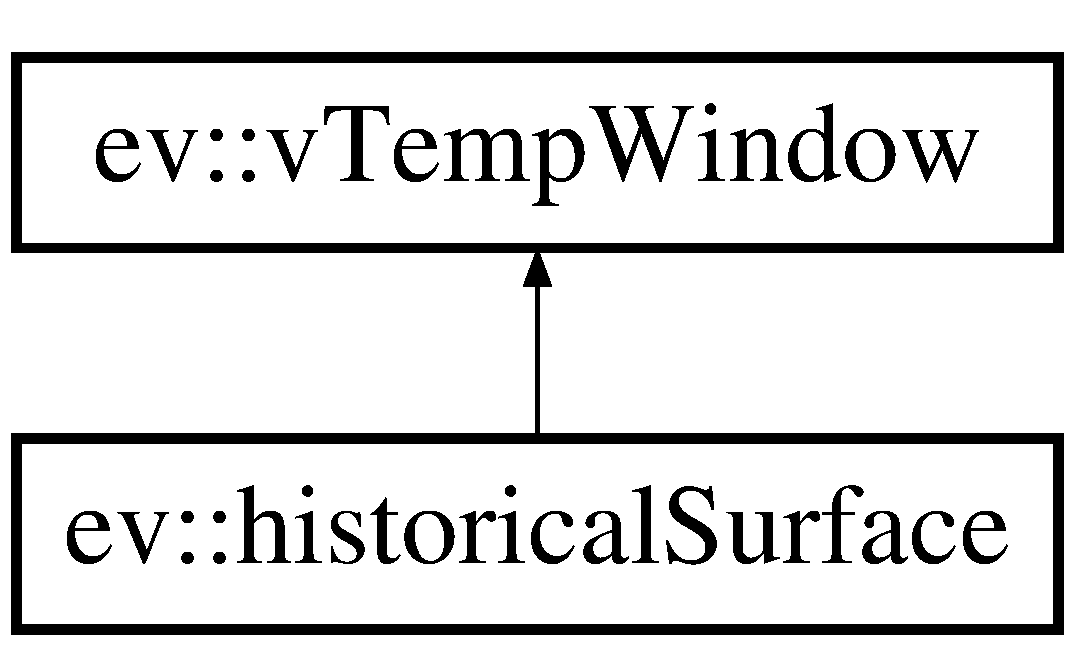
\includegraphics[height=2.000000cm]{classev_1_1vTempWindow}
\end{center}
\end{figure}
\subsection*{Public Member Functions}
\begin{DoxyCompactItemize}
\item 
\mbox{\Hypertarget{classev_1_1vTempWindow_a9499371e18cc811e2cd3e47e8e96f8ca}\label{classev_1_1vTempWindow_a9499371e18cc811e2cd3e47e8e96f8ca}} 
void {\bfseries add\+Event} (event$<$$>$ v)
\item 
\mbox{\Hypertarget{classev_1_1vTempWindow_a925ee62f3dff9517654fd6a9a402616b}\label{classev_1_1vTempWindow_a925ee62f3dff9517654fd6a9a402616b}} 
void {\bfseries add\+Events} (const v\+Queue \&events)
\item 
\mbox{\Hypertarget{classev_1_1vTempWindow_a40ddfc12e259c028a57d5dd188b3e2e9}\label{classev_1_1vTempWindow_a40ddfc12e259c028a57d5dd188b3e2e9}} 
v\+Queue {\bfseries get\+Window} ()
\end{DoxyCompactItemize}
\subsection*{Protected Attributes}
\begin{DoxyCompactItemize}
\item 
\mbox{\Hypertarget{classev_1_1vTempWindow_abed022ad51f68443a2350fbeabbb4233}\label{classev_1_1vTempWindow_abed022ad51f68443a2350fbeabbb4233}} 
v\+Queue \hyperlink{classev_1_1vTempWindow_abed022ad51f68443a2350fbeabbb4233}{q}
\begin{DoxyCompactList}\small\item\em event storage \end{DoxyCompactList}\item 
\mbox{\Hypertarget{classev_1_1vTempWindow_a909a8f6df0014d1f318c6209223f5fad}\label{classev_1_1vTempWindow_a909a8f6df0014d1f318c6209223f5fad}} 
int \hyperlink{classev_1_1vTempWindow_a909a8f6df0014d1f318c6209223f5fad}{t\+Upper}
\begin{DoxyCompactList}\small\item\em precalculated thresholds \end{DoxyCompactList}\item 
\mbox{\Hypertarget{classev_1_1vTempWindow_a47845a9e47b73598e2a325c06e994bed}\label{classev_1_1vTempWindow_a47845a9e47b73598e2a325c06e994bed}} 
int {\bfseries t\+Lower}
\end{DoxyCompactItemize}


\subsection{Detailed Description}
store events for a fixed amount of time in a v\+Queue 

The documentation for this class was generated from the following files\+:\begin{DoxyCompactItemize}
\item 
/mnt/d/projects/event-\/driven/lib/include/event-\/driven/v\+Window\+\_\+basic.\+h\item 
/mnt/d/projects/event-\/driven/lib/src/v\+Window\+\_\+basic.\+cpp\end{DoxyCompactItemize}

\hypertarget{classev_1_1vtsHelper}{}\section{ev\+:\+:vts\+Helper Class Reference}
\label{classev_1_1vtsHelper}\index{ev\+::vts\+Helper@{ev\+::vts\+Helper}}


helper class to deal with timestamp conversion and wrapping  




{\ttfamily \#include $<$vts\+Helper.\+h$>$}

\subsection*{Public Member Functions}
\begin{DoxyCompactItemize}
\item 
\mbox{\Hypertarget{classev_1_1vtsHelper_a44b5e8174eb7a317001e395bf0d917e8}\label{classev_1_1vtsHelper_a44b5e8174eb7a317001e395bf0d917e8}} 
\hyperlink{classev_1_1vtsHelper_a44b5e8174eb7a317001e395bf0d917e8}{vts\+Helper} ()
\begin{DoxyCompactList}\small\item\em constructor \end{DoxyCompactList}\item 
\mbox{\Hypertarget{classev_1_1vtsHelper_a399c3a719f7544209ba77f442c97c135}\label{classev_1_1vtsHelper_a399c3a719f7544209ba77f442c97c135}} 
unsigned long int \hyperlink{classev_1_1vtsHelper_a399c3a719f7544209ba77f442c97c135}{operator()} (int timestamp)
\begin{DoxyCompactList}\small\item\em unwrap a timestamp, given previously unwrapped timestamps \end{DoxyCompactList}\item 
\mbox{\Hypertarget{classev_1_1vtsHelper_ab8b7f4f4240f2a0f0279bda5f5f2caff}\label{classev_1_1vtsHelper_ab8b7f4f4240f2a0f0279bda5f5f2caff}} 
unsigned long int \hyperlink{classev_1_1vtsHelper_ab8b7f4f4240f2a0f0279bda5f5f2caff}{current\+Time} ()
\begin{DoxyCompactList}\small\item\em ask for the current unwrapped time, without updating the time. \end{DoxyCompactList}\end{DoxyCompactItemize}
\subsection*{Static Public Member Functions}
\begin{DoxyCompactItemize}
\item 
\mbox{\Hypertarget{classev_1_1vtsHelper_aa7f1c13eb051773e9413b52bb52caad0}\label{classev_1_1vtsHelper_aa7f1c13eb051773e9413b52bb52caad0}} 
static long int \hyperlink{classev_1_1vtsHelper_aa7f1c13eb051773e9413b52bb52caad0}{max\+Stamp} ()
\begin{DoxyCompactList}\small\item\em D\+E\+P\+R\+E\+C\+A\+T\+ED -\/ access to max\+\_\+stamp member variable is public. \end{DoxyCompactList}\item 
\mbox{\Hypertarget{classev_1_1vtsHelper_a07d0dc3cd7743eff7d594e838ae23a01}\label{classev_1_1vtsHelper_a07d0dc3cd7743eff7d594e838ae23a01}} 
static double \hyperlink{classev_1_1vtsHelper_a07d0dc3cd7743eff7d594e838ae23a01}{tstosecs} ()
\begin{DoxyCompactList}\small\item\em D\+E\+P\+R\+E\+C\+A\+T\+ED -\/ access to timestamp conversion member variables is public. \end{DoxyCompactList}\item 
\mbox{\Hypertarget{classev_1_1vtsHelper_a49e6d2f2f4c93f2ba8935630735c6fa5}\label{classev_1_1vtsHelper_a49e6d2f2f4c93f2ba8935630735c6fa5}} 
static int {\bfseries delta\+Ticks} (const int current\+\_\+tick, const int prev\+\_\+tick)
\item 
\mbox{\Hypertarget{classev_1_1vtsHelper_a398f00887ff3412590800a800ce6a052}\label{classev_1_1vtsHelper_a398f00887ff3412590800a800ce6a052}} 
static double {\bfseries delta\+MS} (const int current\+\_\+tick, const int prev\+\_\+tick)
\end{DoxyCompactItemize}
\subsection*{Static Public Attributes}
\begin{DoxyCompactItemize}
\item 
\mbox{\Hypertarget{classev_1_1vtsHelper_a059fdcf455b471e69446e565ed017f65}\label{classev_1_1vtsHelper_a059fdcf455b471e69446e565ed017f65}} 
static unsigned int \hyperlink{classev_1_1vtsHelper_a059fdcf455b471e69446e565ed017f65}{max\+\_\+stamp} = (1 $<$$<$ T\+I\+M\+E\+R\+\_\+\+B\+I\+TS) -\/ 1
\begin{DoxyCompactList}\small\item\em the maximum value of the timestamp before a wrap occurs \end{DoxyCompactList}\item 
\mbox{\Hypertarget{classev_1_1vtsHelper_ad3ad427d18c24f9655bbc73295abf678}\label{classev_1_1vtsHelper_ad3ad427d18c24f9655bbc73295abf678}} 
static double \hyperlink{classev_1_1vtsHelper_ad3ad427d18c24f9655bbc73295abf678}{tsscaler} = 0.\+000000001 $\ast$ C\+L\+O\+C\+K\+\_\+\+P\+E\+R\+I\+OD
\begin{DoxyCompactList}\small\item\em a multiplier to convert an event timestamp to seconds \end{DoxyCompactList}\item 
\mbox{\Hypertarget{classev_1_1vtsHelper_afa2dd46ae7113668bc6ebea88ab8fa11}\label{classev_1_1vtsHelper_afa2dd46ae7113668bc6ebea88ab8fa11}} 
static double \hyperlink{classev_1_1vtsHelper_afa2dd46ae7113668bc6ebea88ab8fa11}{vtsscaler} = 1.\+0 / \hyperlink{classev_1_1vtsHelper_ad3ad427d18c24f9655bbc73295abf678}{vts\+Helper\+::tsscaler}
\begin{DoxyCompactList}\small\item\em a multiplier to convert seconds to an event timestamp \end{DoxyCompactList}\end{DoxyCompactItemize}


\subsection{Detailed Description}
helper class to deal with timestamp conversion and wrapping 

The documentation for this class was generated from the following files\+:\begin{DoxyCompactItemize}
\item 
/mnt/d/projects/event-\/driven/lib/include/event-\/driven/vts\+Helper.\+h\item 
/mnt/d/projects/event-\/driven/lib/src/vts\+Helper.\+cpp\end{DoxyCompactItemize}

\hypertarget{classev_1_1vWritePort}{}\section{ev\+:\+:v\+Write\+Port Class Reference}
\label{classev_1_1vWritePort}\index{ev\+::v\+Write\+Port@{ev\+::v\+Write\+Port}}
\subsection*{Public Member Functions}
\begin{DoxyCompactItemize}
\item 
\mbox{\Hypertarget{classev_1_1vWritePort_a2ae9d0799444e6b08a2741632ca2a844}\label{classev_1_1vWritePort_a2ae9d0799444e6b08a2741632ca2a844}} 
bool {\bfseries open} (std\+::string name)
\item 
\mbox{\Hypertarget{classev_1_1vWritePort_a8657bd358f9714f5c183ba3038f1e672}\label{classev_1_1vWritePort_a8657bd358f9714f5c183ba3038f1e672}} 
void {\bfseries close} ()
\item 
\mbox{\Hypertarget{classev_1_1vWritePort_aaf5570455ab1a10e33005ea195f01212}\label{classev_1_1vWritePort_aaf5570455ab1a10e33005ea195f01212}} 
void {\bfseries set\+Write\+Type} (std\+::string tag)
\item 
\mbox{\Hypertarget{classev_1_1vWritePort_a82bdfad9b345a33f3458c82c65e62305}\label{classev_1_1vWritePort_a82bdfad9b345a33f3458c82c65e62305}} 
int {\bfseries get\+Output\+Count} ()
\item 
\mbox{\Hypertarget{classev_1_1vWritePort_a30e8556f5ab495ec11cb5f595d0fc679}\label{classev_1_1vWritePort_a30e8556f5ab495ec11cb5f595d0fc679}} 
bool {\bfseries write} (const vector$<$ int32\+\_\+t $>$ \&q, Stamp \&envelope)
\item 
\mbox{\Hypertarget{classev_1_1vWritePort_ae90dc683d47992ea2374237c130f057b}\label{classev_1_1vWritePort_ae90dc683d47992ea2374237c130f057b}} 
bool {\bfseries write} (const deque$<$ int32\+\_\+t $>$ \&q, Stamp \&envelope)
\item 
\mbox{\Hypertarget{classev_1_1vWritePort_aa3a656f3748b036cf2a632d9591c13f3}\label{classev_1_1vWritePort_aa3a656f3748b036cf2a632d9591c13f3}} 
bool {\bfseries write} (const v\+Queue \&q, Stamp \&envelope)
\item 
\mbox{\Hypertarget{classev_1_1vWritePort_a4accfe5230b426f9b863e481d8fb3c6c}\label{classev_1_1vWritePort_a4accfe5230b426f9b863e481d8fb3c6c}} 
{\footnotesize template$<$class T $>$ }\\bool {\bfseries write} (const std\+::deque$<$ T $>$ \&q, Stamp \&envelope)
\item 
\mbox{\Hypertarget{classev_1_1vWritePort_a1fbcfd268af4278ae3d778b5c1b0284a}\label{classev_1_1vWritePort_a1fbcfd268af4278ae3d778b5c1b0284a}} 
{\footnotesize template$<$class T $>$ }\\bool {\bfseries write} (const std\+::vector$<$ T $>$ \&q, Stamp \&envelope)
\end{DoxyCompactItemize}
\subsection*{Protected Member Functions}
\begin{DoxyCompactItemize}
\item 
\mbox{\Hypertarget{classev_1_1vWritePort_a05c3debed09851bd024782ca0e4a7b54}\label{classev_1_1vWritePort_a05c3debed09851bd024782ca0e4a7b54}} 
bool {\bfseries \+\_\+internal\+\_\+write} (Stamp \&envelope)
\end{DoxyCompactItemize}
\subsection*{Protected Attributes}
\begin{DoxyCompactItemize}
\item 
\mbox{\Hypertarget{classev_1_1vWritePort_af9ffcc74c80d4c04f2447c718c52f270}\label{classev_1_1vWritePort_af9ffcc74c80d4c04f2447c718c52f270}} 
\hyperlink{classev_1_1vPortableInterface}{v\+Portable\+Interface} {\bfseries internal\+\_\+storage}
\item 
\mbox{\Hypertarget{classev_1_1vWritePort_a0cb1d83ab6473e736660b9e95a5e35b9}\label{classev_1_1vWritePort_a0cb1d83ab6473e736660b9e95a5e35b9}} 
Port {\bfseries port}
\end{DoxyCompactItemize}


The documentation for this class was generated from the following file\+:\begin{DoxyCompactItemize}
\item 
/mnt/d/projects/event-\/driven/lib/include/event-\/driven/v\+Port.\+h\end{DoxyCompactItemize}

%--- End generated contents ---

% Index
\backmatter
\newpage
\phantomsection
\clearemptydoublepage
\addcontentsline{toc}{chapter}{Index}
\printindex

\end{document}
